\documentclass[11pt,a4paper]{article}

% 1. FONT & NGÔN NGỮ
\usepackage[T5]{fontenc}
\usepackage[utf8]{inputenc}
\usepackage{lmodern}
\usepackage[vietnamese]{babel}
\usepackage{indentfirst}

% 2. TOÁN HỌC & ĐỊNH LÝ

\usepackage{amsmath,amssymb,amsfonts}
\newtheorem{definition}{Định nghĩa}[section]
\newtheorem{theorem}{Định lý}[section]
\newtheorem{proof}{Chứng minh}[section]
\newtheorem{proposition}{Mệnh đề}[section]
\newtheorem{remark}[theorem]{Nhận xét}
\newtheorem{example}{Ví dụ}[section]
\newtheorem{corollary}[theorem]{Hệ quả}
\newtheorem{note}{Lưu ý}[section]
\usepackage{algorithm}
\usepackage{algpseudocode}
\usepackage{natbib}

% Việt hóa tên môi trường thuật toán
\floatname{algorithm}{Thuật toán}

% --- Khai báo Đầu vào / Đầu ra ---
\algrenewcommand\algorithmicrequire{\textbf{Đầu vào:}}
\algrenewcommand\algorithmicensure{\textbf{Kết quả:}}
\algrenewcommand\algorithmicreturn{\textbf{Trả về}}

% --- Cấu trúc rẽ nhánh (Điều kiện) ---
\algrenewcommand\algorithmicif{\textbf{nếu}}
\algrenewcommand\algorithmicthen{\textbf{thì}}
\algrenewcommand\algorithmicelse{\textbf{ngược lại}}

% --- Cấu trúc vòng lặp ---
\algrenewcommand\algorithmicfor{\textbf{với}}
\algrenewcommand\algorithmicwhile{\textbf{trong khi}}
\algrenewcommand\algorithmicdo{\textbf{thực hiện}}
\algrenewcommand\algorithmicrepeat{\textbf{lặp}}
\algrenewcommand\algorithmicuntil{\textbf{cho đến khi}}

% --- Kết thúc block ---
\algrenewcommand\algorithmicend{\textbf{kết thúc}}

% 3. ĐỒ HỌA & VẼ HÌNH (THÊM CHO TRANG BÌA)
\usepackage{graphicx}
\usepackage{tikz}
\usetikzlibrary{calc}
\usetikzlibrary{arrows.meta, positioning}

% 4. CĂN LỀ & BỐ CỤC TRANG
\usepackage[top=2.5cm, bottom=2.5cm, left=3cm, right=2.5cm]{geometry}
\usepackage{setspace}
\setstretch{1.25}
\usepackage{float}
\usepackage{booktabs} % Dùng cho \toprule, \midrule, \bottomrule
\usepackage{tabularx} % Dùng để tự động căn chỉnh độ rộng cột vừa với trang
\usepackage{array}    % Dùng để tùy chỉnh căn lề trong cộtV
\usepackage{enumitem}
\setlist[itemize]{leftmargin=*, itemsep=0.4em, topsep=0.3em}

% 5. MÀU SẮC & ĐỊNH DẠNG TIÊU ĐỀ
\usepackage{xcolor}
% Màu tiêu đề và liên kết
\definecolor{titleblue}{RGB}{35, 75, 135}
\definecolor{linkblue}{RGB}{0, 102, 204}
% Màu cho Code (Listings)
\definecolor{codegreen}{RGB}{0,120,0}
\definecolor{codegray}{RGB}{110,110,110}
\definecolor{codeblue}{RGB}{0,0,180}
\definecolor{backcolour}{RGB}{248,248,248}
% Màu cho Tcolorbox
\definecolor{XanhTieuDe}{RGB}{0, 102, 34} 
\definecolor{XanhNen}{RGB}{234, 245, 238}

\usepackage{titlesec}
\titleformat{\section}{\normalfont\Large\bfseries\color{titleblue}}{\thesection.}{0.5em}{}
\titleformat{\subsection}{\normalfont\large\bfseries\color{titleblue}}{\thesubsection.}{0.5em}{}
\titleformat{\subsubsection}{\normalfont\large\bfseries\color{titleblue}}{\thesubsubsection.}{0.5em}{}

% 6. CẤU HÌNH HIỂN THỊ CODE (LISTINGS)
\usepackage{listings}
\renewcommand{\lstlistingname}{Đoạn mã}
\usepackage{xcolor}

% Định nghĩa màu sắc (Bắt buộc để không bị lỗi Missing color name)
\definecolor{codegreen}{rgb}{0,0.6,0}
\definecolor{codegray}{rgb}{0.5,0.5,0.5}
\definecolor{backcolour}{rgb}{0.95,0.95,0.92}

% Định nghĩa style cho Matlab
\lstdefinestyle{MatlabStyle}{
    language=Matlab,
    backgroundcolor=\color{backcolour},
    basicstyle=\ttfamily\small,
    keywordstyle=\color{blue}\bfseries,
    commentstyle=\color{codegreen}\itshape,
    stringstyle=\color{red},
    numbers=left,
    numberstyle=\tiny\color{codegray},
    stepnumber=1,
    numbersep=10pt,
    frame=single,
    framesep=8pt,
    rulecolor=\color{gray},
    breaklines=true,
    breakatwhitespace=true,
    showstringspaces=false,
    tabsize=4,
    columns=fullflexible,
    keepspaces=true
}

% Kích hoạt style vừa tạo làm mặc định (tùy chọn)
\lstset{style=MatlabStyle}

% 7. MÔI TRƯỜNG ĐÓNG KHUNG
% \usepackage[most]{tcolorbox}
% \usepackage{pgfkeys}

% \newtcolorbox{baitapbox}[1]{
%     colback=blue!5, 
%     colframe=blue!60!black, 
%     coltitle=white, 
%     fonttitle=\bfseries, 
%     enhanced, 
%     title=#1
% }

% \newtcolorbox{vidu}[1]{
%     colback=XanhNen, 
%     colframe=XanhTieuDe, 
%     coltitle=white,
%     fonttitle=\bfseries, 
%     title=#1
% }

% \newtcolorbox{bode}[1]{ 
%     enhanced, 
%     colback=red!5!white, 
%     colframe=red, 
%     boxrule=0.5pt,
%     arc=2mm,
%     title={#1}, 
%     fonttitle=\bfseries, 
%     colbacktitle=red,
%     attach boxed title to top left={xshift=5mm, yshift=-2.5mm}, 
%     boxed title style={arc=3mm, size=small}
% }

\newcommand{\ngaythangnam}[3]{ngày #1 tháng #2 năm #3}

% 9. HYPERREF
\usepackage{hyperref}
\hypersetup{
    colorlinks=true,
    linkcolor=titleblue,
    filecolor=magenta,      
    urlcolor=linkblue,
}

\usepackage[backend=biber, style=ieee, language=english]{biblatex}
\addbibresource{references.bib} 

\begin{document}

% ----------------- TRANG BÌA -------
\begin{titlepage}
    \begin{center}
        {\Large ĐẠI HỌC QUỐC GIA THÀNH PHỐ HỒ CHÍ MINH}\\
        {\Large TRƯỜNG ĐẠI HỌC KHOA HỌC TỰ NHIÊN}\\
        {\Large KHOA TOÁN - TIN HỌC}\\[1.5cm]
        
        
\includegraphics[scale=0.27]{Images/04_Images/logo.jpg}\\[2cm]
        
        { \Large \bfseries MẠNG NƠ-RON TRUYỀN THẲNG\\[2cm] }
        
        {\large SEMINAR GIẢI TÍCH SỐ}\\[0.5cm]
        
        \begin{tabular}{l l}
            \textbf{GIẢNG VIÊN HƯỚNG DẪN:} & TS. Ông Thanh Hải \\
            \textbf{SINH VIÊN THỰC HIỆN:} & Nguyễn Hoàng Tú
        \end{tabular}
        
        \begin{tikzpicture}[remember picture, overlay]
            \draw[line width = 2pt] ($(current page.north west) + (2cm,-2cm)$) rectangle ($(current page.south east) + (-1.5cm,2cm)$);
        \end{tikzpicture}
        
        \vfill
        
        TP. Hồ Chí Minh, \ngaythangnam{08}{10}{2026}
        
    \end{center}
\end{titlepage}
% -----------------------------------
\tableofcontents
\newpage 
\section{Mạng nơ-ron truyền thẳng đa tầng}
\subsection{Nơ-ron nhân tạo}

\begin{figure}[H]
    \centering
    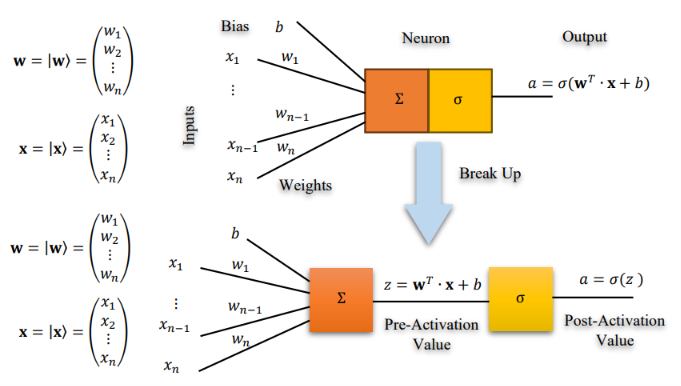
\includegraphics[width=0.8\linewidth]{Images/04_Images/1.png}
    \caption{Các giá trị trước và sau kích hoạt bên trong một nơ-ron.}
    \label{4.1}
\end{figure}
 
Về mặt toán học, một nơ-ron nhân tạo được biểu diễn như một hàm số $f: \mathbb{R}^d \to \mathbb{R}$, ánh xạ từ véc-tơ đầu vào $\mathbf{x} \in \mathbb{R}^d$ sang một giá trị đầu ra vô hướng $a \in \mathbb{R}$. 
Nơ-ron này được tham số hóa bởi một véc-tơ trọng số $\mathbf{w} = [w_1, w_2, \dots, w_d]^\top \in \mathbb{R}^d$ và một độ chệch vô hướng $b \in \mathbb{R}$. Quá trình xử lý và tạo thông tin đầu ra tại một nơ-ron nhân tạo được thực hiện thông qua hai bước liên tiếp:

\begin{enumerate}
    \item \textbf{Tính giá trị tiền kích hoạt:} Nơ-ron trước tiên thực hiện phép tổng hợp tuyến tính, giá trị tiền kích hoạt \(z\) được xác định bởi:
\begin{equation*}
    z = \sum_{i=1}^{d} w_i x_i + b
      = \mathbf{w}^{\mathsf T}\mathbf{x}+b.
\end{equation*}
Trong đó:
\begin{itemize}
    \item \(d\in\mathbb{N}\) là số chiều của véc-tơ đầu vào, tương ứng với số đặc trưng của dữ liệu đầu vào,
    
    \item \(\mathbf{x}=[x_1,x_2,\ldots,x_d]^{\mathsf T}\in\mathbb{R}^d\) là véc-tơ đầu vào, trong đó \(x_i\in\mathbb{R}\) là giá trị của đặc trưng thứ \(i\), $i = 1...d$,
    
    \item \(\mathbf{w}=[w_1,w_2,\ldots,w_d]^{\mathsf T}\in\mathbb{R}^d\) là véc-tơ trọng số, trong đó \(w_i\in\mathbb{R}\) là trọng số gán cho đặc trưng \(x_i\), $i = 1...d$,
    
    \item \(b\in\mathbb{R}\) là độ chệch, một tham số thực được sử dụng để điều chỉnh giá trị của tổng có trọng số trước khi đưa vào hàm kích hoạt.

    \item $\mathbf{w}^{\mathsf T}\mathbf{x}$ là tích vô hướng của véc-tơ trọng số $\mathbf{w}$ và véc-tơ đầu vào $\mathbf{x}$, trong đó: $$\mathbf{w}^{\mathsf T}\mathbf{x}
    =\sum_{i=1}^{d}w_i x_i;$$
    
    \item \(z\in\mathbb{R}\) là giá trị tiền kích hoạt, thu được sau khi tổng hợp các tín hiệu đầu vào theo trọng số và cộng thêm độ chệch.
    \end{itemize}
    
    \item \textbf{Tính giá trị kích hoạt:} Giá trị tiền kích hoạt \(z\) được đưa vào hàm kích hoạt \(\sigma:\mathbb{R}\rightarrow\mathbb{R}\) để tạo ra giá trị kích hoạt \(a\):
    \begin{equation*}
    a=\sigma(z)
    =\sigma\left(\mathbf{w}^{\mathsf T}\mathbf{x}+b\right).
    \end{equation*}
\end{enumerate}

Việc phân tách quá trình tính toán thành hai bước: tính giá trị tiền kích hoạt \(z\) và áp dụng hàm kích hoạt để thu được \(a\), tạo ra một biểu diễn toán học rõ ràng cho hoạt động của nơ-ron. Cách biểu diễn này cũng thuận tiện cho việc phân tích, tính toán đạo hàm trong quá trình huấn luyện mạng nơ-ron.

\paragraph{Minh họa bằng tính toán số:\\}
Xét một mẫu dữ liệu đầu vào $\mathbf{x}\in\mathbb{R}^3$, véc-tơ trọng số $\mathbf{w}\in\mathbb{R}^3$ và độ chệch $b\in\mathbb{R}$ được cho bởi:
$$\begin{aligned}
    \mathbf{x} &= \begin{bmatrix} 1 \\ -2 \\ 0.5 \end{bmatrix}, &
    \mathbf{w} &= \begin{bmatrix} 2 \\ 1 \\ -4 \end{bmatrix}, &
    b &= 1.
\end{aligned}$$
Chọn hàm kích hoạt sigmoid: $$\sigma(z)=\frac{1}{1+e^{-z}}.$$

\paragraph{Bước 1: Tính giá trị tiền kích hoạt.\\}
$$\begin{aligned}
    z &=\mathbf{w}^{\mathsf T}\mathbf{x}+b\\
    &= \begin{bmatrix}
        2&1&-4
        \end{bmatrix}
    \begin{bmatrix}
        1\\
        -2\\
        0.5
    \end{bmatrix}
    +1\\
    &=2(1)+1(-2)+(-4)(0.5)+1\\
    &=2-2-2+1\\
    &=-1.
\end{aligned}$$

\paragraph{Bước 2: Áp dụng hàm kích hoạt.}
$$\begin{aligned}
    a
    &=\sigma(z)\\
    &=\sigma(-1)=\frac{1}{1+e^{-(-1)}}=\frac{1}{1+e}\\
    &\approx\frac{1}{1+2.71828}\approx0.2689.
\end{aligned}$$
Như vậy, với véc-tơ đầu vào $\mathbf{x}$, véc-tơ trọng số $\mathbf{w}$ và độ chệch $b$ đã cho, nơ-ron tạo ra giá trị tiền kích hoạt $z=-1$ và giá trị đầu ra sau kích hoạt $a\approx0.2689$.

\begin{figure}[htbp]
\centering
\begin{tikzpicture}[
    >=Stealth,
    node distance=1.6cm,
    input_node/.style={circle, draw=green!70!black, thick, minimum size=1.1cm, font=\small},
    neuron_node/.style={circle, draw=blue!75!black, thick, minimum size=1.3cm, align=center, font=\small},
    label_text/.style={font=\footnotesize, text=black}
]
    % --- Các nút đầu vào (Input) ---
    \node[input_node] (x1) at (0, 1.8) {$x_1 = 1.0$};
    \node[input_node] (x2) at (0, 0)   {$x_2 = -2$};
    \node[input_node] (x3) at (0, -1.8){$x_3 = 0.5$};
    % --- Nhãn cột Input ---
    \node[label_text, above=0.3cm of x1] {\textbf{Đầu vào $\mathbf{x}$}};
    % --- Nơ-ron xử lý ---
    \node[neuron_node] (neuron) at (5, 0) {$\sum, \sigma$};
    \node[label_text, above=0.3cm of neuron] {\textbf{}};
    % --- Bias ---
    \node[font=\small] (bias) at (5, 1.8) {$b = 1$};
    \draw[->, thick] (bias) -- (neuron);
    % --- Kết nối từ Input tới Nơ-ron kèm trọng số -
    \draw[->] (x1) -- node[above, sloped, font=\scriptsize] {$w_1 = 2$} (neuron);
    \draw[->] (x2) -- node[above, font=\scriptsize] {$w_2 = 1$} (neuron);
    \draw[->] (x3) -- node[below, sloped, font=\scriptsize] {$w_3 = -4$} (neuron);
    % --- Đầu ra ---
    \node[right=2.2cm of neuron, font=\small, align=left] (out) {
        $z = \mathbf{w}^\top\mathbf{x} + b = -1$\\[2pt]
        $a = \sigma(-1) \approx 0.2689$
    };
    \draw[->, thick] (neuron) -- (out);
\end{tikzpicture}
\caption{Minh họa tính toán của một nơ-ron với hàm kích hoạt sigmoid.}
\end{figure}

\begin{lstlisting}[caption={Mã Python biểu diễn tính toán thủ công từng phần tử cho nơ-ron.}, language=Python]
import math

# Khoi tao
    x = [1, -2, 0.5]
    W = [2, 1, -4]
    b = 1

# 1: Tinh gia tri tien kich hoat (z)
z = ( x[0] * W[0] +  
      x[1] * W[1] + 
      x[2] * W[2] +  
      b )
      
# 2: Ap dung ham kich hoat Logistic sigmoid (a)
a = 1 / (1 + math.exp(-z))

print(f"1. Gia tri tien kich hoat (z): {z}") 
print(f"2. Gia tri dau ra sau kich hoat (a): {a}")
\end{lstlisting}

\begin{lstlisting}[caption={Mã Python biểu diễn tính toán theo véc-tơ cho nơ-ron.}, language=Python]
import numpy as np

# Ham kich hoat logistic sigmoid
def sigmoid(x: float) -> float:
    return 1.0 / (1.0 + np.exp(-x))

# Khoi tao
    x = np.array([1.0, -2.0, 0.5])
    w = np.array([2.0, 1.0, -4.0])
    b = 1.0
    
    # Buoc 1: Tinh tich vo huong w^T * x va cong them do chech b
    z = np.dot(w, x) + b
    
    # Buoc 2: Ap dung ham kich hoat sigmoid
    a = sigmoid(z)

print(f"Gia tri tien kich hoat (z): {z}")
print(f"Gia tri dau ra sau kich hoat (a): {a}")
\end{lstlisting}

\subsection{Lớp}
Trong mạng nơ-ron, \textit{lớp} là một tập các nơ-ron cùng thực hiện một phép biến đổi đối với dữ liệu đầu vào để tạo dữ liệu đầu ra. Đối với một lớp thông thường trong mạng truyền thẳng, phép biến đổi này bao gồm một phép biến đổi tuyến tính, sau đó là áp dụng hàm kích hoạt theo từng phần tử.

Xét lớp thứ $l$, nhận đầu vào là véc-tơ $\mathbf{a}^{[l-1]}\in\mathbb{R}^{n_{l-1}}$ và tạo véc-tơ đầu ra $\mathbf{a}^{[l]}\in\mathbb{R}^{n_l}.$ Quá trình tính toán của lớp được mô tả bởi:
\begin{align*}
    \mathbf{z}^{[l]} = 
    \mathbf{W}^{[l]}\mathbf{a}^{[l-1]}+\mathbf{b}^{[l]},
    \\
    \mathbf{a}^{[l]} = \sigma^{[l]}\left(\mathbf{z}^{[l]}\right).
\end{align*}
Trong đó:
\begin{itemize}
\item \(l\) là chỉ số của lớp đang xét. Nếu mạng có \(L\) lớp biến đổi, thì \(l=1,2,\ldots,L\).

\item \(n_{l-1}\) là số lượng nơ-ron của lớp \(l-1\). Với:
\[\mathbf{a}^{[l-1]}
= [a_1^{[l-1]},\ldots,a_{n_{l-1}}^{[l-1]}]^{\mathsf T}
\in\mathbb{R}^{n_{l-1}}\]
là véc-tơ đầu vào của lớp \(l\).

\item \(n_l\) là số lượng nơ-ron của lớp \(l\). Vì mỗi nơ-ron tạo ra một giá trị đầu ra nên:
\[\mathbf{a}^{[l]}=[a_1^{[l]},\ldots,a_{n_l}^{[l]}]^{\mathsf T}
\in\mathbb{R}^{n_l}.\]

\item \(\mathbf{W}^{[l]}\in\mathbb{R}^{n_l\times n_{l-1}}\) là ma trận trọng số của lớp \(l\). Phần tử \(w_{ij}^{(l)}\) biểu thị trọng số của liên kết từ nơ-ron thứ \(j\) ở lớp \(l-1\) đến nơ-ron thứ \(i\) ở lớp \(l\):

\[\mathbf{W}^{[l]}
=\begin{bmatrix}
w_{11}^{[l]} & \cdots & w_{1,n_{l-1}}^{[l]}\\
\vdots & \ddots & \vdots\\
w_{n_l,1}^{[l]} & \cdots & w_{n_l,n_{l-1}}^{[l]}
\end{bmatrix}.\]

\item \(\mathbf{b}^{[l]}\in\mathbb{R}^{n_l}\) là véc-tơ độ chệch của lớp \(l\), trong đó mỗi nơ-ron có một giá trị độ chệch:
\[\mathbf{b}^{[l]}=[b_1^{[l]},\ldots,b_{n_l}^{[l]}]^{\mathsf T}.\]

\item \(\mathbf{z}^{[l]}\in\mathbb{R}^{n_l}\) là véc-tơ giá trị tiền kích hoạt của lớp \(l\). Thành phần thứ \(i\) được xác định bởi:

\[z_i^{[l]} =\sum_{j=1}^{n_{l-1}}w_{ij}^{[l]}a_j^{[l-1]}+b_i^{[l]}.\]

\item \(\sigma^{[l]}\) là hàm kích hoạt được sử dụng tại lớp \(l\). Hàm này thường được áp dụng theo từng phần tử của véc-tơ \(\mathbf{z}^{[l]}\):
\[\mathbf{a}^{[l]}=
\sigma^{[l]}(\mathbf{z}^{[l]})=
\begin{bmatrix}
\sigma^{[l]}(z_1^{[l]})\\
\vdots\\
\sigma^{[l]}(z_{n_l}^{[l]})
\end{bmatrix}.\]
\end{itemize}

\paragraph{Trực quan bằng tính toán số.\\}
Xét một lớp có $2$ nơ-ron nhận véc-tơ đầu vào $\mathbf{x} \in \mathbb{R}^3$, ma trận trọng số $\mathbf{W} \in \mathbb{R}^{2 \times 3}$  và véc-tơ độ chệch $\mathbf{b} \in \mathbb{R}^2$ được xác định:
\[\mathbf{x} = \begin{bmatrix} 2 \\ -1 \\ 0.5 \end{bmatrix}, \qquad 
\mathbf{W} = \begin{bmatrix} 1 & -2 & 4 \\ -3 & 0 & 2 \end{bmatrix}, \qquad 
\mathbf{b} = \begin{bmatrix} -1 \\ 0.5 \end{bmatrix}.\]
Lớp này áp dụng hàm kích hoạt ReLU: $\sigma(\mathbf{z}) = \max(\mathbf{0}, \mathbf{z}).$

\paragraph{Bước 1: Thực hiện biến đổi tuyến tính.\\}
Véc-tơ tiền kích hoạt $\mathbf{z} \in \mathbb{R}^2$ được xác định thông qua phép nhân ma trận kết hợp phép cộng véc-tơ:
\[\begin{aligned}
\mathbf{z} &= \mathbf{W}\mathbf{x} + \mathbf{b} \\[3pt]
&= \begin{bmatrix} 1 & -2 & 4 \\ -3 & 0 & 2 \end{bmatrix} \begin{bmatrix} 2 \\ -1 \\ 0.5 \end{bmatrix} + \begin{bmatrix} -1 \\ 0.5 \end{bmatrix} \\[3pt]
&= \begin{bmatrix} 1(2) + (-2)(-1) + 4(0.5) \\ -3(2) + 0(-1) + 2(0.5) \end{bmatrix} + \begin{bmatrix} -1 \\ 0.5 \end{bmatrix} \\[3pt]
&= \begin{bmatrix} 2 + 2 + 2 \\ -6 + 0 + 1 \end{bmatrix} + \begin{bmatrix} -1 \\ 0.5 \end{bmatrix} \\[3pt]
&= \begin{bmatrix} 6 \\ -5 \end{bmatrix} + \begin{bmatrix} -1 \\ 0.5 \end{bmatrix} = \begin{bmatrix} 5 \\ -4.5 \end{bmatrix}.
\end{aligned}\]

\paragraph{Bước 2: Áp dụng hàm kích hoạt phi tuyến.\\}
Áp dụng hàm kích hoạt $\operatorname{ReLU}$ lên từng phần tử của $\mathbf{z}$:
\[\mathbf{a} = \sigma(\mathbf{z}) = \begin{bmatrix} \max(0, z_1) \\ \max(0, z_2) \end{bmatrix} = \begin{bmatrix} \max(0, 5) \\ \max(0, -4.5) \end{bmatrix} = \begin{bmatrix} 5 \\ 0 \end{bmatrix}.\]

\begin{figure}[H]
\centering
\begin{tikzpicture}[
    >=Stealth,
    node distance=1.8cm,
    % Phong cách các nút chuẩn học thuật
    input_node/.style={circle, draw=green!60!black, fill=green!6, very thick, minimum size=1.2cm, font=\small},
    hidden_node/.style={circle, draw=red!70!black, fill=red!6, very thick, minimum size=1.2cm, font=\small},
    % Nhãn tiêu đề
    title_label/.style={font=\bfseries\small, align=center},
    math_block/.style={font=\small, align=left}
]

    % --- 1. TIÊU ĐỀ CỘT ---
    \node[title_label] at (0, 3.2) {Lớp đầu vào\\[-1pt]{\footnotesize\itshape\color{black!70}$\mathbf{x} \in \mathbb{R}^3$}};
    \node[title_label] at (4.5, 3.2) {Lớp ẩn\\[-1pt]{\footnotesize\itshape\color{black!70}Biến đổi \& Kích hoạt}};
    \node[title_label] at (8.8, 3.2) {Biểu diễn kích hoạt\\[-1pt]{\footnotesize\itshape\color{black!70}$\mathbf{a} \in \mathbb{R}^2$}};

    % --- 2. CÁC NÚT ĐẦU VÀO (Sử dụng x làm biến số) ---
    \node[input_node] (x1) at (0, 1.8)  {$x_1 = 2.0$};
    \node[input_node] (x2) at (0, 0.0)  {$x_2 = -1$};
    \node[input_node] (x3) at (0, -1.8) {$x_3 = 0.5$};


    % --- 3. CÁC NÚT TẦNG ẨN ---
    \node[hidden_node] (n1) at (4.5, 1.0)  {$\sum, \sigma$};
    \node[hidden_node] (n2) at (4.5, -1.0) {$\sum, \sigma$};

    % --- 4. LIÊN KẾT ĐẦY ĐỦ (Cập nhật để kết nối với các nút x) ---
    \foreach \i in {1,2,3} {
        \foreach \j in {1,2} {
            \draw[->, draw=black!45, line width=0.7pt] (x\i) -- (n\j);
        }
    }
    % Nhãn ma trận trọng số ở giữa
    \node[font=\footnotesize, text=black!60, fill=white, inner sep=2pt] at (2.25, 0) {$\mathbf{W}, \mathbf{b}$};

    % --- 5. MŨI TÊN VÀ KHỐI KẾT QUẢ ĐẦU RA ---
    % Nhánh 1 (Cập nhật h -> x trong công thức)
    \draw[->, very thick, draw=black!75] (n1) -- (6.3, 1.0);
    \node[math_block, anchor=west] at (6.5, 1.0) {
        $\begin{aligned}
            z_1 &= \mathbf{w}_1^\top\mathbf{x} + b_1 = 5 \\[2pt]
            a_1 &= \max(0, z_1) = \mathbf{5}
        \end{aligned}$
    };

    % Nhánh 2 (Cập nhật h -> x trong công thức)
    \draw[->, very thick, draw=black!75] (n2) -- (6.3, -1.0);
    \node[math_block, anchor=west] at (6.5, -1.0) {
        $\begin{aligned}
            z_2 &= \mathbf{w}_2^\top\mathbf{x} + b_2 = -4.5 \\[2pt]
            a_2 &= \max(0, z_2) = \mathbf{0}
        \end{aligned}$
    };

\end{tikzpicture}
\caption{Cơ chế tính toán của một lớp có 2 nơ-ron.}
\end{figure}

\begin{lstlisting}[caption={Mã Python biểu diễn tính toán theo ma trận - véc-tơ cho một lớp.}, language=Python]
import numpy as np

# Ham kich hoat ReLU: f(x) = max(0, x)
def relu(x: np.ndarray) -> np.ndarray:  
    return np.maximum(0, x)

# Khoi tao vec-to dau vao, ma tran trong so va do chech
x = np.array([2.0, -1.0, 0.5])
W = np.array([
    [ 1.0, -2.0,  4.0],
    [-3.0,  0.0,  2.0]
  ])
b = np.array([-1.0, 0.5])
    
# Buoc 1: Tinh vec-to tien kich hoat z = Wx + b
z = np.dot(W, x) + b
    
# Buoc 2: Ap dung ham kich hoat ReLU
a = relu(z)
    
print(f"Vec-to tien kich hoat (z):\n{z}")
print(f"\nVec-to dau ra sau kich hoat ReLU (a):\n{a}")
\end{lstlisting}
\subsection{Hàm kích hoạt}
Trong mạng nơ-ron nhân tạo, nếu chỉ sử dụng các phép nhân ma trận và cộng độ chệch thông thường, toàn bộ mạng dù có bao nhiêu lớp ẩn cũng chỉ tương đương với một phép biến đổi tuyến tính duy nhất.
Do đó, hàm kích hoạt phi tuyến được đưa vào sau mỗi lớp tính toán nhằm phá vỡ tính chất tuyến tính này, từ đó mạng nơ-ron có thể học và mô phỏng được các mối quan hệ phi tuyến phức tạp trong dữ liệu thực tế.

Bên cạnh việc mở rộng khả năng biểu diễn của mạng, các đặc tính của hàm kích hoạt, chẳng hạn như tính khả vi và độ lớn của đạo hàm có ảnh hưởng trực tiếp đến sự ổn định của quá trình huấn luyện mô hình. 
Một hàm kích hoạt phù hợp sẽ hỗ trợ quá trình lan truyền ngược diễn ra thuận lợi, giảm thiểu các vấn đề như \textit{suy giảm gradient, bùng nổ gradient} khi tăng độ sâu của mạng.

Một số tính chất quan trọng thường được xem xét khi phân tích và lựa chọn hàm kích hoạt bao gồm:
\begin{itemize}
\item \textit{Tính phi tuyến:} Tính phi tuyến của hàm kích hoạt cho phép mạng nơ-ron biểu diễn các ánh xạ phi tuyến phức tạp. Nếu các lớp chỉ thực hiện biến đổi tuyến tính, phép hợp thành của chúng vẫn tương đương với một biến đổi tuyến tính duy nhất. Do đó, hàm kích hoạt phi tuyến là thành phần cần thiết để tăng khả năng biểu diễn của mạng.

\item \textit{Tính khả vi:} Tính khả vi có vai trò quan trọng đối với các phương pháp tối ưu dựa trên gradient. Hàm kích hoạt thường cần khả vi tại hầu hết các điểm để đạo hàm có thể được sử dụng trong quá trình lan truyền ngược và cập nhật tham số. 

\item \textit{Độ lớn của đạo hàm:} Độ lớn của đạo hàm hàm kích hoạt ảnh hưởng trực tiếp đến khả năng lan truyền gradient qua các lớp. Theo quy tắc chuỗi, gradient qua nhiều lớp là tích của các đạo hàm và ma trận Jacobian. Nếu đạo hàm quá nhỏ, gradient có thể suy giảm và gây \textit{suy giảm gradient}; ngược lại, nếu quá lớn, gradient có thể tăng mạnh và gây \textit{bùng nổ gradient}. Do đó, độ lớn của đạo hàm ảnh hưởng đến tính ổn định của quá trình tối ưu.

\item \textit{Chi phí tính toán:} Hàm kích hoạt và đạo hàm của nó được tính toán với số lượng rất lớn trong quá trình huấn luyện cũng như khi sử dụng mạng để dự đoán. Vì vậy, số lượng và loại phép toán cần thiết để tính hàm kích hoạt là một yếu tố cần được xem xét, đặc biệt đối với các mạng có số lượng tham số và phép tính lớn.
\end{itemize}

\subsubsection{Hàm đơn vị tuyến tính chỉnh lưu (ReLU)}
Hàm ReLU được xác định bởi:
\begin{equation}
\operatorname{ReLU}(z) = \max(0, z) = 
\begin{cases} 
0, & \text{khi } z \leq 0, \\ 
z, & \text{khi } z > 0. 
\end{cases}
\end{equation}

\begin{itemize}
    \item \textbf{Tính phi tuyến:} ReLU là một hàm phi tuyến. Mặc dù hàm có dạng tuyến tính trên từng khoảng $(-\infty, 0)$ và $(0, +\infty)$, điểm gãy tại $z = 0$ làm cho toàn bộ hàm mang tính chất phi tuyến cục bộ.
    
    \item \textbf{Tính khả vi và đạo hàm cấp cao:} ReLU khả vi tại mọi điểm $z \neq 0$, với đạo hàm cấp một:
    \[
    \operatorname{ReLU}'(z) = 
    \begin{cases} 
    0, & \text{khi } z < 0, \\ 
    1, & \text{khi } z > 0. 
    \end{cases}
    \]
    Tại \(z=0\), đạo hàm cổ điển của hàm ReLU không tồn tại. Tuy nhiên, trong thực tế tính toán và huấn luyện mạng nơ-ron, ta vẫn cần xác định một giá trị để thực hiện lan truyền ngược. Vì vậy, trong thực nghiệm, ta thường áp dụng một quy ước cụ thể, chẳng hạn chọn \(0\) hoặc \(1\).

    \noindent\textbf{Đạo hàm cấp cao của hàm ReLU ($k \ge 2$):}
\begin{itemize}
    \item \emph{Tính chất giải tích:} Trên hai miền mở $z < 0$ và $z > 0$, đạo hàm cấp một của $\operatorname{ReLU}$ lần lượt là các hằng số $0$ và $1$. Do đó, với mọi $z \neq 0$, đạo hàm cấp hai và mọi đạo hàm cấp cao hơn đều triệt tiêu đồng nhất:
    \[
    \operatorname{ReLU}^{(k)}(z) = 0 \quad (\forall z \neq 0, \, k \ge 2).
    \]
    Tại điểm gãy $z = 0$, do không tồn tại đạo hàm cấp một cổ điển, các đạo hàm cổ điển cấp cao hơn cũng hoàn toàn không xác định.
    
    \item \emph{Hệ quả tính toán:} Tính chất $\operatorname{ReLU}''(z) = 0$ hầu khắp nơi dẫn đến các hệ quả trong tối ưu hóa và học máy khoa học, chẳng hạn:
    % \begin{itemize}
        % \item Ma trận Hessian của hàm mất mát theo trọng số ($\nabla^2_{\boldsymbol{\theta}} \mathcal{L}$) trong mạng nơ-ron sử dụng hàm ReLU thường bị suy biến trên từng vùng tham số, cản trở việc tính toán trong các phương pháp tối ưu hóa bậc hai (như Newton, BFGS hay L-BFGS).
Cơ chế vi phân tự động trong mạng nơ-ron sử dùng hàm ReLU sẽ tính ra đạo hàm bậc hai bằng không hầu khắp nơi. Do đó, mạng nơ-ron sâu dùng thuần hàm kích hoạt ReLU không thể mô hình hóa số hạng vi phân cấp hai (chẳng hạn như toán tử khuếch tán $\Delta u$) trong các phương trình đạo hàm riêng (PDEs), các phương pháp PINNs.
    % \end{itemize}
\end{itemize}
    \item \textbf{Độ lớn của đạo hàm:} Đạo hàm của ReLU chỉ nhận hai giá trị $\{0, 1\}$. Khi $z > 0$, đạo hàm bằng $1$, giúp tín hiệu gradient truyền qua mạng ổn định theo chiều sâu. Ngược lại, khi $z < 0$, đạo hàm triệt tiêu về $0$, dẫn đến hiện tượng \textit{trơ ReLU.}

    \item \textbf{Chi phí tính toán:} Cực kỳ thấp do chỉ đòi hỏi phép so sánh logic với $0$ ở mức phần cứng.
\end{itemize}

\subsubsection{Hàm Sigmoid}
Hàm sigmoid được xác định bởi:
\begin{equation}
\sigma(z) = \frac{1}{1 + e^{-z}}.
\end{equation}

\begin{itemize}
    \item \textbf{Tính phi tuyến:} Sigmoid là hàm phi tuyến trơn, liên tục trên toàn bộ trục số thực, cho phép mô hình hóa xác suất và các ánh xạ phi tuyến trơn.
    
    \item \textbf{Tính khả vi:} Thuộc lớp $\mathcal{C}^\infty(\mathbb{R})$ (khả vi vô hạn lần). Đạo hàm cấp một có dạng đại số rút gọn theo chính nó:
    \[\sigma'(z) = \sigma(z)\bigl(1 - \sigma(z)\bigr).\]

    Ký hiệu $\mathcal{C}^{\infty}(\mathbb{R})$ biểu diễn không gian các hàm số $f: \mathbb{R} \to \mathbb{R}$ khả vi vô hạn (đạo hàm liên tục ở mọi cấp). Về mặt tập hợp, $\mathcal{C}^{\infty}(\mathbb{R})$ được định nghĩa bởi giao của các không gian hàm $\mathcal{C}^k(\mathbb{R})$:
    \begin{equation}
    \label{eq:smooth_functions_space}
    \mathcal{C}^{\infty}(\mathbb{R}) = \bigcap_{k=0}^{\infty} \mathcal{C}^{k}(\mathbb{R}),
    \end{equation}
    trong đó $\mathcal{C}^k(\mathbb{R})$ (với $k \in \mathbb{N}$) là không gian các hàm có đạo hàm đến cấp $k$ liên tục trên $\mathbb{R}$ (với quy ước $f^{(0)} = f$ và $\mathcal{C}^0(\mathbb{R})$ là không gian hàm liên tục). 
    
    Theo đó, $f \in \mathcal{C}^{\infty}(\mathbb{R})$ khi và chỉ khi đạo hàm cấp $k$, ký hiệu là $f^{(k)}$, tồn tại và liên tục trên $\mathbb{R}$ với mọi $k \geq 0$. Các phần tử thuộc $\mathcal{C}^{\infty}(\mathbb{R})$ được gọi là \textit{hàm khả vi vô hạn} hoặc ngắn gọn là \textit{hàm trơn}. \cite{Wang2021Lec02}

    \item \textbf{Độ lớn đạo hàm:} Do $0 < \sigma'(z) \leq \frac{1}{4},$ tích các đạo hàm của hàm Sigmoid qua \(L\) lớp: $$\prod_{l=1}^{L}\sigma'(z_l)\leq\left(\frac{1}{4}\right)^L.$$
    
    Do đó, thành phần gradient có các đạo hàm của hàm kích hoạt này trong lan truyền ngược của mạng nơ-ron sâu có thể suy giảm theo cấp số nhân. Đặc tính này là một trong những nguyên nhân gây ra hiện tượng \textit{suy giảm gradient} trong các mạng nơ-ron sâu.

    \item \textbf{Chi phí tính toán:} Cao hơn ReLU do đòi hỏi tính toán hàm mũ $e^{-z}$ và phép chia số thực.
\end{itemize}

\subsubsection{Hàm Tang hyperbol (Tanh)}
Hàm Tanh được xác định bởi:
\begin{equation}
\tanh(z) = \frac{e^z - e^{-z}}{e^z + e^{-z}}.
\end{equation}
\begin{itemize}
    \item \textbf{Tính phi tuyến:} Là hàm phi tuyến trơn, liên tục trên toàn bộ trục số thực 
    % và có tính đối xứng lẻ qua gốc tọa độ: $\tanh(-z) = -\tanh(z)$.
    
    \item \textbf{Tính khả vi:} Thuộc lớp $\mathcal{C}^\infty(\mathbb{R})$ (khả vi vô hạn lần). Đạo hàm cấp một có dạng:
    \[\tanh'(z) = 1 - \tanh^2(z).\]
    
    \item \textbf{Độ lớn của đạo hàm:} Đạo hàm cấp một bị chặn trên: $0 < \tanh'(z) \leq 1,$. Mặc dù đạo hàm của Tanh có chận trên bằng $1$, quá trình lan truyền ngược trong mạng nơ-ron sâu vẫn có thể gặp hiện tượng \textbf{suy giảm gradient} tương tự như hàm Sigmoid.

    \item \textbf{Chi phí tính toán:} Tương đương với hàm sigmoid. Mặc dù định nghĩa gốc chứa cả hai số hạng $e^z$ và $e^{-z}$, biểu thức có thể rút gọn qua phép biến đổi đại số:
    \[\tanh(z) = \frac{e^z - e^{-z}}{e^z + e^{-z}} = \frac{e^z(e^z - e^{-z})}{e^z(e^z + e^{-z})}= \frac{e^{2z}-1}{e^{2z}+1}=1 - \frac{2}{e^{2z} + 1}.\]
    Do đó, hàm $\tanh$ về bản chất chỉ tiêu tốn một lượng cho phép tính mũ cùng một số phép toán số học cơ bản.
\end{itemize}

\begin{figure}[H]
    \centering
    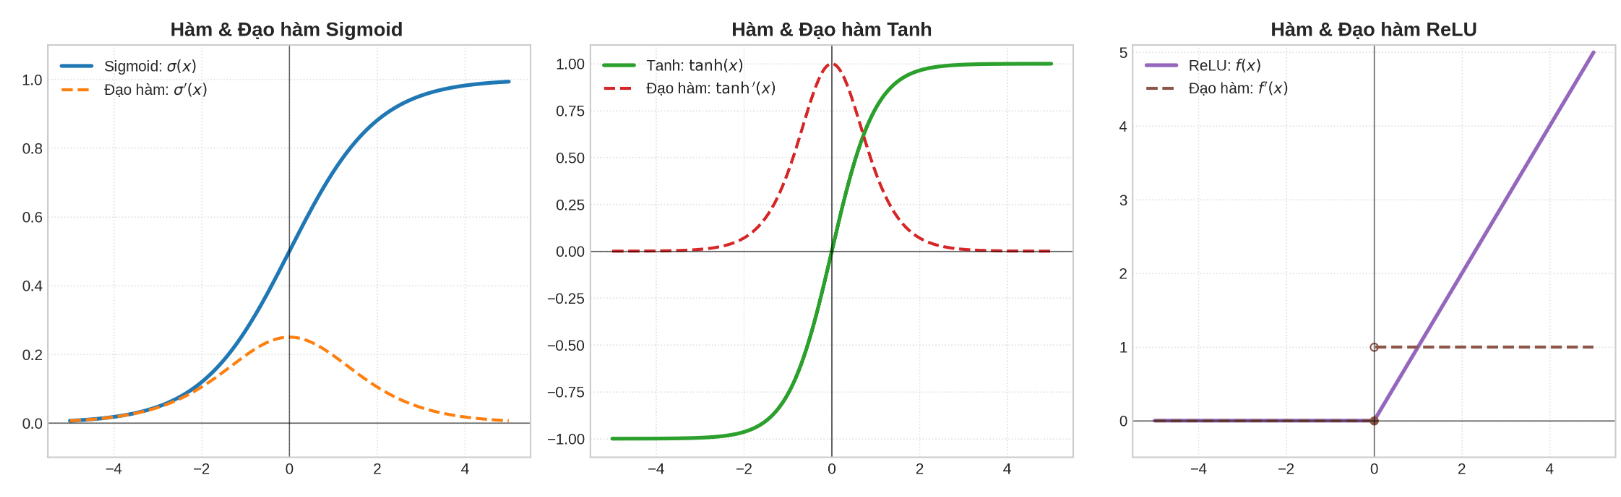
\includegraphics[width=\linewidth]{Images/04_Images/AFs.png}
    \caption{Các hàm kích hoạt Sigmoid, Tanh, ReLU và đạo hàm của chúng.}
\end{figure}

\begin{lstlisting}[caption={Mã Python cho các hàm kích hoạt ReLU, Sigmoid, Tanh và vẽ đồ thị hàm số cùng với đạo hàm của chúng.}, language=Python]
import numpy as np
import matplotlib.pyplot as plt

# 1. Dinh nghia ham kich hoat
def sigmoid(x):
    return 1 / (1 + np.exp(-x))

def sigmoid_derivative(x):
    s = sigmoid(x)
    return s * (1 - s)

def tanh(x):
    return np.tanh(x)

def tanh_derivative(x):
    return 1 - np.tanh(x)**2

def relu(x):
    return np.maximum(0, x)

# 2. Tao du lieu
x = np.linspace(-5, 5, 500)
x_neg = np.linspace(-5, 0, 250, endpoint=False) # x < 0
x_pos = np.linspace(0, 5, 250)[1:]              # x > 0

# 3. Ve do thi
fig, axes = plt.subplots(1, 3, figsize=(15, 4.5), dpi=300)

# --- Sigmoid ---
axes[0].plot(x, sigmoid(x), label=r'Sigmoid: $\sigma(x)$', color='#1f77b4', linewidth=2.5)
axes[0].plot(x, sigmoid_derivative(x), label=r"Dao ham: $\sigma'(x)$", color='#ff7f0e', linestyle='--', linewidth=2)
axes[0].set_title('Ham & Dao ham Sigmoid', fontsize=13, fontweight='bold')
axes[0].axhline(0, color='black', linewidth=0.8, alpha=0.6)
axes[0].axvline(0, color='black', linewidth=0.8, alpha=0.6)
axes[0].set_ylim(-0.1, 1.1)
axes[0].legend(loc='upper left')
axes[0].grid(True, linestyle=':', alpha=0.6)

# --- Tanh ---
axes[1].plot(x, tanh(x), label=r'Tanh: $\tanh(x)$', color='#2ca02c', linewidth=2.5)
axes[1].plot(x, tanh_derivative(x), label=r"Dao ham: $\tanh'(x)$", color='#d62728', linestyle='--', linewidth=2)
axes[1].set_title('Ham & Dao ham Tanh', fontsize=13, fontweight='bold')
axes[1].axhline(0, color='black', linewidth=0.8, alpha=0.6)
axes[1].axvline(0, color='black', linewidth=0.8, alpha=0.6)
axes[1].set_ylim(-1.1, 1.1)
axes[1].legend(loc='upper left')
axes[1].grid(True, linestyle=':', alpha=0.6)

# --- ReLU ---
axes[2].plot(x, relu(x), label=r'ReLU: $f(x)$', color='#9467bd', linewidth=2.5)
axes[2].plot(x_neg, np.zeros_like(x_neg), color='#8c564b', linestyle='--', linewidth=2, label=r"Dao ham: $f'(x)$")
axes[2].plot(x_pos, np.ones_like(x_pos), color='#8c564b', linestyle='--', linewidth=2)
axes[2].plot(0, 0, marker='o', markersize=5, color='#8c564b')
axes[2].plot(0, 1, marker='o', markersize=5, color='#8c564b', fillstyle='none')
axes[2].set_title('Ham & Dao ham ReLU', fontsize=13, fontweight='bold')
axes[2].axhline(0, color='black', linewidth=0.8, alpha=0.6)
axes[2].axvline(0, color='black', linewidth=0.8, alpha=0.6)
axes[2].set_ylim(-0.5, 5.1)
axes[2].legend(loc='upper left')
axes[2].grid(True, linestyle=':', alpha=0.6)

plt.tight_layout()
plt.savefig('activation_functions_thesis.png', dpi=300)
plt.show()
\end{lstlisting}























% \subsubsection{Sự suy biến của mạng nơ-ron tuyến tính đa tầng}

% \begin{definition}{Hàm kích hoạt đồng nhất\\}
% Toán tử kích hoạt đồng nhất $\sigma_{\mathrm{id}}: \mathbb{R} \to \mathbb{R}$ được xác định bởi ánh xạ đồng nhất trên trường số thực:
% \begin{equation}
%     \sigma_{\mathrm{id}}(z) = z, \qquad \forall z \in \mathbb{R}.
% \end{equation}
% Xét trên không gian vector đa chiều $\mathbf{z} \in \mathbb{R}^d$, toán tử vector $\boldsymbol{\sigma}_{\mathrm{id}}: \mathbb{R}^d \to \mathbb{R}^d$ tác động theo từng tọa độ chính là toán tử đồng nhất $\operatorname{id}_{\mathbb{R}^d}$, với tập ảnh: $\operatorname{Im}(\sigma_{\mathrm{id}}) = \mathbb{R}$.

% \textbf{Tính chất giải tích và đạo hàm.}
% \begin{enumerate}
%     \item \textit{Tính trơn:} Ánh xạ $\sigma_{\mathrm{id}}$ là một đẳng cấu tuyến tính và thuộc lớp hàm khả vi vô hạn $C^\infty(\mathbb{R})$.
%     \item \textit{Gradient bậc một:} Đạo hàm bậc nhất là một hằng số đơn vị trên toàn miền xác định:
%     \begin{equation}
%         \sigma_{\mathrm{id}}'(z) = 1, \qquad \forall z \in \mathbb{R}.
%     \end{equation}
%     Khi đó, ma trận Jacobian của phép biến đổi tọa độ đồng nhất là ma trận đơn vị: $\mathbf{J}_{\boldsymbol{\sigma}_{\mathrm{id}}}(\mathbf{z}) = \mathbf{I}_d$.
%     \item \textit{Sự triệt tiêu đạo hàm bậc cao:} Mọi đạo hàm cấp $k \ge 2$ đều đồng nhất bằng $0$:
%     \begin{equation}
%         \sigma_{\mathrm{id}}^{(k)}(z) = 0, \qquad \forall z \in \mathbb{R}, \quad \forall k \ge 2.
%     \end{equation}
% \end{enumerate}
% \end{definition}


% Xét một mạng nơ-ron truyền thẳng gồm $L$ lớp ẩn.
% Ký hiệu số lượng nơ-ron tại các lớp lần lượt là $n_0, n_1, \dots, n_{L+1}$, với $n_0 = d$ là số chiều đầu vào và $n_{L+1} = m$ là số chiều đầu ra.

% Tại mỗi lớp $l \in \{1, 2, \dots, L+1\}$, ma trận trọng số và véc-tơ độ lệch tương ứng được ký hiệu là $\mathbf{W}^{(l)} \in \mathbb{R}^{n_l \times n_{l-1}}$ và $\mathbf{b}^{(l)} \in \mathbb{R}^{n_l}$. Phép biến đổi affin ánh xạ từ véc-tơ kích hoạt của lớp trước $\mathbf{a}^{(l-1)}$ sang véc-tơ tiền kích hoạt của lớp hiện tại $\mathbf{z}^{(l)}$ được định nghĩa là:

% \begin{equation}
%     \mathbf{z}^{(l)} = T_l(\mathbf{a}^{(l-1)}) \triangleq \mathbf{W}^{(l)} \mathbf{a}^{(l-1)} + \mathbf{b}^{(l)},
% \end{equation}

% với quy ước $\mathbf{a}^{(0)} = \mathbf{x} \in \mathbb{R}^d$ là véc-tơ dữ liệu đầu vào. Tại mỗi lớp, véc-tơ kích hoạt đầu ra được tính bởi $\mathbf{a}^{(l)} = \sigma(\mathbf{z}^{(l)})$.

% \begin{theorem}{Sự suy biến của mạng nơ-ron tuyến tính đa tầng} \label{thm:linear_collapse}


% Giả sử tất cả $L+1$ lớp của mạng đều sử dụng hàm kích hoạt đồng nhất $\sigma_{\mathrm{id}}(z) = z$. Khi đó, hàm biểu diễn toàn cục của mạng $f: \mathbb{R}^d \to \mathbb{R}^m$ suy biến thành một phép biến đổi affine đơn tầng duy nhất:

% \begin{equation}
%     \mathbf{y} = f(\mathbf{x}) = \overline{\mathbf{W}}\mathbf{x} + \overline{\mathbf{b}}, \label{eq:collapsed_model}
% \end{equation}

% trong đó ma trận trọng số tổng hợp $\overline{\mathbf{W}} \in \mathbb{R}^{m \times d}$ và véc-tơ độ lệch tổng hợp $\overline{\mathbf{b}} \in \mathbb{R}^m$ được xác định tường minh bởi:

% \begin{align}
%     \overline{\mathbf{W}} &= \prod_{l=L+1}^{1} \mathbf{W}^{(l)} = \mathbf{W}^{(L+1)} \mathbf{W}^{(L)} \cdots \mathbf{W}^{(1)}, \label{eq:W_bar} \\
%     \overline{\mathbf{b}} &= \mathbf{b}^{(L+1)} + \sum_{i=1}^L \left( \prod_{j=L+1}^{i+1} \mathbf{W}^{(j)} \right) \mathbf{b}^{(i)}, \label{eq:b_bar}
% \end{align}

% với quy ước tích có thứ tự của các ma trận $\prod_{j=p}^{q} \mathbf{A}_j \triangleq \mathbf{A}_p \mathbf{A}_{p-1} \cdots \mathbf{A}_q$ khi $p \ge q$.
% \end{theorem}

% \begin{proof}
% Chúng ta sẽ chứng minh định lý bằng phương pháp quy nạp toán học theo số lớp $l$. Gọi $\mathbf{a}^{(l)}$ là véc-tơ đầu ra của lớp thứ $l$. Ta cần chứng minh:
% \begin{equation}
%     \mathbf{a}^{(l)} = \left( \prod_{j=l}^{1} \mathbf{W}^{(j)} \right) \mathbf{x} + \mathbf{b}^{(l)} + \sum_{i=1}^{l-1} \left( \prod_{j=l}^{i+1} \mathbf{W}^{(j)} \right) \mathbf{b}^{(i)}.
% \end{equation}

% \textbf{Cơ sở quy nạp ($l = 1$):} \\
% Do hàm kích hoạt là hàm đồng nhất, ta có:
% \begin{equation}
%     \mathbf{a}^{(1)} = \sigma_{\mathrm{id}}(\mathbf{z}^{(1)}) = \mathbf{W}^{(1)}\mathbf{a}^{(0)} + \mathbf{b}^{(1)} = \mathbf{W}^{(1)}\mathbf{x} + \mathbf{b}^{(1)}.
% \end{equation}
% Công thức đúng với $l = 1$ (tổng sigma bằng 0 theo quy ước tổng rỗng).

% \textbf{Bước quy nạp:} \\
% Giả sử công thức đúng cho lớp thứ $l = k$ ($1 \le k \le L$). Xét tại lớp thứ $k+1$:
% \begin{align*}
%     \mathbf{a}^{(k+1)} &= \sigma_{\mathrm{id}}(\mathbf{W}^{(k+1)}\mathbf{a}^{(k)} + \mathbf{b}^{(k+1)}) \\
%     &= \mathbf{W}^{(k+1)} \left[ \left( \prod_{j=k}^{1} \mathbf{W}^{(j)} \right) \mathbf{x} + \mathbf{b}^{(k)} + \sum_{i=1}^{k-1} \left( \prod_{j=k}^{i+1} \mathbf{W}^{(j)} \right) \mathbf{b}^{(i)} \right] + \mathbf{b}^{(k+1)} \\
%     &= \left( \mathbf{W}^{(k+1)} \prod_{j=k}^{1} \mathbf{W}^{(j)} \right) \mathbf{x} + \mathbf{W}^{(k+1)}\mathbf{b}^{(k)} + \sum_{i=1}^{k-1} \left( \mathbf{W}^{(k+1)} \prod_{j=k}^{i+1} \mathbf{W}^{(j)} \right) \mathbf{b}^{(i)} + \mathbf{b}^{(k+1)} \\
%     &= \left( \prod_{j=k+1}^{1} \mathbf{W}^{(j)} \right) \mathbf{x} + \mathbf{b}^{(k+1)} + \sum_{i=1}^{k} \left( \prod_{j=k+1}^{i+1} \mathbf{W}^{(j)} \right) \mathbf{b}^{(i)}.
% \end{align*}
% Theo nguyên lý quy nạp, công thức đúng với mọi $l \in \{1, \dots, L+1\}$. 
% Thay $l = L+1$ và đặt $\mathbf{y} = \mathbf{a}^{(L+1)}$, ta thu được chính xác kết quả của các phương trình \eqref{eq:W_bar} và \eqref{eq:b_bar}.
% \end{proof}


% \begin{proof}

% Vì $\sigma_{\mathrm{id}}$ là ánh xạ đồng nhất, vector kích hoạt tại mỗi tầng $l \in \{1, \dots, L+1\}$ thỏa $\mathbf{a}^{(l)} = \sigma_{\mathrm{id}}(\mathbf{z}^{(l)}) = \mathbf{z}^{(l)}$. Do đó, toàn bộ mạng tương đương với phép hợp thành liên tiếp của $L+1$ ánh xạ affine:

% \begin{equation}
%     \mathbf{y} = \mathbf{a}^{(L+1)} = (T_{L+1} \circ T_L \circ \dots \circ T_1)(\mathbf{x}).
% \end{equation}

% \textbf{Trường hợp 1: Mô hình thuần nhất không có độ lệch ($\mathbf{b}^{(l)} = \mathbf{0}, \forall l$).} \\
% Ta tiến hành chứng minh bằng quy nạp toán học theo số lớp $l$. 
% \begin{itemize}
%     \item \textit{Cơ sở quy nạp ($l = 1$):} $\mathbf{a}^{(1)} = \mathbf{W}^{(1)}\mathbf{x}$, mệnh đề hiển nhiên đúng.
%     \item \textit{Bước quy nạp:} Giả sử mệnh đề đúng đến lớp $p \le L$, nghĩa là:
%     \begin{equation}
%         \mathbf{a}^{(p)} = \left(\mathbf{W}^{(p)} \mathbf{W}^{(p-1)} \cdots \mathbf{W}^{(1)}\right) \mathbf{x}.
%     \end{equation}
%     Xét lớp $p+1$, theo tính kết hợp của phép nhân ma trận:
%     \begin{align}
%         \mathbf{a}^{(p+1)} &= \mathbf{W}^{(p+1)} \mathbf{a}^{(p)} \nonumber \\
%         &= \mathbf{W}^{(p+1)} \left[ \left(\mathbf{W}^{(p)} \mathbf{W}^{(p-1)} \cdots \mathbf{W}^{(1)}\right) \mathbf{x} \right] \nonumber \\
%         &= \left(\mathbf{W}^{(p+1)} \mathbf{W}^{(p)} \cdots \mathbf{W}^{(1)}\right) \mathbf{x}.
%     \end{align}
% \end{itemize}
% Theo nguyên lý quy nạp, tại lớp đầu ra $l = L+1$:
% \begin{equation}
%     \mathbf{y} = \mathbf{a}^{(L+1)} = \left(\prod_{j=L+1}^{1} \mathbf{W}^{(j)}\right) \mathbf{x} = \overline{\mathbf{W}}\mathbf{x}.
% \end{equation}

% \textbf{Trường hợp 2: Mô hình tổng quát có độ lệch ($\mathbf{b}^{(l)} \neq \mathbf{0}$).} \\
% Ta chứng minh công thức tổng quát của vector kích hoạt tại lớp  $k \in \{1, \dots, L+1\}$ bằng quy nạp:
% \begin{equation}
%     \mathbf{a}^{(k)} = \left( \prod_{j=k}^1 \mathbf{W}^{(j)} \right) \mathbf{x} + \mathbf{b}^{(k)} + \sum_{i=1}^{k-1} \left( \prod_{j=k}^{i+1} \mathbf{W}^{(j)} \right) \mathbf{b}^{(i)}. \tag{$*$}
% \end{equation}
% \begin{itemize}
%     \item \textit{Cơ sở quy nạp ($k = 1$):} 
%     $\mathbf{a}^{(1)} = \mathbf{W}^{(1)}\mathbf{x} + \mathbf{b}^{(1)}$. ($*$) đúng (tổng rỗng quy ước bằng $\mathbf{0}$).
%     \item \textit{Bước quy nạp:} Giả sử ($*$) đúng với $k = p \le L$. Tại lớp $p+1$:
%     \begin{align}
%         \mathbf{a}^{(p+1)} &= \mathbf{W}^{(p+1)} \mathbf{a}^{(p)} + \mathbf{b}^{(p+1)} \nonumber \\
%         &= \mathbf{W}^{(p+1)} \left[ \left( \prod_{j=p}^1 \mathbf{W}^{(j)} \right) \mathbf{x} + \mathbf{b}^{(p)} + \sum_{i=1}^{p-1} \left( \prod_{j=p}^{i+1} \mathbf{W}^{(j)} \right) \mathbf{b}^{(i)} \right] + \mathbf{b}^{(p+1)} \nonumber \\
%         &= \left( \mathbf{W}^{(p+1)} \prod_{j=p}^1 \mathbf{W}^{(j)} \right) \mathbf{x} + \mathbf{b}^{(p+1)} + \mathbf{W}^{(p+1)}\mathbf{b}^{(p)} + \sum_{i=1}^{p-1} \left( \mathbf{W}^{(p+1)} \prod_{j=p}^{i+1} \mathbf{W}^{(j)} \right) \mathbf{b}^{(i)} \nonumber \\
%         &= \left( \prod_{j=p+1}^1 \mathbf{W}^{(j)} \right) \mathbf{x} + \mathbf{b}^{(p+1)} + \sum_{i=1}^p \left( \prod_{j=p+1}^{i+1} \mathbf{W}^{(j)} \right) \mathbf{b}^{(i)}.
%     \end{align}
% \end{itemize}
% Như vậy, công thức ($*$) đúng với $k = p+1$. Đặt $k = L+1$, ta thu được chính xác biểu thức \eqref{eq:collapsed_model} với $\overline{\mathbf{W}}$ và $\overline{\mathbf{b}}$ cho bởi \eqref{eq:W_bar} và \eqref{eq:b_bar}. 
% \end{proof}

% % Từ Định lý \ref{thm:linear_collapse}, chúng ta có thể rút ra các tính chất đại số nền tảng và giới hạn nghiêm ngặt về dung lượng biểu diễn của các kiến trúc mạng không có hàm kích hoạt phi tuyến.

% \begin{remark}{Tính khép kín của phép hợp thành affine}

% Trong không gian các ánh xạ affine, phép toán hàm hợp có tính khép kín. Cụ thể, nếu $T_1: \mathbb{R}^p \to \mathbb{R}^q$ và $T_2: \mathbb{R}^q \to \mathbb{R}^r$ là các biến đổi affin, thì ánh xạ hợp thành $T_2 \circ T_1: \mathbb{R}^p \to \mathbb{R}^r$ cũng là một biến đổi affine. 
% Bản chất của Định lý \ref{thm:linear_collapse} chính là hệ quả của tính chất đại số cơ bản này khi áp dụng liên tiếp trên $L+1$ lớp.
% \end{remark}

% Kết quả này cho thấy việc tăng độ sâu của mạng không đem lại bất kỳ khả năng nội suy nào phức tạp hơn cho mô hình tuyến tính truyền thống. 

% % Thậm chí, khi kết hợp với cấu trúc phân loại ở lớp cuối, mạng suy biến về cấu trúc tối giản nhất:

% % \begin{corollary}{Sự suy biến về mô hình Perceptron đơn tầng}
% % \label{cor:perceptron_collapse}

% % Xét một mạng nơ-ron đa tầng với hàm kích hoạt đồng nhất tại tất cả các tầng ẩn. Tầng đầu ra gồm một nơ-ron duy nhất sử dụng hàm kích hoạt dấu $\mathrm{sgn}(\cdot)$ để thực hiện bài toán phân loại nhị phân. Giá trị dự đoán được tính bởi:
% % \begin{equation}
% %     \hat{y} = \mathrm{sgn}\left(\mathbf{w}^{(L+1)\top} \mathbf{a}^{(L)} + b^{(L+1)}\right).
% % \end{equation}
% % Khi đó, toàn bộ kiến trúc mạng biểu diễn chính xác một mô hình Perceptron đơn tầng (Rosenblatt Perceptron):
% % \begin{equation}
% %     \hat{y} = \mathrm{sgn}\left(\overline{\mathbf{w}}^\top \mathbf{x} + \overline{b}\right),
% % \end{equation}
% % trong đó vector trọng số tổng hợp $\overline{\mathbf{w}}^\top = \mathbf{w}^{(L+1)\top} \prod_{j=L}^1 \mathbf{W}^{(j)} \in \mathbb{R}^{1 \times d}$ và $\overline{b} \in \mathbb{R}$ được tính theo phương trình \eqref{eq:b_bar}.
% % \end{corollary}

% % Nghiêm trọng hơn việc không thể học được các mặt phân định phi tuyến, mạng nơ-ron tuyến tính đa tầng còn phải đối mặt với hiện tượng mất mát thông tin không thể phục hồi do cấu trúc hạng của ma trận.

% % \begin{corollary}{Giới hạn dung lượng biểu diễn do hiện tượng thắt nút cổ chai}

% % \label{cor:rank_bottleneck}
% % Giả sử bỏ qua các vector độ lệch $\mathbf{b}$ để đơn giản hóa, phép biến đổi tổng hợp của mạng là $\mathbf{y} = \overline{\mathbf{W}}\mathbf{x}$. Theo tính chất của hạng ma trận đối với phép nhân, ta luôn có:
% % \begin{equation}
% %     \mathrm{rank}(\overline{\mathbf{W}}) = \mathrm{rank}\left(\prod_{l=L+1}^1 \mathbf{W}^{(l)}\right) \le \min_{1 \le l \le L+1} \{ \mathrm{rank}(\mathbf{W}^{(l)}) \} \le \min_{0 \le l \le L+1} \{n_l\}. \label{eq:rank_bottleneck}
% % \end{equation}
% % \end{corollary}

% % Phương trình \eqref{eq:rank_bottleneck} chỉ ra một giới hạn cứng: Nếu tồn tại bất kỳ tầng ẩn $l$ nào có số lượng nơ-ron $n_l < \min(d, m)$, ma trận tham số tổng hợp $\overline{\mathbf{W}}$ sẽ trở thành ma trận suy biến. Cấu trúc này tạo ra một \emph{nút thắt cổ chai thông tin}, ép toàn bộ dữ liệu đầu vào phải chiếu qua một không gian con affin có số chiều nhỏ hơn, dẫn đến sự phá hủy thông tin không thể đảo ngược. Trái lại, khi sử dụng các hàm kích hoạt phi tuyến $\sigma$ (như ReLU, Tanh), mạng nơ-ron có thể phá vỡ ràng buộc về không gian con tuyến tính này, bảo toàn thông tin chiều cao và ánh xạ dữ liệu lên các đa tạp phi tuyến phức tạp.



\subsection{Mạng Nơ-ron Sâu}
\subsubsection{Mạng nơ-ron nông và mạng nơ-ron sâu}
Dựa trên số lượng lớp trong kiến trúc, mạng nơ-ron có thể phân loại thành: \emph{mạng nơ-ron nông} và \emph{mạng nơ-ron sâu} \cite{aalto_neural_networks}. Thuật ngữ \emph{nông} và \emph{sâu} chủ yếu mô tả độ sâu của kiến trúc, tức số lượng lớp của mạng. Mạng nơ-ron nông thường chỉ có một lớp ẩn, trong khi mạng nơ-ron sâu có nhiều lớp ẩn nối tiếp với nhau.

Đối với mạng nơ-ron nông, do có ít lớp ẩn nên kiến trúc có độ phức tạp thấp và thường thuận lợi đối với các bài toán có quy mô hoặc cấu trúc không quá phức tạp. Tuy nhiên, khả năng biểu diễn của mạng không chỉ phụ thuộc vào số lượng lớp mà còn phụ thuộc vào số lượng nơ-ron trong một lớp, hàm kích hoạt và số lượng tham số. Vì vậy, không nên đồng nhất mạng nơ-ron nông với mô hình có năng lực biểu diễn thấp trong mọi trường hợp.

\begin{figure}[H]
    \centering
    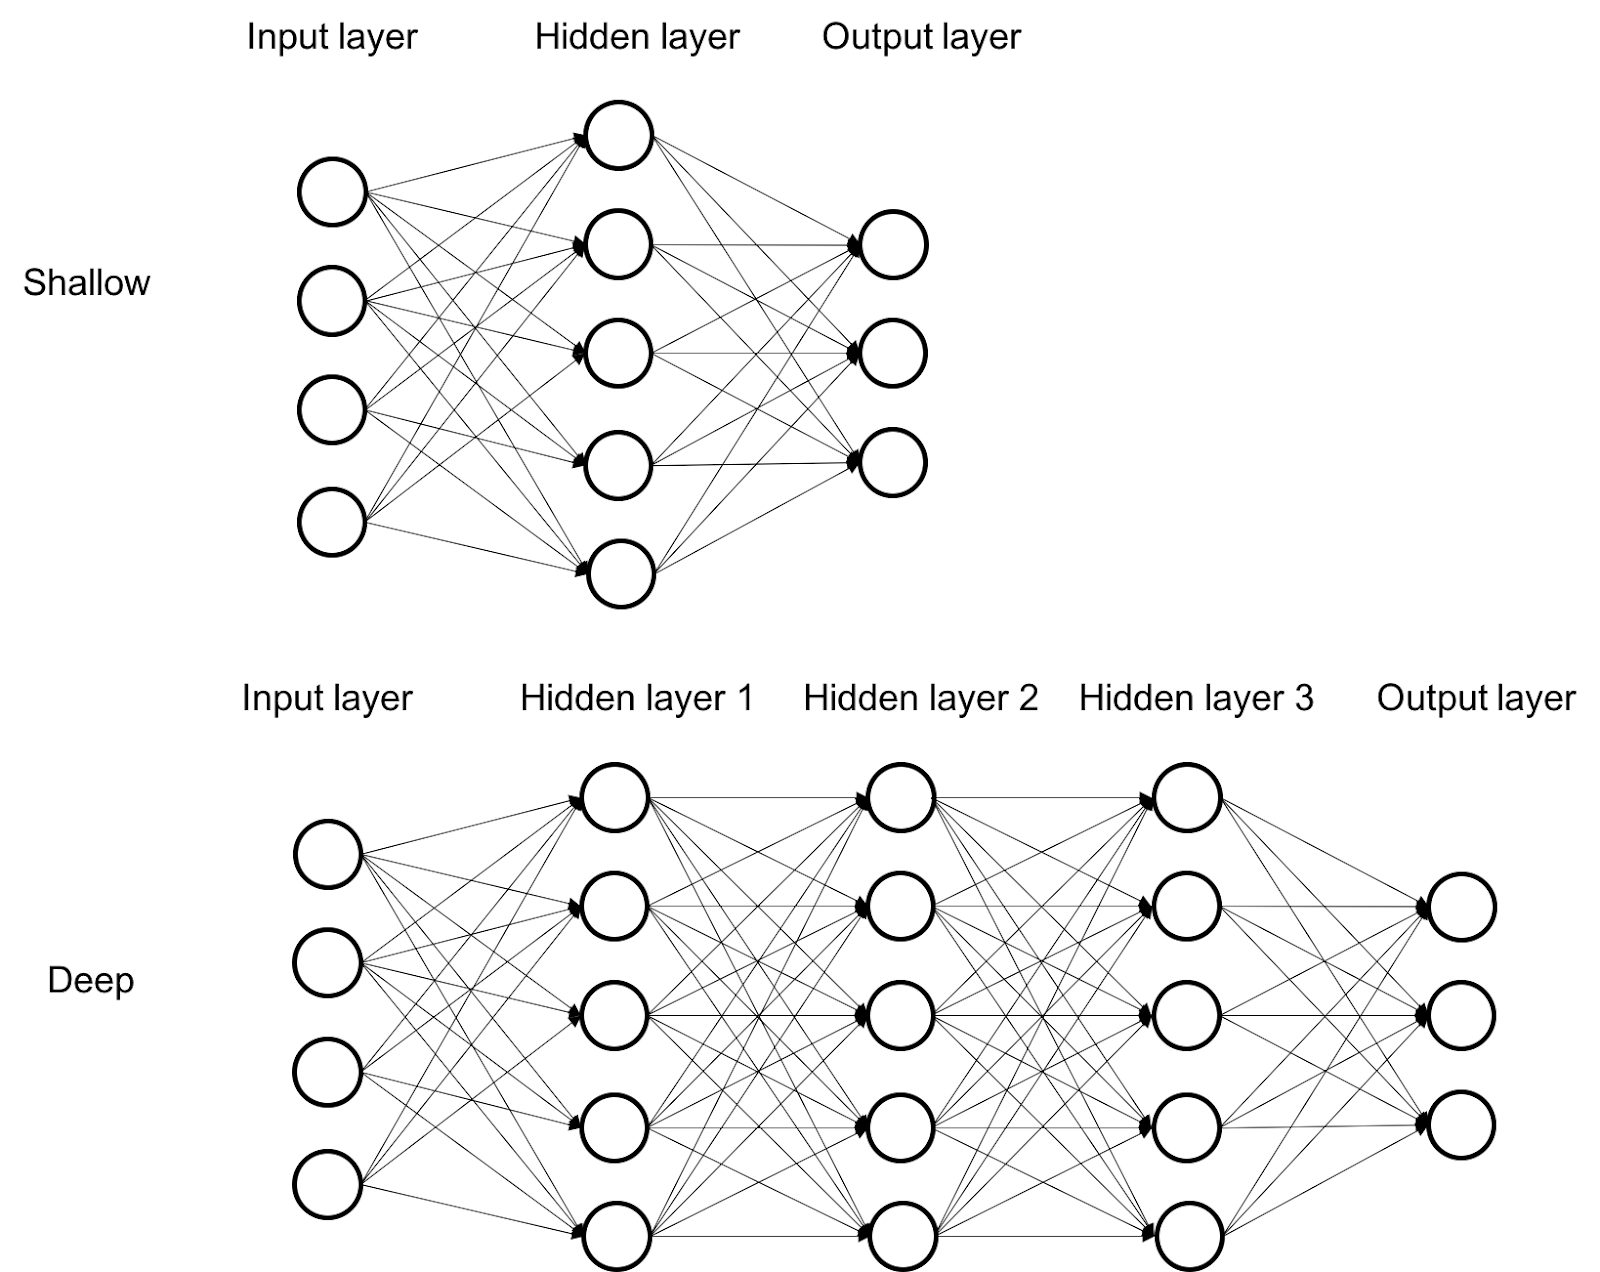
\includegraphics[width=0.8\linewidth]{Images/04_Images/shallow&deep_nn.png}
    \caption{Mạng nơ-ron nông và mạng nơ-ron sâu}
\end{figure}

Đối với mạng nơ-ron sâu, nhiều lớp ẩn được sử dụng để xây dựng một chuỗi các biểu diễn trung gian. Trong nhiều kiến trúc, các lớp ở những vị trí khác nhau có thể học các mức độ biểu diễn khác nhau: các lớp gần đầu vào thường mã hóa những đặc trưng có quan hệ trực tiếp hơn với dữ liệu ban đầu, trong khi các lớp sâu hơn có khả năng kết hợp các biểu diễn trước đó để hình thành những đặc trưng có mức độ trừu tượng cao hơn. Cấu trúc biểu diễn phân cấp này cho phép mạng mô hình hóa các quan hệ phức tạp thông qua nhiều phép biến đổi được hợp thành, và là một đặc điểm quan trọng của học sâu.

Tuy nhiên, việc gia tăng chiều sâu cũng làm tăng độ phức tạp của quá trình tính toán và tối ưu hóa. Trong lan truyền ngược của các mạng sâu, quá trình lan truyền gradient của hàm mất mát đối với các tham số của mạng qua nhiều lớp liên tiếp có thể dẫn đến hiện tượng suy giảm hoặc bùng nổ gradient, gây khó khăn cho quá trình huấn luyện. Những tiến bộ về kiến trúc mạng, hàm kích hoạt, thuật toán tối ưu, kỹ thuật khởi tạo tham số, chuẩn hóa và phần cứng tính toán song song đã góp phần khắc phục các hạn chế này, qua đó cho phép huấn luyện các mô hình học sâu với quy mô ngày càng lớn.

\subsubsection{Lan truyền tiến}
Về cơ bản quy trình huấn luyện mạng nơ-ron truyền thẳng gồm hai pha tuần tự: 
\begin{enumerate}
    \item \textit{Lan truyền tiến:} Dữ liệu đầu vào được truyền một chiều qua các lớp ẩn đến lớp đầu ra để tạo giá trị dự đoán.
    
    \item \textit{Lan truyền ngược:} Đánh giá mức độ sai lệch giữa giá trị dự đoán và giá trị thực tế thông qua hàm mất mát, từ đó áp dụng quy tắc chuỗi để tính các gradient của hàm mất mát theo từng tham số ngược từ lớp đầu ra về lớp đầu vào.
\end{enumerate}

Nhằm đảm bảo tính nhất quán trong ký hiệu toán học xuyên suốt mạng nơ-ron, véc-tơ đặc trưng đầu vào được quy ước là véc-tơ kích hoạt của lớp $0$, ký hiệu là $\mathbf{a}^{[0]} \in \mathbb{R}^{n_0}$:
\begin{equation}
    \mathbf{a}^{[0]} = \begin{bmatrix} a_1^{[0]} & a_2^{[0]} & \dots & a_{n_0}^{[0]} \end{bmatrix}^\top,
\end{equation}
trong đó $n_0$ là số lượng chiều (đặc trưng) của dữ liệu đầu vào.

Giả sử mạng nơ-ron truyền thẳng bao gồm $L$ lớp (không tính lớp đầu vào $l=0$), trong đó mỗi lớp thứ $l$ (với $1 \le l \le L$) chứa $n_l$ nơ-ron. Lớp cuối cùng $L$ được gọi là lớp đầu ra. Tại một lớp $l$ bất kỳ, ta định nghĩa các đại lượng không gian tham số như sau:
\begin{equation}
\begin{aligned}
    \mathbf{W}^{[l]} &= \begin{bmatrix}
        w_{11}^{[l]} & w_{12}^{[l]} & \dots & w_{1, n_{l-1}}^{[l]} \\
        w_{21}^{[l]} & w_{22}^{[l]} & \dots & w_{2, n_{l-1}}^{[l]} \\
        \vdots & \vdots & \ddots & \vdots \\
        w_{n_l 1}^{[l]} & w_{n_l 2}^{[l]} & \dots & w_{n_l, n_{l-1}}^{[l]}
    \end{bmatrix} \in \mathbb{R}^{n_l \times n_{l-1}}, \\
    \mathbf{a}^{[l]} &= \begin{bmatrix} a_1^{[l]} \\ a_2^{[l]} \\ \vdots \\ a_{n_l}^{[l]} \end{bmatrix} \in \mathbb{R}^{n_l}, \quad
    \mathbf{b}^{[l]} = \begin{bmatrix} b_1^{[l]} \\ b_2^{[l]} \\ \vdots \\ b_{n_l}^{[l]} \end{bmatrix} \in \mathbb{R}^{n_l}.
\end{aligned}
\end{equation}
Trong đó:
\begin{itemize}
    \item $l$: Biến chỉ số biểu diễn thứ tự của lớp đang xét, $l \in \{1, 2, \dots, L\}$.
    \item $n_l$: Số lượng đơn vị tính toán tại lớp thứ $l$. Tương ứng, $n_{l-1}$ là số lượng đơn vị tại lớp liền trước.
    \item Chỉ số trên ngoặc vuông $[l]$: Quy ước chỉ số thứ tự của lớp tính toán trong mạng nơ-ron. Ở đây, $[0]$ biểu thị lớp đầu vào.
    \item $\mathbf{W}^{[l]}$: Ma trận trọng số kết nối từ lớp $l-1$ sang lớp $l$.
    \item $w_{ij}^{[l]}$: Phần tử nằm trên hàng $i$, cột $j$ của ma trận $\mathbf{W}^{[l]}$. Giá trị này định lượng mức độ ảnh hưởng (trọng số liên kết) của tín hiệu từ nơ-ron thứ $j$ thuộc lớp $l-1$ truyền tới nơ-ron thứ $i$ thuộc lớp $l$.
    \item $\mathbf{a}^{[l]}$: Véc-tơ kích hoạt (đầu ra) của lớp $l$.
    \item $\mathbf{b}^{[l]}$: Véc-tơ độ chệch của lớp $l$.
    \item $b_i^{[l]}$: Hệ số độ chệch tương ứng với nơ-ron thứ $i$ tại lớp $l$.
\end{itemize}
Tại mỗi lớp $l$, quá trình lan truyền tiến được mô tả qua hai bước. Đầu tiên, véc-tơ tiền kích hoạt $\mathbf{z}^{[l]}$ được tính thông qua một phép biến đổi tuyến tính:
\begin{equation}
    \mathbf{z}^{[l]} = \mathbf{W}^{[l]} \mathbf{a}^{[l-1]} + \mathbf{b}^{[l]}
\end{equation}
Sau đó, véc-tơ kích hoạt $\mathbf{a}^{[l]}$ được tính bằng cách áp dụng một hàm kích hoạt $\sigma^{[l]}$ lên véc-tơ $\mathbf{z}^{[l]}$:
\begin{equation}
    \mathbf{a}^{[l]} = \sigma^{[l]}(\mathbf{z}^{[l]})
\end{equation}
Trong đó, $\sigma^{[l]}(\cdot)$ là hàm kích hoạt của lớp $l$, tác động độc lập theo từng phần tử lên thành phần đầu vào của nó.

Để làm rõ bản chất đại số, ta khai triển chi tiết phép tính cho véc-tơ tiền kích hoạt $\mathbf{z}^{[l]}$:
\begin{equation}
\begin{aligned}
    \mathbf{z}^{[l]} &= \mathbf{W}^{[l]} \mathbf{a}^{[l-1]} + \mathbf{b}^{[l]} \\
    &= \begin{bmatrix}
        w_{11}^{[l]} & w_{12}^{[l]} & \dots & w_{1, n_{l-1}}^{[l]} \\
        w_{21}^{[l]} & w_{22}^{[l]} & \dots & w_{2, n_{l-1}}^{[l]} \\
        \vdots & \vdots & \ddots & \vdots \\
        w_{n_l 1}^{[l]} & w_{n_l 2}^{[l]} & \dots & w_{n_l, n_{l-1}}^{[l]}
    \end{bmatrix}
    \begin{bmatrix}
        a_1^{[l-1]} \\
        a_2^{[l-1]} \\
        \vdots \\
        a_{n_{l-1}}^{[l-1]}
    \end{bmatrix}
    +
    \begin{bmatrix}
        b_1^{[l]} \\
        b_2^{[l]} \\
        \vdots \\
        b_{n_l}^{[l]}
    \end{bmatrix} \\
    &= \begin{bmatrix}
        w_{11}^{[l]} a_1^{[l-1]} + \dots + w_{1, n_{l-1}}^{[l]} a_{n_{l-1}}^{[l-1]} + b_1^{[l]} \\
        w_{21}^{[l]} a_1^{[l-1]} + \dots + w_{2, n_{l-1}}^{[l]} a_{n_{l-1}}^{[l-1]} + b_2^{[l]} \\
        \vdots \\
        w_{n_l 1}^{[l]} a_1^{[l-1]} + \dots + w_{n_l, n_{l-1}}^{[l]} a_{n_{l-1}}^{[l-1]} + b_{n_l}^{[l]}
    \end{bmatrix} \\
    &= \begin{bmatrix}
        \sum_{j=1}^{n_{l-1}} w_{1j}^{[l]} a_j^{[l-1]} + b_1^{[l]} \\
        \sum_{j=1}^{n_{l-1}} w_{2j}^{[l]} a_j^{[l-1]} + b_2^{[l]} \\
        \vdots \\
        \sum_{j=1}^{n_{l-1}} w_{n_l j}^{[l]} a_j^{[l-1]} + b_{n_l}^{[l]}
    \end{bmatrix}
    = \begin{bmatrix}
        z_1^{[l]} \\
        z_2^{[l]} \\
        \vdots \\
        z_{n_l}^{[l]}
    \end{bmatrix}
\end{aligned}
\label{f-z}
\end{equation}
Véc-tơ kích hoạt tương ứng được tính bằng cách áp dụng hàm kích hoạt lên từng phần tử của véc-tơ tiền kích hoạt:
\begin{equation}
\begin{aligned}
    \mathbf{a}^{[l]} &= \sigma^{[l]}(\mathbf{z}^{[l]}) \\
    &= \begin{bmatrix}
        \sigma^{[l]}\left(z_1^{[l]}\right) \\
        \sigma^{[l]}\left(z_2^{[l]}\right) \\
        \vdots \\
        \sigma^{[l]}\left(z_{n_l}^{[l]}\right)
    \end{bmatrix}
    = \begin{bmatrix}
        a_1^{[l]} \\
        a_2^{[l]} \\
        \vdots \\
        a_{n_l}^{[l]}
    \end{bmatrix}.
\end{aligned}
\end{equation}
Nhằm tinh gọn việc biểu diễn không gian tham số, mỗi hệ số độ chệch $b_i^{[l]}$ ở lớp $l$ được quy ước đóng vai trò như một trọng số liên kết ứng với đơn vị đầu vào thứ $0$ của ma trận trọng số tại lớp $l$, ký hiệu là $w_{i0}^{[l]}$. Dưới góc độ này, véc-tơ độ chệch $\mathbf{b}^{[l]}$ tại lớp $l$ được đồng nhất hoàn toàn với véc-tơ trọng số $\mathbf{w}_0^{[l]}$:
\begin{equation}
    \mathbf{b}^{[l]} = \mathbf{w}_0^{[l]} = \begin{bmatrix} 
        w_{10}^{[l]} \\ 
        w_{20}^{[l]} \\ 
        \vdots \\ 
        w_{n_l 0}^{[l]} 
    \end{bmatrix} \in \mathbb{R}^{n_l}.
\end{equation}
\begin{figure}[H]
    \centering
    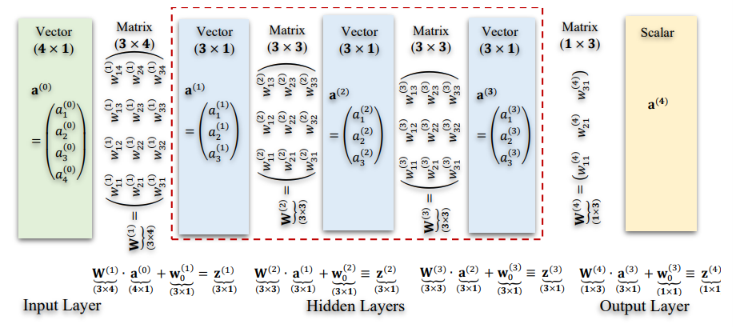
\includegraphics[width=\linewidth]{Images/04_Images/5.png}
    \caption{Kiến trúc cơ bản của một mạng nơ-ron truyền thẳng đa tầng}
    \label{4.5}
\end{figure}
Để minh họa quá trình lan truyền tiến một cách cụ thể, xét mạng nơ-ron truyền thẳng được trình bày trong Hình~\ref{4.5}, với cấu trúc $L = 4$ lớp, trong đó số lượng nơ-ron tại các lớp lần lượt là $n_0 = 4$, $n_1 = 3$, $n_2 = 3$, $n_3 = 3$ và $n_4 = 1$. Dựa trên cấu trúc này, quá trình lan truyền tiến qua từng lớp được biểu diễn như sau:
\paragraph{Lớp ẩn thứ nhất ($l = 1$)\\} 
\textbf{1. Tính véc-tơ tiền kích hoạt $\mathbf{z}^{[1]}$}
\begin{equation}
    \mathbf{z}^{[1]} = \mathbf{W}^{[1]} \mathbf{a}^{[0]} + \mathbf{w}_0^{[1]}
\end{equation}
Thay các ma trận trọng số và véc-tơ đầu vào, độ chệch cụ thể:
\begin{align}
    \begin{bmatrix} z_1^{[1]} \\ z_2^{[1]} \\ z_3^{[1]} \end{bmatrix} 
    &= \begin{bmatrix} 
        w_{11}^{[1]} & w_{12}^{[1]} & w_{13}^{[1]} & w_{14}^{[1]} \\ 
        w_{21}^{[1]} & w_{22}^{[1]} & w_{23}^{[1]} & w_{24}^{[1]} \\ 
        w_{31}^{[1]} & w_{32}^{[1]} & w_{33}^{[1]} & w_{34}^{[1]} 
    \end{bmatrix}
    \begin{bmatrix} a_1^{[0]} \\ a_2^{[0]} \\ a_3^{[0]} \\ a_4^{[0]} \end{bmatrix} 
    + \begin{bmatrix} w_{10}^{[1]} \\ w_{20}^{[1]} \\ w_{30}^{[1]} \end{bmatrix} \nonumber \\
    &= \begin{bmatrix}
        w_{11}^{[1]} a_1^{[0]} + w_{12}^{[1]} a_2^{[0]} + w_{13}^{[1]} a_3^{[0]} + w_{14}^{[1]} a_4^{[0]} \\
        w_{21}^{[1]} a_1^{[0]} + w_{22}^{[1]} a_2^{[0]} + w_{23}^{[1]} a_3^{[0]} + w_{24}^{[1]} a_4^{[0]} \\
        w_{31}^{[1]} a_1^{[0]} + w_{32}^{[1]} a_2^{[0]} + w_{33}^{[1]} a_3^{[0]} + w_{34}^{[1]} a_4^{[0]}
    \end{bmatrix}
    + \begin{bmatrix} w_{10}^{[1]} \\ w_{20}^{[1]} \\ w_{30}^{[1]} \end{bmatrix} \nonumber \\
    &= \begin{bmatrix} 
        w_{11}^{[1]} a_1^{[0]} + w_{12}^{[1]} a_2^{[0]} + w_{13}^{[1]} a_3^{[0]} + w_{14}^{[1]} a_4^{[0]} + w_{10}^{[1]} \\
        w_{21}^{[1]} a_1^{[0]} + w_{22}^{[1]} a_2^{[0]} + w_{23}^{[1]} a_3^{[0]} + w_{24}^{[1]} a_4^{[0]} + w_{20}^{[1]} \\
        w_{31}^{[1]} a_1^{[0]} + w_{32}^{[1]} a_2^{[0]} + w_{33}^{[1]} a_3^{[0]} + w_{34}^{[1]} a_4^{[0]} + w_{30}^{[1]} 
    \end{bmatrix}
\end{align}
\subparagraph{2. Tính véc-tơ kích hoạt đầu ra $\mathbf{a}^{[1]}$\\}
Áp dụng hàm kích hoạt phi tuyến $\sigma^{[1]}$ theo từng phần tử lên véc-tơ tiền kích hoạt:
\begin{equation}
    \mathbf{a}^{[1]} = \sigma^{[1]}\left(\mathbf{z}^{[1]}\right) 
    = \begin{bmatrix} a_1^{[1]} \\ a_2^{[1]} \\ a_3^{[1]} \end{bmatrix} 
    = \begin{bmatrix} 
        \sigma^{[1]}\left(z_1^{[1]}\right) \\ 
        \sigma^{[1]}\left(z_2^{[1]}\right) \\ 
        \sigma^{[1]}\left(z_3^{[1]}\right) 
    \end{bmatrix} \in \mathbb{R}^3
\end{equation}
Khai triển tường minh bằng cách thế trực tiếp các biểu thức $z_i^{[1]}$ vào hàm kích hoạt:
\begin{equation}
    \mathbf{a}^{[1]} = \begin{bmatrix} 
        \sigma^{[1]}\left( w_{11}^{[1]} a_1^{[0]} + w_{12}^{[1]} a_2^{[0]} + w_{13}^{[1]} a_3^{[0]} + w_{14}^{[1]} a_4^{[0]} + w_{10}^{[1]} \right) \\
        \sigma^{[1]}\left( w_{21}^{[1]} a_1^{[0]} + w_{22}^{[1]} a_2^{[0]} + w_{23}^{[1]} a_3^{[0]} + w_{24}^{[1]} a_4^{[0]} + w_{20}^{[1]} \right) \\
        \sigma^{[1]}\left( w_{31}^{[1]} a_1^{[0]} + w_{32}^{[1]} a_2^{[0]} + w_{33}^{[1]} a_3^{[0]} + w_{34}^{[1]} a_4^{[0]} + w_{30}^{[1]} \right)
    \end{bmatrix}
\end{equation}
Tương ứng với từng giá trị kích hoạt vô hướng:
\begin{equation}
    a_i^{[1]} = \sigma^{[1]}\left( \sum_{j=1}^{4} w_{ij}^{[1]} a_j^{[0]} + w_{i0}^{[1]} \right), \quad \forall i \in \{1, 2, 3\}.
\end{equation}

\paragraph{Lớp ẩn thứ hai ($l = 2$)\\} 
\textbf{1. Tính véc-tơ tiền kích hoạt $\mathbf{z}^{[2]}$}
\begin{equation}
    \mathbf{z}^{[2]} = \mathbf{W}^{[2]} \mathbf{a}^{[1]} + \mathbf{w}_0^{[2]}
\end{equation}
Thế các phần tử cụ thể của ma trận trọng số $\mathbf{W}^{[2]} \in \mathbb{R}^{3 \times 3}$, véc-tơ kích hoạt $\mathbf{a}^{[1]} \in \mathbb{R}^3$ từ lớp $l=1$, và véc-tơ độ chệch $\mathbf{w}_0^{[2]} \in \mathbb{R}^3$:
\begin{align}
    \begin{bmatrix} z_1^{[2]} \\ z_2^{[2]} \\ z_3^{[2]} \end{bmatrix} 
    &= \begin{bmatrix} 
        w_{11}^{[2]} & w_{12}^{[2]} & w_{13}^{[2]} \\ 
        w_{21}^{[2]} & w_{22}^{[2]} & w_{23}^{[2]} \\ 
        w_{31}^{[2]} & w_{32}^{[2]} & w_{33}^{[2]} 
    \end{bmatrix}
    \begin{bmatrix} a_1^{[1]} \\ a_2^{[1]} \\ a_3^{[1]} \end{bmatrix} 
    + \begin{bmatrix} w_{10}^{[2]} \\ w_{20}^{[2]} \\ w_{30}^{[2]} \end{bmatrix} \nonumber \\
    &= \begin{bmatrix}
        w_{11}^{[2]} a_1^{[1]} + w_{12}^{[2]} a_2^{[1]} + w_{13}^{[2]} a_3^{[1]} \\
        w_{21}^{[2]} a_1^{[1]} + w_{22}^{[2]} a_2^{[1]} + w_{23}^{[2]} a_3^{[1]} \\
        w_{31}^{[2]} a_1^{[1]} + w_{32}^{[2]} a_2^{[1]} + w_{33}^{[2]} a_3^{[1]}
    \end{bmatrix}
    + \begin{bmatrix} w_{10}^{[2]} \\ w_{20}^{[2]} \\ w_{30}^{[2]} \end{bmatrix} \nonumber \\
    &= \begin{bmatrix} 
        w_{11}^{[2]} a_1^{[1]} + w_{12}^{[2]} a_2^{[1]} + w_{13}^{[2]} a_3^{[1]} + w_{10}^{[2]} \\
        w_{21}^{[2]} a_1^{[1]} + w_{22}^{[2]} a_2^{[1]} + w_{23}^{[2]} a_3^{[1]} + w_{20}^{[2]} \\
        w_{31}^{[2]} a_1^{[1]} + w_{32}^{[2]} a_2^{[1]} + w_{33}^{[2]} a_3^{[1]} + w_{30}^{[2]} 
    \end{bmatrix}
\end{align}
\subparagraph{2. Tính véc-tơ kích hoạt đầu ra $\mathbf{a}^{[2]}$\\}
Áp dụng hàm kích hoạt phi tuyến $\sigma^{[2]}$ theo từng phần tử lên véc-tơ tiền kích hoạt $\mathbf{z}^{[2]}$:
\begin{equation}
    \mathbf{a}^{[2]} = \sigma^{[2]}\left(\mathbf{z}^{[2]}\right) 
    = \begin{bmatrix} a_1^{[2]} \\ a_2^{[2]} \\ a_3^{[2]} \end{bmatrix} 
    = \begin{bmatrix} 
        \sigma^{[2]}\left(z_1^{[2]}\right) \\ 
        \sigma^{[2]}\left(z_2^{[2]}\right) \\ 
        \sigma^{[2]}\left(z_3^{[2]}\right) 
    \end{bmatrix} \in \mathbb{R}^3
\end{equation}

Khai triển tường minh bằng cách thế trực tiếp các biểu thức $z_i^{[2]}$ vào hàm kích hoạt:
\begin{equation}
    \mathbf{a}^{[2]} = \begin{bmatrix} 
        \sigma^{[2]}\left( w_{11}^{[2]} a_1^{[1]} + w_{12}^{[2]} a_2^{[1]} + w_{13}^{[2]} a_3^{[1]} + w_{10}^{[2]} \right) \\
        \sigma^{[2]}\left( w_{21}^{[2]} a_1^{[1]} + w_{22}^{[2]} a_2^{[1]} + w_{23}^{[2]} a_3^{[1]} + w_{20}^{[2]} \right) \\
        \sigma^{[2]}\left( w_{31}^{[2]} a_1^{[1]} + w_{32}^{[2]} a_2^{[1]} + w_{33}^{[2]} a_3^{[1]} + w_{30}^{[2]} \right)
    \end{bmatrix}
\end{equation}

Dạng vô hướng cho từng nơ-ron:
\begin{equation}
    a_i^{[2]} = \sigma^{[2]}\left( \sum_{j=1}^{3} w_{ij}^{[2]} a_j^{[1]} + w_{i0}^{[2]} \right), \quad \forall i \in \{1, 2, 3\}.
\end{equation}
\paragraph{Lớp ẩn thứ ba ($l = 3$)\\} 
\textbf{1. Tính véc-tơ tiền kích hoạt $\mathbf{z}^{[3]}$}
\begin{equation}
    \mathbf{z}^{[3]} = \mathbf{W}^{[3]} \mathbf{a}^{[2]} + \mathbf{w}_0^{[3]}
\end{equation}
Thế các phần tử cụ thể của $\mathbf{W}^{[3]} \in \mathbb{R}^{3 \times 3}$, $\mathbf{a}^{[2]} \in \mathbb{R}^3$ và $\mathbf{w}_0^{[3]} \in \mathbb{R}^3$:
\begin{align}
    \begin{bmatrix} z_1^{[3]} \\ z_2^{[3]} \\ z_3^{[3]} \end{bmatrix} 
    &= \begin{bmatrix} 
        w_{11}^{[3]} & w_{12}^{[3]} & w_{13}^{[3]} \\ 
        w_{21}^{[3]} & w_{22}^{[3]} & w_{23}^{[3]} \\ 
        w_{31}^{[3]} & w_{32}^{[3]} & w_{33}^{[3]} 
    \end{bmatrix}
    \begin{bmatrix} a_1^{[2]} \\ a_2^{[2]} \\ a_3^{[2]} \end{bmatrix} 
    + \begin{bmatrix} w_{10}^{[3]} \\ w_{20}^{[3]} \\ w_{30}^{[3]} \end{bmatrix} \nonumber \\
    &= \begin{bmatrix}
        w_{11}^{[3]} a_1^{[2]} + w_{12}^{[3]} a_2^{[2]} + w_{13}^{[3]} a_3^{[2]} + w_{10}^{[3]} \\
        w_{21}^{[3]} a_1^{[2]} + w_{22}^{[3]} a_2^{[2]} + w_{23}^{[3]} a_3^{[2]} + w_{20}^{[3]} \\
        w_{31}^{[3]} a_1^{[2]} + w_{32}^{[3]} a_2^{[2]} + w_{33}^{[3]} a_3^{[2]} + w_{30}^{[3]} 
    \end{bmatrix}
\end{align}
\subparagraph{2. Tính véc-tơ kích hoạt đầu ra $\mathbf{a}^{[3]}$\\}
Áp dụng hàm kích hoạt $\sigma^{[3]}$ theo từng phần tử:
\begin{equation}
    \mathbf{a}^{[3]} = \sigma^{[3]}\left(\mathbf{z}^{[3]}\right) 
    = \begin{bmatrix} 
        \sigma^{[3]}\left(z_1^{[3]}\right) \\ 
        \sigma^{[3]}\left(z_2^{[3]}\right) \\ 
        \sigma^{[3]}\left(z_3^{[3]}\right) 
    \end{bmatrix} 
    = \begin{bmatrix} 
        \sigma^{[3]}\left( \sum_{j=1}^{3} w_{1j}^{[3]} a_j^{[2]} + w_{10}^{[3]} \right) \\
        \sigma^{[3]}\left( \sum_{j=1}^{3} w_{2j}^{[3]} a_j^{[2]} + w_{20}^{[3]} \right) \\
        \sigma^{[3]}\left( \sum_{j=1}^{3} w_{3j}^{[3]} a_j^{[2]} + w_{30}^{[3]} \right)
    \end{bmatrix} \in \mathbb{R}^3
\end{equation}
\paragraph{Lớp đầu ra ($l = 4$)\\} 
\textbf{1. Tính giá trị tiền kích hoạt $z^{[4]}$}
\begin{equation}
    z^{[4]} = \mathbf{W}^{[4]} \mathbf{a}^{[3]} + \mathbf{w}_0^{[4]}
\end{equation}
Với ma trận trọng số $\mathbf{W}^{[4]} \in \mathbb{R}^{1 \times 3}$ và độ chệch $\mathbf{w}_0^{[4]} \in \mathbb{R}^1$:
\begin{align}
    \left[ z_1^{[4]} \right] 
    &= \begin{bmatrix} w_{11}^{[4]} & w_{12}^{[4]} & w_{13}^{[4]} \end{bmatrix}
    \begin{bmatrix} a_1^{[3]} \\ a_2^{[3]} \\ a_3^{[3]} \end{bmatrix} 
    + \left[ w_{10}^{[4]} \right] \nonumber \\
    &= \left[ w_{11}^{[4]} a_1^{[3]} + w_{12}^{[4]} a_2^{[3]} + w_{13}^{[4]} a_3^{[3]} + w_{10}^{[4]} \right] \nonumber \\
    &= \left[ \sum_{j=1}^{3} w_{1j}^{[4]} a_j^{[3]} + w_{10}^{[4]} \right]
\end{align}
\subparagraph{2. Tính giá trị dự đoán $a^{[4]}$\\}
\begin{equation}
    a^{[4]} = \sigma^{[4]}\left(z^{[4]}\right) 
    = \left[ \sigma^{[4]}\left( \sum_{j=1}^{3} w_{1j}^{[4]} a_j^{[3]} + w_{10}^{[4]} \right) \right] \in \mathbb{R}^1
\end{equation}
Dưới góc nhìn hình học vi phân và đại số tuyến tính, mỗi lớp của mạng nơ-ron thực chất là một phép biến đổi tuyến tính cùng một phép biến đổi phi tuyến theo từng tọa độ. Do đó, toàn bộ mạng nơ-ron sâu $L$ lớp có thể được trừu tượng hóa thành một hàm hợp $\mathcal{N}$ ánh xạ giữa hai không gian Euclid:
\begin{equation}
    \mathcal{N}: \mathbb{R}^{n_0} \to \mathbb{R}^{n_L}
\end{equation}

Hàm $\mathcal{N}$ được biểu diễn tường minh dưới dạng chuỗi các hàm hợp lồng nhau:
\begin{equation}
    \mathcal{N}(\mathbf{a}^{[0]}) = (\mathbf{f}^{[L]} \circ \mathbf{f}^{[L-1]} \circ \dots \circ \mathbf{f}^{[1]})(\mathbf{a}^{[0]})
\end{equation}
trong đó mỗi phép biến đổi lớp $\mathbf{f}^{[l]}: \mathbb{R}^{n_{l-1}} \to \mathbb{R}^{n_l}$ được xác định bởi:
\begin{equation}
    \mathbf{f}^{[l]}(\mathbf{a}^{[l-1]}) = \sigma^{[l]}\left(\mathbf{W}^{[l]} \mathbf{a}^{[l-1]} + \mathbf{w}_0^{[l]}\right), \quad \forall l \in \{1, 2, \dots, L\}
\end{equation}

Đối với kiến trúc mạng $4$ lớp cụ thể đang xét, ánh xạ thu về trường hợp $\mathcal{N}: \mathbb{R}^4 \to \mathbb{R}^1$. Phương trình hàm hợp được biểu diễn như sau:
\begin{equation}
\resizebox{0.96\linewidth}{!}{$
    \mathcal{N}\left(\mathbf{a}^{[0]}\right) = \sigma^{[4]} \left( \mathbf{W}^{[4]} \sigma^{[3]} \left( \mathbf{W}^{[3]} \sigma^{[2]} \left( \mathbf{W}^{[2]} \sigma^{[1]} \left( \mathbf{W}^{[1]} \mathbf{a}^{[0]} + \mathbf{w}_0^{[1]} \right) + \mathbf{w}_0^{[2]} \right) + \mathbf{w}_0^{[3]} \right) + \mathbf{w}_0^{[4]} \right) = \mathbf{a}^{[4]}
$}
\end{equation}
trong đó các biến trạng thái trung gian và số chiều không gian tương ứng tại mỗi lớp được xác định bởi các hệ thức sau:
\begin{align}
    \mathbf{z}^{[1]} &= \underbrace{\mathbf{W}^{[1]}}_{3 \times 4} \underbrace{\mathbf{a}^{[0]}}_{4 \times 1} + \underbrace{\mathbf{w}_0^{[1]}}_{3 \times 1} \in \mathbb{R}^3, \quad 
    &&\mathbf{a}^{[1]} = \sigma^{[1]}\left(\mathbf{z}^{[1]}\right) \in \mathbb{R}^3, \\
    \mathbf{z}^{[2]} &= \underbrace{\mathbf{W}^{[2]}}_{3 \times 3} \underbrace{\mathbf{a}^{[1]}}_{3 \times 1} + \underbrace{\mathbf{w}_0^{[2]}}_{3 \times 1} \in \mathbb{R}^3, \quad 
    &&\mathbf{a}^{[2]} = \sigma^{[2]}\left(\mathbf{z}^{[2]}\right) \in \mathbb{R}^3, \\
    \mathbf{z}^{[3]} &= \underbrace{\mathbf{W}^{[3]}}_{3 \times 3} \underbrace{\mathbf{a}^{[2]}}_{3 \times 1} + \underbrace{\mathbf{w}_0^{[3]}}_{3 \times 1} \in \mathbb{R}^3, \quad 
    &&\mathbf{a}^{[3]} = \sigma^{[3]}\left(\mathbf{z}^{[3]}\right) \in \mathbb{R}^3, \\
    \mathbf{z}^{[4]} &= \underbrace{\mathbf{W}^{[4]}}_{1 \times 3} \underbrace{\mathbf{a}^{[3]}}_{3 \times 1} + \underbrace{\mathbf{w}_0^{[4]}}_{1 \times 1} \in \mathbb{R}^1, \quad 
    &&\mathbf{a}^{[4]} = \sigma^{[4]}\left(\mathbf{z}^{[4]}\right) \in \mathbb{R}^1.
\end{align}

\begin{remark}
Mạng nơ-ron sâu có thể được xem như một toán tử tham số hóa, được xây dựng thông qua phép hợp của một chuỗi các ánh xạ liên tiếp. Toán tử này được xác định bởi tập tham số:
\[\boldsymbol{\theta} 
= \left\{\mathbf{W}^{[l]},
\mathbf{b}^{[l]} \right\}_{l=1}^{L}.\]
Khả năng biểu diễn các ánh xạ phức tạp của mạng phụ thuộc đồng thời vào cấu trúc kiến trúc và giá trị của tập tham số $\boldsymbol{\theta}$.
\end{remark}
    % \item Đối với một số mô hình thống kê tuyến tính cổ điển, chẳng hạn mô hình hồi quy theo phương pháp bình phương tối thiểu, nghiệm tối ưu của tham số có thể được xác định thông qua công thức giải tích dạng đóng:
    % \[
    %     \mathbf{w}^{*}
    %     =
    %     \left(\mathbf{X}^{\top}\mathbf{X}\right)^{-1}
    %     \mathbf{X}^{\top}\mathbf{y},
    %     \qquad
    %     \text{khi }
    %     \mathbf{X}^{\top}\mathbf{X}
    %     \text{ khả nghịch}.
    % \]
    % Ngược lại, đối với mạng nơ-ron nhiều lớp, hàm mất mát nói chung là một hàm phi tuyến và không lồi theo tập tham số. Vì vậy, nghiệm tối ưu thường không thể biểu diễn dưới dạng công thức giải tích dạng đóng. Việc xác định các tham số phù hợp do đó thường được thực hiện bằng các phương pháp tối ưu hóa số lặp, chẳng hạn phương pháp hạ dốc theo hướng giảm của hàm mất mát và các biến thể của phương pháp này.

\paragraph{Ví dụ tính toán lan truyền tiến cho một mẫu dữ liệu.}
Xét mạng nơ-ron truyền thẳng 4 lớp với kiến trúc:
\begin{itemize}
    \item \textbf{Lớp đầu vào ($l=0$):} $n_0 = 3$ đặc trưng.
    \item \textbf{Lớp ẩn 1 ($l=1$):} $n_1 = 3$ nơ-ron, hàm kích hoạt ReLU.
    \item \textbf{Lớp ẩn 2 ($l=2$):} $n_2 = 3$ nơ-ron, hàm kích hoạt ReLU.
    \item \textbf{Lớp ẩn 3 ($l=3$):} $n_3 = 3$ nơ-ron, hàm kích hoạt ReLU.
    \item \textbf{Lớp đầu ra ($l=4$):} $n_4 = 1$ nơ-ron, hàm kích hoạt ReLU.
\end{itemize}
\paragraph{Khởi tạo Dữ liệu và Tham số:}
Véc-tơ đầu vào $\mathbf{x} = \mathbf{a}^{[0]} \in \mathbb{R}^{3 \times 1}$:
\begin{equation}
\mathbf{a}^{[0]} = 
\begin{bmatrix}
    1 \\ 0 \\ -1
\end{bmatrix}
\end{equation}

Trọng số và độ chệch tại \textbf{Lớp 1}:
\begin{equation}
\mathbf{W}^{[1]} = 
\begin{bmatrix}
    1 & 0 & -1 \\
    0 & 1 & 1 \\
    -1 & -1 & 0
\end{bmatrix}, 
\quad
\mathbf{b}^{[1]} = 
\begin{bmatrix}
    0 \\ -1 \\ 1
\end{bmatrix}
\end{equation}

Trọng số và độ chệch tại \textbf{Lớp 2}:
\begin{equation}
\mathbf{W}^{[2]} = 
\begin{bmatrix}
    1 & -1 & 0 \\
    0 & 1 & 2 \\
    -1 & 0 & 1
\end{bmatrix}, 
\quad
\mathbf{b}^{[2]} = 
\begin{bmatrix}
    1 \\ -2 \\ 0
\end{bmatrix}
\end{equation}

Trọng số và độ chệch tại \textbf{Lớp 3}:
\begin{equation}
\mathbf{W}^{[3]} = 
\begin{bmatrix}
    -1 & 1 & 0 \\
    1 & 0 & -1 \\
    0 & 2 & 1
\end{bmatrix}, 
\quad
\mathbf{b}^{[3]} = 
\begin{bmatrix}
    2 \\ -1 \\ 1
\end{bmatrix}
\end{equation}

Trọng số và độ chệch tại \textbf{Lớp Đầu ra (Lớp 4)}:
\begin{equation}
\mathbf{W}^{[4]} = 
\begin{bmatrix}
    1 & 2 & -1
\end{bmatrix},
\quad
\mathbf{b}^{[4]} = 
\begin{bmatrix}
    -1
\end{bmatrix}
\end{equation}

\paragraph{Tại lớp ẩn 1 ($l=1$):\\}
Tính $\mathbf{z}^{[1]} = \mathbf{W}^{[1]}\mathbf{a}^{[0]} + \mathbf{b}^{[1]}$
\begin{align*}
\mathbf{W}^{[1]}\mathbf{a}^{[0]} 
&= 
\begin{bmatrix}
    1 & 0 & -1 \\
    0 & 1 & 1 \\
    -1 & -1 & 0
\end{bmatrix}
\begin{bmatrix}
    1 \\ 0 \\ -1
\end{bmatrix}
=
\begin{bmatrix}
    (1\cdot 1 + 0\cdot 0 - 1\cdot -1) \\
    (0\cdot 1 + 1\cdot 0 + 1\cdot -1) \\
    (-1\cdot 1 - 1\cdot 0 + 0\cdot -1)
\end{bmatrix}
=
\begin{bmatrix}
    2 \\ -1 \\ -1
\end{bmatrix}
\end{align*}
\begin{equation}
\mathbf{z}^{[1]} = 
\begin{bmatrix}
    2 \\ -1 \\ -1
\end{bmatrix}
+
\begin{bmatrix}
    0 \\ -1 \\ 1
\end{bmatrix}
=
\begin{bmatrix}
    2 \\ -2 \\ 0
\end{bmatrix}
\end{equation}
\begin{equation}
\mathbf{a}^{[1]} = 
\begin{bmatrix}
    \max(0, 2) \\
    \max(0, -2) \\
    \max(0, 0)
\end{bmatrix}
=
\begin{bmatrix}
    2 \\ 0 \\ 0
\end{bmatrix}
\end{equation}

\paragraph{Tại lớp ẩn 2 ($l=2$):\\}
\textbf{Tính $\mathbf{z}^{[2]} = \mathbf{W}^{[2]}\mathbf{a}^{[1]} + \mathbf{b}^{[2]}$}
\begin{align*}
\mathbf{W}^{[2]}\mathbf{a}^{[1]} 
&= 
\begin{bmatrix}
    1 & -1 & 0 \\
    0 & 1 & 2 \\
    -1 & 0 & 1
\end{bmatrix}
\begin{bmatrix}
    2 \\ 0 \\ 0
\end{bmatrix}
=
\begin{bmatrix}
    (1\cdot 2 - 1\cdot 0 + 0\cdot 0) \\
    (0\cdot 2 + 1\cdot 0 + 2\cdot 0) \\
    (-1\cdot 2 + 0\cdot 0 + 1\cdot 0)
\end{bmatrix}
=
\begin{bmatrix}
    2 \\ 0 \\ -2
\end{bmatrix}
\end{align*}
\begin{equation}
\mathbf{z}^{[2]} = 
\begin{bmatrix}
    2 \\ 0 \\ -2
\end{bmatrix}
+
\begin{bmatrix}
    1 \\ -2 \\ 0
\end{bmatrix}
=
\begin{bmatrix}
    3 \\ -2 \\ -2
\end{bmatrix}
\end{equation}

\begin{equation}
\mathbf{a}^{[2]} = 
\begin{bmatrix}
    \max(0, 3) \\
    \max(0, -2) \\
    \max(0, -2)
\end{bmatrix}
=
\begin{bmatrix}
    3 \\ 0 \\ 0
\end{bmatrix}
\end{equation}

\paragraph{Tại lớp ẩn 3 ($l=3$):\\}
\textbf{Tính $\mathbf{z}^{[3]} = \mathbf{W}^{[3]}\mathbf{a}^{[2]} + \mathbf{b}^{[3]}$}
\begin{align*}
\mathbf{W}^{[3]}\mathbf{a}^{[2]} 
&= 
\begin{bmatrix}
    -1 & 1 & 0 \\
    1 & 0 & -1 \\
    0 & 2 & 1
\end{bmatrix}
\begin{bmatrix}
    3 \\ 0 \\ 0
\end{bmatrix}
=
\begin{bmatrix}
    (-1\cdot 3 + 1\cdot 0 + 0\cdot 0) \\
    (1\cdot 3 + 0\cdot 0 - 1\cdot 0) \\
    (0\cdot 3 + 2\cdot 0 + 1\cdot 0)
\end{bmatrix}
=
\begin{bmatrix}
    -3 \\ 3 \\ 0
\end{bmatrix}
\end{align*}
\begin{equation}
\mathbf{z}^{[3]} = 
\begin{bmatrix}
    -3 \\ 3 \\ 0
\end{bmatrix}
+
\begin{bmatrix}
    2 \\ -1 \\ 1
\end{bmatrix}
=
\begin{bmatrix}
    -1 \\ 2 \\ 1
\end{bmatrix}
\end{equation}

\begin{equation}
\mathbf{a}^{[3]} = 
\begin{bmatrix}
    \max(0, -1) \\
    \max(0, 2) \\
    \max(0, 1)
\end{bmatrix}
=
\begin{bmatrix}
    0 \\ 2 \\ 1
\end{bmatrix}
\end{equation}

\paragraph{Tại lớp đầu ra ($l=4$):\\}
\textbf{Tính $z^{[4]} = \mathbf{W}^{[4]}\mathbf{a}^{[3]} + b^{[4]}$}
\begin{align*}
\mathbf{W}^{[4]}\mathbf{a}^{[3]} 
&= 
\begin{bmatrix}
    1 & 2 & -1
\end{bmatrix}
\begin{bmatrix}
    0 \\ 2 \\ 1
\end{bmatrix}
=
1\cdot 0 + 2\cdot 2 - 1\cdot 1 = 3
\end{align*}
\begin{equation}
z^{[4]} = 3 + (-1) = 2
\end{equation}
\begin{equation}
\hat{y} = a^{[4]} = \max(0, 2) = 2
\end{equation}

\paragraph{Kết luận:} 
Với mẫu dữ liệu đầu vào $\mathbf{x} = [1, 0, -1]^\top$, mạng nơ-ron đã đưa ra giá trị dự đoán cuối cùng là $\hat{y} = 2$. 

\begin{lstlisting}[caption={Mã Python cho lan truyền tiến của một mẫu dữ liệu.}, language=Python]
import numpy as np

# --- ReLU ---
def relu(z: np.ndarray) -> np.ndarray:
    return np.maximum(0, z)

# --- Khoi tao du lieu ---
a0 = np.array([[1], [0], [-1]])

# Tham so Lop 1
W1 = np.array([[1, 0, -1], [0, 1, 1], [-1, -1, 0]])
b1 = np.array([[0], [-1], [1]])

# Tham so Lop 2
W2 = np.array([[1, -1, 0], [0, 1, 2], [-1, 0, 1]])
b2 = np.array([[1], [-2], [0]])

# Tham so Lop 3
W3 = np.array([[-1, 1, 0], [1, 0, -1], [0, 2, 1]])
b3 = np.array([[2], [-1], [1]])

# Tham so Lop 4 (Dau ra)
W4 = np.array([[1, 2, -1]])
b4 = np.array([[-1]])

# --- Lan truyen tien ---
def forward() -> None:
    # Lop 1
    z1 = W1 @ a0 + b1
    a1 = relu(z1)

    # Lop 2
    z2 = W2 @ a1 + b2
    a2 = relu(z2)

    # Lop 3
    z3 = W3 @ a2 + b3
    a3 = relu(z3)

    # Lop 4
    z4 = W4 @ a3 + b4
    y_hat = relu(z4)

    # In ket qua
    print("a_1:\n", a1)
    print("a_2:\n", a2)
    print("a_3:\n", a3)
    print("y_hat:\n", y_hat)

if __name__ == "__main__":
    forward()


\end{lstlisting}
\subsubsection{Lan truyền tiến cho một lô dữ liệu}
Trong thực tế, mạng nơ-ron thường xử lý đồng thời một số lượng hữu hạn mẫu dữ liệu thay vì chỉ xử lý từng mẫu riêng lẻ. Tập hợp các mẫu được xử lý đồng thời này được gọi là một lô dữ liệu. 
\paragraph{1. Biểu diễn dữ liệu theo lô.\\}
Trong mạng nơ-ron có $L$ lớp (với $l=0$ biểu thị lớp đầu vào), xử lý song song một lô dữ liệu gồm $m$ mẫu độc lập, ma trận kích hoạt $\mathbf{A}^{[l]}$ của toàn bộ lô dữ liệu tại lớp $l$ được biểu diễn bằng cách ghép các véc-tơ cột như sau:
\begin{equation}
    \mathbf{A}^{[l]} =
    \begin{bmatrix}
        \Big| & \Big| & & \Big| \\
        \mathbf{a}^{[l](1)} & \mathbf{a}^{[l](2)} & \cdots & \mathbf{a}^{[l](m)} \\
        \Big| & \Big| & & \Big|
    \end{bmatrix}
    \in \mathbb{R}^{n_l \times m}.
    \label{eq:ma_tran_kich_hoat_tong_quat}
\end{equation}
Trong đó:
\begin{itemize}
    \item $m \in \mathbb{N}^*$: Kích thước lô, tương ứng với số lượng mẫu dữ liệu ($i = 1, 2, \dots, m$).
    \item $n_l \in \mathbb{N}^*$: Số lượng nơ-ron tại lớp $l$ ($n_0$ tương ứng với số chiều đặc trưng của dữ liệu đầu vào).
    \item $\mathbf{A}^{[l]}$: Ma trận kích hoạt tại lớp $l$ của toàn bộ lô dữ liệu.
    \item $\mathbf{a}^{[l](i)} \in \mathbb{R}^{n_l}$: Véc-tơ kích hoạt (dạng véc-tơ cột) tại lớp $l$ của mẫu dữ liệu độc lập thứ $i$.
    \item Chỉ số trên ngoặc vuông $[l]$: Quy ước chỉ số thứ tự của lớp tính toán trong mạng nơ-ron. Ở đây, $[0]$ biểu thị lớp đầu vào.
    \item Chỉ số trên ngoặc đơn $(i)$: Biểu thị chỉ số thứ tự của mẫu dữ liệu trong lô, với $i \in \{1, 2, \dots, m\}$.
    \item Ký hiệu vạch đứng $\Big|$: Quy ước trình bày trực quan trong đại số tuyến tính nhằm chỉ rõ rằng mỗi phần tử là một \textbf{véc-tơ cột} thay vì một đại lượng vô hướng. 
\end{itemize}

\paragraph{2. Không gian tham số.\\}
Xét lớp thứ $l$ có $n_l$ nơ-ron, mỗi nơ-ron nhận tín hiệu truyền từ $n_{l-1}$ nơ-ron của lớp $l-1$ theo cấu trúc kết nối đầy đủ. Tại một nơ-ron thứ $j$ bất kỳ ở lớp $l$ ($j = 1, \dots, n_l$):
\begin{itemize}
    \item Nơ-ron này nhận $n_{l-1}$ tín hiệu từ các nơ-ron của lớp $l-1$. Trọng số của liên kết truyền từ nơ-ron thứ $k$ tới nơ-ron $j$ được ký hiệu là $w_{jk}^{[l]}$. Tập toàn bộ $n_{l-1}$ trọng số kết nối vào nơ-ron $j$ như trên được nhóm thành một \textbf{véc-tơ hàng}:
    $$\mathbf{w}_j^{[l]} = \begin{bmatrix} w_{j1}^{[l]} & w_{j2}^{[l]} & \cdots & w_{j n_{l-1}}^{[l]} \end{bmatrix} \in \mathbb{R}^{1 \times n_{l-1}}$$
    \item Ngoài ra, nơ-ron $j$ này còn kết nối với một độ chệch, ký hiệu: $b_j^{[l]} \in \mathbb{R}$.
\end{itemize}

\subparagraph{2.1. Ma trận trọng số toàn bộ nơ-ron tại lớp $\mathbf{W}^{[l]}$\\}
Bằng cách xếp chồng $n_l$ véc-tơ hàng trọng số $\mathbf{w}_j^{[l]}$ tương ứng với $n_l$ nơ-ron của lớp $l$ theo chiều dọc, ta thu được ma trận trọng số của toàn bộ nơ-ron lớp $l$:
\begin{equation}
\mathbf{W}^{[l]} = \begin{bmatrix} 
    \mathbf{w}_1^{[l]} \\[4pt] 
    \mathbf{w}_2^{[l]} \\[4pt] 
    \vdots \\[4pt] 
    \mathbf{w}_{n_l}^{[l]} 
\end{bmatrix} = \begin{bmatrix} 
    w_{11}^{[l]} & w_{12}^{[l]} & \cdots & w_{1 n_{l-1}}^{[l]} \\ 
    w_{21}^{[l]} & w_{22}^{[l]} & \cdots & w_{2 n_{l-1}}^{[l]} \\ 
    \vdots & \vdots & \ddots & \vdots \\ 
    w_{n_l 1}^{[l]} & w_{n_l 2}^{[l]} & \cdots & w_{n_l n_{l-1}}^{[l]} 
\end{bmatrix} \in \mathbb{R}^{n_l \times n_{l-1}}
\label{eq:ma_tran_trong_so}
\end{equation}
Trong đó:
\begin{itemize}
    \item $\mathbf{W}^{[l]}$: Ma trận trọng số cho lô dữ liệu kết nối từ lớp $l-1$ sang lớp $l$.

    \item $\mathbf{w}_j^{[l]}$ (với $j \in \{1, 2, \dots, n_l\}$): Véc-tơ hàng kích thước $1 \times n_{l-1}$, chứa toàn bộ các trọng số kết nối từ tất cả $n_{l-1}$ nơ-ron của lớp $l-1$ đến riêng nơ-ron thứ $j$ của lớp $l$:
    \[
    \mathbf{w}_j^{[l]} = \begin{bmatrix} w_{j1}^{[l]} & w_{j2}^{[l]} & \cdots & w_{j n_{l-1}}^{[l]} \end{bmatrix}
    \]

    \item $w_{jk}^{[l]}$: Trọng số vô hướng liên kết giữa hai nơ-ron cụ thể:
    \begin{itemize}
        \item Chỉ số thứ nhất ($j$): Chỉ số nơ-ron \textbf{đích} (thuộc lớp $l$, với $j = 1, \dots, n_l$).
        \item Chỉ số thứ hai ($k$): Chỉ số nơ-ron \textbf{nguồn} (thuộc lớp $l-1$, với $k = 1, \dots, n_{l-1}$).
    \end{itemize}
    \emph{\textbf{Lưu ý}: Quy ước thứ tự chỉ số này ($w_{\text{đích}, \text{nguồn}}$) đảm bảo khi thực hiện phép nhân ma trận $\mathbf{W}^{[l]} \mathbf{a}^{[l-1]}$, nơ-ron thứ $j$ nhận đúng tổ hợp tuyến tính từ lớp trước.}

    \item $\mathbb{R}^{n_l \times n_{l-1}}$: Không gian các ma trận thực kích thước $n_l$ hàng và $n_{l-1}$ cột.
\end{itemize}

\subparagraph{2.2. Véc-tơ độ chệch toàn bộ nơ-ron ở lớp $\mathbf{b}^{[l]}$\\}
Tương tự, gom toàn bộ $n_l$ giá trị độ chệch vô hướng $b_j^{[l]}$ của tất cả nơ-ron ở lớp $l$ ($j = 1, \dots, n_l$) thành một \textbf{véc-tơ cột}:
$$\mathbf{b}^{[l]} = \begin{bmatrix} b_1^{[l]} \\ b_2^{[l]} \\ \vdots \\ b_{n_l}^{[l]} \end{bmatrix} \in \mathbb{R}^{n_l \times 1}$$

\paragraph{3. Quá trình Lan truyền tiến cho một Lô Dữ liệu.\\}
Tương tự với lan truyền tiến cho một mẫu dữ liệu, ta nhân $\mathbf{W}^{[l]}$ trực tiếp với $\mathbf{A}^{[l-1]}$ bằng phép nhân ma trận. Đối với bộ tham số độ chệch, véc-tơ $\mathbf{b}^{[l]}$ được mở rộng kích thước thành ma trận $n_l \times m$ thông qua tích ngoài với véc-tơ đơn vị $\mathbf{1}_m^{\top} = \begin{bmatrix} 1 & \cdots & 1 \end{bmatrix}$:

\begin{equation}
\mathbf{b}^{[l]} \otimes \mathbf{1}_m = \mathbf{b}^{[l]}\mathbf{1}_m^{\top} = \begin{bmatrix} b_1^{[l]} \\ b_2^{[l]} \\ \vdots \\ b_{n_l}^{[l]} \end{bmatrix} \begin{bmatrix} 1 & 1 & \cdots & 1 \end{bmatrix} = \begin{bmatrix} b_1^{[l]} & b_1^{[l]} & \cdots & b_1^{[l]} \\ b_2^{[l]} & b_2^{[l]} & \cdots & b_2^{[l]} \\ \vdots & \vdots & \ddots & \vdots \\ b_{n_l}^{[l]} & b_{n_l}^{[l]} & \cdots & b_{n_l}^{[l]} \end{bmatrix} \in \mathbb{R}^{n_l \times m}.
\label{eq:outer_product_bias}
\end{equation}
Trong đó:
\begin{itemize}
    \item $\otimes$: Ký hiệu phép tích ngoài, biến hai véc-tơ $\mathbf{u} \in \mathbb{R}^{m}$ và $\mathbf{v} \in \mathbb{R}^n$ thành một ma trận kích thước $m \times n$.
    \begin{equation}
        \mathbf{u} \otimes \mathbf{v} = \mathbf{u}\mathbf{v}^\top = 
        \begin{bmatrix}
            u_1 \\
            u_2 \\
            \dots \\
            u_m
        \end{bmatrix}
        \begin{bmatrix}
            v_1 & v_2 & \dots & v_n
        \end{bmatrix}
        = 
        \begin{bmatrix}
            u_1 v_1 & u_1 v_2 & \dots & u_1 v_n \\
            u_2 v_1 & u_2 v_2 & \dots & u_2 v_n \\
            \vdots  & \vdots  & \ddots & \vdots  \\
            u_m v_1 & u_m v_2 & \dots & u_m v_n
        \end{bmatrix}.
    \end{equation}

    \item $\mathbf{b}^{[l]} \in \mathbb{R}^{n_l}$: Véc-tơ độ chệch dạng cột cho toàn bộ nơ-ron tại lớp $l$.
    \item $\mathbf{1}_m = [1, 1, \dots, 1]^\top \in \mathbb{R}^m$: Véc-tơ cột gồm toàn số $1$, do đó $\mathbf{1}_m^\top$ là véc-tơ hàng kích thước $1 \times m$.
\end{itemize}

Ma trận tiền kích hoạt $\mathbf{Z}^{[l]}$ và ma trận kích hoạt đầu ra $\mathbf{A}^{[l]}$ của mạng cho biểu diễn theo lô dữ liệu tại lớp $l$ được xác định bởi:
\[
\begin{aligned}
\mathbf{Z}^{[l]} &= \mathbf{W}^{[l]}\mathbf{A}^{[l-1]} + \mathbf{b}^{[l]}\mathbf{1}_m^{\top} \\[6pt]
\mathbf{A}^{[l]} &= \sigma^{[l]}\left( \mathbf{Z}^{[l]} \right)
\end{aligned}
\]

\textit{Kiểm tra tính tương thích về chiều:}
\[
\underbrace{\mathbf{Z}^{[l]}}_{n_l \times m} = \underbrace{\mathbf{W}^{[l]}}_{n_l \times n_{l-1}} \underbrace{\mathbf{A}^{[l-1]}}_{n_{l-1} \times m} + \underbrace{\mathbf{b}^{[l]}}_{n_l \times 1} \underbrace{\mathbf{1}_m^{\top}}_{1 \times m}
\]
\[
\underbrace{\mathbf{A}^{[l]}}_{n_l \times m} = \sigma^{[l]}\left( \underbrace{\mathbf{Z}^{[l]}}_{n_l \times m} \right)
\]

\paragraph{Ví dụ tính toán cho Lan truyền Tiến theo Lô:}
Xét mạng nơ-ron truyền thẳng 3 lớp với kiến trúc:
\begin{itemize}
    \item \textbf{Lớp đầu vào ($l=0$):} $n_0 = 3$ đặc trưng. Kích thước lô dữ liệu là $m = 3$ mẫu.
    \item \textbf{Lớp ẩn 1 ($l=1$):} $n_1 = 3$ nơ-ron, hàm kích hoạt ReLU.
    \item \textbf{Lớp ẩn 2 ($l=2$):} $n_2 = 3$ nơ-ron, hàm kích hoạt ReLU.
    \item \textbf{Lớp đầu ra ($l=3$):} $n_3 = 1$ nơ-ron, hàm kích hoạt ReLU.
\end{itemize}


\paragraph{1. Khởi tạo Dữ liệu và Tham số:}
Ma trận đầu vào $\mathbf{X} = \mathbf{A}^{[0]} \in \mathbb{R}^{3 \times 3}$:
\begin{equation}
\mathbf{A}^{[0]} = 
\begin{bmatrix}
    1 & 2 & -1 \\
    0 & 1 & 2 \\
    -1 & 0 & 1
\end{bmatrix}
\end{equation}

Trọng số và độ chệch tại \textbf{Lớp 1}:
\begin{equation}
\mathbf{W}^{[1]} = 
\begin{bmatrix}
    1 & 0 & -1 \\
    0 & 1 & 1 \\
    -1 & -1 & 0
\end{bmatrix}, 
\quad
\mathbf{b}^{[1]} = 
\begin{bmatrix}
    0 \\ -1 \\ 1
\end{bmatrix}
\end{equation}

Trọng số và độ chệch tại \textbf{Lớp 2}:
\begin{equation}
\mathbf{W}^{[2]} = 
\begin{bmatrix}
    1 & -1 & 0 \\
    0 & 1 & 2 \\
    -1 & 0 & 1
\end{bmatrix}, 
\quad
\mathbf{b}^{[2]} = 
\begin{bmatrix}
    1 \\ -2 \\ 0
\end{bmatrix}
\end{equation}

Trọng số và độ chệch tại \textbf{Lớp Đầu ra (Lớp 3)}:
\begin{equation}
\mathbf{W}^{[3]} = 
\begin{bmatrix}
    1 & 2 & -1
\end{bmatrix},
\quad
\mathbf{b}^{[3]} = 
\begin{bmatrix}
    -1
\end{bmatrix}
\end{equation}

\paragraph{2. Quá trình lan truyền tiến.\\}
\textbf{Tại lớp ẩn 1 ($l=1$):}
\begin{equation}
\mathbf{Z}^{[1]} = \mathbf{W}^{[1]}\mathbf{A}^{[0]} + \mathbf{b}^{[1]}\mathbf{1}_m^{\top}
\end{equation}
\begin{align*}
\mathbf{Z}^{[1]} 
&= 
\begin{bmatrix}
    1 & 0 & -1 \\
    0 & 1 & 1 \\
    -1 & -1 & 0
\end{bmatrix}
\begin{bmatrix}
    1 & 2 & -1 \\
    0 & 1 & 2 \\
    -1 & 0 & 1
\end{bmatrix}
+
\begin{bmatrix}
    0 & 0 & 0 \\
    -1 & -1 & -1 \\
    1 & 1 & 1
\end{bmatrix} \\
&= 
\begin{bmatrix}
    2 & 2 & -2 \\
    -1 & 1 & 3 \\
    -1 & -3 & -1
\end{bmatrix}
+
\begin{bmatrix}
    0 & 0 & 0 \\
    -1 & -1 & -1 \\
    1 & 1 & 1
\end{bmatrix}
=
\begin{bmatrix}
    2 & 2 & -2 \\
    -2 & 0 & 2 \\
    0 & -2 & 0
\end{bmatrix}
\end{align*}

\begin{equation}
\mathbf{A}^{[1]} = \max(0, \mathbf{Z}^{[1]}) = 
\begin{bmatrix}
    2 & 2 & 0 \\
    0 & 0 & 2 \\
    0 & 0 & 0
\end{bmatrix}
\end{equation}

\textbf{Tại lớp ẩn 2 ($l=2$):}
\[
\mathbf{Z}^{[2]} = \mathbf{W}^{[2]}\mathbf{A}^{[1]} + \mathbf{b}^{[2]}\mathbf{1}_m^{\top}
\]
\begin{align*}
\mathbf{Z}^{[2]} 
&= 
\begin{bmatrix}
    1 & -1 & 0 \\
    0 & 1 & 2 \\
    -1 & 0 & 1
\end{bmatrix}
\begin{bmatrix}
    2 & 2 & 0 \\
    0 & 0 & 2 \\
    0 & 0 & 0
\end{bmatrix}
+
\begin{bmatrix}
    1 & 1 & 1 \\
    -2 & -2 & -2 \\
    0 & 0 & 0
\end{bmatrix} \\
&= 
\begin{bmatrix}
    2 & 2 & -2 \\
    0 & 0 & 2 \\
    -2 & -2 & 0
\end{bmatrix}
+
\begin{bmatrix}
    1 & 1 & 1 \\
    -2 & -2 & -2 \\
    0 & 0 & 0
\end{bmatrix}
=
\begin{bmatrix}
    3 & 3 & -1 \\
    -2 & -2 & 0 \\
    -2 & -2 & 0
\end{bmatrix}
\end{align*}
\[\mathbf{A}^{[2]} = \max(0, \mathbf{Z}^{[2]}) = 
\begin{bmatrix}
    3 & 3 & 0 \\
    0 & 0 & 0 \\
    0 & 0 & 0
\end{bmatrix}\]
\paragraph{Tại lớp đầu ra ($l=3$):}
\[
\mathbf{Z}^{[3]} = \mathbf{W}^{[3]}\mathbf{A}^{[2]} + \mathbf{b}^{[3]}
\]
\begin{align*}
\mathbf{Z}^{[3]} 
&= 
\begin{bmatrix}
    1 & 2 & -1
\end{bmatrix}
\begin{bmatrix}
    3 & 3 & 0 \\
    0 & 0 & 0 \\
    0 & 0 & 0
\end{bmatrix}
+
\begin{bmatrix}
    -1 & -1 & -1
\end{bmatrix} \\
&= 
\begin{bmatrix}
    3 & 3 & 0
\end{bmatrix}
+
\begin{bmatrix}
    -1 & -1 & -1
\end{bmatrix}
= 
\begin{bmatrix}
    2 & 2 & -1
\end{bmatrix}
\end{align*}

\[
\hat{\mathbf{Y}} = \mathbf{A}^{[3]} = \max(0, \mathbf{Z}^{[3]}) = 
\begin{bmatrix}
    2 & 2 & 0
\end{bmatrix}
\]

\paragraph{Kết luận:\\} 
Mạng nơ-ron đã biến đổi toàn bộ thông tin của lô 3 mẫu dữ liệu thành các dự đoán:
\begin{itemize}
    \item Dự đoán cho mẫu 1: $\hat{y}^{(1)} = 2$
    \item Dự đoán cho mẫu 2: $\hat{y}^{(2)} = 2$
    \item Dự đoán cho mẫu 3: $\hat{y}^{(3)} = 0$
\end{itemize}
\begin{lstlisting}[caption={Mã Python lan truyền tiến cho một lô dữ liệu gồm 3 mẫu.}, language=Python]
import numpy as np

# --- ReLU ---
def relu(z: np.ndarray) -> np.ndarray:
    return np.maximum(0, z)

# --- Khoi tao du lieu ---
A0 = np.array([
    [1, 2, -1],
    [0, 1, 2],
    [-1, 0, 1]
])

# Tham so Lop 1
W1 = np.array([[1, 0, -1], [0, 1, 1], [-1, -1, 0]])
b1 = np.array([[0], [-1], [1]])

# Tham so Lop 2
W2 = np.array([[1, -1, 0], [0, 1, 2], [-1, 0, 1]])
b2 = np.array([[1], [-2], [0]])

# Tham so Lop 3 (Dau ra)
W3 = np.array([[1, 2, -1]])
b3 = np.array([[-1]])

def batch_forward():
    # Lop 1
    Z1 = W1 @ A0 + b1 
    A1 = relu(Z1)

    # Lop 2
    Z2 = W2 @ A1 + b2
    A2 = relu(Z2)

    # Lop 3
    Z3 = W3 @ A2 + b3
    Y_hat = relu(Z3)

    # In ket qua
    print("A_1:\n", A1)
    print("A_2:\n", A2)
    print("Y_hat:\n", Y_hat)

# Chay thu vi du
if __name__ == "__main__":
    batch_forward()
\end{lstlisting}
\subsection{Biểu diễn lan truyền tiến với đồ thị tính toán}
Khi gia tăng độ sâu của mạng, tức số lượng lớp \(L\), và độ rộng của mạng, tức số lượng nơ-ron ở các lớp (\(l = 1,2,...L\)), sự lồng ghép liên tiếp giữa các phép biến đổi tuyến tính và phi tuyến làm cho biểu thức giải tích của mạng nơ-ron trở nên phức tạp, cồng kềnh, khó khai thác cấu trúc cục bộ của phép tính và không thuận tiện cho việc tính toán đạo hàm theo các tham số của mô hình.

Cụ thể, đối với kiến trúc mạng 4 lớp được minh họa trong Hình~\ref{4.5}, hàm truyền tiến toàn cục $\mathcal{N}: \mathbb{R}^4 \to \mathbb{R}^1$ được biểu diễn dưới dạng hàm hợp:
\begin{align}
    \mathcal{N} &(\mathbf{a}^{(0)}) \nonumber \\
    &= \sigma^{(4)}\left(\mathbf{W}^{(4)} \cdot \left[\sigma^{(3)}\left(\mathbf{W}^{(3)} \cdot \left[\sigma^{(2)}\left(\mathbf{W}^{(2)} \cdot \left[\sigma^{(1)}\left(\mathbf{W}^{(1)} \cdot \mathbf{a}^{(0)} + \mathbf{w}_0^{(1)}\right)\right] + \mathbf{w}_0^{(2)}\right)\right] + \mathbf{w}_0^{(3)}\right)\right] + \mathbf{w}_0^{(4)}\right) \nonumber \\
    &= \sigma^{(4)} \left( \underbrace{\begin{pmatrix} w_{11}^{(4)} & w_{12}^{(4)} & w_{13}^{(4)} \end{pmatrix}}_{1 \times 3} \cdot \left[ \sigma^{(3)} \left( \underbrace{\begin{pmatrix} 
        w_{11}^{(3)} & w_{12}^{(3)} & w_{13}^{(3)} \\ 
        w_{21}^{(3)} & w_{22}^{(3)} & w_{23}^{(3)} \\ 
        w_{31}^{(3)} & w_{32}^{(3)} & w_{33}^{(3)} 
    \end{pmatrix}}_{3 \times 3} \cdot \left[ \sigma^{(2)} \left( \underbrace{\begin{pmatrix} 
        w_{11}^{(2)} & w_{12}^{(2)} & w_{13}^{(2)} \\ 
        w_{21}^{(2)} & w_{22}^{(2)} & w_{23}^{(2)} \\ 
        w_{31}^{(2)} & w_{32}^{(2)} & w_{33}^{(2)} 
    \end{pmatrix}}_{3 \times 3} \right. \right. \right. \right. \right. \nonumber \\
    &\left. \left. \left. \left. \left. \cdot \left[ \sigma^{(1)} \left( \underbrace{\begin{pmatrix} 
        w_{11}^{(1)} & w_{12}^{(1)} & w_{13}^{(1)} & w_{14}^{(1)} \\ 
        w_{21}^{(1)} & w_{22}^{(1)} & w_{23}^{(1)} & w_{24}^{(1)} \\ 
        w_{31}^{(1)} & w_{32}^{(1)} & w_{33}^{(1)} & w_{34}^{(1)} 
    \end{pmatrix}}_{3 \times 4} \underbrace{\begin{pmatrix} a_1^{(0)} \\ a_2^{(0)} \\ a_3^{(0)} \\ a_4^{(0)} \end{pmatrix}}_{4 \times 1} + \underbrace{\begin{pmatrix} w_{10}^{(1)} \\ w_{20}^{(1)} \\ w_{30}^{(1)} \end{pmatrix}}_{3 \times 1} \right) \right] + \underbrace{\begin{pmatrix} w_{10}^{(2)} \\ w_{20}^{(2)} \\ w_{30}^{(2)} \end{pmatrix}}_{3 \times 1} \right) \right] + \underbrace{\begin{pmatrix} w_{10}^{(3)} \\ w_{20}^{(3)} \\ w_{30}^{(3)} \end{pmatrix}}_{3 \times 1} \right) \right] + \underbrace{w_{10}^{(4)}}_{1 \times 1} \right) \nonumber \\
    &= \mathbf{a}^{(4)},
\end{align}
Giả sử các hàm kích hoạt tại tất cả các lớp đều là hàm Sigmoid :
\begin{equation}
    \sigma(z) = \frac{1}{1 + e^{-z}}.
\end{equation}
Do hàm kích hoạt được áp dụng theo từng phần tử, biểu thức tại lớp ẩn thứ nhất của phương trình $\mathbf{z}^{(1)} \in \mathbb{R}^3$ được khai triển chi tiết như sau:
\begin{align}
    \mathbf{a}^{(1)} 
    &= \sigma^{(1)} \left( 
        \underbrace{\begin{bmatrix} 
            w_{11}^{(1)} & w_{12}^{(1)} & w_{13}^{(1)} & w_{14}^{(1)} \\ 
            w_{21}^{(1)} & w_{22}^{(1)} & w_{23}^{(1)} & w_{24}^{(1)} \\ 
            w_{31}^{(1)} & w_{32}^{(1)} & w_{33}^{(1)} & w_{34}^{(1)} 
        \end{bmatrix}}_{3 \times 4} 
        \underbrace{\begin{bmatrix} a_1^{(0)} \\ a_2^{(0)} \\ a_3^{(0)} \\ a_4^{(0)} \end{bmatrix}}_{4 \times 1} 
        + \underbrace{\begin{bmatrix} w_{10}^{(1)} \\ w_{20}^{(1)} \\ w_{30}^{(1)} \end{bmatrix}}_{3 \times 1} 
    \right) \nonumber \\[1.5ex]
    &= \begin{bmatrix} 
        \sigma\left( w_{11}^{(1)} a_1^{(0)} + w_{12}^{(1)} a_2^{(0)} + w_{13}^{(1)} a_3^{(0)} + w_{14}^{(1)} a_4^{(0)} + w_{10}^{(1)} \right) \\[1.2ex] 
        \sigma\left( w_{21}^{(1)} a_1^{(0)} + w_{22}^{(1)} a_2^{(0)} + w_{23}^{(1)} a_3^{(0)} + w_{24}^{(1)} a_4^{(0)} + w_{20}^{(1)} \right) \\[1.2ex] 
        \sigma\left( w_{31}^{(1)} a_1^{(0)} + w_{32}^{(1)} a_2^{(0)} + w_{33}^{(1)} a_3^{(0)} + w_{34}^{(1)} a_4^{(0)} + w_{30}^{(1)} \right) 
    \end{bmatrix} \nonumber \\[1.5ex]
    &= \begin{bmatrix} 
        \dfrac{1}{1 + \exp\left(-\left(w_{11}^{(1)} a_1^{(0)} + w_{12}^{(1)} a_2^{(0)} + w_{13}^{(1)} a_3^{(0)} + w_{14}^{(1)} a_4^{(0)} + w_{10}^{(1)}\right)\right)} \\[2.8ex] 
        \dfrac{1}{1 + \exp\left(-\left(w_{21}^{(1)} a_1^{(0)} + w_{22}^{(1)} a_2^{(0)} + w_{23}^{(1)} a_3^{(0)} + w_{24}^{(1)} a_4^{(0)} + w_{20}^{(1)}\right)\right)} \\[2.8ex] 
        \dfrac{1}{1 + \exp\left(-\left(w_{31}^{(1)} a_1^{(0)} + w_{32}^{(1)} a_2^{(0)} + w_{33}^{(1)} a_3^{(0)} + w_{34}^{(1)} a_4^{(0)} + w_{30}^{(1)}\right)\right)} 
    \end{bmatrix}.
\end{align}
\begin{remark}
    Về mặt tính toán hình thức, việc áp dụng trực tiếp quy tắc chuỗi trên biểu thức giải tích dạng đóng này để tính đạo hàm riêng theo từng tham số sẽ dẫn đến hiện tượng bùng nổ biểu thức. 
\end{remark}
Để biểu diễn mối quan hệ phụ thuộc giữa các đại lượng trong quá trình tính toán và tạo cơ sở cho việc tính đạo hàm, một cách tiếp cận được sử dụng rộng rãi là biểu diễn quá trình tính toán của mạng nơ-ron dưới dạng một \textit{đồ thị có hướng không chu trình}, gọi là \textit{đồ thị tính toán}, ký hiệu: $\mathcal{G}=(\mathcal{V},\mathcal{E}).$ Trong đó:
\begin{itemize}
    \item \textit{Tập đỉnh} $\mathcal{V}$: Biểu diễn các toán hạng và các phép toán.
    Cụ thể, $\mathcal{V}$ được phân hoạch thành:
    \begin{itemize}
        \item \textit{Các nút nguồn}: Chứa dữ liệu đầu vào $\mathbf{x}$ và các tham số mô hình $\boldsymbol{\theta} = \{\mathbf{W}^{(l)}, \mathbf{w}_0^{(l)}\}_{l=1}^L$, không có cạnh đi vào.
        
        \item \textit{Các nút trung gian}: Biểu diễn các biến trạng thái tạm thời thu được từ các phép toán cơ bản như phép nhân ma trận ($\times$), phép cộng véc-tơ ($+$), hoặc hàm kích hoạt vô hướng ($\sigma$).
        
        \item \textit{Các nút đích}: Biểu diễn đầu ra dự đoán $\mathbf{a}^{(L)}$ hoặc giá trị hàm mất mát vô hướng $\mathcal{L}$.
    \end{itemize}
    \item \textit{Tập cạnh có hướng} $\mathcal{E}$: Tập các cặp có thứ tự $(u, v) \in \mathcal{V} \times \mathcal{V}$ mô tả luồng dữ liệu và quan hệ phụ thuộc hàm số; một cạnh hướng từ $u$ sang $v$ biểu thị rằng biến $u$ là một tham số đầu vào trực tiếp của phép toán tại nút $v$.
\end{itemize}
\begin{remark}
Tính không chu trình bảo đảm rằng các phép tính trong đồ thị có thể được thực hiện theo một thứ tự xác định. Cụ thể, giá trị của một đỉnh chỉ được tính sau khi các đại lượng cần thiết tại những đỉnh có quan hệ phụ thuộc trực tiếp với nó đã được xác định. Do đó, quá trình tính toán có thể được triển khai tuần tự từ các đại lượng đầu vào đến đại lượng đầu ra.
\end{remark}
Thay vì xem toàn bộ mạng nơ-ron như một biểu thức giải tích duy nhất, ta có thể phân rã quá trình tính toán thành các phép toán cơ bản và biểu diễn mối quan hệ phụ thuộc giữa chúng bằng đồ thị tính toán. Khi đó, mỗi đại lượng trung gian được biểu diễn bởi một đỉnh và mỗi quan hệ phụ thuộc được biểu diễn bởi một cạnh có hướng. Cách biểu diễn này không chỉ làm rõ trình tự hình thành các đại lượng trong quá trình tính toán mà còn cung cấp cấu trúc để áp dụng vi phân tự động.
\begin{figure}[H]
    \centering
    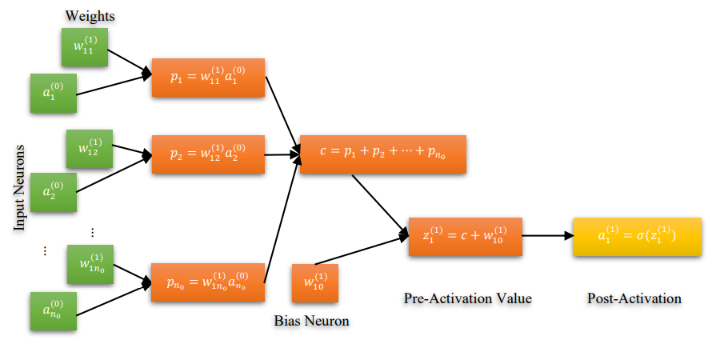
\includegraphics[width=\linewidth]{Images/04_Images/11.png}
    \caption{Đồ thị tính toán cho một nơ-ron}
\end{figure}
\paragraph{Ví dụ: biểu diễn một hàm bằng đồ thị tính toán\\}
Xét hàm hai biến
\begin{equation}
    F(x, y) = x^2 (x + y).
\end{equation}
Thay vì biểu diễn toàn bộ hàm bằng một biểu thức duy nhất, ta phân rã quá trình tính toán thành các phép toán trung gian. Đặt:
\begin{equation}
    c = x^2, \qquad s = x + y.
\end{equation}
Khi đó,
\begin{equation}
    F = cs.
\end{equation}
Đồ thị tính toán tương ứng có thể được mô tả bởi chuỗi phụ thuộc
\begin{equation}
    x, y \longrightarrow
    \begin{cases}
        c = x^2, \\
        s = x + y,
    \end{cases}
    \longrightarrow F = cs.
\end{equation}
Với $x = 2$ và $y = 3$, quá trình tính toán lần lượt cho
\begin{equation}
    c = 2^2 = 4, \qquad s = 2 + 3 = 5, \qquad F = 4 \cdot 5 = 20.
\end{equation}
Kết quả này tương đương với việc tính trực tiếp
\begin{equation}
    F = x^2 (x + y) = 2^2 (2 + 3) = 20.
\end{equation}
\begin{figure}[H]
    \centering
    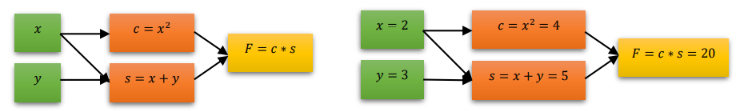
\includegraphics[width=\linewidth]{Images/04_Images/10.png}
    \caption{Đồ thị tính toán của hàm $F=x^2(x+y)$.}
\end{figure}
Ví dụ trên cho thấy đồ thị tính toán không thay đổi giá trị của hàm; thay vào đó, nó biểu diễn biểu thức dưới dạng một tập các phép tính cục bộ và các quan hệ phụ thuộc giữa chúng. Đây là đặc điểm có ý nghĩa quan trọng đối với việc tính đạo hàm bằng quy tắc chuỗi.

\subsubsection{Vi phân tự động}
Vi phân tự động là một phương pháp tính toán cho phép xác định đạo hàm của các hàm số được biểu diễn thông qua một chuỗi hữu hạn các phép toán số học cơ bản và các hàm sơ cấp. Phương pháp này có vai trò quan trọng trong tính toán khoa học, tối ưu hóa và học sâu, đặc biệt trong việc tính đạo hàm của hàm mất mát đối với các tham số của mạng nơ-ron.

Ý tưởng cơ bản của vi phân tự động dựa trên thực tế rằng một phép tính số học dù phức tạp đến đâu cũng có thể được phân rã thành một số hữu hạn các phép toán cơ bản, chẳng hạn như phép cộng, phép trừ, phép nhân, phép chia, cùng với các hàm sơ cấp như hàm mũ, hàm logarit và các hàm lượng giác. Đạo hàm của từng phép toán và hàm sơ cấp này có thể được xác định trực tiếp. Bằng cách kết hợp các đạo hàm tương ứng theo quy tắc chuỗi, ta có thể xác định đạo hàm của toàn bộ hàm mà không cần khai triển toàn bộ biểu thức giải tích.

Để làm rõ cơ chế tính đạo hàm, xét một hàm hợp đơn giản:
$y =g_3\!\left(g_2\!\left(g_1(x)\right)\right).$

Đặt:
$$v_0 = x, \quad v_1 = g_1(v_0), \quad v_2 = g_2(v_1), \quad v_3 = g_3(v_2) = y.$$


Ở đây, $v_0$ là đại lượng đầu vào, $v_1, v_2$ là các đại lượng trung gian và $v_3=y$ là đại lượng đầu ra. Các đại lượng này tạo thành một chuỗi phụ thuộc:
\[
v_0 \longrightarrow v_1 \longrightarrow v_2 \longrightarrow v_3.
\]

Theo quy tắc chuỗi, đạo hàm của $y$ theo $x$ được xác định bởi:
\begin{equation}
\frac{\partial y}{\partial x} = \frac{\partial y}{\partial v_2} \frac{\partial v_2}{\partial v_1} \frac{\partial v_1}{\partial x}.
\end{equation}

Do $v_3 = y$, ta có thể viết:
\begin{equation}
\frac{\partial y}{\partial x} = \frac{\partial v_3}{\partial v_2} \frac{\partial v_2}{\partial v_1} \frac{\partial v_1}{\partial v_0}.
\end{equation}
Công thức trên cho thấy đạo hàm của hàm hợp có thể được tính bằng cách kết hợp các đạo hàm cục bộ từ những đại lượng trung gian trong quá trình tính toán. Vi phân tự động khai thác chính cấu trúc này để tính đạo hàm mà không cần xây dựng và khai triển toàn bộ biểu thức đạo hàm.

Có hai phương thức cơ bản để thực hiện vi phân tự động: \emph{chế độ thuận} và \emph{chế độ đảo}.
\begin{itemize}
    \item \textbf{Chế độ thuận:} Quá trình tính đạo hàm được thực hiện theo cùng chiều với quá trình tính giá trị, tức từ các đại lượng đầu vào đến đại lượng đầu ra.
    \[v_0 \longrightarrow v_1 \longrightarrow \cdots
    \longrightarrow v_n,\]
    trong đó $v_0=x$ là biến độc lập và $v_n=y$ là đại lượng đầu ra. Ta lần lượt tính đạo hàm của từng đại lượng trung gian theo $x$. Theo quy tắc chuỗi, ta có quan hệ truy hồi:
    $$\frac{\partial v_i}{\partial x}
    =\frac{\partial v_i}{\partial v_{i-1}}
    \frac{\partial v_{i-1}}{\partial x},\qquad i=1,\ldots,n.$$
    Sau khi thực hiện tuần tự các phép tính trên (với $v_n=y$), ta thu được:
    $$\frac{\partial y}{\partial x}
    =\frac{\partial v_n}{\partial x}.$$
    Để biểu diễn ngắn gọn đạo hàm được tích lũy tại mỗi đại lượng trung gian, đặt
    \[\dot{v}_i=\frac{\partial v_i}{\partial x},\qquad i=0,\ldots,n.\]
    Khi đó, quan hệ truy hồi được viết dưới dạng
    \[\dot{v}_i=\frac{\partial v_i}{\partial v_{i-1}}
    \dot{v}_{i-1},\qquad i=1,\ldots,n,\]
    với điều kiện khởi đầu
    \[\dot{v}_0=\frac{\partial v_0}{\partial x}=1.\]
    Như vậy, chế độ thuận lần lượt truyền đạo hàm từ biến độc lập $x$ qua các đại lượng trung gian $v_1,\ldots,v_{n-1}$ đến đại lượng đầu ra $y=v_n$. Đại lượng $\dot{v}_i$ biểu diễn sự biến thiên của $v_i$ theo biến độc lập $x$ và được tính dựa trên đạo hàm cục bộ
    $\partial v_i/\partial v_{i-1}$.
    
    \item \textbf{Chế độ đảo:} Quá trình tính đạo hàm ngược chiều với quá trình tính giá trị, tức từ đại lượng đầu ra về các đại lượng đầu vào.
    \[v_0 \longrightarrow v_1 \longrightarrow \cdots\longrightarrow v_n = y,\]
    
    trong đó $v_0=x$ là biến đầu vào và $v_n=y$ là đại lượng đầu ra. Ta bắt đầu từ đại lượng đầu ra $y$ và lần lượt tính đạo hàm của $y$ theo các đại lượng trung gian theo chiều ngược lại. Theo quy tắc chuỗi, ta có quan hệ truy hồi:
    \begin{equation}
    \frac{\partial y}{\partial v_i}
    =\frac{\partial y}{\partial v_{i+1}}
    \frac{\partial v_{i+1}}{\partial v_i},\qquad i=n-1,\ldots,0.
    \end{equation}
    
    Do $v_0=x$, tại bước cuối cùng ta thu được
    \begin{equation}
    \frac{\partial y}{\partial x}=\frac{\partial y}{\partial v_0}.
    \end{equation}
    
    Để biểu diễn ngắn gọn đạo hàm được tích lũy tại mỗi đại lượng trung gian, đặt
    \begin{equation}
    \overline{v}_i=\frac{\partial y}{\partial  v_i},\qquad i=0,\ldots,n.
    \end{equation}
    Khi đó, quan hệ truy hồi của quá trình tích lũy ngược được viết dưới dạng
    \begin{equation}
    \overline{v}_i=\overline{v}_{i+1}\frac{\partial v_{i+1}}{\partial v_i},\qquad i=n-1,\ldots,0,
    \end{equation}
    với điều kiện khởi đầu
    \begin{equation}
    \overline{v}_n=\frac{\partial y}{\partial v_n}=1.
    \end{equation}
\end{itemize}
Như vậy, chế độ ngược bắt đầu từ đại lượng đầu ra và lần lượt truyền đạo hàm về các đại lượng trung gian rồi đến các biến đầu vào. Trong đồ thị tính toán tổng quát, giá trị đạo hàm tích lũy tại một biến trung gian được xác định bằng tổng các đóng góp truyền ngược từ các nút phụ thuộc trực tiếp vào biến đó. Do đó, các đạo hàm theo nhiều biến đầu vào có thể được tính thông qua cùng một quá trình truyền ngược trên đồ thị tính toán.

\paragraph{So sánh hai chế độ tích lũy đạo hàm}

Xét ánh xạ tổng quát:
\begin{equation}
f: \mathbb{R}^n \rightarrow \mathbb{R}^m,
\end{equation}
trong đó $n$ và $m$ lần lượt là số chiều của không gian đầu vào và không gian đầu ra. Ký hiệu:
\begin{equation}
\mathbf{x} = (x_1, \dots, x_n)^{\top} \in \mathbb{R}^n, \qquad \mathbf{y} = f(\mathbf{x}) = (y_1, \dots, y_m)^{\top} \in \mathbb{R}^m.
\end{equation}
Ma trận đạo hàm của $f$ tại $\mathbf{x}$ được gọi là ma trận Jacobi, ký hiệu:
\begin{equation}
\mathbf{J}_f(\mathbf{x}) = \left[ \frac{\partial y_i}{\partial x_j} \right]_{\substack{i=1,\dots,m \\ j=1,\dots,n}} \in \mathbb{R}^{m \times n}.
\end{equation}

\begin{itemize}
    \item \textbf{Chế độ thuận:} Khi $n \ll m$, chế độ thuận phù hợp hơn vì mỗi lần tích lũy xuôi có thể cố định một biến đầu vào và tính đạo hàm của toàn bộ các đại lượng đầu ra theo biến đó. Cụ thể, với biến đầu vào $x_j$, quá trình tích lũy xuôi cho phép xác định đồng thời:
    \begin{equation}
    \frac{\partial y_1}{\partial x_j}, \frac{\partial y_2}{\partial x_j}, \dots, \frac{\partial y_m}{\partial x_j}.
    \end{equation}
    Các đạo hàm này tạo thành cột thứ $j$ của ma trận Jacobi:
    \begin{equation}
    \mathbf{J}_f(\mathbf{x})_{:,j} = 
    \begin{bmatrix}
    \dfrac{\partial y_1}{\partial x_j} \\
    \vdots \\
    \dfrac{\partial y_m}{\partial x_j}
    \end{bmatrix}.
    \end{equation}
    Do đó, để xác định toàn bộ ma trận Jacobi bằng chế độ thuận, cần thực hiện quá trình tích lũy xuôi tương ứng với từng biến đầu vào. Số lần tích lũy (số bước duyệt qua đồ thị) cần thiết là $n$.

    \item \textbf{Chế độ đảo:} Khi $n \gg m$, chế độ đảo phù hợp hơn vì mỗi lần tích lũy ngược có thể cố định một đại lượng đầu ra và tính đạo hàm của đại lượng đó theo toàn bộ các biến đầu vào. Cụ thể, với đầu ra $y_i$, quá trình tích lũy ngược cho phép xác định đồng thời:
    \begin{equation}
    \frac{\partial y_i}{\partial x_1}, \frac{\partial y_i}{\partial x_2}, \dots, \frac{\partial y_i}{\partial x_n}.
    \end{equation}
    Các đạo hàm này tạo thành hàng thứ $i$ của ma trận Jacobi:
    \begin{equation}
    \mathbf{J}_f(\mathbf{x})_{i,:} = 
    \begin{bmatrix}
    \dfrac{\partial y_i}{\partial x_1} & \cdots & \dfrac{\partial y_i}{\partial x_n}
    \end{bmatrix}.
    \end{equation}
    Do đó, để xác định toàn bộ ma trận Jacobi bằng chế độ đảo, cần thực hiện quá trình tích lũy ngược tương ứng với từng biến đầu ra. Số lần tích lũy cần thiết là $m$.
\end{itemize}

Từ đó, khi $n \ll m$, chế độ thuận tốn ít chi phí tính toán hơn; ngược lại, khi $n \gg m$, chế độ đảo lại tối ưu hơn. Sự khác biệt về số lần tích lũy là một cơ sở quan trọng để lựa chọn chế độ vi phân tự động phù hợp với số chiều của không gian đầu vào và đầu ra.


\paragraph{Mối liên hệ với lan truyền ngược trong mạng nơ-ron\\}
Đối với mạng nơ-ron có L lớp, các tham số của mô hình có thể được xem là các biến của một ánh xạ từ không gian tham số đến giá trị của hàm mất mát. Ký hiệu tập các tham số của mạng là
\begin{equation}
\boldsymbol{\Theta}
=
\left\{
\mathbf{W}^{[l]},\mathbf{b}^{[l]}
\right\}_{l=1}^{L},
\end{equation}
trong đó $\mathbf{W}^{[l]}$ và $\mathbf{b}^{[l]}$ lần lượt là ma trận trọng số và vectơ độ chệch của lớp thứ $l$, $l=1,...L$. 

Giả sử tổng số tham số của mạng là $N$. Khi sắp xếp toàn bộ các phần tử của các ma trận trọng số và các véc-tơ độ chệch theo một thứ tự xác định thành một véc-tơ duy nhất, ta thu được véc-tơ tham số:
\begin{equation}
\boldsymbol{\theta} =
\begin{bmatrix}
\theta_1 & \theta_2 & \cdots & \theta_N
\end{bmatrix}^{\mathsf T}
\in\mathbb{R}^{N}.
\end{equation}
Trong đó:
\begin{itemize}
    \item $\boldsymbol{\theta}$: Véc-tơ tham số của mạng, được tạo thành bằng cách sắp xếp toàn bộ các tham số của mạng thành một véc-tơ duy nhất.
    \item $\theta_i$: Tham số thứ $i$ của mạng ($i=1,\ldots,N$), tương ứng với một phần tử của ma trận trọng số hoặc véc-tơ độ chệch thuộc một lớp cụ thể.
    \item $N$: Tổng số tham số của mạng.
    \item $\mathsf{T}$: Phép chuyển vị ma trận/véc-tơ, qua đó chuyển véc-tơ hàng $\begin{bmatrix} \theta_1 & \theta_2 & \cdots & \theta_N \end{bmatrix}$ thành véc-tơ cột.
    \item $\mathbb{R}^{N}$: Không gian véc-tơ thực $N$ chiều; do đó, ký hiệu $\boldsymbol{\theta}\in\mathbb{R}^{N}$ cho biết véc-tơ tham số có $N$ thành phần thực.
\end{itemize}
Với hàm mất mát vô hướng $\mathcal{L}=\mathcal{L}(\boldsymbol{\theta}),$ có thể được xem như một ánh xạ:
\begin{equation}
\mathcal{L}:\mathbb{R}^{N}\rightarrow\mathbb{R}.
\end{equation}

Trong biểu diễn này, không gian đầu vào của ánh xạ có $N$ chiều, tương ứng với tổng số tham số của mạng, trong khi không gian đầu ra chỉ có một chiều do hàm mất mát nhận giá trị vô hướng. Vì số lượng tham số của mạng thường rất lớn, ta có: $N\gg 1.$


Do đó, bài toán tính đạo hàm của hàm mất mát trong lan truyền ngược thuộc trường hợp ánh xạ có số chiều đầu vào lớn hơn rất nhiều so với số chiều đầu ra. Trong trường hợp này, vi phân tự động chế độ đảo phù hợp hơn. Chỉ với \textbf{một lần} lan truyền ngược duy nhất, ta có thể tính được đạo hàm của hàm mất mát theo toàn bộ các tham số:
\begin{equation}
\frac{\partial \mathcal{L}}{\partial \theta_1}, \frac{\partial \mathcal{L}}{\partial \theta_2}, \dots, \frac{\partial \mathcal{L}}{\partial \theta_N}.
\end{equation}
Các đạo hàm vô hướng này sau đó được tái định dạng lại tương ứng với kích thước của ma trận trọng số và véc-tơ độ chệch tại từng lớp để thu được:
\begin{equation}
\frac{\partial \mathcal{L}}{\partial \mathbf{W}^{[l]}} \quad \text{và} \quad \frac{\partial \mathcal{L}}{\partial \mathbf{b}^{[l]}}, \qquad l = 1, \dots, L.
\end{equation}
Cơ chế này chính là cơ sở toán học của lan truyền ngược trong mạng nơ-ron.

Như vậy, vi phân tự động cung cấp một phương pháp tổng quát để tính đạo hàm dựa trên cấu trúc của đồ thị tính toán. Chế độ thuận truyền sự phụ thuộc của đạo hàm từ đầu vào đến đầu ra và đặc biệt phù hợp khi số chiều đầu vào nhỏ hơn đáng kể số chiều đầu ra. Ngược lại, chế độ đảo truyền sự phụ thuộc của đạo hàm từ đầu ra về đầu vào và là phương pháp phù hợp khi số chiều đầu vào lớn hơn đáng kể số chiều đầu ra. Lan truyền ngược trong học sâu chính là trường hợp áp dụng của chế độ đảo cho bài toán tính gradient của một hàm mất mát vô hướng theo tham số của mạng nơ-ron.
\paragraph{Minh họa tính toán cho vi phân tự động chế độ thuận và chế độ đảo\\}
Xét hàm vô hướng hai biến:
\begin{equation}
    y = f(x_1,x_2) = \ln(x_1) + x_1 x_2 - \sin(x_2).
    \label{eq:ad_example_function}
\end{equation}
Mục tiêu là tính véc-tơ đạo hàm:
\begin{equation}
    \nabla f(x_1,x_2) = 
    \begin{bmatrix}
        \dfrac{\partial y}{\partial x_1} \\[6pt]
        \dfrac{\partial y}{\partial x_2}
    \end{bmatrix}
\end{equation}
bằng hai phương thức của vi phân tự động: chế độ thuận và chế độ đảo.

\paragraph{Xây dựng đồ thị tính toán:\\}

Để áp dụng vi phân tự động, hàm \eqref{eq:ad_example_function} được phân rã thành một chuỗi các phép toán cơ bản. Đặt:
\begin{equation}
\begin{aligned}
    v_{-1} &= x_1, \\
    v_0 &= x_2, \\
    v_1 &= \ln(v_{-1}), \\
    v_2 &= v_{-1} v_0, \\
    v_3 &= \sin(v_0), \\
    v_4 &= v_1 + v_2, \\
    v_5 &= v_4 - v_3 = y.
\end{aligned}
\label{eq:ad_example_graph}
\end{equation}

Các đạo hàm cục bộ tương ứng là:
\begin{equation}
    \frac{\partial v_1}{\partial v_{-1}} = \frac{1}{v_{-1}},
\end{equation}
\begin{equation}
    \frac{\partial v_2}{\partial v_{-1}} = v_0, \qquad \frac{\partial v_2}{\partial v_0} = v_{-1},
\end{equation}
\begin{equation}
    \frac{\partial v_3}{\partial v_0} = \cos(v_0),
\end{equation}
và
\begin{equation}
    \frac{\partial v_4}{\partial v_1} = \frac{\partial v_4}{\partial v_2} = \frac{\partial v_5}{\partial v_4} = 1, \qquad \frac{\partial v_5}{\partial v_3} = -1.
\end{equation}
Đồ thị tính toán của hàm có cấu trúc:
\begin{equation}
    (x_1,x_2) \longrightarrow (v_1,v_2,v_3) \longrightarrow v_4 \longrightarrow y.
\end{equation}
Việc phân rã này cho phép tính các đạo hàm của hàm đầu ra theo các biến đầu vào bằng cách sử dụng các đạo hàm cục bộ tại từng nút của đồ thị tính toán.
\paragraph{Tính đạo hàm bằng chế độ thuận:\\}
Trong chế độ thuận, đạo hàm được truyền từ các biến đầu vào đến biến đầu ra. Với một biến độc lập $x_j$, đặt giá trị tiếp tuyến tại đỉnh $v_i$ là:
\begin{equation}
    \dot{v}_i = \frac{\partial v_i}{\partial x_j}.
\end{equation}
Các giá trị này được tính tuần tự theo chiều thuận của đồ thị.
\begin{itemize}
    \item \textit{Đạo hàm theo $x_1$:}
    Chọn $x_1$ làm biến độc lập. Khi đó:
    \begin{equation}
        \dot{v}_{-1} = \frac{\partial v_{-1}}{\partial x_1} = 1, \qquad \dot{v}_0 = \frac{\partial v_0}{\partial x_1} = 0.
    \end{equation}
    Tại đỉnh $v_1 = \ln(v_{-1})$:
    \begin{equation}
        \dot{v}_1 = \frac{\partial v_1}{\partial v_{-1}}\dot{v}_{-1} = \frac{1}{v_{-1}} = \frac{1}{x_1}.
    \end{equation}
    Tại đỉnh $v_2 = v_{-1} v_0$, áp dụng quy tắc đạo hàm của tích:
    \begin{equation}
    \begin{aligned}
        \dot{v}_2 &= \frac{\partial v_2}{\partial v_{-1}}\dot{v}_{-1} + \frac{\partial v_2}{\partial v_0}\dot{v}_0 \\
        &= v_0(1) + v_{-1}(0) = x_2.
    \end{aligned}
    \end{equation}
    Tại đỉnh $v_3 = \sin(v_0)$:
    \begin{equation}
        \dot{v}_3 = \frac{\partial v_3}{\partial v_0}\dot{v}_0 = \cos(v_0)(0) = 0.
    \end{equation} 
    Tiếp theo:
    \begin{equation}
        \dot{v}_4 = \dot{v}_1 + \dot{v}_2 = \frac{1}{x_1} + x_2.
    \end{equation}
    Cuối cùng, vì $v_5 = v_4 - v_3$:
    \begin{equation}
        \dot{v}_5 = \dot{v}_4 - \dot{v}_3 = \frac{1}{x_1} + x_2.
    \end{equation}
    Do $v_5 = y$, suy ra:
    \begin{equation}
        \frac{\partial y}{\partial x_1} = \frac{1}{x_1} + x_2.
        \label{eq:forward_dx1}
    \end{equation}

    \item \textit{Đạo hàm theo $x_2$:}
    Tiếp tục thực hiện một lượt tích lũy thuận với $x_2$ làm biến độc lập. Khi đó:
    \begin{equation}
        \dot{v}_{-1} = \frac{\partial v_{-1}}{\partial x_2} = 0, \qquad \dot{v}_0 = \frac{\partial v_0}{\partial x_2} = 1.
    \end{equation}
    Tại đỉnh $v_1 = \ln(v_{-1})$:
    \begin{equation}
        \dot{v}_1 = \frac{1}{v_{-1}}\dot{v}_{-1} = 0.
    \end{equation}
    Tại đỉnh $v_2 = v_{-1} v_0$:
    \begin{equation}
    \begin{aligned}
        \dot{v}_2 &= v_0\dot{v}_{-1} + v_{-1}\dot{v}_0 \\
        &= x_2(0) + x_1(1) = x_1.
    \end{aligned}
    \end{equation}
    Tại đỉnh $v_3 = \sin(v_0)$:
    \begin{equation}
        \dot{v}_3 = \cos(v_0)\dot{v}_0 = \cos(x_2).
    \end{equation}
    Tại đỉnh $v_4$:
    \begin{equation}
        \dot{v}_4 = \dot{v}_1 + \dot{v}_2 = x_1,
    \end{equation}
    và $v_5$
    \begin{equation}
        \dot{v}_5 = \dot{v}_4 - \dot{v}_3 = x_1 - \cos(x_2).
    \end{equation}
    Suy ra:
    \begin{equation}
        \frac{\partial y}{\partial x_2} = x_1 - \cos(x_2).
        \label{eq:forward_dx2}
    \end{equation}
    Từ \eqref{eq:forward_dx1} và \eqref{eq:forward_dx2}, véc-tơ đạo hàm thu được bằng chế độ thuận là:
    \begin{equation}
        \nabla f(x_1,x_2) = 
        \begin{bmatrix}
            \dfrac{1}{x_1} + x_2 \\[6pt]
            x_1 - \cos(x_2)
        \end{bmatrix}.
        \label{eq:forward_gradient}
    \end{equation}
    Có thể nhận thấy rằng để thu được toàn bộ véc-tơ đạo hàm của hàm $f:\mathbb{R}^2 \rightarrow \mathbb{R}$ bằng chế độ thuận, cần thực hiện hai lượt tích lũy, tương ứng với hai hướng độc lập $x_1$ và $x_2$.
\end{itemize}
Chi tiết quá trình tính toán theo chiều thuận và tích lũy giá trị các biến trung gian tại điểm $(x_1,x_2) = (2,5)$, với giá trị khởi tạo là $\dot{x}_1 = \dot{v}_{-1} = 1$ và $\dot{x}_2 = \dot{v}_0 = 0$.
\begin{table}[H]
\centering
\renewcommand{\arraystretch}{1.35}
\begin{tabular*}{\textwidth}{@{\extracolsep{\fill}} l l | l l @{}}
\hline
\multicolumn{2}{l|}{Chuỗi giá trị các biến tính toán} & \multicolumn{2}{l}{Chuỗi giá trị các biến trung gian} \\
\hline
$v_{-1} = x_1$        & $= 2$             & $\dot{v}_{-1} = \dot{x}_1$                             & $= 1$ \\
$v_0 = x_2$           & $= 5$             & $\dot{v}_0 = \dot{x}_2$                                & $= 0$ \\
$v_1 = \ln(v_{-1})$   & $\approx 0.693$   & $\dot{v}_1 = \dot{v}_{-1} / v_{-1}$                    & $= 1 / 2 = 0.5$ \\
$v_2 = v_{-1} \times v_0$& $= 2 \times 5 = 10$& $\dot{v}_2 = \dot{v}_{-1} \times v_0 + v_{-1} \times \dot{v}_0$ & $= 1 \times 5 + 2 \times 0 = 5$ \\
$v_3 = \sin(v_0)$     & $\approx -0.959$  & $\dot{v}_3 = \dot{v}_0 \cos(v_0)$                      & $= 0 \times \cos(5) = 0$ \\
$v_4 = v_1 + v_2$     & $= 0.693 + 10 = 10.693$& $\dot{v}_4 = \dot{v}_1 + \dot{v}_2$                 & $= 0.5 + 5 = 5.5$ \\
$v_5 = v_4 - v_3$     & $= 10.693 - (-0.959)$& $\dot{v}_5 = \dot{v}_4 - \dot{v}_3$                  & $= 5.5 - 0 = 5.5$ \\
$y = v_5$             & $= 11.652$        & $\dot{y} = \dot{v}_5$                                  & $= 5.5$ \\
\hline
\end{tabular*}
\caption{Ví dụ minh họa vi phân tự động ở chế độ thuận tính đạo hàm riêng $\frac{\partial y}{\partial x_1}$, đối với hàm $y = f(x_1,x_2) = \ln(x_1) + x_1 x_2 - \sin(x_2)$ tại điểm $(x_1,x_2) = (2,5)$.}
\end{table}

\begin{table}[H]
\centering
\renewcommand{\arraystretch}{1.35}
\begin{tabular*}{\textwidth}{@{\extracolsep{\fill}} l l | l l @{}}
\hline
\multicolumn{2}{l|}{Chuỗi giá trị các biến tính toán} & \multicolumn{2}{l}{Chuỗi giá trị các biến trung gian} \\
\hline
$v_{-1} = x_1$        & $= 2$             & $\dot{v}_{-1} = \dot{x}_1$                             & $= 0$ \\
$v_0 = x_2$           & $= 5$             & $\dot{v}_0 = \dot{x}_2$                                & $= 1$ \\
$v_1 = \ln(v_{-1})$   & $\approx 0.693$   & $\dot{v}_1 = \dot{v}_{-1} / v_{-1}$                    & $= 0 / 2 = 0$ \\
$v_2 = v_{-1} \times v_0$& $= 2 \times 5 = 10$& $\dot{v}_2 = \dot{v}_{-1} \times v_0 + v_{-1} \times \dot{v}_0$ & $= 0 \times 5 + 2 \times 1 = 2$ \\
$v_3 = \sin(v_0)$     & $\approx -0.959$  & $\dot{v}_3 = \dot{v}_0 \cos(v_0)$                      & $= 1 \times \cos(5) \approx 0.284$ \\
$v_4 = v_1 + v_2$     & $= 0.693 + 10 = 10.693$& $\dot{v}_4 = \dot{v}_1 + \dot{v}_2$                 & $= 0 + 2 = 2$ \\
$v_5 = v_4 - v_3$     & $= 10.693 - (-0.959)$& $\dot{v}_5 = \dot{v}_4 - \dot{v}_3$                  & $= 2 - 0.284 = 1.716$ \\
$y = v_5$             & $= 11.652$        & $\dot{y} = \dot{v}_5$                                  & $= 1.716$ \\
\hline
\end{tabular*}
\caption{Ví dụ minh họa vi phân tự động ở chế độ thuận nhằm tính đạo hàm riêng $\frac{\partial y}{\partial x_2}$ đối với hàm $y = f(x_1,x_2) = \ln(x_1) + x_1 x_2 - \sin(x_2)$ tại điểm $(x_1,x_2) = (2,5)$.}
\end{table}

\begin{figure}[H]
    \centering
    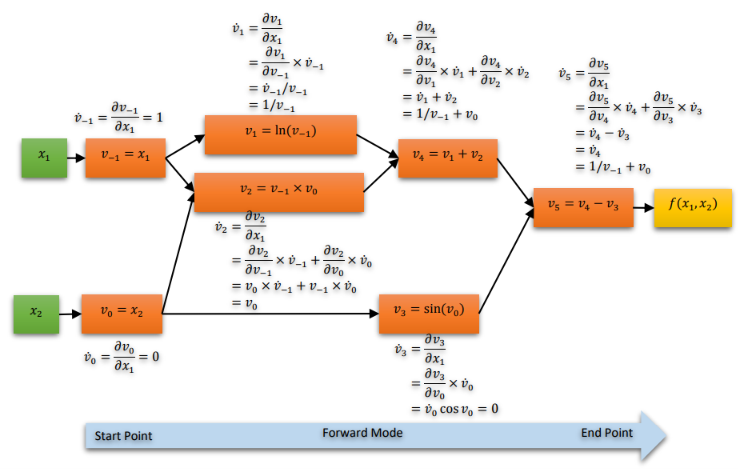
\includegraphics[width=\linewidth]{Images/04_Images/13.png}
    \caption{Ví dụ minh họa chế độ thuận trên đồ thị tính toán của hàm $y = \ln(x_1) + x_1 x_2 - \sin(x_2)$.}
    \label{4.13}
\end{figure}

\paragraph{Tính đạo hàm bằng chế độ đảo\\}

Trong chế độ đảo, quá trình tích lũy đạo hàm được thực hiện theo chiều từ đầu ra về các biến đầu vào. Đặt giá trị liên hợp tại đỉnh $v_i$ là:
\begin{equation}
    \bar{v}_i = \frac{\partial y}{\partial v_i}.
\end{equation}

Trước tiên, giá trị liên hợp tại đỉnh đầu ra được khởi tạo, do $v_5 = y$:
\begin{equation}
    \bar{v}_5 = \frac{\partial y}{\partial v_5} = 1.
\end{equation}

Từ $v_5 = v_4 - v_3$, ta có:
\begin{equation}
    \bar{v}_4 = \bar{v}_5 \frac{\partial v_5}{\partial v_4} = 1(1) = 1,
\end{equation}
và
\begin{equation}
    \bar{v}_3 = \bar{v}_5 \frac{\partial v_5}{\partial v_3} = 1(-1) = -1.
\end{equation}

Tiếp theo, từ $v_4 = v_1 + v_2$:
\begin{equation}
    \bar{v}_1 = \bar{v}_4 \frac{\partial v_4}{\partial v_1} = 1(1) = 1,
\end{equation}
\begin{equation}
    \bar{v}_2 = \bar{v}_4 \frac{\partial v_4}{\partial v_2} = 1(1) = 1.
\end{equation}

Xét nhánh $v_1 = \ln(v_{-1})$:
\begin{equation}
    \bar{v}_{-1}^{(1)} = \bar{v}_1 \frac{\partial v_1}{\partial v_{-1}} = 1\left(\frac{1}{v_{-1}}\right) = \frac{1}{x_1}.
\end{equation}

Xét nhánh $v_2 = v_{-1} v_0$:
\begin{equation}
    \bar{v}_{-1}^{(2)} = \bar{v}_2 \frac{\partial v_2}{\partial v_{-1}} = 1(v_0) = x_2,
\end{equation}
và
\begin{equation}
    \bar{v}_0^{(2)} = \bar{v}_2 \frac{\partial v_2}{\partial v_0} = 1(v_{-1}) = x_1.
\end{equation}

Cuối cùng, xét nhánh $v_3 = \sin(v_0)$:
\begin{equation}
    \bar{v}_0^{(3)} = \bar{v}_3 \frac{\partial v_3}{\partial v_0} = -1(\cos(v_0)) = -\cos(x_2).
\end{equation}

Do $v_{-1} = x_1$ và $v_0 = x_2$, các đóng góp tại mỗi biến đầu vào được cộng dồn lại. Đối với $x_1$:
\begin{equation}
\begin{aligned}
    \frac{\partial y}{\partial x_1} &= \bar{v}_{-1} = \bar{v}_{-1}^{(1)} + \bar{v}_{-1}^{(2)} \\
    &= \frac{1}{x_1} + x_2.
\end{aligned}
\end{equation}

Đối với $x_2$:
\begin{equation}
\begin{aligned}
    \frac{\partial y}{\partial x_2} &= \bar{v}_0 = \bar{v}_0^{(2)} + \bar{v}_0^{(3)} \\
    &= x_1 - \cos(x_2).
\end{aligned}
\end{equation}

Do đó, chế độ đảo cũng thu được kết quả đồng nhất:
\begin{equation}
    \nabla f(x_1,x_2) = 
    \begin{bmatrix}
        \dfrac{1}{x_1} + x_2 \\[6pt]
        x_1 - \cos(x_2)
    \end{bmatrix}.
    \label{eq:reverse_gradient}
\end{equation}

Chi tiết quá trình tính toán các giá trị và tích lũy các giá trị các biến liên hợp theo chiều đảo tại điểm $(x_1,x_2) = (2,5)$ nhằm xác định các đạo hàm riêng của hàm đầu ra $y$ đối với các biến đầu vào $x_1$ và $x_2$.

\begin{table}[H]
\centering
\renewcommand{\arraystretch}{1.35} 
\begin{tabular*}{\textwidth}{@{\extracolsep{\fill}} l l | l l @{}}
\hline
\multicolumn{2}{l|}{Chuỗi giá trị các biến tính toán} & \multicolumn{2}{l}{Chuỗi giá trị các biến trung gian} \\
\hline
$v_{-1} = x_1$        & $= 2$             & $\bar{v}_5 = \bar{y}$                                                               & $= 1$ \\
$v_0 = x_2$           & $= 5$             & $\bar{v}_4 = \bar{v}_5 \frac{\partial v_5}{\partial v_4}$                           & $= 1 \times 1 = 1$ \\
$v_1 = \ln(v_{-1})$   & $\approx 0.693$   & $\bar{v}_3 = \bar{v}_5 \frac{\partial v_5}{\partial v_3}$                           & $= 1 \times (-1) = -1$ \\
$v_2 = v_{-1} \times v_0$& $= 10$         & $\bar{v}_2 = \bar{v}_4 \frac{\partial v_4}{\partial v_2}$                           & $= 1 \times 1 = 1$ \\
$v_3 = \sin(v_0)$     & $\approx -0.959$  & $\bar{v}_1 = \bar{v}_4 \frac{\partial v_4}{\partial v_1}$                           & $= 1 \times 1 = 1$ \\
$v_4 = v_1 + v_2$     & $\approx 10.693$  & $\bar{v}_0 = \bar{v}_2 \frac{\partial v_2}{\partial v_0} + \bar{v}_3 \frac{\partial v_3}{\partial v_0}$ & $= 1(2) + (-1)\cos(5) \approx 1.716$ \\
$v_5 = v_4 - v_3$     & $\approx 11.652$  & $\bar{v}_{-1} = \bar{v}_1 \frac{\partial v_1}{\partial v_{-1}} + \bar{v}_2 \frac{\partial v_2}{\partial v_{-1}}$ & $= 1(0.5) + 1(5) = 5.5$ \\
$y = v_5$             & $\approx 11.652$  & $\bar{\mathbf{x}} = (\bar{v}_{-1}, \bar{v}_0)$                                      & $= (5.5, \; 1.716)$ \\
\hline
\end{tabular*}
\caption{Ví dụ minh họa vi phân tự động ở chế độ đảo đối với hàm $y = f(x_1,x_2) = \ln(x_1) + x_1 x_2 - \sin(x_2)$ tại điểm $(x_1,x_2) = (2,5)$.}
\end{table}

\begin{figure}[H]
    \centering
    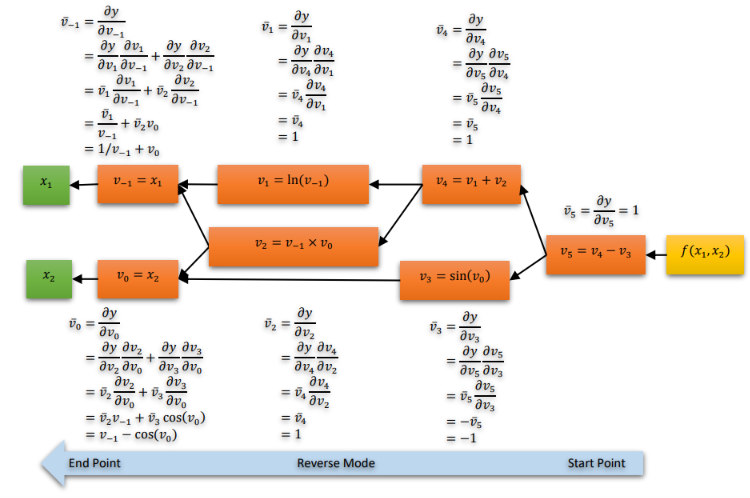
\includegraphics[width=\linewidth]{Images/04_Images/14.png}
    \caption{Ví dụ về chế độ đảo vi phân tự động trên đồ thị tính toán của hàm $y = \ln(x_1) + x_1 x_2 - \sin(x_2)$.}
    \label{4.14}
\end{figure}

\begin{lstlisting}[caption=Cài đặt chế độ thuận bằng thư viện NumPy]
import numpy as np

# --- (x_1,x_2) = (2,5) ---
x1, x2 = 2.0, 5.0

# --- Forward ---
# --- y = f(x_1,x_2) = ln(x_1) + x_1 x_2 - sin(x_2) ---
v1 = np.log(x1)
v2 = x1 * x2
v3 = np.sin(x2)
v4 = v1 + v2
y  = v4 - v3

# --- Forward mode x1 ---
dv1 = 1 / x1
dv2 = x2
dv3 = 0
dv4 = dv1 + dv2
dy_dx1 = dv4 - dv3

# --- Forward mode x2 ---
dv1 = 0
dv2 = x1
dv3 = np.cos(x2)
dv4 = dv1 + dv2
dy_dx2 = dv4 - dv3

# --- In cac gia tri ---
print(y)
print(dy_dx1, dy_dx2)
\end{lstlisting}

\begin{lstlisting}[caption=Cài đặt chế độ đảo bằng thư viện NumPy]
import numpy as np

# --- (x_1,x_2) = (2,5) ---
x1, x2 = 2.0, 5.0


# --- Reverse pass ---
# --- y = f(x_1,x_2) = ln(x_1) + x_1 x_2 - sin(x_2) ---
bar_v5 = 1.0

bar_v4 = bar_v5
bar_v3 = -bar_v5

bar_v1 = bar_v4
bar_v2 = bar_v4

bar_v_minus1 = bar_v1 * (1 / x1) + bar_v2 * x2
bar_v0 = bar_v2 * x1 + bar_v3 * np.cos(x2)

# --- In cac gia tri ---
print(bar_v_minus1, bar_v0)
\end{lstlisting}

\begin{lstlisting}[caption= Cơ chế vi phân tự động bằng PyTorch]
import torch

# --- (x_1,x_2) = (2,5) ---
x = torch.tensor([2.0, 5.0], requires_grad=True)

# --- y = f(x_1,x_2) = ln(x_1) + x_1 x_2 - sin(x_2) ---
y = torch.log(x[0]) + x[0] * x[1] - torch.sin(x[1])

y.backward()

# --- In cac gia tri ---
print(y.item())
print(x.grad)
\end{lstlisting}
\subsection{Bốn phương trình nền tảng của thuật toán lan truyền ngược}
Xét một mạng nơ-ron truyền thẳng gồm $L$ lớp. Với mỗi lớp $l \in \{1,2,\dots,L\}$, quá trình lan truyền tiến được xác định bởi:
\begin{equation}
\begin{aligned}
\mathbf a^{[0]}&=\mathbf x,\\
\mathbf z^{[l]}&=\mathbf W^{[l]}\mathbf a^{[l-1]}+\mathbf b^{[l]},
&\mathbf a^{[l]}&=\sigma^{[l]}(\mathbf z^{[l]}),\quad l=1,\ldots,L,\\
\widehat{\mathbf y}&=\mathbf a^{[L]}.
% &\mathcal L&=\ell(\mathbf a^{[L]},\mathbf y).
\end{aligned}
\label{eq:bp_forward}
\end{equation}
% Trong đó:
% \begin{itemize}
%     \item \(L\in\mathbb N\) là tổng số lớp của mạng, không tính lớp đầu vào; \(l\in\{1,\ldots,L\}\) là chỉ số của một lớp.
%     \item $n_l \in \mathbb{N}$: Số lượng nơ-ron tương ứng tại lớp $l$ (với $l = 0, 1, \dots, L$).
%     \item $\mathbf{a}^{[0]}, \mathbf{x} \in \mathbb{R}^{n_0}$: Véc-tơ đặc trưng đầu vào.
%     \item $\widehat{\mathbf{y}} \in \mathbb{R}^{n_L}$: Véc-tơ dự đoán đầu ra của mạng.
%     \item $\mathbf{W}^{[l]} \in \mathbb{R}^{n_l \times n_{l-1}}$: Ma trận trọng số kết nối từ lớp $l-1$ đến lớp $l$.
%     \item $\mathbf{b}^{[l]} \in \mathbb{R}^{n_l}$: Véc-tơ độ lệch tại lớp $l$.
%     \item $\mathbf{z}^{[l]} \in \mathbb{R}^{n_l}$: Véc-tơ giá trị tiền kích hoạt tại lớp $l$,
%     theo dạng thành phần, với $j \in \{1,\dots,n_l\}$:
%     \begin{equation}
%     z_j^{[l]} = \sum_{k=1}^{n^{[l-1]}} w_{jk}^{[l]}a_k^{[l-1]} + b_j^{[l]}, \qquad a_j^{[l]} = \sigma^{[l]}\!\left(z_j^{[l]}\right),
%     \end{equation}
%    trong đó $w_{jk}^{[l]}$ là trọng số liên kết nơ-ron thứ $k$ của lớp $l-1$ với nơ-ron thứ $j$ của lớp $l$, còn $b_j^{[l]}$ là độ lệch của nơ-ron thứ $j$ tại lớp $l$.
%     \item $\mathbf{a}^{[l]} \in \mathbb{R}^{n^{[l]}}$: Véc-tơ kích hoạt đầu ra tại lớp $l$.
%     \item $\sigma^{[l]}(\cdot)$: Hàm kích hoạt tác động theo từng phần tử tại lớp $l$.
% \end{itemize}
Hàm mất mát đối với một mẫu dữ liệu được ký hiệu bởi:
\begin{equation}
\mathcal{L} 
= \mathcal{L}\!\left(\mathbf{a}^{[L]},\mathbf{y}\right)
= \mathcal{L}\!\left(\hat{\mathbf{y}},\mathbf{y}\right)
\end{equation}
trong đó $\mathbf{y} \in \mathbb{R}^{n_L}$ là véc-tơ nhãn chuẩn. Mục tiêu của thuật toán lan truyền ngược là tính các đạo hàm của hàm mất mát đối với các tham số của từng lớp:
\begin{equation}
\frac{\partial\mathcal{L}}{\partial\mathbf{W}^{[l]}}, \qquad \frac{\partial\mathcal{L}}{\partial\mathbf{b}^{[l]}}, \qquad l=1,\dots,L.
\end{equation}
Ta định nghĩa \textbf{véc-tơ sai số tại lớp $l$, $l=0,...,L$}:
\begin{equation}
    \boldsymbol{\delta}^{[l]} \triangleq \nabla_{\mathbf{z}^{[l]}}\mathcal{L} = 
    \begin{bmatrix}
    \dfrac{\partial\mathcal{L}}{\partial z_1^{[l]}} \\[6pt]
    \dfrac{\partial\mathcal{L}}{\partial z_2^{[l]}} \\
    \vdots \\
    \dfrac{\partial\mathcal{L}}{\partial z_{n_l}^{[l]}}
    \end{bmatrix}
    \in \mathbb{R}^{n_l}.
\end{equation}
Trong đó:
\begin{itemize}
    \item $\boldsymbol{\delta}^{[l]} \in \mathbb{R}^{n_l}$: Véc-tơ sai số lan truyền ngược tại lớp $l$, bao gồm các đạo hàm riêng của hàm mất mát $\mathcal{L}$ đối với từng thành phần của véc-tơ tiền kích hoạt $\mathbf{z}^{[l]}$.
    \item $\nabla_{\mathbf{z}^{[l]}}\mathcal{L} \in \mathbb{R}^{n_l}$: Véc-tơ gradient của hàm mất mát $\mathcal{L}$ theo véc-tơ $\mathbf{z}^{[l]}$ (quy ước dạng véc-tơ cột).
    % \item $\triangleq$: Ký hiệu \textit{được định nghĩa là}, chỉ ra rằng biểu thức ở bên trái được định nghĩa là biểu thức ở bên phải.
\end{itemize}
Từ định nghĩa trên và áp dụng quy tắc chuỗi đối với hàm nhiều biến, ta thiết lập bốn hệ thức cơ bản của thuật toán lan truyền ngược.
\subsubsection{Phương trình thứ nhất: Sai số lan truyền ngược tại lớp đầu ra}
Mục tiêu của lan truyền ngược tại lớp đầu ra là tính gradient của hàm mất mát vô hướng $\mathcal{L}: \mathbb{R}^{n_L} \to \mathbb{R}$ đối với từng thành phần của véc-tơ tiền kích hoạt $\mathbf{z}^{[L]} = [z_1^{[L]}, \dots, z_{n_L}^{[L]}]^\top \in \mathbb{R}^{n_L}$. Ta định nghĩa véc-tơ sai số $\boldsymbol{\delta}^{[L]} \in \mathbb{R}^{n_L}$ với thành phần thứ $j$ là:
\begin{equation}
\delta_j^{[L]} \triangleq \frac{\partial \mathcal{L}}{\partial z_j^{[L]}}, \qquad j = 1, \dots, n_L.
\label{eq:delta_def}
\end{equation}
Do hàm mất mát $\mathcal{L}$ phụ thuộc vào $\mathbf{z}^{[L]}$ gián tiếp thông qua toàn bộ $n_L$ thành phần của véc-tơ kích hoạt đầu ra $\mathbf{a}^{[L]} = [a_1^{[L]}, \dots, a_{n_L}^{[L]}]^\top \in \mathbb{R}^{n_L}$, áp dụng quy tắc chuỗi đa biến:
\begin{equation}
\delta_j^{[L]} = \frac{\partial\mathcal{L}}{\partial z_j^{[L]}} = \sum_{k=1}^{n_L} \frac{\partial\mathcal{L}}{\partial a_k^{[L]}} \frac{\partial a_k^{[L]}}{\partial z_j^{[L]}}.
\label{eq:delta_chain}
\end{equation}
Vì hàm kích hoạt $\sigma^{[L]}: \mathbb{R} \to \mathbb{R}$ tác động độc lập trên từng thành phần, tức $a_k^{[L]} = \sigma^{[L]}\!\left(z_k^{[L]}\right)$. Khi lấy đạo hàm riêng của $a_k^{[L]}$ theo $z_j^{[L]}$, ta xét hai trường hợp:
\begin{itemize}
    \item Khi $k = j$: biến $a_j^{[L]}$ phụ thuộc trực tiếp vào $z_j^{[L]}$, do đó đạo hàm riêng chính là đạo hàm thông thường:
    \begin{equation}
    \frac{\partial a_j^{[L]}}{\partial z_j^{[L]}} = {\sigma^{[L]}}'\!\left(z_j^{[L]}\right).
    \end{equation}
    \item Khi $k \neq j$: biến $a_k^{[L]}$ hoàn toàn độc lập với $z_j^{[L]}$, do đó:
    \begin{equation}
    \frac{\partial a_k^{[L]}}{\partial z_j^{[L]}} = 0.
    \end{equation}
\end{itemize}
Biểu diễn gọn lại hai trường hợp trên thông qua ký hiệu Kronecker delta $\delta_{kj}$ ($\delta_{kj} = 1$ khi $k = j$ và $\delta_{kj} = 0$ khi $k \neq j$):
\begin{equation}
\frac{\partial a_k^{[L]}}{\partial z_j^{[L]}} = {\sigma^{[L]}}'\!\left(z_k^{[L]}\right) \delta_{kj}.
\label{eq:derivative_elementwise}
\end{equation}
Thay \eqref{eq:derivative_elementwise} vào biểu thức quy tắc chuỗi \eqref{eq:delta_chain}, ta thu được:
\begin{equation}
\begin{aligned}
    \delta_j^{[L]} &= \sum_{k=1}^{n_L} \frac{\partial\mathcal{L}}{\partial a_k^{[L]}} {\sigma^{[L]}}'\!\left(z_k^{[L]}\right) \delta_{kj} \\[6pt]
    &= \frac{\partial\mathcal{L}}{\partial a_j^{[L]}} {\sigma^{[L]}}'\!\left(z_j^{[L]}\right), \qquad \forall j = 1, \dots, n_L.
\end{aligned}
\label{eq:bp_scalar}
\end{equation}
Để chuyển hệ $n_L$ phương trình vô hướng ở \eqref{eq:bp_scalar} sang dạng ma trận-véc-tơ, ta sử dụng các định nghĩa toán học sau:
\begin{enumerate}
    \item \textbf{Véc-tơ gradient:} Theo quy ước véc-tơ cột, gradient của hàm mất mát vô hướng $\mathcal{L}$ đối với véc-tơ $\mathbf{a}^{[L]} \in \mathbb{R}^{n_L}$ là ánh xạ $\nabla_{\mathbf{a}^{[L]}}\mathcal{L}: \mathbb{R}^{n_L} \to \mathbb{R}^{n_L}$, được định nghĩa là véc-tơ chứa các đạo hàm riêng:
    \begin{equation}
    \nabla_{\mathbf{a}^{[L]}}\mathcal{L} \triangleq 
    \left[ \frac{\partial\mathcal{L}}{\partial a_1^{[L]}}, \frac{\partial\mathcal{L}}{\partial a_2^{[L]}}, \dots, \frac{\partial\mathcal{L}}{\partial a_{n_L}^{[L]}} \right]^\top =
    \begin{bmatrix} 
    \dfrac{\partial\mathcal{L}}{\partial a_1^{[L]}} \\[6pt] 
    \vdots \\ 
    \dfrac{\partial\mathcal{L}}{\partial a_{n_L}^{[L]}} 
    \end{bmatrix} \in \mathbb{R}^{n_L}.
    \end{equation}
    \item \textbf{Đạo hàm hàm kích hoạt theo từng phần tử:} Với hàm kích hoạt khả vi $\sigma^{[L]}: \mathbb{R} \to \mathbb{R}$ tác động theo từng phần tử lên $\mathbf{z}^{[L]}$, véc-tơ đạo hàm ${\sigma^{[L]}}'\!\left(\mathbf{z}^{[L]}\right) \in \mathbb{R}^{n_L}$ được định nghĩa bởi:
    \begin{equation}
    {\sigma^{[L]}}'\!\left(\mathbf{z}^{[L]}\right) \triangleq 
    \left[ {\sigma^{[L]}}'\!\left(z_1^{[L]}\right), {\sigma^{[L]}}'\!\left(z_2^{[L]}\right), \dots, {\sigma^{[L]}}'\!\left(z_{n_L}^{[L]}\right) \right]^\top =
    \begin{bmatrix} 
    {\sigma^{[L]}}'\!\left(z_1^{[L]}\right) \\[6pt] 
    \vdots \\ 
    {\sigma^{[L]}}'\!\left(z_{n_L}^{[L]}\right) 
    \end{bmatrix} \in \mathbb{R}^{n_L}.
    \end{equation}
    Trong đó $\triangleq$: Ký hiệu định nghĩa toán học (vế trái được định nghĩa bằng vế phải).
    \item \textbf{Tích Hadamard:} Cho hai véc-tơ tùy ý $\mathbf{u}, \mathbf{v} \in \mathbb{R}^n$, phép nhân từng thành phần là ánh xạ song tuyến tính $\odot: \mathbb{R}^n \times \mathbb{R}^n \to \mathbb{R}^n$, được định nghĩa hình thức bởi:
    \begin{equation}
    \mathbf{u} \odot \mathbf{v} \triangleq 
    \begin{bmatrix} 
    u_1 v_1 \\ 
    u_2 v_2 \\ 
    \vdots \\ 
    u_n v_n 
    \end{bmatrix} \in \mathbb{R}^n, \quad \text{tức } [\mathbf{u} \odot \mathbf{v}]_j = u_j v_j, \quad \forall j = 1, \dots, n.
    \end{equation}
    Trong đó $\triangleq$: Ký hiệu định nghĩa toán học (vế trái được định nghĩa bằng vế phải).
\end{enumerate}
Từ đây, ta thấy rằng thành phần thứ $j$ của véc-tơ sai số tại lớp đầu ra $\boldsymbol{\delta}^{[L]}$ chính là tích số của thành phần thứ $j$ thuộc $\nabla_{\mathbf{a}^{[L]}}\mathcal{L}$ với thành phần thứ $j$ thuộc ${\sigma^{[L]}}'\!\left(\mathbf{z}^{[L]}\right)$:
\begin{equation}
\delta_j^{[L]} = \left[ \nabla_{\mathbf{a}^{[L]}}\mathcal{L} \right]_j \cdot \left[ {\sigma^{[L]}}'\!\left(\mathbf{z}^{[L]}\right) \right]_j, \qquad \forall j = 1, \dots, n_L.
\end{equation}
Áp dụng định nghĩa của phép tích Hadamard, ta thu được phương trình cơ bản thứ nhất của thuật toán lan truyền ngược dưới dạng véc-tơ:
\begin{equation}
\boxed{
\boldsymbol{\delta}^{[L]} = \nabla_{\mathbf{a}^{[L]}}\mathcal{L} \odot {\sigma^{[L]}}'\!\left(\mathbf{z}^{[L]}\right)}
\label{eq:bp_vector}
\end{equation}
\subsubsection{Phương trình thứ hai: Lan truyền sai số về các lớp ẩn trước}
Mục tiêu của phương trình thứ hai là biểu diễn véc-tơ sai số ở các lớp ẩn $l$, ký hiệu: $\boldsymbol{\delta}^{[l]} \in \mathbb{R}^{n_l}$ thông qua véc-tơ sai số của lớp kế tiếp $\boldsymbol{\delta}^{[l+1]} \in \mathbb{R}^{n_{l+1}}$.
\paragraph{1. Khai triển quy tắc chuỗi đa biến.\\}
Xét thành phần thứ $j$ của $\boldsymbol{\delta}^{[l]}$ với $j \in \{1, 2, \dots, n_l\}$. Vì sự thay đổi của giá trị tiền kích hoạt $z_j^{[l]}$ lan truyền đến hàm mất mát $\mathcal{L}$ thông qua tất cả $n_{l+1}$ thành phần của véc-tơ tiền kích hoạt $\mathbf{z}^{[l+1]}$ tại lớp $l+1$, theo quy tắc chuỗi đa biến, ta có:
\begin{equation}
\delta_j^{[l]} \triangleq \frac{\partial\mathcal{L}}{\partial z_j^{[l]}} = \sum_{k=1}^{n_{l+1}} \frac{\partial\mathcal{L}}{\partial z_k^{[l+1]}} \frac{\partial z_k^{[l+1]}}{\partial z_j^{[l]}}.
\label{eq:delta_hidden_chain}
\end{equation}
% Trong đó:
% \begin{itemize}
%     \item $\delta_j^{[l]}$: Thành phần thứ $j$ của véc-tơ sai số lan truyền ngược tại lớp $l$.
%     \item $\partial$: Ký hiệu đạo hàm riêng, dùng để xét sự biến thiên của một hàm nhiều biến khi chỉ có một biến cụ thể thay đổi.
%     \item $\dfrac{\partial z_k^{[l+1]}}{\partial z_j^{[l]}}$: Đạo hàm cục bộ thể hiện tốc độ thay đổi của tiền kích hoạt tại nơ-ron $k$ (lớp sau) khi tiền kích hoạt tại nơ-ron $j$ (lớp trước) thay đổi. 
% \end{itemize}
Mặt khác, ta có: $\dfrac{\partial\mathcal{L}}{\partial z_k^{[l+1]}} = \delta_k^{[l+1]}$. Do đó, \eqref{eq:delta_hidden_chain} trở thành:
\begin{equation}
\delta_j^{[l]} = \sum_{k=1}^{n_{l+1}} \delta_k^{[l+1]} \frac{\partial z_k^{[l+1]}}{\partial z_j^{[l]}}.
\label{eq:delta_hidden_sub}
\end{equation}

\paragraph{2. Khai triển chi tiết $\dfrac{\partial z_k^{[l+1]}}{\partial z_j^{[l]}}$:}
Từ phương trình lan truyền tiến, thành phần thứ $k$ của véc-tơ $\mathbf{z}^{[l+1]}$ được xác định bởi:
\begin{equation}
z_k^{[l+1]} = \sum_{r=1}^{n_l} w_{kr}^{[l+1]} a_r^{[l]} + b_k^{[l+1]},
\label{eq:forward_zk}
\end{equation}
Trong đó:
\begin{itemize}
    \item $w_{kr}^{[l+1]}$: Phần tử ở hàng $k$, cột $r$ của ma trận trọng số $\mathbf{W}^{[l+1]} \in \mathbb{R}^{n_{l+1} \times n_l}$ liên kết giữa lớp $l$ và $l+1$.
    \item $b_k^{[l+1]}$: Thành phần thứ $k$ của véc-tơ độ lệch ở lớp $l+1$.
    \item $a_r^{[l]} = \sigma^{[l]}\!\left(z_r^{[l]}\right)$ (với $r \in \{1, \dots, n_l\}$): Giá trị kích hoạt tại lớp $l$ của nơ-ron $j$.
\end{itemize}
Áp dụng quy tắc chuỗi:
\begin{equation}
\frac{\partial z_k^{[l+1]}}{\partial z_j^{[l]}} = \sum_{r=1}^{n_l} \frac{\partial z_k^{[l+1]}}{\partial a_r^{[l]}} \frac{\partial a_r^{[l]}}{\partial z_j^{[l]}}.
\label{eq:chain_zk_zj}
\end{equation}

Ta lần lượt tính hai thành phần đạo hàm riêng trong dấu tổng:
\begin{enumerate}
    \item Lấy đạo hàm riêng của \eqref{eq:forward_zk} theo biến $a_r^{[l]}$:
    \begin{equation}
    \frac{\partial z_k^{[l+1]}}{\partial a_r^{[l]}} = w_{kr}^{[l+1]}, \quad r = 1, \dots, n_l.
    \end{equation}
    \item Vì hàm kích hoạt $\sigma^{[l]}$ tác động độc lập trên từng thành phần, ta sử dụng ký hiệu Kronecker delta $\delta_{rj}$ ($\delta_{rj} = 1$ khi $r = j$ và $\delta_{rj} = 0$ khi $r \neq j$) để biểu diễn đạo hàm riêng:
    \begin{equation}
    \frac{\partial a_r^{[l]}}{\partial z_j^{[l]}} = {\sigma^{[l]}}'\!\left(z_r^{[l]}\right) \delta_{rj}.
    \end{equation}
\end{enumerate}

Thay hai kết quả trên vào \eqref{eq:chain_zk_zj}:
\begin{equation}
\begin{aligned}
    \frac{\partial z_k^{[l+1]}}{\partial z_j^{[l]}} &= \sum_{r=1}^{n_l} w_{kr}^{[l+1]} {\sigma^{[l]}}'\!\left(z_r^{[l]}\right) \delta_{rj} \\[6pt]
    &= w_{kj}^{[l+1]} {\sigma^{[l]}}'\!\left(z_j^{[l]}\right).
\end{aligned}
\label{eq:zk_zj_final}
\end{equation}

\paragraph{3. Biểu diễn vô hướng.\\}
Thế \eqref{eq:zk_zj_final} vào phương trình sai số \eqref{eq:delta_hidden_sub}:
\begin{equation}
\delta_j^{[l]} = \sum_{k=1}^{n_{l+1}} \delta_k^{[l+1]} \left[ w_{kj}^{[l+1]} {\sigma^{[l]}}'\!\left(z_j^{[l]}\right) \right].
\end{equation}
Vì nhân tử ${\sigma^{[l]}}'\!\left(z_j^{[l]}\right)$ không phụ thuộc vào chỉ số lấy tổng $k$, ta đưa thừa số này ra ngoài dấu tổng:
\begin{equation}
\delta_j^{[l]} = \left( \sum_{k=1}^{n_{l+1}} w_{kj}^{[l+1]} \delta_k^{[l+1]} \right) {\sigma^{[l]}}'\!\left(z_j^{[l]}\right), \qquad \forall j = 1, \dots, n_l.
\label{eq:bp_second_scalar}
\end{equation}

\paragraph{4. Biểu diễn dạng ma trận/véc-tơ.\\}
Mục tiêu là để chuyển đổi tổng vô hướng $\sum_{k=1}^{n_{l+1}} w_{kj}^{[l+1]} \delta_k^{[l+1]}$ sang phép toán ma trận. 

% Theo định nghĩa phép chuyển vị:
% \begin{equation}
%     \left[\left(\mathbf{W}^{[l+1]}\right)^\top\right]_{jk} = w_{kj}^{[l+1]}, \qquad \forall j = 1, \dots, n_l; \quad k = 1, \dots, n_{l+1}.
% \end{equation}
Khai triển tường minh tổng vô hướng cho toàn bộ các thành phần $j = 1, \dots, n_l$:
\begin{equation}
\begin{bmatrix}
\displaystyle\sum_{k=1}^{n_{l+1}} w_{k1}^{[l+1]} \delta_k^{[l+1]} \\[10pt]
\vdots \\[4pt]
\displaystyle\sum_{k=1}^{n_{l+1}} w_{kj}^{[l+1]} \delta_k^{[l+1]} \\[10pt]
\vdots \\[4pt]
\displaystyle\sum_{k=1}^{n_{l+1}} w_{k n_l}^{[l+1]} \delta_k^{[l+1]}
\end{bmatrix}
=
\underbrace{
\begin{bmatrix}
w_{11}^{[l+1]} & w_{21}^{[l+1]} & \cdots & w_{n_{l+1} 1}^{[l+1]} \\
\vdots & \vdots & \ddots & \vdots \\
w_{1j}^{[l+1]} & w_{2j}^{[l+1]} & \cdots & w_{n_{l+1} j}^{[l+1]} \\
\vdots & \vdots & \ddots & \vdots \\
w_{1 n_l}^{[l+1]} & w_{2 n_l}^{[l+1]} & \cdots & w_{n_{l+1} n_l}^{[l+1]}
\end{bmatrix}
}_{\left(\mathbf{W}^{[l+1]}\right)^\top \in \mathbb{R}^{n_l \times n_{l+1}}}
\underbrace{
\begin{bmatrix}
\delta_1^{[l+1]} \\
\delta_2^{[l+1]} \\
\vdots \\
\delta_{n_{l+1}}^{[l+1]}
\end{bmatrix}
}_{\boldsymbol{\delta}^{[l+1]} \in \mathbb{R}^{n_{l+1}}}
=
\left(\mathbf{W}^{[l+1]}\right)^\top \boldsymbol{\delta}^{[l+1]}.
\end{equation}

\begin{remark}
    Hàng thứ $j$ của ma trận chuyển vị $\left(\mathbf{W}^{[l+1]}\right)^\top$ chính là cột thứ $j$ của ma trận gốc $\mathbf{W}^{[l+1]}$.
\end{remark}

Kết hợp với định nghĩa của phép tích Hadamard $\odot$, phương trình sai số \eqref{eq:bp_second_scalar} được viết lại dưới dạng véc-tơ:
\begin{equation}
\boxed{
\boldsymbol{\delta}^{[l]} = \left[ \left(\mathbf{W}^{[l+1]}\right)^\top \boldsymbol{\delta}^{[l+1]} \right] \odot {\sigma^{[l]}}'\!\left(\mathbf{z}^{[l]}\right)}
\label{eq:bp_second_vector}
\end{equation}

\subsubsection{Phương trình thứ ba: Đạo hàm theo véc-tơ độ lệch}
Xét thành phần thứ $j$ của véc-tơ độ lệch $\mathbf{b}^{[l]}$ tại lớp $l$ (với $j = 1, \dots, n_l$). Từ phương trình lan truyền tiến:
\begin{equation}
z_j^{[l]} = \sum_{k=1}^{n_{l-1}} w_{jk}^{[l]}a_k^{[l-1]} + b_j^{[l]},
\end{equation}
ta thấy $b_j^{[l]}$ tác động trực tiếp lên giá trị tiền kích hoạt $z_j^{[l]}$ của chính nơ-ron đó, hoàn toàn độc lập với các tiền kích hoạt $z_p^{[l]}$ ($p \neq j$). Do đó, áp dụng quy tắc chuỗi, ta có:
\begin{equation}
\frac{\partial\mathcal{L}}{\partial b_j^{[l]}} = \frac{\partial\mathcal{L}}{\partial z_j^{[l]}} \frac{\partial z_j^{[l]}}{\partial b_j^{[l]}}.
\label{eq:chain_bias}
\end{equation}
Lấy đạo hàm riêng của $z_j^{[l]}$ theo $b_j^{[l]}$, ta có:
\begin{equation}
\frac{\partial z_j^{[l]}}{\partial b_j^{[l]}} = 1.
\end{equation}
Kết hợp với định nghĩa sai số lan truyền ngược $\delta_j^{[l]} \triangleq \dfrac{\partial\mathcal{L}}{\partial z_j^{[l]}}$, phương trình \eqref{eq:chain_bias} rút gọn thành:
\begin{equation}
\frac{\partial\mathcal{L}}{\partial b_j^{[l]}} = \delta_j^{[l]}, \qquad \forall j = 1, \dots, n_l.
\label{eq:bp_bias_component}
\end{equation}

Gom toàn bộ $n_l$ thành phần vô hướng vào véc-tơ gradient $\nabla_{\mathbf{b}^{[l]}}\mathcal{L} \in \mathbb{R}^{n_l}$, ta được:
\begin{equation}
\nabla_{\mathbf{b}^{[l]}}\mathcal{L} \triangleq 
\begin{bmatrix} 
\dfrac{\partial\mathcal{L}}{\partial b_1^{[l]}} \\[8pt] 
\dfrac{\partial\mathcal{L}}{\partial b_2^{[l]}} \\[8pt] 
\vdots \\ 
\dfrac{\partial\mathcal{L}}{\partial b_{n_l}^{[l]}} 
\end{bmatrix} 
= 
\begin{bmatrix} 
\delta_1^{[l]} \\[8pt] 
\delta_2^{[l]} \\[8pt] 
\vdots \\ 
\delta_{n_l^{[l]}} 
\end{bmatrix} 
= \boldsymbol{\delta}^{[l]}.
\end{equation}

Vậy, phương trình thứ ba của thuật toán lan truyền ngược:
\begin{equation}
\boxed{
\nabla_{\mathbf{b}^{[l]}}\mathcal{L} = \boldsymbol{\delta}^{[l]}
}
\label{eq:bp_bias_vector}
\end{equation}

\subsubsection{Phương trình thứ tư: Đạo hàm theo ma trận trọng số}

Xét phần tử $w_{jk}^{[l]}$ nằm ở hàng $j$, cột $k$ của ma trận trọng số $\mathbf{W}^{[l]} \in \mathbb{R}^{n_l \times n_{l-1}}$. Vì hàm mất mát $\mathcal{L}$ phụ thuộc vào các phần tử $w_{jk}^{[l]}$ thông qua véc-tơ tiền kích hoạt $\mathbf{z}^{[l]} \in \mathbb{R}^{n_l}$, áp dụng quy tắc chuỗi đa biến tổng quát:
\begin{equation}
\frac{\partial\mathcal{L}}{\partial w_{jk}^{[l]}} = \sum_{p=1}^{n_l} \frac{\partial\mathcal{L}}{\partial z_p^{[l]}} \frac{\partial z_p^{[l]}}{\partial w_{jk}^{[l]}}.
\label{eq:chain_weight}
\end{equation}
Trong đó:
\begin{itemize}
    % \item $w_{jk}^{[l]}$: Trọng số của liên kết truyền tín hiệu từ nơ-ron thứ $k$ tại lớp $l-1$ đến nơ-ron thứ $j$ tại lớp $l$.
    % \item $\mathbf{W}^{[l]} \in \mathbb{R}^{n_l \times n_{l-1}}$: Ma trận trọng số kết nối giữa lớp $l-1$ và lớp $l$.
    % \item $n_l, n_{l-1}$: Số lượng nơ-ron lần lượt tại lớp $l$ và lớp $l-1$.
    % \item $\mathcal{L}$: Hàm mất mát vô hướng của mô hình.
    \item $z_p^{[l]}$: Giá trị tiền kích hoạt tại nơ-ron thứ $p$ của lớp $l$.
    \item $\dfrac{\partial\mathcal{L}}{\partial z_p^{[l]}}$: Đạo hàm riêng của hàm mất mát theo giá trị tiền kích hoạt tại nơ-ron thứ $p$ của lớp $l$.
    \item $\dfrac{\partial z_p^{[l]}}{\partial w_{jk}^{[l]}}$: Tốc độ thay đổi của tiền kích hoạt tại nơ-ron $p$ khi trọng số $W_{jk}^{[l]}$ biến thiên.
\end{itemize}

Từ phương trình lan truyền tiến:
\begin{equation}
z_p^{[l]} = \sum_{r=1}^{n_{l-1}} w_{pr}^{[l]} a_r^{[l-1]} + b_p^{[l]},
\end{equation}
ta lấy đạo hàm riêng của $z_p^{[l]}$ theo trọng số $w_{jk}^{[l]}$. Do các trọng số là các biến độc lập, đạo hàm riêng $\dfrac{\partial w_{pr}^{[l]}}{\partial w_{jk}^{[l]}}$ chỉ bằng $1$ khi và chỉ khi đồng thời thỏa mãn $p = j$ và $r = k$, và bằng $0$ trong mọi trường hợp còn lại. Biểu diễn qua tích của hai ký hiệu Kronecker delta:
\begin{equation}
\frac{\partial z_p^{[l]}}{\partial w_{jk}^{[l]}} = \sum_{r=1}^{n_{l-1}} \left( \delta_{pj} \delta_{rk} \right) a_r^{[l-1]} = \delta_{pj} a_k^{[l-1]}.
\label{eq:dz_dW}
\end{equation}
Trong đó:
\begin{itemize}
    % \item $a_r^{[l-1]}, a_k^{[l-1]}$: Giá trị kích hoạt đầu ra lần lượt của nơ-ron thứ $r$ và nơ-ron thứ $k$ tại lớp $l-1$.
    % \item $b_p^{[l]}$: Độ lệch của nơ-ron thứ $p$ tại lớp $l$.
    \item $\delta_{pj}, \delta_{rk}$: Ký hiệu Kronecker delta, được định nghĩa bởi:
    \begin{equation}
    \delta_{pj} = \begin{cases} 1, & \text{nếu } p = j, \\ 0, & \text{nếu } p \neq j; \end{cases} \qquad 
    \delta_{rk} = \begin{cases} 1, & \text{nếu } r = k, \\ 0, & \text{nếu } r \neq k. \end{cases}
    \end{equation}
\end{itemize}

Thay \eqref{eq:dz_dW} cùng định nghĩa véc-tơ sai số $\delta_p^{[l]} \triangleq \dfrac{\partial\mathcal{L}}{\partial z_p^{[l]}}$ vào \eqref{eq:chain_weight}, ta thu được:
\begin{equation}
\frac{\partial\mathcal{L}}{\partial w_{jk}^{[l]}} = \sum_{p=1}^{n_l} \delta_p^{[l]} \left( \delta_{pj} a_k^{[l-1]} \right) = \left( \sum_{p=1}^{n_l} \delta_p^{[l]} \delta_{pj} \right) a_k^{[l-1]}.
\end{equation}

Nhờ tính của Kronecker delta $\delta_{pj}$, tổng chỉ còn lại số hạng duy nhất ứng với $p = j$:
\begin{equation}
\frac{\partial\mathcal{L}}{\partial w_{jk}^{[l]}} = \delta_j^{[l]} a_k^{[l-1]}, \qquad \forall j = 1, \dots, n_l; \quad k = 1, \dots, n_{l-1}.
\label{eq:bp_weight_component}
\end{equation}

Để chuyển sang dạng ma trận, ta định nghĩa ma trận gradient $\nabla_{\mathbf{W}^{[l]}}\mathcal{L} \in \mathbb{R}^{n_l \times n_{l-1}}$ có phần tử tại hàng $j$, cột $k$ chính là $\dfrac{\partial\mathcal{L}}{\partial w_{jk}^{[l]}}$. 

Nhận thấy rằng biểu thức ở vế phải của \eqref{eq:bp_weight_component} là tích giữa thành phần thứ $j$ của véc-tơ cột $\boldsymbol{\delta}^{[l]} \in \mathbb{R}^{n_l}$ với thành phần thứ $k$ của véc-tơ cột $\mathbf{a}^{[l-1]} \in \mathbb{R}^{n_{l-1}}$. Theo định nghĩa của phép tích ngoài trong đại số tuyến tính:
\begin{equation}
\nabla_{\mathbf{W}^{[l]}}\mathcal{L} = \boldsymbol{\delta}^{[l]} \left(\mathbf{a}^{[l-1]}\right)^\top =
\begin{bmatrix}
\delta_1^{[l]} \\[6pt]
\vdots \\
\delta_{n_l}^{[l]}
\end{bmatrix}
\begin{bmatrix}
a_1^{[l-1]} & \dots & a_{n_{l-1}}^{[l-1]}
\end{bmatrix}
=
\begin{bmatrix}
\delta_1^{[l]} a_1^{[l-1]} & \dots & \delta_1^{[l]} a_{n_{l-1}}^{[l-1]} \\[6pt]
\vdots & \ddots & \vdots \\
\delta_{n_l}^{[l]} a_1^{[l-1]} & \dots & \delta_{n_l}^{[l]} a_{n_{l-1}}^{[l-1]}
\end{bmatrix}.
\end{equation}

Trong đó:
\begin{itemize}
    \item $\nabla_{\mathbf{W}^{[l]}}\mathcal{L} \in \mathbb{R}^{n_l \times n_{l-1}}$: Ma trận gradient của hàm mất mát $\mathcal{L}$ theo ma trận trọng số $\mathbf{W}^{[l]}$, có cùng kích thước với $\mathbf{W}^{[l]}$.
    % \item $\boldsymbol{\delta}^{[l]} \in \mathbb{R}^{n_l}$: Véc-tơ cột sai số lan truyền ngược tại lớp $l$ (kích thước $n_l \times 1$).
    % \item $\mathbf{a}^{[l-1]} \in \mathbb{R}^{n_{l-1}}$: Véc-tơ cột kích hoạt đầu ra từ lớp liền trước $l-1$ (kích thước $n_{l-1} \times 1$).
    % \item $\left(\mathbf{a}^{[l-1]}\right)^\top \in \mathbb{R}^{1 \times n_{l-1}}$: Véc-tơ hàng thu được từ phép chuyển vị véc-tơ cột $\mathbf{a}^{[l-1]}$.
    \item $\boldsymbol{\delta}^{[l]} \left(\mathbf{a}^{[l-1]}\right)^\top$: Phép tích ngoài giữa véc-tơ cột kích thước $n_l \times 1$ và véc-tơ hàng kích thước $1 \times n_{l-1}$, tạo thành ma trận kết quả có kích thước $n_l \times n_{l-1}$.
    % với hạng (rank) bằng $1$ (khi $\boldsymbol{\delta}^{[l]} \neq \mathbf{0}$ và $\mathbf{a}^{[l-1]} \neq \mathbf{0}$).
\end{itemize}

Từ đó, ta thu được phương trình nền tảng thứ tư của thuật toán lan truyền ngược:
\begin{equation}
\boxed{
\nabla_{\mathbf{W}^{[l]}}\mathcal{L} = \boldsymbol{\delta}^{[l]} \left(\mathbf{a}^{[l-1]}\right)^\top
}
\label{eq:bp_weight_vector}
\end{equation}
\subsubsection{Tổng kết bốn phương trình nền tảng của thuật toán lan truyền ngược}
Như vậy, toàn bộ thuật toán lan truyền ngược đối với một mẫu dữ liệu có thể được biểu diễn cô đọng thông qua bốn phương trình nền tảng:
\begin{subequations}
\label{eq:four_fundamental_bp}
\begin{align}
    \boldsymbol{\delta}^{[L]} &= \nabla_{\mathbf{a}^{[L]}}\mathcal{L} \odot {\sigma^{[L]}}'\!\left(\mathbf{z}^{[L]}\right), \label{eq:bp_output_error} \\[6pt]
    \boldsymbol{\delta}^{[l]} &= \left[ \left(\mathbf{W}^{[l+1]}\right)^\top \boldsymbol{\delta}^{[l+1]} \right] \odot {\sigma^{[l]}}'\!\left(\mathbf{z}^{[l]}\right), \label{eq:bp_hidden_error} \\[6pt]
    \nabla_{\mathbf{b}^{[l]}}\mathcal{L} &= \boldsymbol{\delta}^{[l]}, \label{eq:bp_bias_grad} \\[6pt]
    \nabla_{\mathbf{W}^{[l]}}\mathcal{L} &= \boldsymbol{\delta}^{[l]} \left(\mathbf{a}^{[l-1]}\right)^\top. \label{eq:bp_weight_grad}
\end{align}
\end{subequations}
\textbf{Trình tự thực hiện:}
\begin{itemize}
    \item \textbf{Phương trình thứ nhất} được áp dụng tại lớp đầu ra $L$ để xác định véc-tơ sai số $\boldsymbol{\delta}^{[L]}$.
    \item \textbf{Phương trình thứ hai} được áp dụng lần lượt theo chiều ngược từ $l=L-1$ về $l=1$ để xác định véc-tơ sai số tại các lớp trước.
    \item \textbf{Hai phương trình cuối} được áp dụng tại từng lớp $l$ sau khi xác định $\boldsymbol{\delta}^{[l]}$, từ đó tính gradient của hàm mất mát theo véc-tơ độ lệch và ma trận trọng số.
\end{itemize}

Bốn hệ thức trên là hệ quả trực tiếp của quy tắc chuỗi đối với hàm nhiều biến. Chúng cung cấp cơ sở toán học cho việc tính gradient của hàm mất mát theo toàn bộ tập tham số của mạng nơ-ron. Nhờ cấu trúc tính toán theo từng lớp và việc biểu diễn các phép tính dưới dạng véc-tơ và ma trận, các gradient này có thể được tính toán hiệu quả ngay cả khi mạng có số lượng tham số lớn.
\subsubsection{Tính toán minh họa lan truyền ngược cho một mẫu dữ liệu}

Để thực hiện lan truyền ngược, ta cần lưu lại các giá trị tổng có trọng số $\mathbf{z}^{[l]}$ và giá trị kích hoạt $\mathbf{a}^{[l]}$ tại mỗi lớp. Tóm tắt kết quả Lan truyền tiến từ (...), thực hiện tính toán lan truyền tiến với $\mathbf{a}^{[0]} = \begin{bmatrix} 1 & 0 & -1 \end{bmatrix}^{\mathsf{T}}$, ta thu được:

\begin{itemize}
    \item \textbf{Tại Lớp 1:}
    \begin{align*}
    \mathbf{z}^{[1]} &= \mathbf{W}^{[1]}\mathbf{a}^{[0]} + \mathbf{b}^{[1]} = \begin{bmatrix} 2 \\ -2 \\ 0 \end{bmatrix} \\
    \mathbf{a}^{[1]} &= \text{ReLU}(\mathbf{z}^{[1]}) = \begin{bmatrix} 2 \\ 0 \\ 0 \end{bmatrix}
    \end{align*}
    
    \item \textbf{Tại Lớp 2:}
    \begin{align*}
    \mathbf{z}^{[2]} &= \mathbf{W}^{[2]}\mathbf{a}^{[1]} + \mathbf{b}^{[2]} = \begin{bmatrix} 3 \\ -2 \\ -2 \end{bmatrix} \\
    \mathbf{a}^{[2]} &= \text{ReLU}(\mathbf{z}^{[2]}) = \begin{bmatrix} 3 \\ 0 \\ 0 \end{bmatrix}
    \end{align*}
    
    \item \textbf{Tại Lớp 3:}
    \begin{align*}
    \mathbf{z}^{[3]} &= \mathbf{W}^{[3]}\mathbf{a}^{[2]} + \mathbf{b}^{[3]} = \begin{bmatrix} -1 \\ 2 \\ 1 \end{bmatrix} \\
    \mathbf{a}^{[3]} &= \text{ReLU}(\mathbf{z}^{[3]}) = \begin{bmatrix} 0 \\ 2 \\ 1 \end{bmatrix}
    \end{align*}
    
    \item \textbf{Tại Lớp 4 (Đầu ra):}
    \begin{align*}
    z^{[4]} &= \mathbf{W}^{[4]}\mathbf{a}^{[3]} + b^{[4]} = 2 \\
    a^{[4]} &= \text{ReLU}(z^{[4]}) = 2
    \end{align*}
\end{itemize}

\paragraph{Tính hàm mất mát.\\}
Giả sử nhãn thực tế của mẫu dữ liệu này là $y = 1$. Ta sử dụng hàm mất mát trung bình bình phương sai số (MSE) \textit{(thường được nhân thêm hệ số $\frac{1}{2}$ để triệt tiêu thừa số $2$ khi lấy đạo hàm)} được định nghĩa bởi:
\begin{equation}
    \mathcal{L}
    = \frac{1}{2N}\sum_{i=1}^{N}(\hat{y}_i-y_i)^2.
\end{equation}
và đạo hàm:
\begin{equation}
    \frac{\partial \mathcal{L}}
         {\partial \hat{y}_i}
    = \frac{1}{N}(\hat{y}_i-y_i),
    \qquad i=1,\ldots,N.
\end{equation}
với $N$ là số lượng mẫu dữ liệu.
Thay giá trị cụ thể vào, ta được:
\begin{equation}
\mathcal{L} = \frac{1}{2} \left(a^{[4]} - y\right)^2 = \frac{1}{2} (2 - 1)^2 = \frac{1}{2} \cdot 1^2 = 0.5.
\end{equation}
\paragraph{Tính toán Lan truyền ngược.\\}
Đạo hàm của hàm ReLU là $\text{ReLU}'(z) = 1$ nếu $z > 0$, và bằng $0$ nếu $z < 0$ (\textit{tại $z = 0$, đạo hàm được gán bằng $0$}). Gradient đối với các biến trung gian được ký hiệu là $d\mathbf{z}^{[l]} = \frac{\partial \mathcal{L}}{\partial \mathbf{z}^{[l]}}$.
\begin{itemize}
    \item \textbf{Tại Lớp 4 (Lớp đầu ra):}
    \begin{align*}
    dz^{[4]} &= (a^{[4]} - y) \cdot \text{ReLU}'(z^{[4]}) \\
    &= (2 - 1) \cdot 1 = 1
    \end{align*}
    Đạo hàm đối với ma trận trọng số và độ chệch tại Lớp 4:
    \begin{align*}
    d\mathbf{W}^{[4]} &= dz^{[4]} \left(\mathbf{a}^{[3]}\right)^{\mathsf{T}} = 1 \cdot \begin{bmatrix} 0 & 2 & 1 \end{bmatrix} = \begin{bmatrix} 0 & 2 & 1 \end{bmatrix} \\
    db^{[4]} &= dz^{[4]} = 1
    \end{align*}

    \item \textbf{Tại Lớp 3:}
    Lan truyền sai số về Lớp 3:
    \begin{align*}
    d\mathbf{a}^{[3]} &= \left(\mathbf{W}^{[4]}\right)^{\mathsf{T}} dz^{[4]} = \begin{bmatrix} 1 \\ 2 \\ -1 \end{bmatrix} \cdot 1 = \begin{bmatrix} 1 \\ 2 \\ -1 \end{bmatrix}
    \end{align*}
    Gradient tại $z^{[3]}$ (với $\text{ReLU}'(\mathbf{z}^{[3]}) = \begin{bmatrix} 0 & 1 & 1 \end{bmatrix}^{\mathsf{T}}$ do $z_1^{[3]} = -1 < 0$):
    \begin{align*}
    d\mathbf{z}^{[3]} &= d\mathbf{a}^{[3]} \odot \text{ReLU}'(\mathbf{z}^{[3]}) \\
    &= \begin{bmatrix} 1 \\ 2 \\ -1 \end{bmatrix} \odot \begin{bmatrix} 0 \\ 1 \\ 1 \end{bmatrix} = \begin{bmatrix} 0 \\ 2 \\ -1 \end{bmatrix}
    \end{align*}
    Đạo hàm đối với ma trận trọng số và độ chệch tại Lớp 3:
    \begin{align*}
    d\mathbf{W}^{[3]} &= d\mathbf{z}^{[3]} \left(\mathbf{a}^{[2]}\right)^{\mathsf{T}} = \begin{bmatrix} 0 \\ 2 \\ -1 \end{bmatrix} \begin{bmatrix} 3 & 0 & 0 \end{bmatrix} = \begin{bmatrix} 0 & 0 & 0 \\ 6 & 0 & 0 \\ -3 & 0 & 0 \end{bmatrix} \\
    d\mathbf{b}^{[3]} &= d\mathbf{z}^{[3]} = \begin{bmatrix} 0 \\ 2 \\ -1 \end{bmatrix}
    \end{align*}

    \item \textbf{Tại Lớp 2:}
    Lan truyền sai số về Lớp 2:
    \begin{align*}
    d\mathbf{a}^{[2]} &= \left(\mathbf{W}^{[3]}\right)^{\mathsf{T}} d\mathbf{z}^{[3]} = \begin{bmatrix} -1 & 1 & 0 \\ 1 & 0 & 2 \\ 0 & -1 & 1 \end{bmatrix} \begin{bmatrix} 0 \\ 2 \\ -1 \end{bmatrix} = \begin{bmatrix} 2 \\ -2 \\ -3 \end{bmatrix}
    \end{align*}
    Gradient tại $z^{[2]}$ (với $\text{ReLU}'(\mathbf{z}^{[2]}) = \begin{bmatrix} 1 & 0 & 0 \end{bmatrix}^{\mathsf{T}}$):
    \begin{align*}
    d\mathbf{z}^{[2]} &= d\mathbf{a}^{[2]} \odot \text{ReLU}'(\mathbf{z}^{[2]}) \\
    &= \begin{bmatrix} 2 \\ -2 \\ -3 \end{bmatrix} \odot \begin{bmatrix} 1 \\ 0 \\ 0 \end{bmatrix} = \begin{bmatrix} 2 \\ 0 \\ 0 \end{bmatrix}
    \end{align*}
    Đạo hàm đối với ma trận trọng số và độ chệch tại Lớp 2:
    \begin{align*}
    d\mathbf{W}^{[2]} &= d\mathbf{z}^{[2]} \left(\mathbf{a}^{[1]}\right)^{\mathsf{T}} = \begin{bmatrix} 2 \\ 0 \\ 0 \end{bmatrix} \begin{bmatrix} 2 & 0 & 0 \end{bmatrix} = \begin{bmatrix} 4 & 0 & 0 \\ 0 & 0 & 0 \\ 0 & 0 & 0 \end{bmatrix} \\
    d\mathbf{b}^{[2]} &= d\mathbf{z}^{[2]} = \begin{bmatrix} 2 \\ 0 \\ 0 \end{bmatrix}
    \end{align*}

    \item \textbf{Tại Lớp 1:}
    Lan truyền sai số về Lớp 1:
    \begin{align*}
    d\mathbf{a}^{[1]} &= \left(\mathbf{W}^{[2]}\right)^{\mathsf{T}} d\mathbf{z}^{[2]} = \begin{bmatrix} 1 & 0 & -1 \\ -1 & 1 & 0 \\ 0 & 2 & 1 \end{bmatrix} \begin{bmatrix} 2 \\ 0 \\ 0 \end{bmatrix} = \begin{bmatrix} 2 \\ -2 \\ 0 \end{bmatrix}
    \end{align*}
    Gradient tại $z^{[1]}$ (với $\text{ReLU}'(\mathbf{z}^{[1]}) = \begin{bmatrix} 1 & 0 & 0 \end{bmatrix}^{\mathsf{T}}$):
    \begin{align*}
    d\mathbf{z}^{[1]} &= d\mathbf{a}^{[1]} \odot \text{ReLU}'(\mathbf{z}^{[1]}) \\
    &= \begin{bmatrix} 2 \\ -2 \\ 0 \end{bmatrix} \odot \begin{bmatrix} 1 \\ 0 \\ 0 \end{bmatrix} = \begin{bmatrix} 2 \\ 0 \\ 0 \end{bmatrix}
    \end{align*}
    Đạo hàm đối với ma trận trọng số và độ chệch tại Lớp 1:
    \begin{align*}
    d\mathbf{W}^{[1]} &= d\mathbf{z}^{[1]} \left(\mathbf{a}^{[0]}\right)^{\mathsf{T}} = \begin{bmatrix} 2 \\ 0 \\ 0 \end{bmatrix} \begin{bmatrix} 1 & 0 & -1 \end{bmatrix} = \begin{bmatrix} 2 & 0 & -2 \\ 0 & 0 & 0 \\ 0 & 0 & 0 \end{bmatrix} \\
    d\mathbf{b}^{[1]} &= d\mathbf{z}^{[1]} = \begin{bmatrix} 2 \\ 0 \\ 0 \end{bmatrix}
    \end{align*}
\end{itemize}
\paragraph{4. Tổng kết toàn bộ Gradient.\\}
Kết quả tính toán gradient đối với các tham số của toàn bộ mạng lưới cho 1 mẫu dữ liệu được tổng hợp như sau:
\begin{align*}
d\mathbf{W}^{[4]} &= \begin{bmatrix} 0 & 2 & 1 \end{bmatrix}, & d\mathbf{b}^{[4]} &= \begin{bmatrix} 1 \end{bmatrix} \\
d\mathbf{W}^{[3]} &= \begin{bmatrix} 0 & 0 & 0 \\ 6 & 0 & 0 \\ -3 & 0 & 0 \end{bmatrix}, & d\mathbf{b}^{[3]} &= \begin{bmatrix} 0 \\ 2 \\ -1 \end{bmatrix} \\
d\mathbf{W}^{[2]} &= \begin{bmatrix} 4 & 0 & 0 \\ 0 & 0 & 0 \\ 0 & 0 & 0 \end{bmatrix}, & d\mathbf{b}^{[2]} &= \begin{bmatrix} 2 \\ 0 \\ 0 \end{bmatrix} \\
d\mathbf{W}^{[1]} &= \begin{bmatrix} 2 & 0 & -2 \\ 0 & 0 & 0 \\ 0 & 0 & 0 \end{bmatrix}, & d\mathbf{b}^{[1]} &= \begin{bmatrix} 2 \\ 0 \\ 0 \end{bmatrix}
\end{align*}

\begin{lstlisting}[caption= Quá trình tính toán lan truyền tiến và lan truyền ngược bằng Numpy.]
import numpy as np

# --- 1. Khoi tao du lieu ---
a0 = np.array([[1.0], [0.0], [-1.0]], dtype=np.float64)
y = 1.0

W1 = np.array([[1, 0, -1], [0, 1, 1], [-1, -1, 0]], dtype=np.float64)
b1 = np.array([[0], [-1], [1]], dtype=np.float64)

W2 = np.array([[1, -1, 0], [0, 1, 2], [-1, 0, 1]], dtype=np.float64)
b2 = np.array([[1], [-2], [0]], dtype=np.float64)

W3 = np.array([[-1, 1, 0], [1, 0, -1], [0, 2, 1]], dtype=np.float64)
b3 = np.array([[2], [-1], [1]], dtype=np.float64)

W4 = np.array([[1, 2, -1]], dtype=np.float64)
b4 = np.array([[-1]], dtype=np.float64)

# --- ReLU va dao ham ReLU ---
def relu(z): return np.maximum(0, z)
def relu_deriv(z): return (z > 0).astype(np.float64)

# --- 2. Lan truyen tien ---
z1 = W1 @ a0 + b1; a1 = relu(z1)
z2 = W2 @ a1 + b2; a2 = relu(z2)
z3 = W3 @ a2 + b3; a3 = relu(z3)
z4 = W4 @ a3 + b4; a4 = relu(z4)

# --- Tinh va in gia tri ham mat mat ---
loss = 0.5 * (a4 - y)**2
print(f"Loss: {loss.item():.1f}")

# --- 3. Lan truyen nguoc ---
dz4 = (a4 - y) * relu_deriv(z4)
dW4 = dz4 @ a3.T
db4 = dz4

dz3 = (W4.T @ dz4) * relu_deriv(z3)
dW3 = dz3 @ a2.T
db3 = dz3

dz2 = (W3.T @ dz3) * relu_deriv(z2)
dW2 = dz2 @ a1.T
db2 = dz2

dz1 = (W2.T @ dz2) * relu_deriv(z1)
dW1 = dz1 @ a0.T
db1 = dz1

# --- In ket qua --- 
print("dW4:\n", dW4)
print("db4:\n", db4)
print("dW3:\n", dW3)
print("db3:\n", db3)
print("dW2:\n", dW2)
print("db2:\n", db2)
print("dW1:\n", dW1)
print("db1:\n", db1)
\end{lstlisting}

\begin{lstlisting}[caption= Quá trình tính toán lan truyền tiến và lan truyền ngược bằng Pytorch.]
import torch

dtype = torch.float64

a = torch.tensor([[1.0], [0.0], [-1.0]], dtype=dtype)
y = torch.tensor([[1.0]], dtype=dtype)

Ws = [
    torch.tensor([[1, 0, -1], [0, 1, 1], [-1, -1, 0]], dtype=dtype, requires_grad=True),
    torch.tensor([[1, -1, 0], [0, 1, 2], [-1, 0, 1]], dtype=dtype, requires_grad=True),
    torch.tensor([[-1, 1, 0], [1, 0, -1], [0, 2, 1]], dtype=dtype, requires_grad=True),
    torch.tensor([[1, 2, -1]], dtype=dtype, requires_grad=True),
]

bs = [
    torch.tensor([[0], [-1], [1]], dtype=dtype, requires_grad=True),
    torch.tensor([[1], [-2], [0]], dtype=dtype, requires_grad=True),
    torch.tensor([[2], [-1], [1]], dtype=dtype, requires_grad=True),
    torch.tensor([[-1]], dtype=dtype, requires_grad=True),
]

# --- Lan truyen tien ---
for W, b in zip(Ws, bs):
    a = torch.relu(W @ a + b)

y_hat = a

# --- Tinh va in ham mat mat ---
loss = 0.5 * (y_hat - y) ** 2
print(f"Loss: {loss.item():.1f}")

# --- Lan truyen nguoc ---
loss.backward()

# --- In ket qua ---
for i in reversed(range(len(Ws))):
    print(f"dW{i + 1}:\n", Ws[i].grad.numpy())
    print(f"db{i + 1}:\n", bs[i].grad.numpy())
\end{lstlisting}

\subsection{Bốn phương trình nền tảng của lan truyền ngược trên một lô dữ liệu}
Mục này mở rộng bốn phương trình nền tảng của lan truyền ngược từ một mẫu dữ liệu sang một lô gồm $m$ mẫu được xử lý đồng thời. Cấu trúc mạng và các ký hiệu $L$, $n_l$, $\mathbf{W}^{[l]}$, $\mathbf{b}^{[l]}$, $\sigma^{[l]}$
được giữ nguyên như trong trường hợp một mẫu. Trong phạm vi mục này, giả thiết rằng tại mỗi lớp $l$, cùng một hàm kích hoạt vô hướng $\sigma^{[l]}$ được áp dụng cho từng phần tử của véc-tơ hoặc ma trận tiền kích hoạt. Các mẫu trong lô được xử lý độc lập với nhau trong quá trình lan truyền tiến và dùng chung các tham số của mạng.

\paragraph{Lan truyền tiến cho cả lô.\\}
Xét một lô gồm $m\in\mathbb{N}$, $m\geq 1$, mẫu dữ liệu.
Với $i\in\{1,\ldots,m\}$, ký hiệu
$\mathbf{x}^{(i)}\in\mathbb{R}^{n_0}$ là véc-tơ đặc trưng đầu vào và $\mathbf{y}^{(i)}\in\mathbb{R}^{n_L}$ là véc-tơ nhãn tương ứng của mẫu thứ $i$. Các véc-tơ này được xếp thành các cột của hai ma trận
\[\mathbf{X}
=\begin{bmatrix}
\mathbf{x}^{(1)} & \cdots & \mathbf{x}^{(m)}
\end{bmatrix}
\in\mathbb{R}^{n_0\times m},
\qquad
\mathbf{Y}
=\begin{bmatrix}
\mathbf{y}^{(1)} & \cdots & \mathbf{y}^{(m)}
\end{bmatrix}
\in\mathbb{R}^{n_L\times m}.\]
Với mỗi lớp $l\in\{1,\ldots,L\}$, đặt:
\[\mathbf{Z}^{[l]}
=\begin{bmatrix}
\mathbf{z}^{[l](1)} & \cdots & \mathbf{z}^{[l](m)}
\end{bmatrix}
\in\mathbb{R}^{n_l\times m},
\qquad
\mathbf{A}^{[l]}
=\begin{bmatrix}
\mathbf{a}^{[l](1)} & \cdots & \mathbf{a}^{[l](m)}
\end{bmatrix}
\in\mathbb{R}^{n_l\times m},\]
trong đó $\mathbf{z}^{[l](i)}$ và $\mathbf{a}^{[l](i)}$ lần lượt là véc-tơ tiền kích hoạt và véc-tơ kích hoạt tại lớp $l$ của mẫu thứ $i$.
% Như vậy, chỉ số $[l]$ chỉ lớp, chỉ số $(i)$ chỉ mẫu, và mỗi cột của $\mathbf{Z}^{[l]}$ hoặc $\mathbf{A}^{[l]}$ tương ứng với một mẫu trong lô.

Ký hiệu $\mathbf{1}_m=(1,\ldots,1)^\top\in\mathbb{R}^m$ là véc-tơ cột có tất cả các phần tử bằng $1$. Quá trình lan truyền tiến cho cả lô được xác định bởi:
\begin{equation}
\label{eq:bpb_forward}
\begin{aligned}
\mathbf{A}^{[0]} &= \mathbf{X},\\
\mathbf{Z}^{[l]} &= \mathbf{W}^{[l]}\mathbf{A}^{[l-1]}
                 + \mathbf{b}^{[l]}\mathbf{1}_m^\top,
                 && l=1,\ldots,L,\\
\mathbf{A}^{[l]} &= \sigma^{[l]}\!\left(\mathbf{Z}^{[l]}\right),
                 && l=1,\ldots,L,\\
\widehat{\mathbf{Y}} &= \mathbf{A}^{[L]}.
\end{aligned}
\end{equation}
Ở đây, $\mathbf{W}^{[l]}\in\mathbb{R}^{n_l\times n_{l-1}}$ và $\mathbf{b}^{[l]}\in\mathbb{R}^{n_l}$ lần lượt là ma trận trọng số và véc-tơ độ lệch tại lớp $l$.
Ma trận $\widehat{\mathbf{Y}}\in\mathbb{R}^{n_L\times m}$ chứa các véc-tơ dự đoán của mạng, với cột thứ $i$ là dự đoán cho mẫu thứ $i$.

Tích ngoài $\mathbf{b}^{[l]}\mathbf{1}_m^\top$ có kích thước
$n_l\times m$ và có dạng
\[ \mathbf{b}^{[l]}\mathbf{1}_m^\top
=\begin{bmatrix}
\mathbf{b}^{[l]} & \cdots & \mathbf{b}^{[l]}
\end{bmatrix}.\]
Do đó, tích này biểu diễn việc cộng cùng một véc-tơ độ lệch vào từng cột của $\mathbf{W}^{[l]}\mathbf{A}^{[l-1]}$.
Cả hai số hạng trong biểu thức xác định $\mathbf{Z}^{[l]}$ đều có kích thước $n_l\times m$, nên phép cộng được xác định.

Theo dạng thành phần, với $j\in\{1,\ldots,n_l\}$ và
$i\in\{1,\ldots,m\}$, ta có
\begin{equation}
\label{eq:bpb_forward_component}
\begin{aligned}
Z_{ji}^{[l]}
&=\sum_{k=1}^{n_{l-1}}W_{jk}^{[l]}A_{ki}^{[l-1]}+b_j^{[l]},\\
A_{ji}^{[l]}
&=\sigma^{[l]}\!\left(Z_{ji}^{[l]}\right).
\end{aligned}
\end{equation}
Trong đó, $Z_{ji}^{[l]}$ và $A_{ji}^{[l]}$ lần lượt là phần tử
ở hàng $j$, cột $i$ của $\mathbf{Z}^{[l]}$ và $\mathbf{A}^{[l]}$;
$W_{jk}^{[l]}$ là trọng số của kết nối từ nơ-ron thứ $k$ tại
lớp $l-1$ đến nơ-ron thứ $j$ tại lớp $l$.

Lấy cột thứ $i$ của \eqref{eq:bpb_forward}, ta thu được
\[\mathbf{z}^{[l](i)}
=\mathbf{W}^{[l]}\mathbf{a}^{[l-1](i)}+\mathbf{b}^{[l]},
\qquad \mathbf{a}^{[l](i)}
=\sigma^{[l]}\!\left(\mathbf{z}^{[l](i)}\right).\]
Đây chính là các phương trình lan truyền tiến cho mẫu thứ $i$. Vì vậy, biểu diễn ma trận trong \eqref{eq:bpb_forward} gộp các phép tính của $m$ mẫu thành những phép toán ma trận, trong khi vẫn giữ nguyên quan hệ phụ thuộc giữa các đại lượng của từng mẫu.

Trong các công thức dưới đây, giả thiết rằng hàm mất mát và các hàm kích hoạt khả vi tại các điểm đang xét. 
\paragraph{Hàm mất mát trên lô.\\}
Gọi $\ell$ là hàm mất mát của một mẫu dữ liệu. Với mẫu thứ $i$, đặt:
\[\mathcal{L}^{(i)}
=\ell\!\left(\mathbf{a}^{[L](i)},\mathbf{y}^{(i)}\right),
\qquad i=1,\ldots,m,\]
trong đó $\mathbf{a}^{[L](i)}$ là véc-tơ dự đoán của mạng và
$\mathbf{y}^{(i)}$ là véc-tơ nhãn tương ứng. Hàm mất mát trên lô được xác định bằng trung bình cộng các giá trị mất mát của từng mẫu:
\begin{equation}
    \label{eq:bpb_loss}
    \mathcal{L}
    =\frac{1}{m}\sum_{i=1}^{m}\mathcal{L}^{(i)}
    =\frac{1}{m}\sum_{i=1}^{m}
    \ell\!\left(\mathbf{a}^{[L](i)},\mathbf{y}^{(i)}\right).
\end{equation}
Mục tiêu của lan truyền ngược là tính các ma trận/véc-tơ gradient:
\begin{equation}
\label{eq:bpb_goal}
\nabla_{\mathbf{W}^{[l]}}\mathcal{L}
\in\mathbb{R}^{n_l\times n_{l-1}},
\qquad
\nabla_{\mathbf{b}^{[l]}}\mathcal{L}
\in\mathbb{R}^{n_l},
\qquad l=1,\ldots,L.
\end{equation}
\begin{itemize}
    \item $\nabla_{\mathbf{W}^{[l]}}\mathcal{L} \in \mathbb{R}^{n_l\times n_{l-1}}$ (Gradient theo ma trận trọng số): Ma trận gradient của $\mathcal{L}$ đối với ma trận trọng số $\mathbf{W}^{[l]}$ tại lớp thứ $l$.
    \item $\nabla_{\mathbf{b}^{[l]}}\mathcal{L} \in \mathbb{R}^{n_l}$ (Gradient theo véc-tơ độ lệch): Véc-tơ gradient của $\mathcal{L}$ đối với véc-tơ độ lệch $\mathbf{b}^{[l]}$ tại lớp thứ $l$.
\end{itemize}

\paragraph{Ma trận sai số lan truyền ngược.\\}
Với mỗi lớp $l\in\{1,\ldots,L\}$, định nghĩa:
\begin{equation}
\label{eq:bpb_delta_def}
\boldsymbol{\Delta}^{[l]}
\triangleq\nabla_{\mathbf{Z}^{[l]}}\mathcal{L}
=\begin{bmatrix}
\dfrac{\partial\mathcal{L}}{\partial Z_{11}^{[l]}}
&\cdots&
\dfrac{\partial\mathcal{L}}{\partial Z_{1m}^{[l]}}\\[8pt]
\vdots&\ddots&\vdots\\[4pt]
\dfrac{\partial\mathcal{L}}{\partial Z_{n_l,1}^{[l]}}
&\cdots&
\dfrac{\partial\mathcal{L}}{\partial Z_{n_l,m}^{[l]}}
\end{bmatrix}
\in\mathbb{R}^{n_l\times m}.
\end{equation}
Như vậy, phần tử ở hàng $j$, cột $i$ của
$\boldsymbol{\Delta}^{[l]}$ là:
\[\Delta_{ji}^{[l]}
=\frac{\partial\mathcal{L}}{\partial Z_{ji}^{[l]}},
\qquad j=1,\ldots,n_l,\quad i=1,\ldots,m.\]
Đại lượng này biểu thị độ nhạy của hàm mất mát trên lô đối với giá trị tiền kích hoạt của nơ-ron thứ $j$ tại lớp $l$ ứng với mẫu thứ $i$.

Để liên hệ với trường hợp một mẫu, ký hiệu $\boldsymbol{\delta}^{[l](i)}$ là véc-tơ sai số được xác định từ hàm mất mát của riêng mẫu thứ $i$:
\begin{equation}
\label{eq:bpb_delta_single}
\boldsymbol{\delta}^{[l](i)}
\triangleq\nabla_{\mathbf{z}^{[l](i)}}\mathcal{L}^{(i)}
\in\mathbb{R}^{n_l},
\qquad
\delta_j^{[l](i)}
=\frac{\partial\mathcal{L}^{(i)}}{\partial z_j^{[l](i)}}.
\end{equation}
Hai định nghĩa \eqref{eq:bpb_delta_def} và
\eqref{eq:bpb_delta_single} sử dụng hai hàm mục tiêu khác nhau:
$\boldsymbol{\Delta}^{[l]}$ được tính từ mất mát trung bình trên lô $\mathcal{L}$, còn $\boldsymbol{\delta}^{[l](i)}$ được tính từ mất mát của riêng mẫu thứ $i$, $\mathcal{L}^{(i)}$. Vì vậy, việc lấy trung bình trên lô chưa được thực hiện trong định nghĩa $\boldsymbol{\delta}^{[l](i)}$.
\paragraph{Quan hệ giữa sai số của một mẫu và sai số trên lô.}
Theo \eqref{eq:bpb_forward_component}, các mẫu trong lô được
xử lý riêng biệt và dùng chung các tham số của mạng. Khi giữ cố định các tham số này, việc thay đổi tiền kích hoạt $Z_{ji}^{[l]}$ của mẫu thứ $i$ chỉ có thể ảnh hưởng đến dự đoán và mất mát của chính mẫu đó, không ảnh hưởng đến mất mát của các mẫu còn lại. Vì vậy,
\begin{equation}
\label{eq:bpb_independence}
\frac{\partial\mathcal{L}^{(s)}}{\partial Z_{ji}^{[l]}}
=\begin{cases}
\delta_j^{[l](i)}, & s=i,\\[2pt]
0, & s\neq i.
\end{cases}
\end{equation}
Ở trường hợp $s=i$, ta sử dụng
$Z_{ji}^{[l]}=z_j^{[l](i)}$ và định nghĩa véc-tơ sai số của
một mẫu trong \eqref{eq:bpb_delta_single}.

Hàm mất mát trên lô là trung bình cộng của các mất mát riêng lẻ.
Do đó, lấy đạo hàm của \eqref{eq:bpb_loss} theo $Z_{ji}^{[l]}$,
ta được
\begin{equation}
\label{eq:bpb_delta_component_scale}
\begin{aligned}
\Delta_{ji}^{[l]}
&=\frac{\partial\mathcal{L}}{\partial Z_{ji}^{[l]}}
=\frac{1}{m}\sum_{s=1}^{m}
\frac{\partial\mathcal{L}^{(s)}}{\partial Z_{ji}^{[l]}}\\
&=\frac{1}{m}
\frac{\partial\mathcal{L}^{(i)}}{\partial z_j^{[l](i)}}
=\frac{1}{m}\,\delta_j^{[l](i)}.
\end{aligned}
\end{equation}
Đẳng thức ở dòng thứ hai đúng vì, theo
\eqref{eq:bpb_independence}, mọi số hạng ứng với $s\neq i$
đều bằng $0$; tổng chỉ còn số hạng ứng với mẫu thứ $i$.

Áp dụng kết quả này cho mọi nơ-ron và mọi mẫu trong lô, ta có
\begin{equation}
\label{eq:bpb_delta_columns}
\boldsymbol{\Delta}^{[l]}
=\frac{1}{m}
\begin{bmatrix}
\boldsymbol{\delta}^{[l](1)} &
\boldsymbol{\delta}^{[l](2)} &
\cdots &
\boldsymbol{\delta}^{[l](m)}
\end{bmatrix}.
\end{equation}
Như vậy, ma trận sai số trên lô được tạo bằng cách xếp các
véc-tơ sai số của từng mẫu thành các cột, rồi chia toàn bộ
ma trận cho $m$. Khi $m=1$, kết quả trở về véc-tơ sai số
của một mẫu.

Hệ số $1/m$ xuất hiện do hàm mất mát trên lô được định nghĩa
bằng giá trị trung bình. Theo quy ước $\boldsymbol{\Delta}^{[l]}=\nabla_{\mathbf{Z}^{[l]}}\mathcal{L}$, hệ số này đã có trong ma trận sai số tại mỗi lớp. Vì vậy, khi sử dụng $\boldsymbol{\Delta}^{[l]}$ để tính gradient theo trọng số và độ lệch, không chia thêm cho $m$.
Với quy ước này, áp dụng quy tắc chuỗi sẽ cho bốn phương trình nền tảng của lan truyền ngược trên một lô dữ liệu.

\subsubsection{Phương trình thứ nhất: Sai số lan truyền ngược tại lớp đầu ra}
 
Hàm mất mát $\mathcal{L}$ phụ thuộc vào $Z_{ji}^{[L]}$ gián tiếp thông qua toàn bộ $n_L \times m$ thành phần của ma trận kích hoạt đầu ra $\mathbf{A}^{[L]}$. Áp dụng quy tắc chuỗi đa biến:
\begin{equation}
\Delta_{ji}^{[L]} = \frac{\partial\mathcal{L}}{\partial Z_{ji}^{[L]}} = \sum_{k=1}^{n_L}\sum_{s=1}^{m} \frac{\partial\mathcal{L}}{\partial A_{ks}^{[L]}}\,\frac{\partial A_{ks}^{[L]}}{\partial Z_{ji}^{[L]}}.
\label{eq:bpb_chain_output}
\end{equation}
 
Vì hàm kích hoạt $\sigma^{[L]}: \mathbb{R} \to \mathbb{R}$ tác động độc lập trên từng phần tử, $A_{ks}^{[L]} = \sigma^{[L]}\!\left(Z_{ks}^{[L]}\right)$. Khi lấy đạo hàm riêng của $A_{ks}^{[L]}$ theo $Z_{ji}^{[L]}$, ta xét hai trường hợp:
\begin{itemize}
    \item Khi $k = j$ và $s = i$: $A_{ji}^{[L]}$ phụ thuộc trực tiếp vào $Z_{ji}^{[L]}$, do đó
    \begin{equation}
    \frac{\partial A_{ji}^{[L]}}{\partial Z_{ji}^{[L]}} = {\sigma^{[L]}}'\!\left(Z_{ji}^{[L]}\right).
    \end{equation}
    \item Khi $k \neq j$ hoặc $s \neq i$ (khác nơ-ron hoặc khác mẫu): $A_{ks}^{[L]}$ hoàn toàn độc lập với $Z_{ji}^{[L]}$, do đó
    \begin{equation}
    \frac{\partial A_{ks}^{[L]}}{\partial Z_{ji}^{[L]}} = 0.
    \end{equation}
\end{itemize}
Biểu diễn gọn hai trường hợp bằng Kronecker delta:
\begin{equation}
\frac{\partial A_{ks}^{[L]}}{\partial Z_{ji}^{[L]}} = {\sigma^{[L]}}'\!\left(Z_{ks}^{[L]}\right)\delta^{\mathrm{K}}_{kj}\,\delta^{\mathrm{K}}_{si}.
\label{eq:bpb_derivative_elementwise}
\end{equation}
Thay \eqref{eq:bpb_derivative_elementwise} vào \eqref{eq:bpb_chain_output}:
\begin{equation}
\Delta_{ji}^{[L]} = \sum_{k=1}^{n_L}\sum_{s=1}^{m} \frac{\partial\mathcal{L}}{\partial A_{ks}^{[L]}}\,{\sigma^{[L]}}'\!\left(Z_{ks}^{[L]}\right)\delta^{\mathrm{K}}_{kj}\,\delta^{\mathrm{K}}_{si}.
\end{equation}
Nhờ tính chất của Kronecker delta, mọi số hạng có $k \neq j$ hoặc $s \neq i$ đều triệt tiêu, chỉ còn số hạng $(k,s) = (j,i)$:
\begin{equation}
\Delta_{ji}^{[L]} = \frac{\partial\mathcal{L}}{\partial A_{ji}^{[L]}}\,{\sigma^{[L]}}'\!\left(Z_{ji}^{[L]}\right)
\qquad \forall\, j = 1,\dots,n_L,\ \forall\, i = 1,\dots,m.
\label{eq:bpb_scalar_output}
\end{equation}
 
Để chuyển $n_L \times m$ phương trình vô hướng ở \eqref{eq:bpb_scalar_output} sang dạng ma trận, ta sử dụng các định nghĩa sau:
\begin{enumerate}
    \item \textbf{Ma trận gradient:} Gradient của hàm mất mát vô hướng $\mathcal{L}$ đối với ma trận $\mathbf{A}^{[L]} \in \mathbb{R}^{n_L \times m}$ là ma trận cùng kích thước chứa các đạo hàm riêng:
    \begin{equation}
    \nabla_{\mathbf{A}^{[L]}}\mathcal{L} \triangleq
    \begin{bmatrix}
    \dfrac{\partial\mathcal{L}}{\partial A_{11}^{[L]}} & \cdots & \dfrac{\partial\mathcal{L}}{\partial A_{1m}^{[L]}} \\[8pt]
    \vdots & \ddots & \vdots \\[4pt]
    \dfrac{\partial\mathcal{L}}{\partial A_{n_L 1}^{[L]}} & \cdots & \dfrac{\partial\mathcal{L}}{\partial A_{n_L m}^{[L]}}
    \end{bmatrix} \in \mathbb{R}^{n_L \times m}.
    \end{equation}
    Theo \eqref{eq:bpb_loss}, phần tử $(j,i)$ của ma trận này bằng $\dfrac{1}{m}\dfrac{\partial\mathcal{L}^{(i)}}{\partial a_j^{[L](i)}}$, tức cột thứ $i$ là $\dfrac{1}{m}\nabla_{\mathbf{a}^{[L](i)}}\mathcal{L}^{(i)}$.
 
    \item \textbf{Đạo hàm hàm kích hoạt theo từng phần tử:} Với hàm kích hoạt khả vi $\sigma^{[L]}$ tác động theo từng phần tử lên $\mathbf{Z}^{[L]}$, ma trận đạo hàm ${\sigma^{[L]}}'\!\left(\mathbf{Z}^{[L]}\right) \in \mathbb{R}^{n_L \times m}$ được định nghĩa bởi
    \begin{equation}
    \left[{\sigma^{[L]}}'\!\left(\mathbf{Z}^{[L]}\right)\right]_{ji} \triangleq {\sigma^{[L]}}'\!\left(Z_{ji}^{[L]}\right), \qquad \forall\, j = 1,\dots,n_L,\ \forall\, i = 1,\dots,m.
    \end{equation}
    Trong đó $[\,\cdot\,]_{ji}$ là ký hiệu chỉ phần tử nằm ở hàng $j$, cột $i$ của ma trận bên trong dấu ngoặc vuông.
 
    \item \textbf{Tích Hadamard:} Cho hai ma trận tùy ý $\mathbf{U}, \mathbf{V} \in \mathbb{R}^{n \times m}$, phép nhân từng phần tử là ánh xạ song tuyến tính $\odot: \mathbb{R}^{n \times m} \times \mathbb{R}^{n \times m} \to \mathbb{R}^{n \times m}$, được định nghĩa bởi
    \begin{equation}
    [\mathbf{U} \odot \mathbf{V}]_{ji} \triangleq U_{ji}V_{ji}, \qquad \forall\, j = 1,\dots,n,\ \forall\, i = 1,\dots,m.
    \end{equation}
    Tích Hadamard chỉ xác định cho hai ma trận có cùng kích thước; khác với tích ma trận thông thường, nó nhân các phần tử ở cùng vị trí. Ví dụ:
    \[
    \begin{bmatrix}1&2\\3&4\end{bmatrix}\odot\begin{bmatrix}5&6\\7&8\end{bmatrix}
    =\begin{bmatrix}5&12\\21&32\end{bmatrix}.
    \]
\end{enumerate}
 
Từ \eqref{eq:bpb_scalar_output}, phần tử $(j,i)$ của $\boldsymbol{\Delta}^{[L]}$ là tích của phần tử $(j,i)$ thuộc $\nabla_{\mathbf{A}^{[L]}}\mathcal{L}$ với phần tử $(j,i)$ thuộc ${\sigma^{[L]}}'\!\left(\mathbf{Z}^{[L]}\right)$. Áp dụng định nghĩa của tích Hadamard, ta thu được phương trình cơ bản thứ nhất dưới dạng ma trận:
\begin{equation}
\boxed{
\boldsymbol{\Delta}^{[L]} = \nabla_{\mathbf{A}^{[L]}}\mathcal{L} \odot {\sigma^{[L]}}'\!\left(\mathbf{Z}^{[L]}\right)
}
\label{eq:bpb_output}
\end{equation}
Phương trình này nhất quán với trường hợp một mẫu: cột thứ $i$ của hai vế cho $\frac{1}{m}\boldsymbol{\delta}^{[L](i)} = \frac{1}{m}\nabla_{\mathbf{a}^{[L](i)}}\mathcal{L}^{(i)} \odot {\sigma^{[L]}}'\!\left(\mathbf{z}^{[L](i)}\right)$.
 
\subsubsection{Phương trình thứ hai: Lan truyền sai số về các lớp ẩn trước}
Xét lớp ẩn $l \in \{1,2,\dots,L-1\}$. Mục tiêu là biểu diễn $\boldsymbol{\Delta}^{[l]} \in \mathbb{R}^{n_l \times m}$ thông qua $\boldsymbol{\Delta}^{[l+1]} \in \mathbb{R}^{n_{l+1} \times m}$.
 
\paragraph{1. Khai triển quy tắc chuỗi đa biến:}
Xét phần tử ở hàng $j \in \{1,\dots,n_l\}$, cột $i \in \{1,\dots,m\}$ của $\boldsymbol{\Delta}^{[l]}$. Sự thay đổi của $Z_{ji}^{[l]}$ lan truyền đến $\mathcal{L}$ thông qua toàn bộ $n_{l+1} \times m$ phần tử của $\mathbf{Z}^{[l+1]}$, nên theo quy tắc chuỗi đa biến:
\begin{equation}
\Delta_{ji}^{[l]} \triangleq \frac{\partial\mathcal{L}}{\partial Z_{ji}^{[l]}} = \sum_{k=1}^{n_{l+1}}\sum_{s=1}^{m} \frac{\partial\mathcal{L}}{\partial Z_{ks}^{[l+1]}}\,\frac{\partial Z_{ks}^{[l+1]}}{\partial Z_{ji}^{[l]}}.
\label{eq:bpb_hidden_chain}
\end{equation}
Trong đó:
\begin{itemize}
    \item $\Delta_{ji}^{[l]}$: Phần tử ở hàng $j$, cột $i$ của $\boldsymbol{\Delta}^{[l]}$; đại diện cho mức độ ảnh hưởng của nơ-ron thứ $j$ tại lớp $l$, ứng với mẫu thứ $i$, lên hàm mất mát trên lô.
    \item $\sum_{k=1}^{n_{l+1}}\sum_{s=1}^{m}$: Phép tổng lấy qua toàn bộ các nơ-ron ($k$) và toàn bộ các mẫu ($s$) tại lớp kế tiếp $l+1$.
    \item $Z_{ks}^{[l+1]}$: Tiền kích hoạt của nơ-ron thứ $k$ tại lớp $l+1$ ứng với mẫu thứ $s$.
    \item $\dfrac{\partial Z_{ks}^{[l+1]}}{\partial Z_{ji}^{[l]}}$: Đạo hàm cục bộ, thể hiện tốc độ thay đổi của $Z_{ks}^{[l+1]}$ khi $Z_{ji}^{[l]}$ thay đổi.
\end{itemize}
Theo định nghĩa của ma trận sai số, $\dfrac{\partial\mathcal{L}}{\partial Z_{ks}^{[l+1]}} = \Delta_{ks}^{[l+1]}$. Do đó \eqref{eq:bpb_hidden_chain} trở thành:
\begin{equation}
\Delta_{ji}^{[l]} = \sum_{k=1}^{n_{l+1}}\sum_{s=1}^{m} \Delta_{ks}^{[l+1]}\,\frac{\partial Z_{ks}^{[l+1]}}{\partial Z_{ji}^{[l]}}.
\label{eq:bpb_hidden_sub}
\end{equation}
 
\paragraph{2. Khai triển chi tiết đạo hàm $\dfrac{\partial Z_{ks}^{[l+1]}}{\partial Z_{ji}^{[l]}}$:}
Từ \eqref{eq:bpb_forward_component}, phần tử $Z_{ks}^{[l+1]}$ được xác định bởi
\begin{equation}
Z_{ks}^{[l+1]} = \sum_{r=1}^{n_l} W_{kr}^{[l+1]} A_{rs}^{[l]} + b_k^{[l+1]},
\label{eq:bpb_forward_zks}
\end{equation}
và $Z_{ji}^{[l]}$ ảnh hưởng đến nó thông qua các biến trung gian $A_{rt}^{[l]} = \sigma^{[l]}\!\left(Z_{rt}^{[l]}\right)$ với $r \in \{1,\dots,n_l\}$ và $t \in \{1,\dots,m\}$. Áp dụng quy tắc chuỗi:
\begin{equation}
\frac{\partial Z_{ks}^{[l+1]}}{\partial Z_{ji}^{[l]}} = \sum_{r=1}^{n_l}\sum_{t=1}^{m} \frac{\partial Z_{ks}^{[l+1]}}{\partial A_{rt}^{[l]}}\,\frac{\partial A_{rt}^{[l]}}{\partial Z_{ji}^{[l]}}.
\label{eq:bpb_chain_zks_zji}
\end{equation}
Ta lần lượt tính hai thành phần đạo hàm riêng trong dấu tổng:
\begin{itemize}
    \item Từ \eqref{eq:bpb_forward_zks}, $Z_{ks}^{[l+1]}$ chỉ chứa các $A_{rs}^{[l]}$ cùng cột $s$, với hệ số $W_{kr}^{[l+1]}$:
    \begin{equation}
    \frac{\partial Z_{ks}^{[l+1]}}{\partial A_{rt}^{[l]}} = W_{kr}^{[l+1]}\,\delta^{\mathrm{K}}_{st}.
    \end{equation}
    \item Vì hàm kích hoạt $\sigma^{[l]}$ tác động độc lập trên từng phần tử, tương tự \eqref{eq:bpb_derivative_elementwise}:
    \begin{equation}
    \frac{\partial A_{rt}^{[l]}}{\partial Z_{ji}^{[l]}} = {\sigma^{[l]}}'\!\left(Z_{rt}^{[l]}\right)\delta^{\mathrm{K}}_{rj}\,\delta^{\mathrm{K}}_{ti}.
    \end{equation}
\end{itemize}
Thay hai kết quả trên vào \eqref{eq:bpb_chain_zks_zji}:
\begin{equation}
\frac{\partial Z_{ks}^{[l+1]}}{\partial Z_{ji}^{[l]}} = \sum_{r=1}^{n_l}\sum_{t=1}^{m} W_{kr}^{[l+1]}\,\delta^{\mathrm{K}}_{st}\,{\sigma^{[l]}}'\!\left(Z_{rt}^{[l]}\right)\delta^{\mathrm{K}}_{rj}\,\delta^{\mathrm{K}}_{ti}.
\end{equation}
Sử dụng tính chất của Kronecker delta (chỉ số hạng $r = j$ và $t = i$ được giữ lại), ta được:
\begin{equation}
\frac{\partial Z_{ks}^{[l+1]}}{\partial Z_{ji}^{[l]}} = W_{kj}^{[l+1]}\,{\sigma^{[l]}}'\!\left(Z_{ji}^{[l]}\right)\delta^{\mathrm{K}}_{si}.
\label{eq:bpb_zks_zji_final}
\end{equation}
Kết quả này cho thấy: tiền kích hoạt của mẫu $i$ chỉ ảnh hưởng đến tiền kích hoạt của chính mẫu $i$ ở lớp sau (thừa số $\delta^{\mathrm{K}}_{si}$).
 
\paragraph{3. Biểu diễn vô hướng của sai số lan truyền ngược ở lớp ẩn $l$:}
Thế \eqref{eq:bpb_zks_zji_final} vào \eqref{eq:bpb_hidden_sub}:
\begin{equation}
\Delta_{ji}^{[l]} = \sum_{k=1}^{n_{l+1}}\sum_{s=1}^{m} \Delta_{ks}^{[l+1]}\left[ W_{kj}^{[l+1]}\,{\sigma^{[l]}}'\!\left(Z_{ji}^{[l]}\right)\delta^{\mathrm{K}}_{si} \right].
\end{equation}
Áp dụng tính chất của $\delta^{\mathrm{K}}_{si}$ để triệt tiêu tổng theo $s$ (chỉ giữ lại $s = i$), rồi đưa nhân tử ${\sigma^{[l]}}'\!\left(Z_{ji}^{[l]}\right)$ (không phụ thuộc chỉ số tổng $k$) ra ngoài dấu tổng:
\begin{equation}
\Delta_{ji}^{[l]} = \left( \sum_{k=1}^{n_{l+1}} W_{kj}^{[l+1]}\,\Delta_{ki}^{[l+1]} \right){\sigma^{[l]}}'\!\left(Z_{ji}^{[l]}\right),
\qquad \forall\, j = 1,\dots,n_l,\ \forall\, i = 1,\dots,m.
\label{eq:bpb_second_scalar}
\end{equation}
 
\paragraph{4. Biểu diễn dưới dạng ma trận của sai số lan truyền ngược ở lớp ẩn $l$:}
Để chuyển tổng $\sum_{k=1}^{n_{l+1}} W_{kj}^{[l+1]}\Delta_{ki}^{[l+1]}$ sang phép toán ma trận, ta xét ma trận chuyển vị $\left(\mathbf{W}^{[l+1]}\right)^{\top} \in \mathbb{R}^{n_l \times n_{l+1}}$, có phần tử tại hàng $j$, cột $k$ thỏa
\begin{equation}
\left[\left(\mathbf{W}^{[l+1]}\right)^{\top}\right]_{jk} = W_{kj}^{[l+1]}.
\end{equation}
Trong đó $\top$ là ký hiệu phép chuyển vị ma trận (hoán đổi các hàng thành các cột và ngược lại), và $W_{kj}^{[l+1]}$ là trọng số của liên kết truyền tín hiệu từ nơ-ron thứ $j$ tại lớp $l$ đến nơ-ron thứ $k$ tại lớp $l+1$.
 
Theo định nghĩa phép nhân hai ma trận, với $\boldsymbol{\Delta}^{[l+1]} \in \mathbb{R}^{n_{l+1} \times m}$:
\begin{equation}
\left[ \left(\mathbf{W}^{[l+1]}\right)^{\top}\boldsymbol{\Delta}^{[l+1]} \right]_{ji} = \sum_{k=1}^{n_{l+1}} \left[\left(\mathbf{W}^{[l+1]}\right)^{\top}\right]_{jk}\Delta_{ki}^{[l+1]} = \sum_{k=1}^{n_{l+1}} W_{kj}^{[l+1]}\,\Delta_{ki}^{[l+1]}.
\label{eq:bpb_transpose_product_proof}
\end{equation}
Biểu thức \eqref{eq:bpb_transpose_product_proof} chính là phần tử $(j,i)$ của ma trận tích $\left(\mathbf{W}^{[l+1]}\right)^{\top}\boldsymbol{\Delta}^{[l+1]} \in \mathbb{R}^{n_l \times m}$. Kết hợp với định nghĩa của tích Hadamard, phương trình \eqref{eq:bpb_second_scalar} được viết lại dưới dạng ma trận:
\begin{equation}
\boxed{
\boldsymbol{\Delta}^{[l]} = \left[ \left(\mathbf{W}^{[l+1]}\right)^{\top}\boldsymbol{\Delta}^{[l+1]} \right] \odot {\sigma^{[l]}}'\!\left(\mathbf{Z}^{[l]}\right)
}
\label{eq:bpb_second_matrix}
\end{equation}
với $l = L-1, L-2, \dots, 1$. Cặp ngoặc vuông cho biết thứ tự thực hiện: nhân ma trận trước, rồi mới nhân Hadamard. Kích thước các đại lượng khớp nhau: $(n_l \times n_{l+1})\cdot(n_{l+1} \times m) = n_l \times m$, bằng kích thước của ${\sigma^{[l]}}'\!\left(\mathbf{Z}^{[l]}\right)$.
 
Phương trình \eqref{eq:bpb_second_matrix} cho phép truyền sai số của cả $m$ mẫu từ lớp $l+1$ về lớp $l$ chỉ bằng một phép nhân ma trận: cột thứ $i$ của vế phải chỉ được tạo từ cột thứ $i$ của $\boldsymbol{\Delta}^{[l+1]}$ và $\mathbf{Z}^{[l]}$, phản ánh việc các mẫu không ảnh hưởng lẫn nhau.

\subsubsection{Phương trình thứ ba: Đạo hàm theo véc-tơ độ lệch}
 
Xét thành phần thứ $j$ của véc-tơ độ lệch $\mathbf{b}^{[l]}$ ($j = 1,\dots,n_l$). Thành phần $b_j^{[l]}$ xuất hiện trong $Z_{js}^{[l]}$ với \emph{mọi} mẫu $s = 1,\dots,m$, nên ảnh hưởng đến $\mathcal{L}$ thông qua toàn bộ các phần tử của $\mathbf{Z}^{[l]}$. Theo quy tắc chuỗi đa biến:
\begin{equation}
\frac{\partial\mathcal{L}}{\partial b_j^{[l]}} = \sum_{p=1}^{n_l}\sum_{s=1}^{m} \frac{\partial\mathcal{L}}{\partial Z_{ps}^{[l]}}\,\frac{\partial Z_{ps}^{[l]}}{\partial b_j^{[l]}}.
\label{eq:bpb_chain_bias}
\end{equation}
Theo \eqref{eq:bpb_forward_component}, $Z_{ps}^{[l]} = \sum_{k=1}^{n_{l-1}} W_{pk}^{[l]}A_{ks}^{[l-1]} + b_p^{[l]}$. Các thành phần của véc-tơ độ lệch là các biến độc lập với nhau, và $b_p^{[l]}$ được cộng vào $Z_{ps}^{[l]}$ với hệ số $1$ ở mọi mẫu $s$, nên
\begin{equation}
\frac{\partial Z_{ps}^{[l]}}{\partial b_j^{[l]}} = \delta^{\mathrm{K}}_{pj}, \qquad \forall\, s = 1,\dots,m.
\end{equation}
Thay vào \eqref{eq:bpb_chain_bias} cùng định nghĩa $\Delta_{ps}^{[l]} = \dfrac{\partial\mathcal{L}}{\partial Z_{ps}^{[l]}}$:
\begin{equation}
\frac{\partial\mathcal{L}}{\partial b_j^{[l]}} = \sum_{p=1}^{n_l}\sum_{s=1}^{m} \Delta_{ps}^{[l]}\,\delta^{\mathrm{K}}_{pj}.
\end{equation}
Áp dụng tính chất của Kronecker delta (chỉ giữ lại số hạng $p = j$), ta thu được:
\begin{equation}
\frac{\partial\mathcal{L}}{\partial b_j^{[l]}} = \sum_{s=1}^{m}\Delta_{js}^{[l]}, \qquad \forall\, j = 1,\dots,n_l.
\label{eq:bpb_bias_component}
\end{equation}
So với trường hợp một mẫu, tổng theo mẫu xuất hiện vì cùng một $b_j^{[l]}$ được dùng cho cả $m$ mẫu.
 
Để chuyển sang dạng véc-tơ, ta nhận xét rằng với $\mathbf{1}_m \in \mathbb{R}^m$, phần tử thứ $j$ của tích $\boldsymbol{\Delta}^{[l]}\mathbf{1}_m$ là
\begin{equation}
\left[\boldsymbol{\Delta}^{[l]}\mathbf{1}_m\right]_j = \sum_{s=1}^{m}\Delta_{js}^{[l]}\cdot 1 = \sum_{s=1}^{m}\Delta_{js}^{[l]},
\end{equation}
tức tổng các phần tử trên hàng thứ $j$ của $\boldsymbol{\Delta}^{[l]}$. So sánh với \eqref{eq:bpb_bias_component}, ta suy ra phương trình thứ ba:
\begin{equation}
\boxed{
\nabla_{\mathbf{b}^{[l]}}\mathcal{L} = \boldsymbol{\Delta}^{[l]}\mathbf{1}_m \in \mathbb{R}^{n_l}
}
\label{eq:bpb_bias_vector}
\end{equation}
Ví dụ, với $n_l = 2$ và $m = 2$:
\[
\begin{bmatrix}1&2\\3&4\end{bmatrix}\begin{bmatrix}1\\1\end{bmatrix}=\begin{bmatrix}1+2\\3+4\end{bmatrix}=\begin{bmatrix}3\\7\end{bmatrix}.
\]
Theo \eqref{eq:bpb_delta_columns}, véc-tơ này cũng bằng $\dfrac{1}{m}\sum_{s=1}^{m}\boldsymbol{\delta}^{[l](s)}$, tức trung bình các đạo hàm theo $\mathbf{b}^{[l]}$ của từng mẫu.
 
\subsubsection{Phương trình thứ tư: Đạo hàm theo ma trận trọng số}
 
Xét phần tử $W_{jk}^{[l]}$ nằm ở hàng $j$, cột $k$ của ma trận trọng số $\mathbf{W}^{[l]} \in \mathbb{R}^{n_l \times n_{l-1}}$. Phần tử này xuất hiện trong $Z_{js}^{[l]}$ với mọi mẫu $s$. Tương tự, áp dụng quy tắc chuỗi cho hàm nhiều biến:
\begin{equation}
\frac{\partial\mathcal{L}}{\partial W_{jk}^{[l]}} = \sum_{p=1}^{n_l}\sum_{s=1}^{m} \frac{\partial\mathcal{L}}{\partial Z_{ps}^{[l]}}\,\frac{\partial Z_{ps}^{[l]}}{\partial W_{jk}^{[l]}}.
\label{eq:bpb_chain_weight}
\end{equation}
Lấy đạo hàm của $Z_{ps}^{[l]} = \sum_{r=1}^{n_{l-1}} W_{pr}^{[l]}A_{rs}^{[l-1]} + b_p^{[l]}$ theo biến $W_{jk}^{[l]}$. Do các phần tử của ma trận trọng số độc lập với nhau, $\dfrac{\partial W_{pr}^{[l]}}{\partial W_{jk}^{[l]}} = 1$ khi và chỉ khi đồng thời $p = j$ và $r = k$, các trường hợp khác bằng $0$. Tính chất này được biểu diễn bằng tích của hai Kronecker delta:
\begin{equation}
\frac{\partial Z_{ps}^{[l]}}{\partial W_{jk}^{[l]}} = \sum_{r=1}^{n_{l-1}} \left(\delta^{\mathrm{K}}_{pj}\,\delta^{\mathrm{K}}_{rk}\right) A_{rs}^{[l-1]} = \delta^{\mathrm{K}}_{pj}\,A_{ks}^{[l-1]}.
\end{equation}
Thay kết quả này vào \eqref{eq:bpb_chain_weight}:
\begin{equation}
\frac{\partial\mathcal{L}}{\partial W_{jk}^{[l]}} = \sum_{p=1}^{n_l}\sum_{s=1}^{m} \Delta_{ps}^{[l]}\left(\delta^{\mathrm{K}}_{pj}\,A_{ks}^{[l-1]}\right).
\end{equation}
Áp dụng tính chất của Kronecker delta $\delta^{\mathrm{K}}_{pj}$ (chỉ giữ lại số hạng $p = j$), biểu thức được rút gọn thành:
\begin{equation}
\frac{\partial\mathcal{L}}{\partial W_{jk}^{[l]}} = \sum_{s=1}^{m}\Delta_{js}^{[l]}\,A_{ks}^{[l-1]}, \qquad j = 1,\dots,n_l,\ k = 1,\dots,n_{l-1}.
\label{eq:bpb_weight_component}
\end{equation}
 
Để chuyển sang dạng ma trận, ta định nghĩa ma trận đạo hàm $\nabla_{\mathbf{W}^{[l]}}\mathcal{L} \in \mathbb{R}^{n_l \times n_{l-1}}$ có phần tử tại hàng $j$, cột $k$ là $\dfrac{\partial\mathcal{L}}{\partial W_{jk}^{[l]}}$. Với $\boldsymbol{\Delta}^{[l]} \in \mathbb{R}^{n_l \times m}$ và $\left(\mathbf{A}^{[l-1]}\right)^{\top} \in \mathbb{R}^{m \times n_{l-1}}$, theo định nghĩa phép nhân ma trận và $\left[\left(\mathbf{A}^{[l-1]}\right)^{\top}\right]_{sk} = A_{ks}^{[l-1]}$:
\begin{equation}
\left[\boldsymbol{\Delta}^{[l]}\left(\mathbf{A}^{[l-1]}\right)^{\top}\right]_{jk} = \sum_{s=1}^{m}\Delta_{js}^{[l]}\left[\left(\mathbf{A}^{[l-1]}\right)^{\top}\right]_{sk} = \sum_{s=1}^{m}\Delta_{js}^{[l]}\,A_{ks}^{[l-1]}.
\end{equation}
So sánh với \eqref{eq:bpb_weight_component}, ta suy ra phương trình thứ tư:
\begin{equation}
\boxed{
\nabla_{\mathbf{W}^{[l]}}\mathcal{L} = \boldsymbol{\Delta}^{[l]}\left(\mathbf{A}^{[l-1]}\right)^{\top} \in \mathbb{R}^{n_l \times n_{l-1}}
}
\label{eq:bpb_weight_matrix}
\end{equation}
Kích thước khớp nhau: $(n_l \times m)\cdot(m \times n_{l-1}) = n_l \times n_{l-1}$, đúng bằng kích thước của $\mathbf{W}^{[l]}$.
 
\paragraph{Tổng các tích ngoài.} % [DẪN XUẤT]
Gọi $\boldsymbol{\Delta}^{[l]}_{:,s}$ là cột thứ $s$ của $\boldsymbol{\Delta}^{[l]}$. Từ \eqref{eq:bpb_weight_component}, phần tử $(j,k)$ của $\nabla_{\mathbf{W}^{[l]}}\mathcal{L}$ là tổng theo $s$ của $\Delta_{js}^{[l]}A_{ks}^{[l-1]}$, chính là phần tử $(j,k)$ của tích ngoài giữa cột thứ $s$ của $\boldsymbol{\Delta}^{[l]}$ và cột thứ $s$ của $\mathbf{A}^{[l-1]}$. Kết hợp với \eqref{eq:bpb_delta_columns}:
\begin{equation}
\nabla_{\mathbf{W}^{[l]}}\mathcal{L} = \sum_{s=1}^{m}\boldsymbol{\Delta}^{[l]}_{:,s}\left(\mathbf{a}^{[l-1](s)}\right)^{\top} = \frac{1}{m}\sum_{s=1}^{m}\boldsymbol{\delta}^{[l](s)}\left(\mathbf{a}^{[l-1](s)}\right)^{\top}.
\label{eq:bpb_weight_sum_outer}
\end{equation}
Mỗi số hạng $\boldsymbol{\delta}^{[l](s)}\left(\mathbf{a}^{[l-1](s)}\right)^{\top}$ chính là đạo hàm theo $\mathbf{W}^{[l]}$ của hàm mất mát $\mathcal{L}^{(s)}$ riêng của mẫu $s$ (phương trình thứ tư cho một mẫu). Vì vậy, gradient của hàm mất mát trên lô bằng trung bình cộng của các gradient của từng mẫu, và được tính đồng thời bằng một phép nhân ma trận thay vì $m$ phép tính riêng rẽ. Một hệ quả là ma trận $\nabla_{\mathbf{W}^{[l]}}\mathcal{L}$, là tổng của $m$ ma trận hạng không vượt quá $1$, có hạng không vượt quá $\min\{m, n_l, n_{l-1}\}$.
 
\subsubsection{Tổng kết bốn phương trình nền tảng của lan truyền ngược trên một lô dữ liệu}
Toàn bộ thuật toán lan truyền ngược đối với một lô gồm $m$ mẫu được biểu diễn cô đọng thông qua bốn phương trình nền tảng:
\begin{subequations}
\label{eq:bpb_four_fundamental}
\begin{align}
    \boldsymbol{\Delta}^{[L]} &= \nabla_{\mathbf{A}^{[L]}}\mathcal{L} \odot {\sigma^{[L]}}'\!\left(\mathbf{Z}^{[L]}\right), \label{eq:bpb_output_error} \\[6pt]
    \boldsymbol{\Delta}^{[l]} &= \left[ \left(\mathbf{W}^{[l+1]}\right)^{\top}\boldsymbol{\Delta}^{[l+1]} \right] \odot {\sigma^{[l]}}'\!\left(\mathbf{Z}^{[l]}\right), \label{eq:bpb_hidden_error} \\[6pt]
    \nabla_{\mathbf{b}^{[l]}}\mathcal{L} &= \boldsymbol{\Delta}^{[l]}\mathbf{1}_m, \label{eq:bpb_bias_grad} \\[6pt]
    \nabla_{\mathbf{W}^{[l]}}\mathcal{L} &= \boldsymbol{\Delta}^{[l]}\left(\mathbf{A}^{[l-1]}\right)^{\top}. \label{eq:bpb_weight_grad}
\end{align}
\end{subequations}
\textbf{Trình tự thực hiện:}
\begin{itemize}
    \item \textbf{Lượt truyền xuôi} theo \eqref{eq:bpb_forward} được thực hiện trước, lưu lại $\mathbf{Z}^{[l]}$ và $\mathbf{A}^{[l]}$ với $l = 1,\dots,L$.
    \item \textbf{Phương trình thứ nhất} được áp dụng tại lớp đầu ra $L$ để xác định $\boldsymbol{\Delta}^{[L]}$.
    \item \textbf{Phương trình thứ hai} được áp dụng lần lượt theo chiều ngược từ $l = L-1$ về $l = 1$ để xác định $\boldsymbol{\Delta}^{[l]}$ tại các lớp trước.
    \item \textbf{Hai phương trình cuối} được áp dụng tại từng lớp $l$ sau khi xác định $\boldsymbol{\Delta}^{[l]}$, để tính gradient theo véc-tơ độ lệch và ma trận trọng số.
\end{itemize}
% Do $\boldsymbol{\Delta}^{[l]}$ đã chứa nhân tử $1/m$ (xem \eqref{eq:bpb_delta_columns}), các gradient thu được từ \eqref{eq:bpb_bias_grad} và \eqref{eq:bpb_weight_grad} là gradient của hàm mất mát \emph{trung bình} $\mathcal{L}$, không cần nhân thêm $1/m$. So với trường hợp một mẫu, hai điểm khác biệt duy nhất là các đại lượng được gom thành ma trận có $m$ cột, và các gradient theo $\mathbf{b}^{[l]}$, $\mathbf{W}^{[l]}$ được cộng qua $m$ cột (thông qua $\mathbf{1}_m$ và phép nhân với $\left(\mathbf{A}^{[l-1]}\right)^{\top}$).

\subsubsection{Tính toán minh họa lan truyền ngược cho một lô dữ liệu}
Xét mạng nơ-ron truyền thẳng 3 lớp với kiến trúc:
\begin{itemize}
    \item \textbf{Lớp đầu vào ($l=0$):} $n_0 = 3$ đặc trưng, kích thước lô dữ liệu là $m = 3$ mẫu.
    \item \textbf{Lớp ẩn 1 ($l=1$):} $n_1 = 3$ nơ-ron, hàm kích hoạt ReLU.
    \item \textbf{Lớp ẩn 2 ($l=2$):} $n_2 = 3$ nơ-ron, hàm kích hoạt ReLU.
    \item \textbf{Lớp đầu ra ($l=3$):} $n_3 = 1$ nơ-ron, hàm kích hoạt ReLU.
\end{itemize}

\paragraph{1. Khởi tạo Dữ liệu và Tham số:}
Ma trận lô dữ liệu đầu vào $\mathbf{A}^{[0]} \in \mathbb{R}^{3 \times 3}$:
\begin{equation}
\mathbf{A}^{[0]} =
\begin{bmatrix}
    1 & 2 & -1 \\
    0 & 1 & 2 \\
    -1 & 0 & 1
\end{bmatrix}
\end{equation}
Tương ứng với mỗi cột là một mẫu:
\[
\mathbf{a}^{[0,1]} = \begin{bmatrix} 1 \\ 0 \\ -1 \end{bmatrix}, \qquad
\mathbf{a}^{[0,2]} = \begin{bmatrix} 2 \\ 1 \\ 0 \end{bmatrix}, \qquad
\mathbf{a}^{[0,3]} = \begin{bmatrix} -1 \\ 2 \\ 1 \end{bmatrix}.
\]

Trọng số và độ chệch tại \textbf{Lớp 1}:
\begin{equation}
\mathbf{W}^{[1]} =
\begin{bmatrix}
    1 & 0 & -1 \\
    0 & 1 & 1 \\
    -1 & -1 & 0
\end{bmatrix},
\quad
\mathbf{b}^{[1]} =
\begin{bmatrix}
    0 \\ -1 \\ 1
\end{bmatrix}
\end{equation}

Trọng số và độ chệch tại \textbf{Lớp 2}:
\begin{equation}
\mathbf{W}^{[2]} =
\begin{bmatrix}
    1 & -1 & 0 \\
    0 & 1 & 2 \\
    -1 & 0 & 1
\end{bmatrix},
\quad
\mathbf{b}^{[2]} =
\begin{bmatrix}
    1 \\ -2 \\ 0
\end{bmatrix}
\end{equation}

Trọng số và độ chệch tại \textbf{Lớp Đầu ra (Lớp 3)}:
\begin{equation}
\mathbf{W}^{[3]} =
\begin{bmatrix}
    1 & 2 & -1
\end{bmatrix},
\quad
\mathbf{b}^{[3]} =
\begin{bmatrix}
-1
\end{bmatrix}
\end{equation}

\paragraph{2. Lan truyền tiến cho cả lô:}
Để thực hiện lan truyền ngược, ta cần lưu lại các ma trận tiền kích hoạt $\mathbf{Z}^{[l]}$ và ma trận kích hoạt $\mathbf{A}^{[l]}$ tại mỗi lớp. 
\begin{itemize}
    \item \textbf{Tại Lớp 1:}
    \begin{align*}
    \mathbf{Z}^{[1]} &= \mathbf{W}^{[1]}\mathbf{A}^{[0]} + \mathbf{b}^{[1]}\mathbf{1}_3^{\mathsf{T}} \\
    &= \begin{bmatrix} 2 & 2 & -2 \\ -1 & 1 & 3 \\ -1 & -3 & -1 \end{bmatrix} + \begin{bmatrix} 0 & 0 & 0 \\ -1 & -1 & -1 \\ 1 & 1 & 1 \end{bmatrix} \\
    &= \begin{bmatrix} 2 & 2 & -2 \\ -2 & 0 & 2 \\ 0 & -2 & 0 \end{bmatrix} \\
    \mathbf{A}^{[1]} &= \text{ReLU}\!\left(\mathbf{Z}^{[1]}\right) \\
    &= \begin{bmatrix} 2 & 2 & 0 \\ 0 & 0 & 2 \\ 0 & 0 & 0 \end{bmatrix}
    \end{align*}

    \item \textbf{Tại Lớp 2:}
    \begin{align*}
    \mathbf{Z}^{[2]} &= \mathbf{W}^{[2]}\mathbf{A}^{[1]} + \mathbf{b}^{[2]}\mathbf{1}_3^{\mathsf{T}} \\
    &= \begin{bmatrix} 2 & 2 & -2 \\ 0 & 0 & 2 \\ -2 & -2 & 0 \end{bmatrix} + \begin{bmatrix} 1 & 1 & 1 \\ -2 & -2 & -2 \\ 0 & 0 & 0 \end{bmatrix} \\
    &= \begin{bmatrix} 3 & 3 & -1 \\ -2 & -2 & 0 \\ -2 & -2 & 0 \end{bmatrix} \\
    \mathbf{A}^{[2]} &= \text{ReLU}\!\left(\mathbf{Z}^{[2]}\right) \\
    &= \begin{bmatrix} 3 & 3 & 0 \\ 0 & 0 & 0 \\ 0 & 0 & 0 \end{bmatrix}
    \end{align*}

    \item \textbf{Tại Lớp 3 (Đầu ra):}
    \begin{align*}
    \mathbf{Z}^{[3]} &= \mathbf{W}^{[3]}\mathbf{A}^{[2]} + \mathbf{b}^{[3]}\mathbf{1}_3^{\mathsf{T}} \\
    &= \begin{bmatrix} 3 & 3 & 0 \end{bmatrix} + \begin{bmatrix} -1 & -1 & -1 \end{bmatrix} \\
    &= \begin{bmatrix} 2 & 2 & -1 \end{bmatrix} \\
    \mathbf{A}^{[3]} &= \text{ReLU}\!\left(\mathbf{Z}^{[3]}\right) \\
    &= \begin{bmatrix} 2 & 2 & 0 \end{bmatrix}
    \end{align*}
\end{itemize}

\paragraph{3. Tính hàm mất mát trên lô:}
Giả sử ma trận nhãn thực tế của lô dữ liệu là $\mathbf{Y} = \begin{bmatrix} 1 & 4 & 2 \end{bmatrix}$, tức $y^{(1)} = 1$, $y^{(2)} = 4$, $y^{(3)} = 2$. Ta sử dụng hàm mất mát nửa bình phương sai số cho từng mẫu, $\mathcal{L}^{(i)} = \frac{1}{2}\left(a^{[3,i]} - y^{(i)}\right)^2$, và hàm mất mát trên lô là trung bình cộng của chúng:
\begin{align*}
\mathcal{L}^{(1)} &= \tfrac{1}{2}(2 - 1)^2 = 0.5, \\
\mathcal{L}^{(2)} &= \tfrac{1}{2}(2 - 4)^2 = 2, \\
\mathcal{L}^{(3)} &= \tfrac{1}{2}(0 - 2)^2 = 2, \\
\mathcal{L} &= \frac{1}{3}\left(0.5 + 2 + 2\right) = 1.5.
\end{align*}

\paragraph{4. Tính toán lan truyền ngược cho cả lô:}
{\emergencystretch=3em
Đạo hàm của hàm ReLU là $\text{ReLU}'(z) = 1$ nếu $z > 0$, và bằng $0$ nếu $z < 0$, \textit{(tại $z = 0$, đạo hàm được gán bằng $0$)}. Từ các ma trận tiền kích hoạt ở mục 2:\par}
\begin{align*}
\text{ReLU}'\!\left(\mathbf{Z}^{[1]}\right) &= \begin{bmatrix} 1 & 1 & 0 \\ 0 & 0 & 1 \\ 0 & 0 & 0 \end{bmatrix}, \\
\text{ReLU}'\!\left(\mathbf{Z}^{[2]}\right) &= \begin{bmatrix} 1 & 1 & 0 \\ 0 & 0 & 0 \\ 0 & 0 & 0 \end{bmatrix}, \\
\text{ReLU}'\!\left(\mathbf{Z}^{[3]}\right) &= \begin{bmatrix} 1 & 1 & 0 \end{bmatrix}.
\end{align*}
Gradient đối với các biến trung gian được ký hiệu là $d\mathbf{A}^{[l]} = \dfrac{\partial \mathcal{L}}{\partial \mathbf{A}^{[l]}}$ và $d\mathbf{Z}^{[l]} = \dfrac{\partial \mathcal{L}}{\partial \mathbf{Z}^{[l]}} = \boldsymbol{\Delta}^{[l]}$, cả hai đều là gradient của hàm mất mát trên lô $\mathcal{L}$ nên đã chứa nhân tử $\frac{1}{m} = \frac{1}{3}$.
\begin{itemize}
    \item \textbf{Tại Lớp 3 (Lớp đầu ra):}
    \begin{align*}
    d\mathbf{A}^{[3]} &= \frac{1}{m}\left(\mathbf{A}^{[3]} - \mathbf{Y}\right) \\
    &= \frac{1}{3}\begin{bmatrix} 2-1 & 2-4 & 0-2 \end{bmatrix} \\
    &= \frac{1}{3}\begin{bmatrix} 1 & -2 & -2 \end{bmatrix} \\
    d\mathbf{Z}^{[3]} &= d\mathbf{A}^{[3]} \odot \text{ReLU}'\!\left(\mathbf{Z}^{[3]}\right) \\
    &= \frac{1}{3}\begin{bmatrix} 1 & -2 & -2 \end{bmatrix} \odot \begin{bmatrix} 1 & 1 & 0 \end{bmatrix} \\
    &= \frac{1}{3}\begin{bmatrix} 1 & -2 & 0 \end{bmatrix}
    \end{align*}

    Đạo hàm đối với ma trận trọng số và độ chệch tại Lớp 3:
    \begin{align*}
    d\mathbf{W}^{[3]} &= d\mathbf{Z}^{[3]}\left(\mathbf{A}^{[2]}\right)^{\mathsf{T}} \\
    &= \frac{1}{3}\begin{bmatrix} 1 & -2 & 0 \end{bmatrix}\begin{bmatrix} 3 & 0 & 0 \\ 3 & 0 & 0 \\ 0 & 0 & 0 \end{bmatrix} \\
    &= \frac{1}{3}\begin{bmatrix} -3 & 0 & 0 \end{bmatrix} \\
    &= \begin{bmatrix} -1 & 0 & 0 \end{bmatrix} \\
    d\mathbf{b}^{[3]} &= d\mathbf{Z}^{[3]}\mathbf{1}_3 \\
    &= \frac{1}{3}\left(1 - 2 + 0\right) \\
    &= -\frac{1}{3}
    \end{align*}

    \item \textbf{Tại Lớp 2:}
    Lan truyền sai số về Lớp 2:
    \begin{align*}
    d\mathbf{A}^{[2]} &= \left(\mathbf{W}^{[3]}\right)^{\mathsf{T}} d\mathbf{Z}^{[3]} \\
    &= \begin{bmatrix} 1 \\ 2 \\ -1 \end{bmatrix} \cdot \frac{1}{3}\begin{bmatrix} 1 & -2 & 0 \end{bmatrix} \\
    &= \frac{1}{3}\begin{bmatrix} 1 & -2 & 0 \\ 2 & -4 & 0 \\ -1 & 2 & 0 \end{bmatrix}
    \end{align*}
    Gradient tại $\mathbf{Z}^{[2]}$:
    \begin{align*}
    d\mathbf{Z}^{[2]} &= d\mathbf{A}^{[2]} \odot \text{ReLU}'\!\left(\mathbf{Z}^{[2]}\right) \\
    &= \frac{1}{3}\begin{bmatrix} 1 & -2 & 0 \\ 2 & -4 & 0 \\ -1 & 2 & 0 \end{bmatrix} \odot \begin{bmatrix} 1 & 1 & 0 \\ 0 & 0 & 0 \\ 0 & 0 & 0 \end{bmatrix} \\
    &= \frac{1}{3}\begin{bmatrix} 1 & -2 & 0 \\ 0 & 0 & 0 \\ 0 & 0 & 0 \end{bmatrix}
    \end{align*}
    Đạo hàm đối với ma trận trọng số và độ chệch tại Lớp 2:
    \begin{align*}
    d\mathbf{W}^{[2]} &= d\mathbf{Z}^{[2]}\left(\mathbf{A}^{[1]}\right)^{\mathsf{T}} \\
    &= \frac{1}{3}\begin{bmatrix} 1 & -2 & 0 \\ 0 & 0 & 0 \\ 0 & 0 & 0 \end{bmatrix}\begin{bmatrix} 2 & 0 & 0 \\ 2 & 0 & 0 \\ 0 & 2 & 0 \end{bmatrix} \\
    &= \frac{1}{3}\begin{bmatrix} -2 & 0 & 0 \\ 0 & 0 & 0 \\ 0 & 0 & 0 \end{bmatrix} \\
    d\mathbf{b}^{[2]} &= d\mathbf{Z}^{[2]}\mathbf{1}_3 \\
    &= \frac{1}{3}\begin{bmatrix} 1 - 2 + 0 \\ 0 \\ 0 \end{bmatrix} \\
    &= \frac{1}{3}\begin{bmatrix} -1 \\ 0 \\ 0 \end{bmatrix}
    \end{align*}

    \item \textbf{Tại Lớp 1:}
    Lan truyền sai số về Lớp 1:
    \begin{align*}
    d\mathbf{A}^{[1]} &= \left(\mathbf{W}^{[2]}\right)^{\mathsf{T}} d\mathbf{Z}^{[2]} \\
    &= \begin{bmatrix} 1 & 0 & -1 \\ -1 & 1 & 0 \\ 0 & 2 & 1 \end{bmatrix} \cdot \frac{1}{3}\begin{bmatrix} 1 & -2 & 0 \\ 0 & 0 & 0 \\ 0 & 0 & 0 \end{bmatrix} \\
    &= \frac{1}{3}\begin{bmatrix} 1 & -2 & 0 \\ -1 & 2 & 0 \\ 0 & 0 & 0 \end{bmatrix}
    \end{align*}
    Gradient tại $\mathbf{Z}^{[1]}$:
    \begin{align*}
    d\mathbf{Z}^{[1]} &= d\mathbf{A}^{[1]} \odot \text{ReLU}'\!\left(\mathbf{Z}^{[1]}\right) \\
    &= \frac{1}{3}\begin{bmatrix} 1 & -2 & 0 \\ -1 & 2 & 0 \\ 0 & 0 & 0 \end{bmatrix} \odot \begin{bmatrix} 1 & 1 & 0 \\ 0 & 0 & 1 \\ 0 & 0 & 0 \end{bmatrix} \\
    &= \frac{1}{3}\begin{bmatrix} 1 & -2 & 0 \\ 0 & 0 & 0 \\ 0 & 0 & 0 \end{bmatrix}
    \end{align*}
    Đạo hàm đối với ma trận trọng số và độ chệch tại Lớp 1 (với $\mathbf{A}^{[0]}$ là ma trận lô dữ liệu đầu vào):
    \begin{align*}
    d\mathbf{W}^{[1]} &= d\mathbf{Z}^{[1]}\left(\mathbf{A}^{[0]}\right)^{\mathsf{T}} \\
    &= \frac{1}{3}\begin{bmatrix} 1 & -2 & 0 \\ 0 & 0 & 0 \\ 0 & 0 & 0 \end{bmatrix}\begin{bmatrix} 1 & 0 & -1 \\ 2 & 1 & 0 \\ -1 & 2 & 1 \end{bmatrix} \\
    &= \frac{1}{3}\begin{bmatrix} -3 & -2 & -1 \\ 0 & 0 & 0 \\ 0 & 0 & 0 \end{bmatrix} \\
    d\mathbf{b}^{[1]} &= d\mathbf{Z}^{[1]}\mathbf{1}_3 \\
    &= \frac{1}{3}\begin{bmatrix} 1 - 2 + 0 \\ 0 \\ 0 \end{bmatrix} \\
    &= \frac{1}{3}\begin{bmatrix} -1 \\ 0 \\ 0 \end{bmatrix}
    \end{align*}
\end{itemize}

\paragraph{5. Tổng kết toàn bộ Gradient:}
Kết quả tính toán gradient của hàm mất mát trên lô đối với các tham số của toàn bộ mạng lưới được tổng hợp như sau:
\begin{align*}
d\mathbf{W}^{[3]} &= \begin{bmatrix} -1 & 0 & 0 \end{bmatrix}, & d\mathbf{b}^{[3]} &= \begin{bmatrix} -\frac{1}{3} \end{bmatrix} \\
d\mathbf{W}^{[2]} &= \frac{1}{3}\begin{bmatrix} -2 & 0 & 0 \\ 0 & 0 & 0 \\ 0 & 0 & 0 \end{bmatrix}, & d\mathbf{b}^{[2]} &= \frac{1}{3}\begin{bmatrix} -1 \\ 0 \\ 0 \end{bmatrix} \\
d\mathbf{W}^{[1]} &= \frac{1}{3}\begin{bmatrix} -3 & -2 & -1 \\ 0 & 0 & 0 \\ 0 & 0 & 0 \end{bmatrix}, & d\mathbf{b}^{[1]} &= \frac{1}{3}\begin{bmatrix} -1 \\ 0 \\ 0 \end{bmatrix}
\end{align*}

% \paragraph{6. Kiểm tra bằng trung bình gradient của từng mẫu:}
% Áp dụng bốn phương trình lan truyền ngược cho \emph{một mẫu} (không có nhân tử $\frac{1}{m}$) lần lượt cho từng mẫu, ta được các véc-tơ sai số $d\mathbf{z}^{[l,i]}$ của mẫu $i$:
% \begin{itemize}
%     \item Mẫu 1: $dz^{[3,1]} = (2-1)\cdot 1 = 1$, $\;d\mathbf{z}^{[2,1]} = \begin{bmatrix} 1 & 0 & 0 \end{bmatrix}^{\mathsf{T}}$, $\;d\mathbf{z}^{[1,1]} = \begin{bmatrix} 1 & 0 & 0 \end{bmatrix}^{\mathsf{T}}$.
%     \item Mẫu 2: $dz^{[3,2]} = (2-4)\cdot 1 = -2$, $\;d\mathbf{z}^{[2,2]} = \begin{bmatrix} -2 & 0 & 0 \end{bmatrix}^{\mathsf{T}}$, $\;d\mathbf{z}^{[1,2]} = \begin{bmatrix} -2 & 0 & 0 \end{bmatrix}^{\mathsf{T}}$.
%     \item Mẫu 3: $dz^{[3,3]} = (0-2)\cdot 0 = 0$, và do đó mọi $d\mathbf{z}^{[l,3]}$ đều bằng $\mathbf{0}$.
% \end{itemize}
% Với $d\mathbf{W}^{[l,i]} = d\mathbf{z}^{[l,i]}\left(\mathbf{a}^{[l-1,i]}\right)^{\mathsf{T}}$, gradient theo $\mathbf{W}^{[1]}$ của từng mẫu là
% \[
% d\mathbf{W}^{[1,1]} = \begin{bmatrix} 1 & 0 & -1 \\ 0 & 0 & 0 \\ 0 & 0 & 0 \end{bmatrix}, \quad
% d\mathbf{W}^{[1,2]} = \begin{bmatrix} -4 & -2 & 0 \\ 0 & 0 & 0 \\ 0 & 0 & 0 \end{bmatrix}, \quad
% d\mathbf{W}^{[1,3]} = \mathbf{0},
% \]
% và trung bình cộng của ba gradient này là
% \[
% \frac{1}{3}\left(d\mathbf{W}^{[1,1]} + d\mathbf{W}^{[1,2]} + d\mathbf{W}^{[1,3]}\right)
% = \frac{1}{3}\begin{bmatrix} -3 & -2 & -1 \\ 0 & 0 & 0 \\ 0 & 0 & 0 \end{bmatrix} = d\mathbf{W}^{[1]}.
% \]
% Tương tự, ở các lớp còn lại:
% \begin{align*}
% d\mathbf{W}^{[3]} &= \frac{1}{3}\left(\begin{bmatrix} 3 & 0 & 0 \end{bmatrix} + \begin{bmatrix} -6 & 0 & 0 \end{bmatrix} + \mathbf{0}\right)
% = \begin{bmatrix} -1 & 0 & 0 \end{bmatrix}, \\
% d\mathbf{W}^{[2]} &= \frac{1}{3}\left(\begin{bmatrix} 2 & 0 & 0 \\ 0 & 0 & 0 \\ 0 & 0 & 0 \end{bmatrix} + \begin{bmatrix} -4 & 0 & 0 \\ 0 & 0 & 0 \\ 0 & 0 & 0 \end{bmatrix} + \mathbf{0}\right) \\
% &= \frac{1}{3}\begin{bmatrix} -2 & 0 & 0 \\ 0 & 0 & 0 \\ 0 & 0 & 0 \end{bmatrix}, \\
% d\mathbf{b}^{[3]} &= \frac{1}{3}(1-2+0) = -\frac{1}{3}, \\
% d\mathbf{b}^{[2]} &= d\mathbf{b}^{[1]} = \frac{1}{3}\sum_{i=1}^{3} d\mathbf{z}^{[l,i]} = \frac{1}{3}\begin{bmatrix} -1 \\ 0 \\ 0 \end{bmatrix}, \quad l \in \{1,2\}.
% \end{align*}
% Các kết quả trùng khớp với mục 5, nghĩa là gradient tính một lần trên cả lô bằng trung bình cộng của gradient từng mẫu. Cần lưu ý rằng một số phần tử của $\mathbf{Z}^{[1]}$ bằng đúng $0$, chẳng hạn $Z^{[1]}_{22} = 0$ trong khi $dA^{[1]}_{22} = \frac{2}{3} \neq 0$, nên quy ước $\text{ReLU}'(0) = 0$ ảnh hưởng trực tiếp đến $d\mathbf{Z}^{[1]}$; nếu gán $\text{ReLU}'(0) = 1$ thì $d\mathbf{W}^{[1]}$ và $d\mathbf{b}^{[1]}$ sẽ khác.

\begin{lstlisting}[caption= Quá trình tính toán lan truyền tiến và lan truyền ngược cho một lô bằng Numpy.]
import numpy as np

np.set_printoptions(precision=4, suppress=True)
dtype = np.float64

# 1. Khoi tao du lieu: moi cot la mot mau
A0 = np.array([
    [ 1, 2, -1],
    [ 0, 1,  2],
    [-1, 0,  1],
], dtype=dtype)

Y = np.array([[1, 0, 1]], dtype=dtype)
m = A0.shape[1]

# 2. Khoi tao trong so va do lech
Ws = [
    np.array([
        [ 1,  0, -1],
        [ 0,  1,  1],
        [-1, -1,  0],
    ], dtype=dtype),

    np.array([
        [ 1, -1, 0],
        [ 0,  1, 2],
        [-1,  0, 1],
    ], dtype=dtype),

    np.array([[1, 2, -1]], dtype=dtype),
]

bs = [
    np.array([
        [ 0],
        [-1],
        [ 1],
    ], dtype=dtype),

    np.array([
        [ 1],
        [-2],
        [ 0],
    ], dtype=dtype),

    np.array([[-1]], dtype=dtype),
]

L = len(Ws)

# 3. Ham kich hoat ReLU va dao ham
def relu(z):
    return np.maximum(0, z)


def relu_deriv(z):
    return (z > 0).astype(dtype)


# 4. Lan truyen tien
As = [A0]
Zs = []

for W, b in zip(Ws, bs):
    Z = W @ As[-1] + b
    A = relu(Z)

    Zs.append(Z)
    As.append(A)

Y_hat = As[-1]

# 5. Ham mat mat
loss = np.sum((Y_hat - Y) ** 2) / (2 * m)

# 6. Lan truyen nguoc
dWs = [None] * L
dbs = [None] * L

# dZ chua bao gom he so 1/m; he so nay duoc tinh trong dWs va dbs
dZ = (Y_hat - Y) * relu_deriv(Zs[-1])

for l in reversed(range(L)):
    dWs[l] = (dZ @ As[l].T) / m
    dbs[l] = np.sum(dZ, axis=1, keepdims=True) / m

    if l > 0:
        dZ = (Ws[l].T @ dZ) * relu_deriv(Zs[l - 1])

# 7. In ket qua
print(f"Loss: {loss:.4f}")

for l in reversed(range(L)):
    print(f"\ndW{l + 1}:\n{dWs[l]}")
    print(f"db{l + 1}:\n{dbs[l]}")
\end{lstlisting}

\begin{lstlisting}[caption= Quá trình tính toán lan truyền tiến và lan truyền ngược cho một lô bằng Pytorch.]
import torch

torch.set_printoptions(precision=4, sci_mode=False)

def tensor(data, grad=False):
    return torch.tensor(data, dtype=torch.float64, requires_grad=grad)


# 1. Du lieu: moi cot la mot mau
A0 = tensor([[1, 2, -1], [0, 1, 2], [-1, 0, 1]])
Y = tensor([[1, 0, 1]])
m = A0.shape[1]

# 2. Trong so va do lech
W1 = tensor([[1, 0, -1], [0, 1, 1], [-1, -1, 0]], grad=True)
b1 = tensor([[0], [-1], [1]], grad=True)
W2 = tensor([[1, -1, 0], [0, 1, 2], [-1, 0, 1]], grad=True)
b2 = tensor([[1], [-2], [0]], grad=True)
W3 = tensor([[1, 2, -1]], grad=True)
b3 = tensor([[-1]], grad=True)

# 3. Lan truyen tien
A1 = torch.relu(W1 @ A0 + b1)
A2 = torch.relu(W2 @ A1 + b2)
A3 = torch.relu(W3 @ A2 + b3)

# 4. Ham mat mat va lan truyen nguoc
loss = ((A3 - Y) ** 2).sum() / (2 * m)
loss.backward()

# 5. In ket qua
print(f"Loss: {loss.item():.4f}")
for name, p in [("W3", W3), ("b3", b3),
                ("W2", W2), ("b2", b2),
                ("W1", W1), ("b1", b1)]:
    print(f"\nd{name}:\n{p.grad}")
\end{lstlisting}

Việc huấn luyện mạng nơ-ron phụ thuộc vào cách tín hiệu và đạo hàm biến đổi qua các lớp. Ba vấn đề cần phân biệt là: độ nhạy cục bộ của hàm kích hoạt; độ nhạy của hợp các ánh xạ trong toàn mạng; và thang đo thống kê của tín hiệu tại thời điểm khởi tạo. Phân tích sau xây dựng lần lượt ba nội dung này, rồi suy ra các quy tắc khởi tạo theo số chiều đầu vào và đầu ra. Các quy tắc được trình bày
với phạm vi giả thiết cụ thể, thay vì xem chúng là bảo đảm hội tụ cho mọi mạng và mọi bài toán.

\section{Vùng bão hòa của hàm kích hoạt}
\label{kt:sec:bao-hoa}

\subsection{Tiền kích hoạt và khái niệm bão hòa}
Xét mạng nơ-ron truyền thẳng có $L$ lớp (không tính lớp đầu vào $l = 0$):
\begin{align}
    \mathbf a^{[0]}
    &=\mathbf x,\notag\\
    \mathbf z^{[l]}
    &=\mathbf W^{[l]}\mathbf a^{[l-1]}+
    \mathbf b^{[l]},\label{kt:eq:forward-z}\\
    \mathbf a^{[l]}&=\sigma^l(\mathbf z^{[l]}),
    \qquad l=1,\ldots,L.
    \label{kt:eq:forward-a}
\end{align}
Trong đó, các đại lượng toán học được định nghĩa chi tiết như sau:
\begin{itemize}
    \item $\mathbf{x}, \mathbf a^{[0]} \in \mathbb{R}^{n_0}$: Véc-tơ tín hiệu đầu vào của mạng nơ-ron.
    
    \item $n_l \in \mathbb{N}$: Số lượng nơ-ron tại lớp thứ $l$.
    
    \item $\mathbf{W}^{[l]} \in \mathbb{R}^{n_l \times n_{l-1}}$: Ma trận trọng số liên kết các tín hiệu từ lớp $l-1$ truyền đến lớp $l$.
    
    \item $\mathbf{b}^{[l]} \in \mathbb{R}^{n_l}$: Véc-tơ hệ số chệch của lớp thứ $l$.
    
    \item $\mathbf{z}^{[l]} \in \mathbb{R}^{n_l}$: Véc-tơ tiền kích tại lớp thứ $l$.
    
    \item $\mathbf{a}^{[l]} \in \mathbb{R}^{n_l}$: Véc-tơ tín hiệu đầu ra của lớp thứ $l$.
    
    \item $\sigma^l$: Hàm kích hoạt tại lớp $l$. Phép toán này tác động độc lập lên từng phần tử của véc-tơ.
\end{itemize}
Cụ thể,
\begin{equation}
 z_i^{[l]}=\sum_{j=1}^{n_{l-1}}W_{ij}^{[l]}a_j^{[l-1]}+b_i^{[l]}.
 \label{kt:eq:neuron}
\end{equation}
Chỉ số $i$ xác định nơ-ron nhận tín hiệu, còn $j$ xác định nơ-ron
ở lớp trước. Mỗi nơ-ron nhận một độ lệch $b_i^{[l]}$ ngoài tổng.
Cả trọng số và độ lệch thường được tối ưu. Với các lớp ẩn, đầu vào
$\mathbf a^{[l-1]}$ cũng thay đổi gián tiếp khi tham số những lớp
trước được cập nhật; chỉ dữ liệu gốc $\mathbf x$ được giữ cố định
trong một lần đánh giá mạng.

Đối với hàm trơn, khai triển tại $z$ cho
\begin{equation}
 \phi(z+h)-\phi(z)=\phi'(z)h+o(|h|),\qquad h\to0.
 \label{kt:eq:local-sensitivity}
\end{equation}
Vì vậy $|\phi'(z)|$ đo độ nhạy bậc nhất của đầu ra đối với nhiễu
nhỏ ở tiền kích hoạt. Với các hàm bị chặn như logistic và tang
hyperbol, đạo hàm giảm về không khi đi xa về hai phía; đây là
cơ sở của khái niệm bão hòa. Không có một ngưỡng hữu hạn duy nhất
phân chia tuyệt đối vùng bão hòa và không bão hòa.

\begin{definition}[Bão hòa theo ngưỡng đạo hàm tương đối]
Với một trong hai hàm logistic hoặc tang hyperbol, đặt
$M_\phi=\sup_{z\in\mathbb R}|\phi'(z)|>0$. Cho
$\varepsilon\in(0,1)$, định nghĩa
\begin{equation}
 d_\phi(z)=\frac{|\phi'(z)|}{M_\phi},\qquad
 \mathcal S_{\phi,\varepsilon}
   =\{z\in\mathbb R:d_\phi(z)\leq\varepsilon\}.
 \label{kt:eq:saturation-set}
\end{equation}
\end{definition}
Trong đó, $d_\phi$ là độ nhạy tương đối, còn
$\mathcal S_{\phi,\varepsilon}$ là vùng được quy ước là bão hòa ở
ngưỡng $\varepsilon$. Định nghĩa này phục vụ so sánh định lượng;
nó không khẳng định mạng ngừng học ngay khi một nơ-ron vượt ngưỡng.

\subsection{Hàm logistic: đạo hàm và ngưỡng bão hòa}

Đặt
\begin{equation}
 \sigma(z)=\frac{1}{1+\exp(-z)}.
 \label{kt:eq:sigmoid}
\end{equation}
Lấy đạo hàm của nghịch đảo và dùng
$1-\sigma(z)=\exp(-z)/(1+\exp(-z))$, ta được
\begin{align}
 \sigma'(z)
 &=\frac{\exp(-z)}{(1+\exp(-z))^2}
   =\sigma(z)(1-\sigma(z))\notag\\
 &=\frac14-\left(\sigma(z)-\frac12\right)^2
   =\frac{1}{4\cosh^2(z/2)}.
 \label{kt:eq:sigmoid-prime}
\end{align}
Trong đó, $\cosh t=(\exp(t)+\exp(-t))/2$. Dạng bình phương cho
$0<\sigma'(z)\leq1/4$, với dấu bằng ở $z=0$; dạng chứa $\cosh$
cho thấy đạo hàm là hàm chẵn và giảm theo $|z|$. Do đó
$M_\sigma=1/4$ và
\begin{align}
 d_\sigma(z)\leq\varepsilon
 &\Longleftrightarrow\frac{1}{\cosh^2(z/2)}\leq\varepsilon\notag\\
 &\Longleftrightarrow\cosh(|z|/2)\geq\varepsilon^{-1/2}\notag\\
 &\Longleftrightarrow |z|\geq
 c_\sigma(\varepsilon):=2\operatorname{arcosh}(\varepsilon^{-1/2}).
 \label{kt:eq:sigmoid-threshold}
\end{align}
Hàm $\operatorname{arcosh}(v)=\log(v+\sqrt{v^2-1})$, $v\geq1$,
là hàm ngược của $\cosh$ trên nửa trục không âm. Các phép tương
đương sử dụng tính tăng của $\cosh$ trên miền này.

Chẳng hạn, $\sigma'(2)\approx0{,}104994$ và
$\sigma'(4)\approx0{,}017663$. Đây là các giá trị làm tròn,
không nên thay chúng thành cận dưới chính xác $0{,}105$ và
$0{,}018$. Ngay cả tại điểm có đạo hàm lớn nhất, mỗi phép nhân
riêng với $\sigma'$ vẫn có hệ số không quá $1/4$; tính ổn định của
mạng còn phụ thuộc các ma trận trọng số.

\subsection{Hàm tang hyperbol và sự khác biệt về thang đo}

Hàm tang hyperbol có biểu thức
\begin{equation}
 \tanh z=\frac{\exp(z)-\exp(-z)}{\exp(z)+\exp(-z)}
        =2\sigma(2z)-1.
 \label{kt:eq:tanh}
\end{equation}
Quy tắc dây chuyền hoặc đạo hàm của thương cho
\begin{equation}
 (\tanh z)'=4\sigma'(2z)=1-\tanh^2z
           =\frac1{\cosh^2z}.
 \label{kt:eq:tanh-prime}
\end{equation}
Vì $\cosh z\geq1$, đạo hàm thuộc $(0,1]$ và đạt cực đại bằng một
tại $z=0$. Như vậy $M_{\tanh}=1$ và
\begin{equation}
 \mathcal S_{\tanh,\varepsilon}
 =\{z:|z|\geq c_{\tanh}(\varepsilon)\},\qquad
 c_{\tanh}(\varepsilon)=\operatorname{arcosh}(\varepsilon^{-1/2}).
 \label{kt:eq:tanh-threshold}
\end{equation}
Trong đó, $c_{\tanh}$ được suy ra bằng các bước như
\eqref{kt:eq:sigmoid-threshold}. Với cùng ngưỡng tương đối,
$c_\sigma=2c_{\tanh}$; vì vậy việc so sánh hai hàm phải chỉ rõ
đang xét cùng đầu vào, cùng đạo hàm tuyệt đối hay cùng mức suy giảm
tương đối.

\begin{table}[htbp]
\centering
\caption{Ngưỡng bão hòa tương đối, làm tròn đến sáu chữ số thập phân.}
\label{kt:tab:threshold}
\begin{tabular}{@{}ccc@{}}
\toprule
$\varepsilon$&$c_\sigma(\varepsilon)$&$c_{\tanh}(\varepsilon)$\\
\midrule
$0{,}10$&$3{,}636893$&$1{,}818446$\\
$0{,}05$&$4{,}356544$&$2{,}178272$\\
$0{,}01$&$5{,}986446$&$2{,}993223$\\
\bottomrule
\end{tabular}
\end{table}

Các giá trị cần chú ý là
$(\tanh)'(1)\approx0{,}419974$,
$(\tanh)'(2)\approx0{,}070651$ và
$(\tanh)'(2{,}5)\approx0{,}026592$.
Đạo hàm cực đại của $\tanh$ lớn gấp bốn lần logistic, nhưng điều
này chưa đủ chứng minh mọi mạng dùng $\tanh$ có građien ổn định hơn:
đối số, trọng số và hàm mất mát có thể khác nhau.

% \begin{figure}[htbp]
%  \centering
%  \includegraphics[width=\linewidth]{hinh/ham_kich_hoat.png}
%  \caption{Hàm kích hoạt và độ nhạy tương đối. Đường ngang ở hình
%  bên phải biểu diễn ngưỡng $\varepsilon=0{,}1$; giao điểm xác định
%  các ngưỡng ở Bảng~\ref{kt:tab:threshold}. Hình được dựng trực tiếp
%  từ công thức, không phải kết quả huấn luyện.}
%  \label{kt:fig:activation}
% \end{figure}

\subsection{Đo lường bão hòa trên một tập dữ liệu}

Với $N$ mẫu đánh giá và $n_l$ nơ-ron ở lớp $l$, đặt
\begin{align}
 \widehat S_{\varepsilon}^{[l]}
 &=\frac1{Nn_l}\sum_{p=1}^N\sum_{i=1}^{n_l}
   \mathbf1\!\left\{d_{\phi_l}(z_{i,p}^{[l]})\leq\varepsilon\right\},
      \label{kt:eq:saturation-fraction}\\
 \widehat D^{[l]}
 &=\frac1{Nn_l}\sum_{p=1}^N\sum_{i=1}^{n_l}
                         d_{\phi_l}(z_{i,p}^{[l]}),
      \label{kt:eq:mean-derivative}\\
 \widehat\rho^{[l]}
 &=\frac1{Nn_l}\sum_{p=1}^N\sum_{i=1}^{n_l}|z_{i,p}^{[l]}|.
      \label{kt:eq:mean-preactivation}
\end{align}
Trong đó, $p$ chỉ mẫu dữ liệu; $\mathbf1\{A\}$ bằng một nếu mệnh
đề $A$ đúng, bằng không nếu sai. Đại lượng $\widehat S$ là tỉ lệ
bão hòa thực nghiệm; $\widehat D$ là độ nhạy tương đối trung bình;
$\widehat\rho$ chỉ là trung bình độ lớn tiền kích hoạt. Chúng phụ
thuộc tập dữ liệu đánh giá và bộ tham số hiện tại.

Với logistic hoặc $\tanh$, viết $c=c_{\phi_l}(\varepsilon)>0$.
Bất đẳng thức $\mathbf1\{|z|\geq c\}\leq|z|/c$ cho
\begin{equation}
 \widehat S_{\varepsilon}^{[l]}
 \leq\min\{1,\widehat\rho^{[l]}/c\}.
 \label{kt:eq:rho-bound}
\end{equation}
Như vậy $\widehat\rho$ nhỏ có thể cho một cận trên hữu ích, nhưng
$\widehat\rho$ lớn chưa buộc tỉ lệ bão hòa lớn. Ví dụ, với ngưỡng
$c=3$, một trăm tiền kích hoạt đều bằng $4$ có
$\widehat\rho=4$, $\widehat S=1$; một tiền kích hoạt bằng $400$
và chín mươi chín giá trị bằng không vẫn có $\widehat\rho=4$,
nhưng $\widehat S=0{,}01$. Vì thế không dùng riêng trung bình độ
lớn để kết luận phần lớn nơ-ron bị bão hòa.

Građien nhỏ cũng có thể do mất mát đã nhỏ, các tín hiệu lỗi triệt
tiêu nhau khi lấy trung bình, hoặc ma trận trọng số làm co một
hướng. Chẩn đoán bão hòa cần quan sát trực tiếp đạo hàm kích hoạt
và phân phối tiền kích hoạt, bên cạnh độ lớn cập nhật tham số.

\subsection{Bão hòa và sai số số học}

Đạo hàm của logistic và $\tanh$ dương tại mọi đối số hữu hạn trong
số học thực. Trong số học dấu phẩy động, đầu ra có thể bị làm tròn
thành đúng $0$, $1$ hoặc $-1$; lúc ấy các biểu thức như
$a(1-a)$ và $1-a^2$ có thể cho không. Bão hòa về mặt giải tích và
giá trị bằng không do làm tròn là hai hiện tượng cần phân biệt.

Một cách đánh giá logistic tránh lấy hàm mũ của số dương lớn là
\begin{equation}
 \sigma(z)=
 \begin{cases}
  (1+\exp(-z))^{-1},&z\geq0,\\
  \exp(z)/(1+\exp(z)),&z<0.
 \end{cases}
 \label{kt:eq:stable-sigmoid}
\end{equation}
Tương tự, đặt $t=\exp(-|z|)$ và $r=\exp(-2|z|)$, ta có
\begin{equation}
 \sigma'(z)=\frac{t}{(1+t)^2},\qquad
 (\tanh z)'=\frac{4r}{(1+r)^2}.
 \label{kt:eq:stable-derivatives}
\end{equation}
Các công thức suy ra từ tính chẵn của đạo hàm và phép nhân tử số,
mẫu số với hàm mũ thích hợp. Chúng tránh một số phép trừ gần nhau
và nguy cơ tràn của hàm mũ, nhưng vẫn có thể xảy ra tràn dưới
khi đạo hàm quá nhỏ. Cải thiện cách tính một đạo hàm không
loại bỏ sự suy giảm thực sự của tích đạo hàm qua nhiều lớp.

\section{Triệt tiêu và bùng nổ građien}
\label{kt:sec:gradient}

\subsection{Các hệ thức lan truyền ngược chính xác}

Giả sử các đạo hàm xuất hiện dưới đây tồn tại tại điểm đánh giá.
Với ReLU, các công thức đạo hàm cổ điển áp dụng ngoài điểm gãy;
giá trị được cài đặt tại điểm gãy là một quy ước riêng.
Với một mẫu dữ liệu, gọi $\mathcal L$ là hàm mất mát vô hướng và đặt
\begin{equation}
 \boldsymbol\delta^{[l]}=\nabla_{\mathbf z^{[l]}}\mathcal L,
 \qquad
 \mathbf D^{[l]}=\operatorname{diag}
                     (\phi_l'(\mathbf z^{[l]})).
 \label{kt:eq:delta-definition}
\end{equation}
Trong đó, $\boldsymbol\delta^{[l]}\in\mathbb R^{n_l}$ là độ nhạy
của mất mát theo tiền kích hoạt; $\mathbf D^{[l]}$ là ma trận đường
chéo chứa các đạo hàm của hàm kích hoạt tại lớp $l$.
Quy tắc dây chuyền cho
\begin{align}
 \boldsymbol\delta^{[L]}
 &=\mathbf D^{[L]}\nabla_{\mathbf a^{[L]}}\mathcal L,\notag\\
 \boldsymbol\delta^{[l]}
 &=\mathbf D^{[l]}(\mathbf W^{[l+1]})^T
                         \boldsymbol\delta^{[l+1]},
                         \qquad 1\leq l<L,\label{kt:eq:delta-recursion}\\
 \nabla_{\mathbf W^{[l]}}\mathcal L
 &=\boldsymbol\delta^{[l]}(\mathbf a^{[l-1]})^T,
 \qquad \nabla_{\mathbf b^{[l]}}\mathcal L
 =\boldsymbol\delta^{[l]}.
 \label{kt:eq:parameter-gradient}
\end{align}
Để kiểm tra công thức theo từng thành phần, dùng
$\partial z_k^{[l+1]}/\partial a_i^{[l]}=W_{ki}^{[l+1]}$ và
$\partial a_i^{[l]}/\partial z_i^{[l]}=\phi_l'(z_i^{[l]})$:
\[
 \delta_i^{[l]}=\phi_l'(z_i^{[l]})
                   \sum_{k=1}^{n_{l+1}}W_{ki}^{[l+1]}\delta_k^{[l+1]}.
\]
Mặt khác, $\partial z_i^{[l]}/\partial W_{ij}^{[l]}=a_j^{[l-1]}$
và $\partial z_i^{[l]}/\partial b_i^{[l]}=1$, nên nhận được
\eqref{kt:eq:parameter-gradient}. Công thức này cho thấy độ lệch
cũng được cập nhật bằng đạo hàm.

Nếu $\mathcal L_B=B^{-1}\sum_{p=1}^B\mathcal L_p$ là mất mát của
một lô $B$ mẫu được đánh giá độc lập qua mạng, thì
\begin{equation}
 \nabla_{\mathbf W^{[l]}}\mathcal L_B
 =\frac1B\sum_{p=1}^B
   \boldsymbol\delta_p^{[l]}(\mathbf a_p^{[l-1]})^T.
 \label{kt:eq:batch-gradient}
\end{equation}
Vì chuẩn Frobenius của tích ngoài bằng tích hai chuẩn Euclid,
\begin{equation}
 \|\nabla_{\mathbf W^{[l]}}\mathcal L_B\|_F
 \leq\frac1B\sum_{p=1}^B
             \|\boldsymbol\delta_p^{[l]}\|_2\,
             \|\mathbf a_p^{[l-1]}\|_2.
 \label{kt:eq:batch-bound}
\end{equation}
Trong đó, $\|\mathbf A\|_F^2=\sum_{i,j}A_{ij}^2$. Cận trên
không phải đẳng thức nói chung, vì các građien của từng mẫu có thể
triệt tiêu nhau. Do đó cần phân biệt građien theo tiền kích hoạt,
građien theo tham số và građien sau khi lấy trung bình theo lô.

\subsection{Tích ma trận Jacobi và điều kiện co giãn}

Đặt
\begin{equation}
 \mathbf J^{[l]}=
 \frac{\partial\mathbf a^{[l]}}{\partial\mathbf a^{[l-1]}}
 =\mathbf D^{[l]}\mathbf W^{[l]},\qquad
 \mathbf g^{[l]}=\nabla_{\mathbf a^{[l]}}\mathcal L.
 \label{kt:eq:layer-jacobian}
\end{equation}
Trong đó, $\mathbf J^{[l]}$ có kích thước $n_l\times n_{l-1}$.
Lặp quy tắc dây chuyền cho
\begin{equation}
 \mathbf g^{[l]}
 =(\mathbf J^{[l+1]})^T\cdots(\mathbf J^{[L]})^T\mathbf g^{[L]}.
 \label{kt:eq:jacobian-product}
\end{equation}
Chuẩn phổ $\|\mathbf A\|_2=\sup_{\|\mathbf v\|_2=1}
\|\mathbf A\mathbf v\|_2$ thỏa tính dưới nhân. Vì vậy
\begin{equation}
 \|\mathbf g^{[l]}\|_2
 \leq\left(\prod_{k=l+1}^{L}
   d_k\|\mathbf W^{[k]}\|_2\right)\|\mathbf g^{[L]}\|_2,
 \qquad d_k=\max_i|\phi_k'(z_i^{[k]})|.
 \label{kt:eq:gradient-product-bound}
\end{equation}
Nếu mọi thừa số $d_k\|\mathbf W^{[k]}\|_2\leq q<1$, thì
\begin{equation}
 \|\mathbf g^{[l]}\|_2\leq q^{L-l}\|\mathbf g^{[L]}\|_2.
 \label{kt:eq:gradient-contraction}
\end{equation}
Đây là điều kiện đủ cho sự suy giảm tương đối theo độ sâu. Muốn
kết luận građien tiến về không trong một họ mạng sâu dần, còn phải
kiểm soát građien tại đầu ra của họ mạng ấy.

Ngược lại, một tích cận trên lớn chưa chứng minh građien thực tế
tăng. Ví dụ
\begin{equation}
 \mathbf A=\begin{pmatrix}2&0\\0&1/2\end{pmatrix},\qquad
 \mathbf B=\begin{pmatrix}1/2&0\\0&2\end{pmatrix}
 \quad\Longrightarrow\quad
 \|\mathbf A\|_2\|\mathbf B\|_2=4,
 \quad\mathbf A\mathbf B=\mathbf I.
 \label{kt:eq:matrix-counterexample}
\end{equation}
Các hướng được khuếch đại ở hai bước khác nhau. Với ma trận vuông,
một điều kiện đủ mạnh hơn cho khuếch đại mọi hướng là
$s_{\min}(\mathbf J^{[k]})\geq c>1$, khi đó
\begin{equation}
 \|\mathbf g^{[l]}\|_2\geq c^{L-l}\|\mathbf g^{[L]}\|_2.
 \label{kt:eq:gradient-expansion}
\end{equation}
Ở đây $s_{\min}$ là giá trị kỳ dị nhỏ nhất, và cận dưới suy ra bằng
áp dụng liên tiếp $\|\mathbf J^T\mathbf v\|_2\geq
s_{\min}(\mathbf J)\|\mathbf v\|_2$. Giả thiết này chỉ là điều
kiện đủ; hiện tượng bùng nổ cũng có thể xảy ra trên một số hướng.

Đối với mạng logistic, $d_k\leq1/4$, nhưng không được thay
$\|\mathbf W^{[k]}\|_2$ bằng độ lớn của một trọng số điển hình.
Ma trận có nhiều phần tử nhỏ vẫn có thể có chuẩn phổ lớn. Cách
phân tích qua các giá trị kỳ dị là một nội dung được nhấn mạnh
trong nghiên cứu của Glorot và Bengio~\cite{glorot2010}.

\subsection{Ví dụ vô hướng: suy giảm và khuếch đại tại cùng mức kích hoạt}

Xét $L$ lớp, mỗi lớp một nơ-ron logistic, đầu vào $x=1$ và mất
mát $\mathcal L=\tfrac12(a^{[L]}-y)^2$ với $y=0$. Chọn
\begin{equation}
 w^{[l]}=w>0,\qquad b^{[1]}=-w,
 \qquad b^{[l]}=-w/2\quad(l=2,\ldots,L).
 \label{kt:eq:scalar-construction}
\end{equation}
Các $w^{[l]}$ vẫn là những tham số riêng; $w$ chỉ là giá trị chung
được gán cho chúng tại điểm đánh giá. Tại mẫu đang xét,
$z^{[1]}=w-w=0$, nên $a^{[1]}=1/2$.
Nếu $a^{[l-1]}=1/2$ thì $z^{[l]}=w/2-w/2=0$.
Bằng quy nạp, mọi $a^{[l]}=1/2$ và mọi đạo hàm kích hoạt bằng
$1/4$. Các độ lệch này là các giá trị cố định tại điểm đánh giá;
không lấy đạo hàm của chúng theo trọng số khi tính đạo hàm riêng.

Từ \eqref{kt:eq:delta-recursion},
\begin{align}
 \delta^{[L]}&=(a^{[L]}-y)\sigma'(z^{[L]})=\frac18,\notag\\
 \delta^{[l]}&=\frac{w}{4}\delta^{[l+1]},\notag\\
 \delta^{[1]}&=\frac18\left(\frac{w}{4}\right)^{L-1},\qquad
 \frac{\partial\mathcal L}{\partial w^{[1]}}=\delta^{[1]},\qquad
 \frac{\partial\mathcal L}{\partial w^{[L]}}=\frac1{16}\quad(L\geq2).
 \label{kt:eq:scalar-gradient}
\end{align}
Thừa số $w/4$ là mức khuếch đại qua một chuyển tiếp trong lan
truyền ngược. Với $L=4$ (ba lớp ẩn và một lớp đầu ra), ta có
\begin{table}[htbp]
\centering
\caption{Đạo hàm chính xác tại mẫu $x=1$, $y=0$ của ví dụ vô hướng.}
\label{kt:tab:scalar}
\begin{tabular}{@{}cccc@{}}
\toprule
$w$&$w/4$&$\partial\mathcal L/\partial w^{[1]}$
 &$\partial\mathcal L/\partial w^{[4]}$\\
\midrule
$1$&$0{,}25$&$1/512=0{,}001953125$&$0{,}0625$\\
$100$&$25$&$1953{,}125$&$0{,}0625$\\
\bottomrule
\end{tabular}
\end{table}
Hai mạng đều có nơ-ron ở điểm đạo hàm kích hoạt cực đại, nhưng
građien đầu mạng rất khác nhau do trọng số. Ví dụ này chứng minh
bão hòa không phải nguyên nhân duy nhất gây khó khăn, và trọng số
lớn không tất yếu làm mọi tiền kích hoạt lớn tại một mẫu.
Cấu hình trên không bảo đảm $z^{[l]}=0$ đồng thời với mọi đầu vào.

Với $w=1$, qua đúng $r$ chuyển tiếp, tỉ số độ lớn của $\delta$
bằng $4^{-r}$. Khi $r=10$, tỉ số là
$4^{-10}=9{,}536743\times10^{-7}$. Phải đếm số chuyển tiếp thực
sự và phân biệt tỉ số này với tỉ số građien trọng số, vốn còn chứa
các đầu ra của lớp trước theo \eqref{kt:eq:parameter-gradient}.

\subsection{Vai trò của hàm mất mát tại đầu ra}

Với đầu ra $a=\sigma(z)$ và mất mát bình phương,
$\partial\mathcal L/\partial z=(a-y)a(1-a)$. Nếu bài toán phân
loại nhị phân dùng mất mát entropy chéo
\begin{equation}
 \ell(a,y)=-y\log a-(1-y)\log(1-a),\qquad y\in\{0,1\},
 \label{kt:eq:cross-entropy}
\end{equation}
thì, với $a\in(0,1)$,
\begin{equation}
 \frac{\partial\ell}{\partial z}
 =\left(-\frac ya+\frac{1-y}{1-a}\right)a(1-a)
 =-y(1-a)+(1-y)a=a-y.
 \label{kt:eq:cross-entropy-gradient}
\end{equation}
Trong đó, $y$ là nhãn và $a$ là xác suất dự đoán. Thừa số nhỏ của
đạo hàm logistic ở đầu ra đã được khử trong biểu thức giải tích;
điều này không khử các đạo hàm kích hoạt ở những lớp ẩn.
Công thức cần được tính bằng biểu thức ổn định số khi $a$ gần hai
đầu mút. Như vậy không thể đánh giá nguy cơ triệt tiêu građien chỉ
từ tên hàm kích hoạt mà bỏ qua cấu trúc hàm mất mát.

\section{Khởi tạo trọng số và lan truyền mômen bậc hai}
\label{kt:sec:initialization}

\subsection{Phá vỡ đối xứng và phạm vi của mô hình xác suất}

Nếu các nơ-ron trong cùng lớp có tham số vào giống nhau, và các
trọng số đi ra cũng đối xứng tương ứng, chúng cho cùng đầu ra và
nhận cùng cập nhật dưới một thuật toán xác định bảo toàn đối xứng.
Khởi tạo ngẫu nhiên độc lập các hàng trọng số là một cách phá vỡ
tình trạng này. Không cần làm ngẫu nhiên mọi độ lệch: đặt
$\mathbf b^{[l]}=0$ vẫn tương thích với việc phá đối xứng bằng trọng
số. Ngược lại, chỉ nói các hàng trọng số vào giống nhau chưa đủ
để kết luận chúng mãi giống nhau nếu các liên kết đi ra đã khác nhau.

Trong phân tích khởi tạo dưới đây, giả sử:
\begin{enumerate}[label=\textnormal{(K\arabic*)},leftmargin=*]
 \item Các lớp có trọng số được lấy độc lập; tại lớp $l$, các phần
 tử $W_{ij}^{[l]}$ độc lập, có trung bình bằng không và phương sai
 chung $s_l^2<\infty$.
 \item Ma trận $\mathbf W^{[l]}$ độc lập với
 $\mathbf a^{[l-1]}$. Đầu vào gốc độc lập với các phép khởi tạo.
 \item Các độ lệch bằng không và các mômen bậc hai đang xét hữu hạn.
\end{enumerate}
Các giả thiết này áp dụng tại khởi tạo. Sau cập nhật theo dữ liệu,
độc lập thống kê giữa các lớp hoặc giữa trọng số và tín hiệu vào
không còn được bảo đảm. Độ rộng các lớp được phép khác nhau.
Kỳ vọng trong mục này lấy theo phép khởi tạo và, nếu đầu vào ngẫu
nhiên, cả phân phối đầu vào; nó không phải tự động là trung bình
theo một lô dữ liệu của một mạng đã cố định.

\subsection{Một đẳng thức chính xác cho lan truyền thuận}

Điều kiện theo $\mathbf a=\mathbf a^{[l-1]}$ và dùng
$z_i^{[l]}=\sum_j W_{ij}^{[l]}a_j$, ta có
\begin{align}
 \mathbb E[z_i^{[l]}\mid\mathbf a]&=0,\notag\\
 \mathbb E[(z_i^{[l]})^2\mid\mathbf a]
 &=\sum_j a_j^2\mathbb E[(W_{ij}^{[l]})^2]
   +\sum_{j\ne k}a_ja_k\mathbb E[W_{ij}^{[l]}W_{ik}^{[l]}]\notag\\
 &=s_l^2\sum_j a_j^2.
 \label{kt:eq:conditional-second}
\end{align}
Các số hạng chéo bằng không vì trọng số khác cột độc lập và có
trung bình bằng không; ở đây các $a_j$ là những giá trị đã được
điều kiện hóa, không cần độc lập với nhau.
Lấy kỳ vọng một lần nữa cho
\begin{equation}
 \mathbb E[z_i^{[l]}]=0,\qquad
 \operatorname{Var}(z_i^{[l]})
 =s_l^2\sum_{j=1}^{n_{l-1}}\mathbb E[(a_j^{[l-1]})^2].
 \label{kt:eq:forward-moment-general}
\end{equation}
Trong đó, $\operatorname{Var}(X)=\mathbb E[X^2]-(\mathbb EX)^2$.
Nếu các đầu vào có cùng mômen bậc hai $m_{l-1}$, đặt
\begin{equation}
 m_{l-1}=\mathbb E[(a_j^{[l-1]})^2],\qquad
 q_l=\operatorname{Var}(z_i^{[l]}),\qquad
 q_l=n_{l-1}s_l^2m_{l-1}.
 \label{kt:eq:forward-moment}
\end{equation}
Ký hiệu $m$ là mômen bậc hai chưa trừ trung bình; $q$ là phương
sai tiền kích hoạt có trung bình bằng không. Nếu các $a_j$ không
có cùng mômen, vẫn dùng đẳng thức tổng
\eqref{kt:eq:forward-moment-general}.

Điểm cần giữ đúng là
\begin{equation}
 m_{l-1}=\operatorname{Var}(a_j^{[l-1]})
                +(\mathbb E[a_j^{[l-1]}])^2.
 \label{kt:eq:moment-versus-variance}
\end{equation}
Với đầu ra logistic hoặc ReLU, trung bình thường khác không; thay
$m_{l-1}$ bằng phương sai sẽ làm mất một số hạng. Nếu thêm độ lệch
ngẫu nhiên độc lập, có trung bình bằng không và phương sai
$\tau_l^2$, thì vế phải của \eqref{kt:eq:forward-moment} cộng
thêm $\tau_l^2$. Độ lệch xác định khác không còn làm dịch chuyển
trung bình và có thể phá tính đối xứng được dùng bên dưới.

\subsection{Mạng tuyến tính và nguyên lý chọn thang theo số đầu vào}

Nếu $\phi_l(z)=z$, các lớp đều rộng $n$ và $s_l^2=s^2$, thì
\eqref{kt:eq:forward-moment} cho đệ quy chính xác
\begin{equation}
 m_l=ns^2m_{l-1},\qquad m_L=(ns^2)^Lm_0.
 \label{kt:eq:linear-depth}
\end{equation}
Trong đó, $m_0$ là mômen bậc hai chung của các tọa độ đầu vào.
Nếu $0<ns^2<1$ thì $m_L\to0$; nếu $ns^2>1$ và $m_0>0$ thì
$m_L\to\infty$; nếu $ns^2=1$ thì $m_L=m_0$. Các kết luận nói về
mômen của một họ mạng ngẫu nhiên, không mô tả đầy đủ từng mạng đã
lấy mẫu. Chẳng hạn, trong trường hợp co, với $t>0$,
\[
 \mathbb P(|a_i^{[L]}|\geq t)\leq m_L/t^2\longrightarrow0,
\]
theo bất đẳng thức Markov. Đây là hệ quả xác suất của sự hội tụ
theo trung bình bình phương.

Với độ rộng thay đổi, điều kiện bảo toàn mômen từng tọa độ theo
chiều thuận của mô hình tuyến tính là
\begin{equation}
 s_l^2=\frac1{n_{l-1}}.
 \label{kt:eq:lecun}
\end{equation}
Đây là thang khởi tạo theo số đầu vào, thường gắn với khởi tạo
LeCun; việc chọn thang trọng số và chuẩn hóa dữ liệu được thảo luận
trong \cite{lecun1998}. Với $\tanh z\approx z$ gần không, công
thức có thể làm chuẩn tham chiếu ban đầu, nhưng tính phi tuyến làm
cho đẳng thức bảo toàn tuyến tính không còn áp dụng nguyên dạng.
Ngưỡng $1/n$ cũng không được chuyển nguyên sang mọi hàm kích hoạt.

\subsection{Tính đối xứng và nguồn gốc hệ số một phần hai của ReLU}

Đặt $\phi(z)=\max\{0,z\}$, gọi là hàm tuyến tính chỉnh lưu ReLU.
Ngoài (K1)--(K3), giả sử mỗi hàng trọng số có phân phối đối xứng
qua gốc. Điều kiện theo đầu vào $\mathbf a$, hai vectơ trọng số
$\mathbf W_{i,:}$ và $-\mathbf W_{i,:}$ có cùng phân phối, nên
$z_i$ và $-z_i$ cũng có cùng phân phối. Lấy trung bình theo
$\mathbf a$ vẫn giữ tính đối xứng này.

\begin{proposition}[Mômen của phần dương]
Nếu $Z$ đối xứng quanh không và $\mathbb E[Z^2]<\infty$, thì
\begin{equation}
 \mathbb E[(\max\{0,Z\})^2]=\frac12\mathbb E[Z^2].
 \label{kt:eq:relu-half}
\end{equation}
\end{proposition}
\begin{proof}
Tính đối xứng cho
$\mathbb E[Z^2\mathbf1\{Z>0\}]
=\mathbb E[Z^2\mathbf1\{Z<0\}]$.
Hai số hạng cộng lại bằng $\mathbb E[Z^2]$, vì đóng góp tại
$Z=0$ bằng không. Số hạng thứ nhất chính là vế trái cần tính.
\end{proof}
Mệnh đề vẫn đúng khi có khối lượng xác suất tại không. Trong khi
đó, đẳng thức $\mathbb P(Z>0)=1/2$ còn cần
$\mathbb P(Z=0)=0$; nói chung,
\begin{equation}
 \mathbb P(Z>0)=\mathbb P(Z<0)
       =\frac{1-\mathbb P(Z=0)}2.
 \label{kt:eq:zero-atom}
\end{equation}
Vì vậy không chứng minh \eqref{kt:eq:relu-half} bằng cách bỏ qua
giá trị bằng không của đầu ra ReLU hoặc thay tổng nhiều tích bằng
một tích đại diện.

Nếu riêng $Z\sim\mathcal N(0,q)$, $q>0$, tích phân trực tiếp cho
\begin{align}
 \mathbb E[\max\{0,Z\}]
 &=\frac1{\sqrt{2\pi q}}\int_0^\infty
               z\exp(-z^2/(2q))\,\mathrm dz
   =\sqrt{\frac q{2\pi}},\notag\\
 \operatorname{Var}(\max\{0,Z\})
 &=\frac q2-\frac q{2\pi}
   =q\left(\frac12-\frac1{2\pi}\right).
 \label{kt:eq:relu-gaussian-variance}
\end{align}
Trong đó, $\mathcal N(0,q)$ là phân phối chuẩn có phương sai $q$.
Bước tích phân dùng đạo hàm của $\exp(-z^2/(2q))$.
Như vậy hệ số $1/2$ trong \eqref{kt:eq:relu-half} thuộc mômen
bậc hai, không phải phương sai của đầu ra ReLU.

\subsection{Khởi tạo He theo chiều thuận}

Từ $m_l=q_l/2$ và \eqref{kt:eq:forward-moment}, với các lớp ReLU,
\begin{equation}
 m_l=\frac12n_{l-1}s_l^2m_{l-1}.
 \label{kt:eq:he-forward-m}
\end{equation}
Với $l\geq2$, khi lớp trước cũng dùng ReLU, tương đương
\begin{equation}
 q_l=\frac12n_{l-1}s_l^2q_{l-1},\qquad
 q_L=q_1\prod_{l=2}^{L}\left(\frac12n_{l-1}s_l^2\right).
 \label{kt:eq:he-forward-q}
\end{equation}
Để mỗi hệ số nhân bằng một, chọn
\begin{equation}
 \boxed{s_l^2=\frac2{n_{l-1}}.}
 \label{kt:eq:he-in}
\end{equation}
Trong đó, $n_{l-1}$ là số đầu vào của một nơ-ron tại lớp $l$.
Hệ số hai bù cho việc hàm chỉnh lưu giữ một nửa mômen bậc hai của
tiền kích hoạt đối xứng. Đây là cơ sở của khởi tạo He
\cite{he2015}; trong mô hình thuận vừa phát biểu, phép suy ra
không cần xấp xỉ chuẩn hoặc giới hạn bề rộng vô hạn.

Ở lớp đầu tiên với đầu vào thô có mômen $m_0$, công thức cho
$q_1=2m_0$ và $m_1=m_0$. Không có sự mâu thuẫn: đại lượng được
bảo toàn từ dữ liệu sang đầu ra ReLU là $m$, không phải một
``phương sai tiền kích hoạt lớp không'' chưa được định nghĩa.
Nếu lớp đầu ra là tuyến tính, thì $m_L=q_L$ và điều kiện thuận
$s_L^2=1/n_{L-1}$ thay cho hệ số hai khi muốn bảo toàn $m$ tại
lớp đó. Do đó cần xét riêng hàm kích hoạt của lớp đầu ra.

\paragraph{Mở rộng cho nhánh âm có hệ số khác không.}
Cho
\begin{equation}
 \phi_\alpha(z)=
 \begin{cases}z,&z\geq0,\\\alpha z,&z<0,\end{cases}
 \qquad 0\leq\alpha<1.
 \label{kt:eq:leaky}
\end{equation}
Trong đó, $\alpha$ là hệ số góc trên nửa trục âm. Với $Z$ đối
xứng, tách tích phân theo dấu như trong mệnh đề cho
\begin{equation}
 \mathbb E[\phi_\alpha(Z)^2]
   =\frac{1+\alpha^2}{2}\mathbb E[Z^2],\qquad
 s_l^2=\frac{2}{(1+\alpha^2)n_{l-1}}.
 \label{kt:eq:leaky-init}
\end{equation}
Công thức thứ hai làm hệ số nhân mômen thuận bằng một. Khi
$\alpha=0$, ta thu lại ReLU. Nếu $\alpha$ được học trong quá
trình tối ưu, lựa chọn này chỉ gắn với giá trị khởi tạo của nó.

\subsection{Lan truyền ngược: vì sao cần một xấp xỉ bổ sung}

Quan hệ đại số \eqref{kt:eq:delta-recursion} là chính xác, nhưng
việc tách kỳ vọng các thừa số trong đó không tự động đúng. Đặt
$D_j=\phi_{l-1}'(z_j^{[l-1]})$ và xét $l\geq2$. Khai triển
bình phương cho
\begin{align}
 \mathbb E[(\delta_j^{[l-1]})^2]
 &=\sum_{i=1}^{n_l}
  \mathbb E[D_j^2(W_{ij}^{[l]})^2(\delta_i^{[l]})^2]\notag\\
 &\quad+\sum_{i\ne k}
  \mathbb E[D_j^2 W_{ij}^{[l]}W_{kj}^{[l]}
                         \delta_i^{[l]}\delta_k^{[l]}].
 \label{kt:eq:backward-exact-moments}
\end{align}
Để có một mô hình thống kê đơn giản, bỏ qua các mômen chéo ở dòng
thứ hai và xấp xỉ mômen ở dòng thứ nhất bằng tích các mômen:
\begin{equation}
 \mathbb E[D_j^2(W_{ij}^{[l]})^2(\delta_i^{[l]})^2]
 \approx\mathbb E[D_j^2]\,s_l^2\,
                         \mathbb E[(\delta_i^{[l]})^2].
 \label{kt:eq:backward-factorization}
\end{equation}
Nếu các tọa độ có chung mômen, đặt
$r_l=\mathbb E[(\delta_i^{[l]})^2]$ và
$\chi_{l-1}=\mathbb E[\phi_{l-1}'(Z_{l-1})^2]$, với
$Z_{l-1}$ là tiền kích hoạt đại diện. Khi đó
\begin{equation}
 r_{l-1}\approx n_ls_l^2\chi_{l-1}r_l,
 \qquad
 r_l\approx r_L\prod_{k=l+1}^{L}
                    \left(n_ks_k^2\chi_{k-1}\right).
 \label{kt:eq:backward-moment}
\end{equation}
Ký hiệu $r_l$ là mômen bậc hai, không mặc nhiên là phương sai,
vì trung bình của građien có thể khác không. Thống kê cần dùng là
kỳ vọng của \emph{bình phương} đạo hàm, không phải bình phương
của kỳ vọng đạo hàm. Ví dụ, nếu $D$ bằng không hoặc một với xác
suất bằng nhau thì $\mathbb E[D^2]=1/2$, trong khi
$(\mathbb ED)^2=1/4$.

\paragraph{Một phản ví dụ cho giả thiết độc lập tự động.}
Xét $f(x)=Wx$, $x=1$, $\mathcal L=\tfrac12f(x)^2$ và
$W\sim\mathcal N(0,s^2)$. Đạo hàm theo đầu ra là $\delta=W$,
nên
\begin{equation}
 \mathbb E[W\delta]=\mathbb E[W^2]=s^2\ne
                    \mathbb E[W]\mathbb E[\delta]=0.
 \label{kt:eq:dependency-counterexample}
\end{equation}
Ngay tại khởi tạo, tín hiệu lỗi đã phụ thuộc trọng số thông qua
hàm mất mát. Do đó \eqref{kt:eq:backward-factorization} là một
giả thiết đóng mô hình hoặc một xấp xỉ cần đánh giá, không phải
hệ quả của việc khởi tạo độc lập các phần tử trọng số. Bản phân
tích của He và cộng sự cũng nêu các giả thiết độc lập khi suy ra
quy tắc theo chiều ngược~\cite{he2015}.

Nếu tiền kích hoạt ReLU đối xứng và không có khối lượng tại không,
thì $\chi_{l-1}=1/2$. Quy tắc giữ mômen građien từng tọa độ trong
mô hình xấp xỉ là
\begin{equation}
 \boxed{s_l^2=\frac2{n_l}.}
 \label{kt:eq:he-out}
\end{equation}
Ở đây $n_l$ là số đầu ra của lớp có ma trận $\mathbf W^{[l]}$.
Nếu quy ước đạo hàm ReLU tại không bằng không và xác suất tại
không là $p_0>0$, thì $\chi=(1-p_0)/2$, không còn đúng bằng
$1/2$. Một mạng hữu hạn có thể có tiền kích hoạt bằng không với
xác suất dương khi cả lớp trước cho vectơ không.

Khi chọn quy tắc thuận \eqref{kt:eq:he-in},
\begin{equation}
 r_{l-1}\approx\frac{n_l}{n_{l-1}}r_l,\qquad
 r_l\approx\frac{n_L}{n_l}r_L
 \label{kt:eq:width-telescope}
\end{equation}
trong chuỗi chuyển tiếp thỏa các giả thiết trên. Tỉ số độ rộng
triệt tiêu theo tích, nên bảo toàn mômen mỗi tọa độ và bảo toàn
chuẩn bình phương toàn vectơ là hai tiêu chuẩn khác nhau. Thật
vậy, $\mathbb E\|\boldsymbol\delta^{[l]}\|_2^2=n_lr_l$ nếu các
tọa độ có cùng mômen. Công thức đệ quy cho $\delta$ chỉ áp dụng
giữa các lớp có tiền kích hoạt; đạo hàm theo đầu vào gốc là
$(\mathbf W^{[1]})^T\boldsymbol\delta^{[1]}$ và không chứa đạo
hàm kích hoạt của một lớp không có thật.

\subsection{Khởi tạo Xavier và ý nghĩa của phép dung hòa}

Xét các hàm kích hoạt gần tuyến tính quanh không, có
$\phi(0)=0$ và $\phi'(0)=1$. Trong chế độ đó, lan truyền thuận
gợi ý hệ số $G_{\mathrm t}=n_{l-1}s_l^2$, còn mô hình ngược gợi
ý $G_{\mathrm n}=n_ls_l^2$. Yêu cầu giữ từng hệ số bằng một là
\begin{equation}
 s_l^2=\frac1{n_{l-1}},\qquad s_l^2=\frac1{n_l}.
 \label{kt:eq:xavier-two-conditions}
\end{equation}
Trong đó, các chỉ số $\mathrm t$ và $\mathrm n$ chỉ chiều thuận
và chiều ngược. Hai phương trình chỉ đồng thời thỏa khi
$n_{l-1}=n_l$.

Một quy tắc dung hòa là yêu cầu trung bình của hai hệ số khuếch
đại bằng một:
\begin{equation}
 \frac{G_{\mathrm t}+G_{\mathrm n}}2=1
 \quad\Longleftrightarrow\quad
 \boxed{s_l^2=\frac2{n_{l-1}+n_l}.}
 \label{kt:eq:xavier}
\end{equation}
Đây là quy tắc Xavier của Glorot và Bengio~\cite{glorot2010}.
Cách viết qua trung bình ở trên giải thích đại số của phép dung
hòa, không phải chứng minh đây là lựa chọn tối ưu duy nhất.
Nó không giữ riêng cả hai hệ số bằng một khi các độ rộng khác nhau.

Với $\tanh$, các giả thiết tuyến tính hóa có cơ sở gần không.
Tuy nhiên, $\tanh^2z\leq z^2$ cho thấy tác động phi tuyến có thể
tiếp tục làm co mômen, ngay cả khi quy tắc tuyến tính đã cân bằng.
Với logistic, $\sigma(0)=1/2$ và $\sigma'(0)=1/4$; xấp xỉ địa
phương là $\sigma(z)=1/2+z/4+o(|z|)$, chứa một số hạng hằng.
Vì vậy không áp dụng trực tiếp lập luận có trung bình bằng không
cho logistic hoặc chỉ nhân phương sai Xavier với một hệ số mà
bỏ qua số hạng hằng này.

\subsection{Chọn phân phối và kiểm tra một ví dụ số}

Một phương sai mục tiêu $s_l^2$ có thể được thực hiện bằng
\begin{equation}
 W_{ij}^{[l]}\sim\mathcal N(0,s_l^2)
 \quad\text{hoặc}\quad
 W_{ij}^{[l]}\sim\mathcal U[-a_l,a_l],\qquad a_l=\sqrt{3s_l^2}.
 \label{kt:eq:distributions}
\end{equation}
Trong đó, $\mathcal U[-a,a]$ là phân phối đều đối xứng. Công thức
cho $a_l$ được suy ra từ
\begin{equation}
 \mathbb EW=0,\qquad
 \operatorname{Var}(W)=\frac1{2a}\int_{-a}^{a}w^2\,\mathrm dw
                     =\frac{a^2}{3}.
 \label{kt:eq:uniform-variance}
\end{equation}
Do đó các dạng đều của hai quy tắc chính là
\begin{align}
 \text{Xavier:}\quad
 W_{ij}^{[l]}&\sim\mathcal U\left[
 -\sqrt{\frac6{n_{l-1}+n_l}},\sqrt{\frac6{n_{l-1}+n_l}}\right],
 \label{kt:eq:xavier-uniform}\\
 \text{He theo chiều thuận:}\quad
 W_{ij}^{[l]}&\sim\mathcal U\left[
 -\sqrt{\frac6{n_{l-1}}},\sqrt{\frac6{n_{l-1}}}\right].
 \label{kt:eq:he-uniform}
\end{align}
Phân phối chuẩn dùng \emph{độ lệch chuẩn} $s_l$, không dùng
$s_l^2$ làm độ lệch chuẩn. Hai phân phối có cùng phương sai vẫn
có thể khác nhau về các mômen bậc cao và tính chất phổ của ma trận.

Xét một lớp có $n_{l-1}=128$ và $n_l=64$. Các giá trị tính trực
tiếp từ công thức là
\begin{table}[htbp]
\centering\small
\caption{Thang khởi tạo cho ma trận có $64$ hàng và $128$ cột.}
\label{kt:tab:initialization}
\begin{tabular}{@{}lccc@{}}
\toprule
Quy tắc&$s_l^2$&$s_l$&$a_l$ của phân phối đều\\
\midrule
Theo số đầu vào, tuyến tính&$1/128$&$0{,}088388$&$0{,}153093$\\
Xavier&$1/96$&$0{,}102062$&$0{,}176777$\\
He theo chiều thuận&$1/64$&$0{,}125000$&$0{,}216506$\\
He theo chiều ngược&$1/32$&$0{,}176777$&$0{,}306186$\\
\bottomrule
\end{tabular}
\end{table}
Với Xavier trong mô hình tuyến tính,
$G_{\mathrm t}=128/96=4/3$ và $G_{\mathrm n}=64/96=2/3$.
Với He thuận trong mô hình ReLU, hệ số thuận bằng
$128/(2\cdot64)=1$, còn hệ số ngược xấp xỉ
$64/(2\cdot64)=1/2$. Với He ngược, hai hệ số lần lượt bằng $2$
và $1$. Đây là các hệ số của mômen bậc hai; hệ số của căn mômen
bậc hai là căn bậc hai của chúng. Các con số không phải kết quả
thực nghiệm và không so sánh hai quy tắc trong cùng một mô hình
phi tuyến nếu giả thiết kích hoạt khác nhau.

\subsection{Liên hệ phương sai tiền kích hoạt với xác suất bão hòa}

Nếu $Z\sim\mathcal N(0,q)$ và $c>0$, chuẩn hóa $Z/\sqrt q$ cho
\begin{equation}
 \mathbb P(|Z|\geq c)
 =2\left[1-\Phi\left(\frac c{\sqrt q}\right)\right],
 \label{kt:eq:gaussian-tail}
\end{equation}
với $\Phi$ là hàm phân phối của chuẩn tắc. Khi $q\to\infty$,
$c/\sqrt q\to0$ và $\Phi(0)=1/2$, nên xác suất này tiến tới một.
Đây là kết luận cho họ phân phối chuẩn, không phải hệ quả chỉ từ
việc phương sai tăng.

Trong khởi tạo bằng trọng số chuẩn, phát biểu chính xác là
\begin{equation}
 z_i^{[l]}\mid\mathbf a^{[l-1]}
 \sim\mathcal N\left(0,s_l^2\|\mathbf a^{[l-1]}\|_2^2\right).
 \label{kt:eq:conditional-normal}
\end{equation}
Nếu $\|\mathbf a^{[l-1]}\|_2>0$, dùng
$q=s_l^2\|\mathbf a^{[l-1]}\|_2^2$ trong
\eqref{kt:eq:gaussian-tail} để có xác suất có điều kiện. Nếu
$\mathbf a^{[l-1]}=0$, tiền kích hoạt bằng không. Sau khi bỏ điều
kiện, phân phối có thể là hỗn hợp các phân phối chuẩn có phương
sai khác nhau; nó không tự động bằng một phân phối chuẩn với
phương sai trung bình. Một xấp xỉ chuẩn không điều kiện cần thêm
lập luận, chẳng hạn sự tập trung của chuẩn bình phương đầu vào.

Để thấy phương sai lớn chưa đủ, cho $Z_n$ nhận $n$ và $-n$ với
xác suất $1/(2n)$ mỗi giá trị, nhận không với xác suất $1-1/n$.
Khi đó
\begin{equation}
 \mathbb EZ_n=0,\qquad\operatorname{Var}(Z_n)=n\to\infty,
 \qquad\mathbb P(|Z_n|>c)=\frac1n\to0\quad(n>c).
 \label{kt:eq:variance-tail-counterexample}
\end{equation}
Mômen lớn do các giá trị hiếm rất lớn, trong khi phần lớn xác suất
vẫn tập trung tại không. Ngoài ra, đầu ra của logistic và $\tanh$
bị chặn, nên không thể suy ra phương sai đầu ra của chúng bùng nổ
như trong mạng tuyến tính; sự tăng tiền kích hoạt có thể biểu hiện
bằng bão hòa thay vì đầu ra tăng vô hạn.

\subsection{Giới hạn của nguyên lý bảo toàn mômen}

Bảo toàn kỳ vọng của bình phương không bảo đảm từng tích ngẫu
nhiên có độ lớn ổn định. Một ví dụ một chiều là các trọng số độc
lập $W_k$, dấu dương hoặc âm đồng xác suất và độc lập với độ lớn,
trong đó
\[
 |W_k|=\sqrt{1/2}\quad\text{hoặc}\quad\sqrt{3/2}
 \quad\text{với xác suất }1/2\text{ mỗi trường hợp}.
\]
Đặt $P_L=\prod_{k=1}^{L}W_k$. Tính độc lập cho
\begin{equation}
 \mathbb E[P_L^2]=\prod_{k=1}^{L}\mathbb E[W_k^2]=1.
 \label{kt:eq:mean-square-product}
\end{equation}
Tuy nhiên, luật số lớn áp dụng cho $\log|W_k|$ cho
\begin{equation}
 \frac1L\log|P_L|
 \longrightarrow\mathbb E\log|W_1|
 =\frac14\log(3/4)<0
 \quad\text{gần chắc chắn}.
 \label{kt:eq:typical-product}
\end{equation}
Do đó $|P_L|\to0$ gần chắc chắn dù mômen bậc hai luôn bằng một.
Không có mâu thuẫn: một số biến cố hiếm giữ đóng góp lớn vào kỳ
vọng, và không thể tự ý đổi giới hạn với kỳ vọng.

Ở mức ma trận, bảo toàn một đại lượng trung bình cũng không giữ
mọi hướng. Với $0<\epsilon<1$, lấy
\begin{equation}
 \mathbf J=\operatorname{diag}(\sqrt{2-\epsilon^2},\epsilon).
 \quad\text{Khi đó}\quad
 \frac12\operatorname{tr}(\mathbf J^T\mathbf J)=1,
 \qquad\kappa_2(\mathbf J)=\frac{\sqrt{2-\epsilon^2}}{\epsilon}.
 \label{kt:eq:singular-counterexample}
\end{equation}
Trong đó, $\operatorname{tr}$ là tổng các phần tử đường chéo và
$\kappa_2$ là tỉ số giá trị kỳ dị lớn nhất với nhỏ nhất. Khi
$\epsilon\to0$, số điều kiện tăng vô hạn dù trung bình bình
phương các giá trị kỳ dị bằng một. Vì vậy khởi tạo theo mômen là
một tiêu chuẩn kiểm soát thang đo ban đầu, không phải một chứng
minh mọi hướng của phép lan truyền đều ổn định.

\section{Các biện pháp hỗ trợ và lưu ý đối với mạng giải phương trình vi phân}
\label{kt:sec:practical}

\subsection{Chuẩn hóa đầu vào và tính nhất quán của đạo hàm}

Với từng tọa độ, có thể dùng biến đã chuẩn hóa
\begin{equation}
 \widehat x_j=\frac{x_j-\mu_j}{s_j},\qquad s_j>0.
 \label{kt:eq:input-scaling}
\end{equation}
Ở đây $\mu_j$ là mốc dịch chuyển và $s_j$ là thang đo, được chọn
từ miền bài toán hoặc tập huấn luyện rồi giữ nhất quán khi đánh
giá. Phép biến đổi giúp tránh sự chênh lệch đơn vị quá lớn giữa
các tọa độ; nó không tự động bảo đảm tiền kích hoạt của mọi lớp
nằm ngoài vùng bão hòa.

Trong mạng tích hợp thông tin vật lý, nếu
$u(\mathbf x)=\widehat u(\widehat{\mathbf x})$, quy tắc dây chuyền
đòi hỏi
\begin{equation}
 \partial_{x_j}u=s_j^{-1}\partial_{\widehat x_j}\widehat u,
 \qquad
 \partial_{x_jx_j}u=s_j^{-2}
                   \partial_{\widehat x_j\widehat x_j}\widehat u.
 \label{kt:eq:pde-scaling}
\end{equation}
Các hệ số xuất hiện do
$\partial\widehat x_j/\partial x_j=1/s_j$ và lấy đạo hàm lần
nữa. Bỏ chúng khi lập phần dư sẽ làm thay đổi phương trình đang
giải. Nếu cả đầu ra cũng được đổi thang thì phải đưa thêm hệ số
tương ứng vào các đạo hàm.

\subsection{Chuẩn hóa theo lô}

Với một tọa độ tiền kích hoạt trên lô gồm $B$ mẫu, phép chuẩn hóa
theo lô của Ioffe và Szegedy~\cite{ioffe2015} có dạng
\begin{align}
 \mu_B&=\frac1B\sum_{p=1}^{B}z_p,&
 v_B&=\frac1B\sum_{p=1}^{B}(z_p-\mu_B)^2,\notag\\
 \widehat z_p&=\frac{z_p-\mu_B}{\sqrt{v_B+\epsilon_B}},&
 y_p&=\gamma\widehat z_p+\beta.
 \label{kt:eq:batch-normalization}
\end{align}
Trong đó, $\epsilon_B>0$ tránh mẫu số bằng không; $\gamma$ và
$\beta$ là các tham số được học; $\mu_B,v_B$ là thống kê của tọa
độ trên lô hiện tại. Theo định nghĩa,
\begin{equation}
 \frac1B\sum_p\widehat z_p=0,\qquad
 \frac1B\sum_p\widehat z_p^2=\frac{v_B}{v_B+\epsilon_B}\leq1.
 \label{kt:eq:bn-moments}
\end{equation}
Vì $\epsilon_B>0$, phương sai thực nghiệm sau chuẩn hóa không
nhất thiết đúng bằng một; sau phép biến đổi với $\gamma,\beta$,
tín hiệu vẫn có thể đi vào vùng bão hòa.

Lời giải thích ban đầu dựa trên giảm biến động phân phối tín hiệu
giữa các lớp không nên được trình bày như cơ chế duy nhất đã được
chứng minh. Santurkar và cộng sự~\cite{santurkar2018} phân tích
thêm tác động của phép chuẩn hóa lên tính trơn của bài toán tối
ưu. Trong mạng tính phần dư phương trình vi phân, còn cần chú ý
$\mu_B,v_B$ phụ thuộc cả lô: đầu ra tại một điểm khi huấn luyện
có thể phụ thuộc các điểm khác trong lô. Khi lấy đạo hàm theo tọa
độ, phải xác định rõ dùng thống kê cố định hay thống kê phụ thuộc
lô, thay vì mặc nhiên xem đây là một ánh xạ từng điểm không đổi.

\subsection{Giới hạn chuẩn građien}

Cho $\mathbf g=\nabla_{\boldsymbol\theta}\mathcal L$ và ngưỡng
$C>0$, đặt
\begin{equation}
 \widetilde{\mathbf g}=
 \begin{cases}
  \mathbf g,&\|\mathbf g\|_2\leq C,\\
  C\mathbf g/\|\mathbf g\|_2,&\|\mathbf g\|_2>C.
 \end{cases}
 \label{kt:eq:clipping}
\end{equation}
Trong đó, $\boldsymbol\theta$ ghép các tham số được tối ưu.
Phép biến đổi giữ hướng khi $\mathbf g\ne0$ và bảo đảm
$\|\widetilde{\mathbf g}\|_2\leq C$. Với hạ dốc đơn thuần,
\begin{equation}
 \boldsymbol\theta_{k+1}
 =\boldsymbol\theta_k-\eta_k\widetilde{\mathbf g}_k
 \quad\Longrightarrow\quad
 \|\boldsymbol\theta_{k+1}-\boldsymbol\theta_k\|_2\leq\eta_k C.
 \label{kt:eq:clipped-step}
\end{equation}
Ở đây $k$ là bước tối ưu và $\eta_k>0$ là chiều dài bước. Cận này
theo trực tiếp tính thuần nhất của chuẩn; không chuyển nguyên
sang thuật toán có bộ nhớ hoặc tiền điều kiện mà không xét công
thức cập nhật của thuật toán đó. Giới hạn chuẩn được dùng để
kiểm soát građien lớn, tiêu biểu trong nghiên cứu của Pascanu và
cộng sự~\cite{pascanu2013}; nó không phục hồi thông tin đã mất do
građien triệt tiêu và không tự bảo đảm hội tụ.

\subsection{Kết nối tắt và lựa chọn hàm kích hoạt}

Trong một khối dư có các trạng thái cùng chiều,
\begin{equation}
 \mathbf a^{[l+1]}=\mathbf a^{[l]}+F_l(\mathbf a^{[l]}),\qquad
 \frac{\partial\mathbf a^{[l+1]}}{\partial\mathbf a^{[l]}}
 =\mathbf I+DF_l(\mathbf a^{[l]}).
 \label{kt:eq:residual-block}
\end{equation}
Trong đó, $F_l$ là ánh xạ khả vi và $DF_l$ là ma trận Jacobi của
nó. Đây là cơ chế kết nối tắt trong học phần dư~\cite{he2016}.
Nếu $\|DF_l\|_2\leq\rho<1$, bất đẳng thức tam giác thuận và
ngược cho mọi $\mathbf v$:
\begin{equation}
 (1-\rho)\|\mathbf v\|_2
 \leq\|(\mathbf I+DF_l)\mathbf v\|_2
 \leq(1+\rho)\|\mathbf v\|_2.
 \label{kt:eq:residual-bound}
\end{equation}
Công thức giải thích lợi ích của một khối có phần hiệu chỉnh nhỏ.
Tuy nhiên, qua nhiều khối, tích các cận vẫn có thể co hoặc tăng;
kết nối tắt không phải bảo đảm tuyệt đối loại bỏ mọi bệnh lý
građien. Đặc biệt, nó khác với việc ngẫu nhiên loại bỏ nơ-ron hoặc
kết nối trong quá trình huấn luyện.

ReLU không bão hòa trên nửa trục dương, nhưng đạo hàm bằng không
trên nửa trục âm. Với một mạng truyền thẳng dùng ReLU và đầu ra
afin, hàm theo đầu vào là afin liên tục từng khúc; đạo hàm bậc
hai bằng không bên trong mỗi miền tuyến tính. Vì vậy việc chọn
ReLU thuận lợi cho lan truyền đạo hàm bậc nhất không tự nó làm
ReLU phù hợp cho phần dư mạnh của phương trình bậc hai.
Hàm $\tanh$ đủ trơn cho các đạo hàm cổ điển ở mọi bậc hữu hạn,
nhưng vẫn có thể bão hòa. Lựa chọn kích hoạt phải xét đồng thời
độ trơn mà phương trình đòi hỏi, thang đầu vào, kiến trúc và mô
hình khởi tạo.

Trong đánh giá số, nên báo cáo phân phối tiền kích hoạt, tỉ lệ
bão hòa theo ngưỡng đã công bố, độ lớn građien từng lớp và độ
lớn cập nhật thực tế. Các đại lượng này cần được theo dõi cả lúc
khởi tạo lẫn trong huấn luyện. Chúng giúp kiểm tra các giả thiết
của phân tích thay vì coi một tên phương pháp khởi tạo là bằng
chứng rằng toàn bộ quá trình tối ưu đã ổn định.


\input{Papers/4_7.1}
\subsection{Phương pháp hạ dốc ngẫu nhiên}
\label{sec:sgd}
Phương pháp hạ dốc sử dụng toàn bộ građien của hàm mục tiêu tại mỗi bước lặp. Khi hàm mục tiêu là trung bình của nhiều hàm thành phần, ta có thể thay građien đầy đủ bằng một ước lượng được tính từ các thành phần lấy mẫu ngẫu nhiên. Đó là cơ sở của phương pháp hạ dốc ngẫu nhiên (SGD). Khung phân tích dưới đây xét ước lượng không chệch với phương sai bị chặn có thể đối chiếu với \cite{bottou2018optimization}.

\subsubsection{Bài toán tối ưu và các ký hiệu}
Xét bài toán không ràng buộc:
\begin{equation}
 \min_{\mathbf{x}\in\mathbb{R}^{n}}f(\mathbf{x}),
 \qquad f(\mathbf{x})=\frac{1}{N}\sum_{i=1}^{N}f_i(\mathbf{x}).
 \label{eq:sgd-objective}
\end{equation}
Trong đó:
\begin{itemize}
    \item $\mathbf{x}$: vectơ gồm $n$ tham số cần xác định.
    \item $N$: số lượng hàm thành phần.
    \item $f_i:\mathbb{R}^{n}\to\mathbb{R}$: hàm mất mát ứng với mẫu thứ $i$.
    \item $f$: hàm mục tiêu trung bình.
    \item $i$ và $k$: chỉ số $i$ đại diện cho mẫu, còn chỉ số $k$ (trong $\mathbf{x}^{k}$) đại diện cho bước lặp.
    \item $\|\cdot\|$: chuẩn Euclid (áp dụng trong toàn bộ phần này).
    \item $\mathbf{u}^{T}\mathbf{v}$: tích vô hướng của hai vectơ.
\end{itemize}
Nếu mỗi $f_i$ khả vi, tính tuyến tính của phép lấy đạo hàm cho ta:
\begin{equation}
     \nabla f(\mathbf{x})=\frac{1}{N}\sum_{i=1}^{N}\nabla f_i(\mathbf{x}).
     \label{eq:sgd-full-gradient}
\end{equation}
Ở đây, $\nabla f_i(\mathbf{x})\in\mathbb{R}^{n}$ là građien của hàm thành phần và $\nabla f(\mathbf{x})$ là građien đầy đủ. Công thức này cho thấy một bước hạ dốc đầy đủ đòi hỏi tính tổng $N$ građien thành phần.

Tại bước $k$, đặt $\mathcal{F}_k$ là thông tin đã có trước khi lấy mẫu mới, bao gồm điểm đầu và các chỉ số đã lấy ở những bước trước. Khi đó,
$\mathbf{x}^{k}$ đã được xác định khi biết $\mathcal{F}_k$.
Ký hiệu:
\[\mathbb{E}_k[Z]:=\mathbb{E}[Z\mid\mathcal{F}_k]\]
là kỳ vọng có điều kiện của đại lượng ngẫu nhiên $Z$; $\mathbb{E}[Z]$ là kỳ vọng theo toàn bộ quá trình lấy mẫu. Các chiều dài bước được chọn trước,
và mọi kỳ vọng xuất hiện dưới đây được giả thiết hữu hạn.

\subsubsection{Ước lượng građien và tính không chệch}
\paragraph{Lấy một mẫu.}
Chọn $i_k$ đều trên $\{1,\ldots,N\}$, độc lập với $\mathcal{F}_k$, rồi đặt
\begin{equation}
 \mathbf{g}_k=\nabla f_{i_k}(\mathbf{x}^{k}).
 \label{eq:sgd-single}
\end{equation}
Trong đó, $i_k$ là chỉ số ngẫu nhiên của mẫu được chọn và $\mathbf{g}_k$
là ước lượng građien tại bước $k$. Vì mỗi chỉ số có xác suất $1/N$, ta có
\begin{align}
 \mathbb{E}_k[\mathbf{g}_k]
 &=\sum_{i=1}^{N}\mathbb{P}(i_k=i\mid\mathcal{F}_k)
                 \nabla f_i(\mathbf{x}^{k})\notag\\
 &=\frac{1}{N}\sum_{i=1}^{N}\nabla f_i(\mathbf{x}^{k})
 =\nabla f(\mathbf{x}^{k}).
 \label{eq:sgd-unbiased}
\end{align}
Ở đây, $\mathbb{P}$ ký hiệu xác suất. Đẳng thức cuối chính là tính
\emph{không chệch}: khi điểm hiện tại được giữ cố định, trung bình của
ước lượng bằng građien đầy đủ. Điều này không có nghĩa từng
$\mathbf{g}_k$ bằng $\nabla f(\mathbf{x}^{k})$.

\paragraph{Lấy một lô nhỏ.}
Chọn $b$ chỉ số $i_{k,1},\ldots,i_{k,b}$ độc lập, phân bố đều và có hoàn lại,
độc lập với $\mathcal{F}_k$. Đặt
\begin{equation}
 \mathbf{g}_k=\frac{1}{b}\sum_{r=1}^{b}
                   \nabla f_{i_{k,r}}(\mathbf{x}^{k}).
 \label{eq:sgd-batch}
\end{equation}
Trong đó, $b\geq1$ là kích thước lô; $r$ là vị trí trong lô. Một chỉ số
có thể xuất hiện nhiều lần. Tính tuyến tính của kỳ vọng và
\eqref{eq:sgd-unbiased} vẫn cho $\mathbb{E}_k[\mathbf{g}_k]=\nabla f(\mathbf{x}^{k})$.

Giả sử phương sai của một građien thành phần thỏa
\begin{equation}
 \frac{1}{N}\sum_{i=1}^{N}
 \|\nabla f_i(\mathbf{x}^{k})-\nabla f(\mathbf{x}^{k})\|^2
 \leq\sigma^2
 \quad\text{gần chắc chắn, với mọi }k.
 \label{eq:sgd-sample-variance}
\end{equation}
Trong đó, $\sigma^2\geq0$ là một cận chung dọc theo các điểm lặp;
``gần chắc chắn'' có nghĩa là đúng với xác suất bằng một.
Với vectơ ngẫu nhiên, phương sai ở đây được hiểu là kỳ vọng của bình
phương chuẩn sai lệch so với kỳ vọng.

Đặt $\boldsymbol{\xi}_{k,r}=\nabla f_{i_{k,r}}(\mathbf{x}^{k})-
\nabla f(\mathbf{x}^{k})$. Các vectơ này độc lập có điều kiện và có kỳ vọng
có điều kiện bằng không. Vì thế, với $r\ne s$,
$\mathbb{E}_k[\boldsymbol{\xi}_{k,r}^{T}\boldsymbol{\xi}_{k,s}]=0$.
Khai triển bình phương chuẩn cho
\begin{align}
 \mathbb{E}_k\|\mathbf{g}_k-\nabla f(\mathbf{x}^{k})\|^2
 &=\frac{1}{b^2}\mathbb{E}_k
                  \left\|\sum_{r=1}^{b}\boldsymbol{\xi}_{k,r}\right\|^2\notag\\
 &=\frac{1}{b^2}\left\{
   \sum_{r=1}^{b}\mathbb{E}_k\|\boldsymbol{\xi}_{k,r}\|^2
   +2\sum_{r<s}\mathbb{E}_k[
           \boldsymbol{\xi}_{k,r}^{T}\boldsymbol{\xi}_{k,s}]\right\}\notag\\
 &\leq\frac{\sigma^2}{b}=:V.
 \label{eq:sgd-variance}
\end{align}
Như vậy, $V$ là cận phương sai của ước lượng dùng trong một bước cập nhật.
Sự giảm phương sai theo $1/b$ trong phép tính này dựa vào tính độc lập
của các lần lấy mẫu, không chỉ dựa vào việc lấy trung bình.

\paragraph{Phạm vi của giả thiết lấy mẫu.}
Nếu lấy đều một tập con mới gồm $b$ chỉ số phân biệt, độc lập với
$\mathcal{F}_k$, thì với $N>1$ và $1\leq b\leq N$, cận tương ứng là
\begin{equation}
 V=\frac{N-b}{b(N-1)}\sigma^2.
 \label{eq:sgd-without-replacement}
\end{equation}
Để thấy hệ số hiệu chỉnh, đặt
$\mathbf{h}_i=\nabla f_i(\mathbf{x}^{k})-\nabla f(\mathbf{x}^{k})$ và
$S_k=N^{-1}\sum_i\|\mathbf{h}_i\|^2$. Do $\sum_i\mathbf{h}_i=0$, tích
vô hướng trung bình của hai phần tử lấy khác nhau bằng
\[
 \frac{1}{N(N-1)}\sum_{i\ne j}\mathbf{h}_i^T\mathbf{h}_j
 =-\frac{S_k}{N-1}.
\]
Do đó, phương sai của trung bình lô là
$b^{-2}[bS_k-b(b-1)S_k/(N-1)]
=(N-b)S_k/[b(N-1)]$, suy ra \eqref{eq:sgd-without-replacement}.
Khi $b=N$, ước lượng này là građien đầy đủ và $V=0$.
Ngược lại, lấy $N$ mẫu có hoàn lại chưa chắc thu được građien đầy đủ.
Việc xáo trộn dữ liệu một lần rồi lần lượt dùng các lô trong một lượt
duyệt cũng không tự động thỏa \eqref{eq:sgd-unbiased} có điều kiện theo
$\mathcal{F}_k$; các định lý sau chỉ áp dụng khi những giả thiết đã nêu
được đáp ứng.

\subsubsection{Công thức cập nhật và thuật toán}

Thay građien đầy đủ trong phương pháp hạ dốc bằng $\mathbf{g}_k$, ta được
\begin{equation}
 \boxed{\mathbf{x}^{k+1}=\mathbf{x}^{k}-\alpha_k\mathbf{g}_k,}
 \qquad k=0,1,2,\ldots.
 \label{eq:sgd-update}
\end{equation}
Trong đó, $\alpha_k>0$ là chiều dài bước và $\mathbf{x}^{k+1}$ là điểm lặp mới. Trường hợp $b=1$ là SGD từng mẫu; trường hợp $b>1$ dùng trung bình lô nhỏ. Một bước với $-\mathbf{g}_k$ có thể làm tăng $f$, vì hướng này không nhất thiết là hướng giảm của hàm mục tiêu đầy đủ.

\paragraph{Các bước thực hiện:}
\begin{enumerate}
 \item Chọn $\mathbf{x}^{0}$, kích thước lô $b$, dãy bước
 $\{\alpha_k\}_{k\geq0}$ và số bước $T\geq1$.
 \item Với $k=0,\ldots,T-1$, lấy lô mới theo quy tắc đã nêu,
 tính $\mathbf{g}_k$ bằng \eqref{eq:sgd-batch}, rồi cập nhật
 $\mathbf{x}^{k+1}$ bằng \eqref{eq:sgd-update}.
 \item Chọn đầu ra theo kết quả cần sử dụng: điểm cuối $\mathbf{x}^{T}$,
 trung bình các điểm lặp, hoặc một điểm lặp chọn ngẫu nhiên.
\end{enumerate}
Việc chỉ rõ đầu ra là cần thiết, vì cận hội tụ cho trung bình các điểm lặp không tự động là cận cho điểm cuối.
\subsubsection{Bất đẳng thức nền tảng}
Giả sử $f$ khả vi liên tục và građien liên tục Lipschitz với hằng số $L>0$:
\begin{equation}
 \|\nabla f(\mathbf{x})-\nabla f(\mathbf{y})\|
 \leq L\|\mathbf{x}-\mathbf{y}\|,
 \qquad \mathbf{x},\mathbf{y}\in\mathbb{R}^{n}.
 \label{eq:sgd-smooth}
\end{equation}
Ta gọi $f$ là hàm $L$-trơn. Ở đây $L$ là hằng số trơn, không phải số lớp
của mạng nơ-ron. Đặt $\mathbf{d}=\mathbf{y}-\mathbf{x}$, định lý cơ bản
của giải tích cho
\begin{align*}
 f(\mathbf{y})-f(\mathbf{x})-\nabla f(\mathbf{x})^T\mathbf{d}
 &=\int_0^1[\nabla f(\mathbf{x}+t\mathbf{d})-
                 \nabla f(\mathbf{x})]^T\mathbf{d}\,\mathrm{d}t\\
 &\leq\int_0^1 Lt\|\mathbf{d}\|^2\,\mathrm{d}t
 =\frac{L}{2}\|\mathbf{d}\|^2.
\end{align*}
Trong đó, $t\in[0,1]$ là tham số trên đoạn nối hai điểm; bất đẳng thức
dùng Cauchy-Schwarz và \eqref{eq:sgd-smooth}. Suy ra
\begin{equation}
 f(\mathbf{y})\leq f(\mathbf{x})+
 \nabla f(\mathbf{x})^T(\mathbf{y}-\mathbf{x})
 +\frac{L}{2}\|\mathbf{y}-\mathbf{x}\|^2.
 \label{eq:sgd-descent-lemma}
\end{equation}
Đây là cận trên bậc hai suy ra từ tính trơn; chưa cần giả thiết lồi.

Thay $\mathbf{y}=\mathbf{x}^{k+1}=\mathbf{x}^{k}-\alpha_k\mathbf{g}_k$
vào \eqref{eq:sgd-descent-lemma}, ta được
\begin{equation}
 f(\mathbf{x}^{k+1})\leq f(\mathbf{x}^{k})
 -\alpha_k\nabla f(\mathbf{x}^{k})^T\mathbf{g}_k
 +\frac{L\alpha_k^2}{2}\|\mathbf{g}_k\|^2.
 \label{eq:sgd-one-step}
\end{equation}
Để lấy kỳ vọng, đặt $\boldsymbol{\varepsilon}_k=
\mathbf{g}_k-\nabla f(\mathbf{x}^{k})$. Khi đó
$\mathbb{E}_k[\boldsymbol{\varepsilon}_k]=0$ và
\begin{align}
 \mathbb{E}_k\|\mathbf{g}_k\|^2
 &=\|\nabla f(\mathbf{x}^{k})\|^2
 +2\nabla f(\mathbf{x}^{k})^T\mathbb{E}_k[\boldsymbol{\varepsilon}_k]
 +\mathbb{E}_k\|\boldsymbol{\varepsilon}_k\|^2\notag\\
 &\leq\|\nabla f(\mathbf{x}^{k})\|^2+V.
 \label{eq:sgd-second-moment}
\end{align}
Vectơ $\boldsymbol{\varepsilon}_k$ biểu diễn sai số ngẫu nhiên của ước lượng. Lấy kỳ vọng có điều kiện trong \eqref{eq:sgd-one-step} và dùng
\eqref{eq:sgd-unbiased}, \eqref{eq:sgd-second-moment}, ta thu được
\begin{equation}
 \boxed{\begin{aligned}
 \mathbb{E}_k[f(\mathbf{x}^{k+1})]
 \leq{}& f(\mathbf{x}^{k})
 -\alpha_k\left(1-\frac{L\alpha_k}{2}\right)
           \|\nabla f(\mathbf{x}^{k})\|^2
 +\frac{L\alpha_k^2V}{2}.
 \end{aligned}}
 \label{eq:sgd-fundamental}
\end{equation}
Số hạng cuối là phần phát sinh do phương sai. Khi $V=0$, bất đẳng thức
trở về cận của hạ dốc với građien chính xác. Khi $0<\alpha_k\leq1/L$,
ta có dạng đơn giản hơn:
\begin{equation}
 \mathbb{E}_k[f(\mathbf{x}^{k+1})]
 \leq f(\mathbf{x}^{k})-\frac{\alpha_k}{2}
           \|\nabla f(\mathbf{x}^{k})\|^2
           +\frac{L\alpha_k^2V}{2}.
 \label{eq:sgd-fundamental-simple}
\end{equation}
Cận này không bảo đảm kỳ vọng của hàm mục tiêu giảm ở mọi bước khi
građien nhỏ so với mức nhiễu.

\subsubsection{Sự hội tụ trong trường hợp tổng quát}
\begin{theorem}\label{thm:sgd-nonconvex}
Giả sử $f$ là hàm $L$-trơn, bị chặn dưới bởi $f_{\inf}\in\mathbb{R}$,
và các ước lượng thỏa
$\mathbb{E}_k[\mathbf{g}_k]=\nabla f(\mathbf{x}^{k})$,
$\mathbb{E}_k\|\mathbf{g}_k-\nabla f(\mathbf{x}^{k})\|^2\leq V$.
Với điểm đầu xác định và $0<\alpha_k\leq1/L$, SGD thỏa
\begin{equation}
 \sum_{k=0}^{T-1}\alpha_k\mathbb{E}\|\nabla f(\mathbf{x}^{k})\|^2
 \leq 2\Delta_0+LV\sum_{k=0}^{T-1}\alpha_k^2,
 \qquad \Delta_0:=f(\mathbf{x}^{0})-f_{\inf}.
 \label{eq:sgd-weighted}
\end{equation}
\end{theorem}
Trong đó, $T\geq1$ là số bước và $\Delta_0\geq0$ là độ chênh ban đầu
so với cận dưới; $f_{\inf}$ không nhất thiết là giá trị đạt được tại một điểm.

\begin{proof}
Lấy kỳ vọng toàn phần trong \eqref{eq:sgd-fundamental-simple}, dùng
$\mathbb{E}[\mathbb{E}_k Z]=\mathbb{E}Z$, rồi chuyển vế:
\[
 \frac{\alpha_k}{2}\mathbb{E}\|\nabla f(\mathbf{x}^{k})\|^2
 \leq\mathbb{E}f(\mathbf{x}^{k})-
       \mathbb{E}f(\mathbf{x}^{k+1})+\frac{LV\alpha_k^2}{2}.
\]
Cộng từ $k=0$ đến $T-1$, các giá trị hàm ở giữa triệt tiêu. Sau đó dùng
$\mathbb{E}f(\mathbf{x}^{T})\geq f_{\inf}$ và nhân hai vế với $2$,
ta được \eqref{eq:sgd-weighted}.
\end{proof}

\paragraph{Bước cố định.}
Nếu $\alpha_k\equiv\alpha\in(0,1/L]$, chia \eqref{eq:sgd-weighted}
cho $\alpha T$ cho
\begin{equation}
 \frac{1}{T}\sum_{k=0}^{T-1}\mathbb{E}\|\nabla f(\mathbf{x}^{k})\|^2
 \leq\frac{2\Delta_0}{\alpha T}+L\alpha V.
 \label{eq:sgd-nonconvex-constant}
\end{equation}
Nếu $R$ được chọn đều trên $\{0,\ldots,T-1\}$, độc lập với quá trình
lặp, thì vế trái bằng $\mathbb{E}\|\nabla f(\mathbf{x}^{R})\|^2$.
Do đó, kết quả kiểm soát một điểm lặp chọn ngẫu nhiên, và cũng kiểm soát
$\min_{0\leq k<T}\mathbb{E}\|\nabla f(\mathbf{x}^{k})\|^2$.

Khi $V>0$ và $\alpha$ được giữ cố định, cận còn lại mức $L\alpha V$ khi
$T\to\infty$. Đây là giới hạn của bảo đảm từ bất đẳng thức trên, không
phải khẳng định mọi bài toán đều có sai số giới hạn đúng bằng mức đó.
Nếu biết trước $T$, chọn
$\alpha=c/\sqrt{T}$ với $0<c\leq1/L$ cho
\begin{equation}
 \mathbb{E}\|\nabla f(\mathbf{x}^{R})\|^2
 \leq\frac{2\Delta_0/c+LcV}{\sqrt{T}}.
 \label{eq:sgd-nonconvex-rate}
\end{equation}
Trong đó, $c$ là hằng số độc lập với $T$, còn $\alpha$ cố định trong mỗi
lần chạy dài $T$ bước. Tốc độ $O(T^{-1/2})$ ở đây dành cho
\emph{kỳ vọng bình phương chuẩn građien}. Bởi Cauchy--Schwarz,
$\mathbb{E}\|\nabla f(\mathbf{x}^{R})\|
\leq\sqrt{\mathbb{E}\|\nabla f(\mathbf{x}^{R})\|^2}=O(T^{-1/4})$.
Không được nhầm hai tiêu chuẩn sai số này. Ký hiệu $O(T^{-p})$ nghĩa là
đại lượng đang xét bị chặn trên bởi $C T^{-p}$ với một hằng số $C$ không
phụ thuộc $T$, khi $T$ đủ lớn.

\paragraph{Bước giảm dần.}
Nếu
\begin{equation}
 \sum_{k=0}^{\infty}\alpha_k=\infty,
 \qquad \sum_{k=0}^{\infty}\alpha_k^2<\infty,
 \qquad 0<\alpha_k\leq1/L,
 \label{eq:sgd-diminishing}
\end{equation}
thì chia \eqref{eq:sgd-weighted} cho $\sum_{k<T}\alpha_k$ cho thấy
trung bình có trọng số của $\mathbb{E}\|\nabla f(\mathbf{x}^{k})\|^2$
hội tụ về không. Ví dụ, $\alpha_k=c/(k+1)^{\gamma}$ với
$0<c\leq1/L$ và $1/2<\gamma\leq1$ thỏa các điều kiện này.
Kết luận vừa chứng minh chưa đủ để suy ra dãy $\mathbf{x}^{k}$ hội tụ,
hoặc mọi điểm lặp đều tiến đến một nghiệm tối ưu toàn cục.

\subsubsection{Sự hội tụ đối với hàm lồi}

\begin{theorem}\label{thm:sgd-convex}
Giữ các giả thiết về tính trơn và ước lượng građien ở
Định lý~\ref{thm:sgd-nonconvex}. Giả sử thêm $f$ lồi và có nghiệm
$\mathbf{x}^{*}$; đặt $f^{*}=f(\mathbf{x}^{*})$.
Với $\alpha_k\equiv\alpha\in(0,1/(2L)]$ và
$\overline{\mathbf{x}}^{T}=T^{-1}\sum_{k=0}^{T-1}\mathbf{x}^{k}$, ta có
\begin{equation}
 \mathbb{E}[f(\overline{\mathbf{x}}^{T})]-f^{*}
 \leq\frac{D_0^2}{\alpha T}+\alpha V,
 \qquad D_0:=\|\mathbf{x}^{0}-\mathbf{x}^{*}\|.
 \label{eq:sgd-convex-rate}
\end{equation}
\end{theorem}
Ở đây, $\mathbf{x}^{*}$ là một nghiệm tối ưu cố định,
$D_0$ là khoảng cách ban đầu đến nghiệm đó và
$\overline{\mathbf{x}}^{T}$ là trung bình cộng các điểm từ bước $0$ đến $T-1$.

\begin{proof}
Từ công thức cập nhật, khai triển bình phương khoảng cách đến nghiệm:
\begin{align*}
 \|\mathbf{x}^{k+1}-\mathbf{x}^{*}\|^2
 ={}&\|\mathbf{x}^{k}-\mathbf{x}^{*}\|^2
 -2\alpha(\mathbf{x}^{k}-\mathbf{x}^{*})^T\mathbf{g}_k
 +\alpha^2\|\mathbf{g}_k\|^2.
\end{align*}
Lấy kỳ vọng có điều kiện và dùng \eqref{eq:sgd-second-moment}:
\begin{align}
 \mathbb{E}_k\|\mathbf{x}^{k+1}-\mathbf{x}^{*}\|^2
 \leq{}&\|\mathbf{x}^{k}-\mathbf{x}^{*}\|^2
 -2\alpha(\mathbf{x}^{k}-\mathbf{x}^{*})^T\nabla f(\mathbf{x}^{k})
 \notag\\
 &+\alpha^2\|\nabla f(\mathbf{x}^{k})\|^2+\alpha^2 V.
 \label{eq:sgd-distance}
\end{align}
Tính lồi khả vi cho
\[
 f(\mathbf{x}^{*})\geq f(\mathbf{x}^{k})+
 \nabla f(\mathbf{x}^{k})^T(\mathbf{x}^{*}-\mathbf{x}^{k}),
\]
nên $(\mathbf{x}^{k}-\mathbf{x}^{*})^T\nabla f(\mathbf{x}^{k})
\geq f(\mathbf{x}^{k})-f^{*}$.
Mặt khác, áp dụng \eqref{eq:sgd-descent-lemma} tại
$\mathbf{y}=\mathbf{x}^{k}-L^{-1}\nabla f(\mathbf{x}^{k})$ cho
\[
 f^{*}\leq f(\mathbf{y})\leq f(\mathbf{x}^{k})-
             \frac{1}{2L}\|\nabla f(\mathbf{x}^{k})\|^2.
\]
Suy ra $\|\nabla f(\mathbf{x}^{k})\|^2
\leq2L[f(\mathbf{x}^{k})-f^{*}]$. Thay hai cận này vào
\eqref{eq:sgd-distance}, ta được
\begin{align*}
 2\alpha(1-L\alpha)[f(\mathbf{x}^{k})-f^{*}]
 \leq{}&\|\mathbf{x}^{k}-\mathbf{x}^{*}\|^2
       -\mathbb{E}_k\|\mathbf{x}^{k+1}-\mathbf{x}^{*}\|^2
       +\alpha^2V.
\end{align*}
Vì $\alpha\leq1/(2L)$, hệ số $2\alpha(1-L\alpha)\geq\alpha$.
Lấy kỳ vọng toàn phần, cộng $T$ bất đẳng thức và bỏ số hạng
$-\mathbb{E}\|\mathbf{x}^{T}-\mathbf{x}^{*}\|^2\leq0$, ta có
\[
 \frac{1}{T}\sum_{k=0}^{T-1}\mathbb{E}[f(\mathbf{x}^{k})-f^{*}]
 \leq\frac{D_0^2}{\alpha T}+\alpha V.
\]
Cuối cùng, tính lồi cho
$f(\overline{\mathbf{x}}^{T})\leq T^{-1}\sum_{k=0}^{T-1}f(\mathbf{x}^{k})$.
Lấy kỳ vọng suy ra \eqref{eq:sgd-convex-rate}.
\end{proof}

Nếu $D_0>0$, $V>0$ và $T\geq4L^2D_0^2/V$, lựa chọn
$\alpha=D_0/\sqrt{VT}$ thỏa điều kiện bước và cân bằng hai số hạng:
\begin{equation}
 \mathbb{E}[f(\overline{\mathbf{x}}^{T})]-f^{*}
 \leq\frac{2D_0\sqrt{V}}{\sqrt{T}}
 =\frac{2D_0\sigma}{\sqrt{bT}}
 \quad\text{với lấy mẫu có hoàn lại}.
 \label{eq:sgd-convex-balanced}
\end{equation}
Đây là một lựa chọn phục vụ phân tích vì $D_0$ và $V$ có thể chưa biết.
Tổng quát hơn, chọn $\alpha=c/\sqrt{T}$ với $0<c\leq1/(2L)$
cũng cho cận $O(T^{-1/2})$.
Nếu $V=0$, lấy $\alpha=1/(2L)$ trong \eqref{eq:sgd-convex-rate}
cho cận $2LD_0^2/T$; hằng số này không tối ưu cho hạ dốc đầy đủ.

\subsubsection{Sự hội tụ đối với hàm lồi mạnh}

Giả sử thêm $f$ lồi mạnh với tham số $m>0$, nghĩa là
\begin{equation}
 f(\mathbf{y})\geq f(\mathbf{x})+
 \nabla f(\mathbf{x})^T(\mathbf{y}-\mathbf{x})
 +\frac{m}{2}\|\mathbf{y}-\mathbf{x}\|^2,
 \qquad \mathbf{x},\mathbf{y}\in\mathbb{R}^{n}.
 \label{eq:sgd-strong-convexity}
\end{equation}
Ở đây $m$ đo mức lồi mạnh; với $f$ đồng thời $L$-trơn thì $0<m\leq L$.
Nghiệm tối ưu $\mathbf{x}^{*}$ là duy nhất.

Hoàn thành bình phương đối với $\mathbf{d}=\mathbf{y}-\mathbf{x}$:
\[
 \nabla f(\mathbf{x})^T\mathbf{d}+\frac{m}{2}\|\mathbf{d}\|^2
 =\frac{m}{2}\left\|\mathbf{d}+\frac{1}{m}\nabla f(\mathbf{x})\right\|^2
 -\frac{1}{2m}\|\nabla f(\mathbf{x})\|^2.
\]
Giá trị nhỏ nhất theo $\mathbf{d}$ là
$-\|\nabla f(\mathbf{x})\|^2/(2m)$. Lấy infimum theo $\mathbf{y}$
trong \eqref{eq:sgd-strong-convexity} suy ra
\begin{equation}
 \|\nabla f(\mathbf{x})\|^2\geq2m[f(\mathbf{x})-f^{*}].
 \label{eq:sgd-gradient-gap}
\end{equation}
Đây là cận dưới cho bình phương chuẩn građien theo sai số giá trị hàm.
Đặt $\delta_k=\mathbb{E}[f(\mathbf{x}^{k})-f^{*}]$.
Thế \eqref{eq:sgd-gradient-gap} vào
\eqref{eq:sgd-fundamental-simple}, lấy kỳ vọng, ta được
\begin{equation}
 \delta_{k+1}\leq(1-m\alpha_k)\delta_k+
                         \frac{LV\alpha_k^2}{2},
 \qquad 0<\alpha_k\leq1/L.
 \label{eq:sgd-strong-recursion}
\end{equation}

\paragraph{Bước cố định và mức sai số do nhiễu.}
Với $\alpha_k\equiv\alpha\in(0,1/L]$, đặt $\rho=1-m\alpha\in[0,1)$.
Lặp lại \eqref{eq:sgd-strong-recursion} và tính tổng cấp số nhân cho
\begin{align}
 \delta_T
 &\leq\rho^T\delta_0+\frac{LV\alpha^2}{2}
                    \sum_{j=0}^{T-1}\rho^j\notag\\
 &=\rho^T\delta_0+
        \frac{L\alpha V}{2m}(1-\rho^T).
 \label{eq:sgd-strong-fixed}
\end{align}
Trong đó, $\rho$ là hệ số suy giảm của phần sai số ban đầu.
Khi $V>0$, công thức chỉ bảo đảm
$\limsup_{T\to\infty}\delta_T\leq L\alpha V/(2m)$.
Khi $V=0$, phần nhiễu biến mất và sai số được chặn bởi một dãy hình học.
Do tính lồi mạnh tại nghiệm,
$f(\mathbf{x})-f^{*}\geq(m/2)\|\mathbf{x}-\mathbf{x}^{*}\|^2$;
vì vậy các cận trên cho $\delta_T$ còn cho
$\mathbb{E}\|\mathbf{x}^{T}-\mathbf{x}^{*}\|^2\leq2\delta_T/m$.

\paragraph{Bước giảm dần và cận $O(T^{-1})$.}
Chọn một số nguyên $k_0\geq2L/m$ và đặt
\begin{equation}
 \alpha_k=\frac{2}{m(k+k_0)},\qquad
 A=\max\left\{k_0\delta_0,\frac{2LV}{m^2}\right\}.
 \label{eq:sgd-strong-schedule}
\end{equation}
Trong đó, $k_0$ bảo đảm $\alpha_k\leq1/L$ ngay từ bước đầu,
còn $A$ là hằng số dùng trong cận hội tụ. Ta chứng minh bằng quy nạp rằng
\begin{equation}
 \delta_k\leq\frac{A}{k+k_0},\qquad k\geq0.
 \label{eq:sgd-strong-decreasing}
\end{equation}
Với $k=0$, kết quả theo định nghĩa của $A$. Giả sử kết quả đúng tại
bước $k$ và đặt $t=k+k_0\geq2$. Khi đó \eqref{eq:sgd-strong-recursion}
cho
\begin{align*}
 \delta_{k+1}
 &\leq\left(1-\frac{2}{t}\right)\frac{A}{t}
       +\frac{2LV}{m^2t^2}\\
 &\leq\frac{A}{t}-\frac{A}{t^2}
 =\frac{A(t-1)}{t^2}
 \leq\frac{A}{t+1},
\end{align*}
trong đó bất đẳng thức thứ hai dùng $A\geq2LV/m^2$, còn bất đẳng thức
cuối tương đương $(t-1)(t+1)\leq t^2$.
Như vậy, với tính lồi mạnh và lịch bước đã chỉ rõ, kỳ vọng sai số giá trị
hàm tại \emph{điểm cuối} có cận $O(T^{-1})$.

\subsection{Phương pháp động lượng}
\label{sec:momentum}

Phương pháp động lượng bổ sung thông tin dịch chuyển từ bước trước vào
cập nhật theo građien. Phần này xét dạng động lượng cổ điển của Polyak,
với hệ số không đổi khi phân tích hội tụ; xem
\cite[Mục~7.1]{bottou2018optimization}. Trước hết ta xét građien chính xác,
sau đó trình bày sự kết hợp với SGD. Không đồng nhất phương pháp này
với phương pháp gia tốc của Nesterov.

\subsubsection{Công thức cập nhật và ý nghĩa của động lượng}

Với điểm đầu $\mathbf{x}^{0}$, đặt $\mathbf{x}^{-1}=\mathbf{x}^{0}$.
Công thức cập nhật là
\begin{equation}
 \boxed{\mathbf{x}^{k+1}=\mathbf{x}^{k}-\alpha\nabla f(\mathbf{x}^{k})
                     +\beta(\mathbf{x}^{k}-\mathbf{x}^{k-1}),}
 \quad \alpha>0,\quad 0\leq\beta<1.
 \label{eq:mom-position}
\end{equation}
Trong đó, $\alpha$ là chiều dài bước, $\beta$ là hệ số động lượng, còn
$\beta(\mathbf{x}^{k}-\mathbf{x}^{k-1})$ giữ lại một phần dịch chuyển
trước đó. Quy ước khởi tạo làm cho số hạng động lượng ở bước đầu bằng
không. Khi $\beta=0$, thuật toán trở về hạ dốc thông thường.

Đặt $\mathbf{s}^{k}=\mathbf{x}^{k}-\mathbf{x}^{k-1}$, với
$\mathbf{s}^{0}=0$. Khi đó \eqref{eq:mom-position} tương đương
\begin{equation}
 \mathbf{s}^{k+1}=\beta\mathbf{s}^{k}-\alpha\nabla f(\mathbf{x}^{k}),
 \qquad \mathbf{x}^{k+1}=\mathbf{x}^{k}+\mathbf{s}^{k+1}.
 \label{eq:mom-displacement}
\end{equation}
Vectơ $\mathbf{s}^{k+1}$ là dịch chuyển thực sự của tham số ở bước $k$.
Khai triển truy hồi:
\begin{align*}
 \mathbf{s}^{1}&=-\alpha\nabla f(\mathbf{x}^{0}),\\
 \mathbf{s}^{2}&=-\alpha\left[
             \beta\nabla f(\mathbf{x}^{0})+\nabla f(\mathbf{x}^{1})\right],\\
 \mathbf{s}^{k+1}&=-\alpha\sum_{j=0}^{k}
                           \beta^{k-j}\nabla f(\mathbf{x}^{j}).
\end{align*}
Ở đây $j$ là chỉ số của các bước đã qua, và $\beta^{k-j}$ là trọng số
suy giảm theo tuổi của građien. Các thành phần cùng dấu có thể tích lũy,
còn các thành phần đổi dấu có thể triệt tiêu một phần. Đây là cơ chế
của động lượng, chưa phải một chứng minh rằng thuật toán luôn nhanh hơn.

\subsubsection{Hai quy ước thường dùng cho biến tích lũy}

Một cách cài đặt tương đương với \eqref{eq:mom-position} là
\begin{equation}
 \mathbf{v}_{k+1}=\beta\mathbf{v}_k+\nabla f(\mathbf{x}^{k}),
 \qquad \mathbf{x}^{k+1}=\mathbf{x}^{k}-\alpha\mathbf{v}_{k+1},
 \qquad \mathbf{v}_0=0.
 \label{eq:mom-v}
\end{equation}
Trong đó, $\mathbf{v}_{k+1}$ là tổng građien có trọng số chưa chuẩn hóa;
quan hệ với dịch chuyển là $\mathbf{s}^{k+1}=-\alpha\mathbf{v}_{k+1}$.
Một quy ước khác dùng trung bình có trọng số:
\begin{equation}
 \mathbf{u}_{k+1}=\beta\mathbf{u}_k+(1-\beta)\nabla f(\mathbf{x}^{k}),
 \qquad \mathbf{x}^{k+1}=\mathbf{x}^{k}-\eta\mathbf{u}_{k+1},
 \qquad \mathbf{u}_0=0.
 \label{eq:mom-u}
\end{equation}
Ở đây, $\mathbf{u}_{k+1}$ là biến tích lũy đã nhân hệ số $1-\beta$,
còn $\eta>0$ là chiều dài bước tương ứng với quy ước này.
Vì cùng khởi tạo bằng không, quy nạp cho
\begin{equation}
 \mathbf{u}_{k+1}=(1-\beta)\mathbf{v}_{k+1},\qquad
 \alpha=\eta(1-\beta).
 \label{eq:mom-rescale}
\end{equation}
Hai công thức chỉ tạo ra cùng dãy tham số khi có đổi tỉ lệ bước như trên.
Giữ nguyên giá trị số của bước mà thêm hoặc bỏ $1-\beta$ sẽ thay đổi
thuật toán. Hơn nữa,
$\mathbf{u}_{k+1}=(1-\beta)\sum_{j=0}^{k}\beta^{k-j}
\nabla f(\mathbf{x}^{j})$ có tổng trọng số $1-\beta^{k+1}$;
với khởi tạo bằng không, tổng này chưa bằng một ở các bước hữu hạn.

Nếu dùng bước thay đổi $\alpha_k$ trong quy ước \eqref{eq:mom-v},
với $\alpha_{k-1}>0$ và $k\geq1$, thì
$\mathbf{v}_k=-(\mathbf{x}^{k}-\mathbf{x}^{k-1})/\alpha_{k-1}$.
Thay vào công thức cập nhật cho
\begin{equation}
 \mathbf{x}^{k+1}=\mathbf{x}^{k}-\alpha_k\nabla f(\mathbf{x}^{k})
 +\beta\frac{\alpha_k}{\alpha_{k-1}}
            (\mathbf{x}^{k}-\mathbf{x}^{k-1}).
 \label{eq:mom-variable-step}
\end{equation}
Do đó, sự tương đương với dạng vị trí có hệ số động lượng đúng bằng
$\beta$ cần bước không đổi, hoặc cần điều chỉnh hệ số một cách tương ứng.

\subsubsection{Nguồn gốc từ một phương trình vi phân bậc hai}

Một cách giải thích động lượng là xét hệ có lực cản
\begin{equation}
 \ddot{\mathbf{x}}(t)+c\dot{\mathbf{x}}(t)
                        +\nabla f(\mathbf{x}(t))=0.
 \label{eq:mom-ode}
\end{equation}
Trong đó, $t$ là thời gian liên tục; $\dot{\mathbf{x}}$ và
$\ddot{\mathbf{x}}$ lần lượt là đạo hàm bậc nhất và bậc hai theo thời
gian; $c>0$ là hệ số lực cản. Với bước thời gian $h>0$, đặt
$\mathbf{x}^{k}\approx\mathbf{x}(kh)$ và dùng các sai phân
\[
 \ddot{\mathbf{x}}(kh)\approx
 \frac{\mathbf{x}^{k+1}-2\mathbf{x}^{k}+\mathbf{x}^{k-1}}{h^2},
 \qquad
 \dot{\mathbf{x}}(kh)\approx
 \frac{\mathbf{x}^{k}-\mathbf{x}^{k-1}}{h}.
\]
Thay các xấp xỉ vào \eqref{eq:mom-ode}, nhân với $h^2$ rồi chuyển vế:
\begin{align*}
 &\mathbf{x}^{k+1}-2\mathbf{x}^{k}+\mathbf{x}^{k-1}
 +ch(\mathbf{x}^{k}-\mathbf{x}^{k-1})
 +h^2\nabla f(\mathbf{x}^{k})=0,\\
 &\mathbf{x}^{k+1}=\mathbf{x}^{k}-h^2\nabla f(\mathbf{x}^{k})
 +(1-ch)(\mathbf{x}^{k}-\mathbf{x}^{k-1}).
\end{align*}
Ta nhận được \eqref{eq:mom-position} với $\alpha=h^2$ và $\beta=1-ch$.
Điều kiện $0<ch\leq1$ tương ứng với $0\leq\beta<1$.
Đây là một phép rời rạc hóa giải thích cấu trúc thuật toán; tính ổn định
của hệ liên tục không tự động bảo đảm hội tụ của mọi lựa chọn bước rời rạc.

\subsubsection{Bất đẳng thức năng lượng và sự hội tụ trong trường hợp tổng quát}

Hướng $\mathbf{s}^{k+1}$ có thể không cùng hướng với
$-\nabla f(\mathbf{x}^{k})$; vì vậy $f(\mathbf{x}^{k})$ không nhất thiết
giảm từng bước. Ta xét đại lượng kết hợp giá trị hàm và độ lớn dịch chuyển:
\begin{equation}
 E_k=f(\mathbf{x}^{k})+\frac{\beta}{2\alpha}\|\mathbf{s}^{k}\|^2.
 \label{eq:mom-energy}
\end{equation}
Trong đó, $E_k$ là năng lượng rời rạc dùng để chứng minh hội tụ.
Số hạng thứ hai không phải một phần bổ sung vào hàm mục tiêu của bài toán.

\begin{proposition}\label{prop:mom-energy}
Giả sử $f$ là hàm $L$-trơn. Với $\alpha>0$ và $0\leq\beta<1$ cố định,
phương pháp \eqref{eq:mom-position} thỏa
\begin{equation}
 E_{k+1}\leq E_k-c_{\alpha,\beta}\|\mathbf{s}^{k+1}\|^2,
 \qquad c_{\alpha,\beta}:=\frac{1-\beta}{\alpha}-\frac{L}{2}.
 \label{eq:mom-energy-descent}
\end{equation}
\end{proposition}
Hệ số $c_{\alpha,\beta}$ đo mức giảm năng lượng trong cận này.

\begin{proof}
Tính trơn và $\mathbf{x}^{k+1}-\mathbf{x}^{k}=\mathbf{s}^{k+1}$ cho
\[
 f(\mathbf{x}^{k+1})\leq f(\mathbf{x}^{k})+
 \nabla f(\mathbf{x}^{k})^T\mathbf{s}^{k+1}
 +\frac{L}{2}\|\mathbf{s}^{k+1}\|^2.
\]
Từ \eqref{eq:mom-displacement},
$\nabla f(\mathbf{x}^{k})=(\beta\mathbf{s}^{k}-\mathbf{s}^{k+1})/\alpha$.
Thế vào bất đẳng thức trên:
\begin{align*}
 f(\mathbf{x}^{k+1})
 \leq f(\mathbf{x}^{k})+
 \frac{\beta}{\alpha}(\mathbf{s}^{k})^T\mathbf{s}^{k+1}
 -\left(\frac{1}{\alpha}-\frac{L}{2}\right)
                  \|\mathbf{s}^{k+1}\|^2.
\end{align*}
Vì $\|\mathbf{s}^{k}-\mathbf{s}^{k+1}\|^2\geq0$, ta có
$2(\mathbf{s}^{k})^T\mathbf{s}^{k+1}
\leq\|\mathbf{s}^{k}\|^2+\|\mathbf{s}^{k+1}\|^2$.
Do $\beta\geq0$, suy ra
\begin{align*}
 f(\mathbf{x}^{k+1})
 \leq f(\mathbf{x}^{k})+\frac{\beta}{2\alpha}\|\mathbf{s}^{k}\|^2
 -\left(\frac{1}{\alpha}-\frac{L}{2}-\frac{\beta}{2\alpha}\right)
                              \|\mathbf{s}^{k+1}\|^2.
\end{align*}
Cộng $\beta\|\mathbf{s}^{k+1}\|^2/(2\alpha)$ vào hai vế và dùng
\eqref{eq:mom-energy} thu được \eqref{eq:mom-energy-descent}.
\end{proof}

\begin{theorem}\label{thm:mom-stationary}
Giả sử $f$ là hàm $L$-trơn và $f\geq f_{\inf}>-\infty$.
Nếu
\begin{equation}
 0\leq\beta<1,\qquad 0<\alpha<\frac{2(1-\beta)}{L},
 \label{eq:mom-safe-step}
\end{equation}
thì phương pháp động lượng với $\mathbf{s}^{0}=0$ thỏa
$\|\nabla f(\mathbf{x}^{k})\|\to0$ và
\begin{equation}
 \min_{0\leq k<T}\|\nabla f(\mathbf{x}^{k})\|^2
 \leq\frac{2(1+\beta^2)[f(\mathbf{x}^{0})-f_{\inf}]}
             {\alpha^2 c_{\alpha,\beta}T}.
 \label{eq:mom-stationary-rate}
\end{equation}
\end{theorem}
Trong đó, $c_{\alpha,\beta}>0$ do \eqref{eq:mom-safe-step}.
Đây là điều kiện đủ xuất phát từ năng lượng đã chọn, không phải miền
tham số ổn định lớn nhất của mọi bài toán.

\begin{proof}
Cộng \eqref{eq:mom-energy-descent} từ $k=0$ đến $T-1$, dùng
$E_0=f(\mathbf{x}^{0})$ và $E_T\geq f_{\inf}$, ta có
\begin{equation}
 \sum_{k=0}^{T-1}\|\mathbf{s}^{k+1}\|^2
 \leq\frac{f(\mathbf{x}^{0})-f_{\inf}}{c_{\alpha,\beta}}.
 \label{eq:mom-sum-s}
\end{equation}
Cận không phụ thuộc $T$ nên chuỗi bình phương dịch chuyển hội tụ;
do đó $\mathbf{s}^{k}\to0$. Từ
$\nabla f(\mathbf{x}^{k})=(\beta\mathbf{s}^{k}-\mathbf{s}^{k+1})/\alpha$
suy ra $\nabla f(\mathbf{x}^{k})\to0$.
Để có cận hữu hạn bước, dùng
\[
 \|\nabla f(\mathbf{x}^{k})\|^2
 \leq\frac{2}{\alpha^2}
      \left(\beta^2\|\mathbf{s}^{k}\|^2+\|\mathbf{s}^{k+1}\|^2\right).
\]
Cộng các bất đẳng thức, dùng $\mathbf{s}^{0}=0$ và
\eqref{eq:mom-sum-s}, rồi chặn giá trị nhỏ nhất bằng trung bình cộng,
ta được \eqref{eq:mom-stationary-rate}.
\end{proof}

Định lý chỉ bảo đảm tiến đến tính dừng theo chuẩn građien; nó không
khẳng định dãy tham số hội tụ hay điểm dừng là cực tiểu.
Nếu thêm tính lồi và dãy điểm lặp bị chặn, thì mỗi điểm tụ
$\overline{\mathbf{x}}$ thỏa $\nabla f(\overline{\mathbf{x}})=0$ bởi tính
liên tục của građien, nên là một nghiệm tối ưu toàn cục.
Nếu $f$ lồi mạnh với tham số $m$, thì
\[
 m\|\mathbf{x}^{k}-\mathbf{x}^{*}\|^2
 \leq(\nabla f(\mathbf{x}^{k})-\nabla f(\mathbf{x}^{*}))^T
                  (\mathbf{x}^{k}-\mathbf{x}^{*})
 \leq\|\nabla f(\mathbf{x}^{k})\|\,\|\mathbf{x}^{k}-\mathbf{x}^{*}\|.
\]
Bất đẳng thức đầu thu được bằng cách cộng hai bất đẳng thức lồi mạnh
theo hai thứ tự điểm; ở nghiệm $\nabla f(\mathbf{x}^{*})=0$.
Vì vậy $\|\mathbf{x}^{k}-\mathbf{x}^{*}\|
\leq\|\nabla f(\mathbf{x}^{k})\|/m\to0$.
Lập luận này chứng minh hội tụ với \eqref{eq:mom-safe-step}, nhưng chưa
cho một tốc độ tăng tốc so với hạ dốc.

\subsubsection{Phân tích trên hàm bậc hai lồi mạnh}

Để chỉ rõ vai trò của động lượng đối với độ điều kiện, xét
\begin{equation}
 f(\mathbf{x})=\frac12\mathbf{x}^{T}\mathbf{H}\mathbf{x}
                       -\mathbf{r}^{T}\mathbf{x}+d,
 \qquad m\mathbf{I}\preceq\mathbf{H}\preceq L\mathbf{I},\quad m>0.
 \label{eq:mom-quadratic}
\end{equation}
Trong đó, $\mathbf{H}\in\mathbb{R}^{n\times n}$ là ma trận đối xứng
xác định dương, đồng thời là ma trận Hessian của $f$;
$\mathbf{r}\in\mathbb{R}^{n}$ và $d\in\mathbb{R}$ là các hệ số;
$\mathbf{I}$ là ma trận đơn vị. Ký hiệu thứ tự ma trận có nghĩa mọi trị
riêng của $\mathbf{H}$ nằm trong $[m,L]$.
Ta có $\nabla f(\mathbf{x})=\mathbf{H}\mathbf{x}-\mathbf{r}$ và nghiệm
$\mathbf{x}^{*}=\mathbf{H}^{-1}\mathbf{r}$.

Đặt sai số $\mathbf{e}^{k}=\mathbf{x}^{k}-\mathbf{x}^{*}$.
Trừ $\mathbf{x}^{*}$ khỏi \eqref{eq:mom-position}, dùng
$\mathbf{H}\mathbf{x}^{*}=\mathbf{r}$, ta được
\begin{equation}
 \mathbf{e}^{k+1}=\big[(1+\beta)\mathbf{I}-\alpha\mathbf{H}\big]
                  \mathbf{e}^{k}-\beta\mathbf{e}^{k-1}.
 \label{eq:mom-error}
\end{equation}
Vì $\mathbf{H}$ đối xứng, tồn tại ma trận trực giao $\mathbf{Q}$ sao cho
$\mathbf{H}=\mathbf{Q}\boldsymbol{\Lambda}\mathbf{Q}^{T}$, trong đó
$\mathbf{Q}^{T}\mathbf{Q}=\mathbf{I}$ và
$\boldsymbol{\Lambda}=\operatorname{diag}(\lambda_1,\ldots,\lambda_n)$.
Đổi tọa độ $\mathbf{z}^{k}=\mathbf{Q}^{T}\mathbf{e}^{k}$ tách truy hồi
thành $n$ phương trình vô hướng:
\begin{equation}
 z_i^{k+1}=(1+\beta-\alpha\lambda_i)z_i^{k}-\beta z_i^{k-1},
 \qquad i=1,\ldots,n.
 \label{eq:mom-mode}
\end{equation}
Ở đây, $\lambda_i$ là trị riêng thứ $i$ và $z_i^{k}$ là thành phần sai
số theo vectơ riêng tương ứng. Thử nghiệm nghiệm dạng $z_i^{k}=r^k$
dẫn đến đa thức đặc trưng
\begin{equation}
 p_i(r)=r^2-a_i r+\beta,
 \qquad a_i:=1+\beta-\alpha\lambda_i.
 \label{eq:mom-characteristic}
\end{equation}
Biến $r$ trong đa thức là một số vô hướng, không phải vectơ
$\mathbf{r}$ trong \eqref{eq:mom-quadratic}.
Sai số trong một hướng tiến về không với mọi điều kiện đầu khi cả hai
nghiệm đặc trưng có môđun nhỏ hơn một.

\paragraph{Điều kiện ổn định.}
Với $0\leq\beta<1$, hai nghiệm của $r^2-a_i r+\beta$ nằm trong đĩa đơn
vị khi và chỉ khi $|a_i|<1+\beta$.
Thật vậy, nếu hai nghiệm không thực, chúng liên hợp và có môđun
$\sqrt{\beta}<1$. Nếu chúng thực và $\beta>0$, chúng cùng dấu;
tích bằng $\beta<1$ nên không thể cả hai cùng ở ngoài đĩa đơn vị.
Hai điều kiện
\[
 p_i(1)=1-a_i+\beta>0,\qquad
 p_i(-1)=1+a_i+\beta>0
\]
loại trừ trường hợp một nghiệm nằm ở hoặc vượt qua mỗi đầu mút $1,-1$.
Ngược lại, nếu các nghiệm thực đều thuộc $(-1,1)$, hai tích biểu diễn
$p_i(1)$ và $p_i(-1)$ đều dương. Với $\beta=0$, nghiệm là $0,a_i$ nên
kết luận cũng đúng. Bởi $a_i=1+\beta-\alpha\lambda_i$, điều kiện trở thành
\begin{equation}
 0<\alpha\lambda_i<2(1+\beta).
 \label{eq:mom-mode-stability}
\end{equation}
Vì vậy, nếu $L$ là trị riêng lớn nhất, miền ổn định cho mọi hướng là
\begin{equation}
 0\leq\beta<1,\qquad 0<\alpha<\frac{2(1+\beta)}{L}.
 \label{eq:mom-quadratic-stability}
\end{equation}
Nếu $L$ chỉ là một cận trên của phổ, đây là điều kiện đủ đồng đều cho
các trị riêng trong $[m,L]$. Miền này rộng hơn
\eqref{eq:mom-safe-step}; không có mâu thuẫn, vì ở đây đã khai thác cấu
trúc bậc hai và không yêu cầu năng lượng \eqref{eq:mom-energy} giảm.

\paragraph{Lựa chọn tham số theo hai đầu mút của phổ.}
Giả sử $0<m<L$. Tìm $q\in(0,1)$ và đặt $\beta=q^2$ sao cho ở
$\lambda=m$ đa thức có nghiệm kép $q$, còn ở $\lambda=L$ có nghiệm kép
$-q$. So sánh hệ số với $(r-q)^2$ và $(r+q)^2$ cho
\begin{equation}
 1+q^2-\alpha m=2q,
 \qquad 1+q^2-\alpha L=-2q.
 \label{eq:mom-endpoints}
\end{equation}
Tương đương $\alpha m=(1-q)^2$ và $\alpha L=(1+q)^2$.
Chia hai đẳng thức và lấy căn dương:
\[
 \sqrt{\frac{L}{m}}=\frac{1+q}{1-q}.
\]
Do đó ta thu được lựa chọn
\begin{equation}
 \boxed{\alpha_{\star}=\frac{4}{(\sqrt{L}+\sqrt{m})^2},\qquad
 \beta_{\star}=\left(\frac{\sqrt{L}-\sqrt{m}}
                          {\sqrt{L}+\sqrt{m}}\right)^2,}
 \label{eq:mom-optimal-parameters}
\end{equation}
và
\begin{equation}
 q=\frac{\sqrt{\kappa}-1}{\sqrt{\kappa}+1},
 \qquad \kappa:=\frac{L}{m}>1.
 \label{eq:mom-factor}
\end{equation}
Trong đó, $\kappa$ là số điều kiện phổ nếu $m,L$ là các trị riêng nhỏ
nhất và lớn nhất; $q$ là hệ số tiệm cận xuất hiện trong truy hồi sai số.
Với mọi $\lambda_i\in[m,L]$, hệ số
$1+q^2-\alpha_{\star}\lambda_i$ thuộc $[-2q,2q]$.
Các nghiệm đặc trưng vì thế là cặp liên hợp có môđun $q$, hoặc nghiệm
kép $q$ hay $-q$ ở đầu mút. Điều này chứng minh lựa chọn trên kiểm soát
đồng đều mọi hướng trong phổ, không chỉ hai đầu mút.

Với nghiệm kép, nghiệm của truy hồi có thể chứa thừa số tuyến tính
theo $k$. Bởi vậy, một cận đúng cho mọi $k\geq0$ có dạng
\begin{equation}
 \|\mathbf{x}^{k}-\mathbf{x}^{*}\|\leq C_1(k+1)q^k,
 \qquad
 f(\mathbf{x}^{k})-f^{*}\leq\frac{L C_1^2}{2}(k+1)^2q^{2k}.
 \label{eq:mom-quadratic-rate}
\end{equation}
Ở đây $C_1$ là hằng số hữu hạn phụ thuộc bài toán và điều kiện đầu,
không phụ thuộc $k$. Cận thứ hai dùng
$f(\mathbf{x}^{k})-f^{*}=\tfrac12(\mathbf{e}^{k})^T
\mathbf{H}\mathbf{e}^{k}\leq\tfrac{L}{2}\|\mathbf{e}^{k}\|^2$.
Do có thể có nghiệm kép, không nên viết cận $Cq^k$ cho chuẩn sai số với
đúng hệ số $q$ mà bỏ qua thừa số đa thức. Tuy nhiên, với mọi
$\widehat q\in(q,1)$ tồn tại $C_2<\infty$ sao cho
$\|\mathbf{e}^{k}\|\leq C_2\widehat q^{\,k}$, vì
$(k+1)(q/\widehat q)^k$ bị chặn. Theo nghĩa này, thuật toán có một cận
hội tụ tuyến tính, với hệ số tiệm cận không vượt quá $q$.
Nếu $m=L$, ma trận là $m\mathbf{I}$; lựa chọn
$\alpha=1/m$, $\beta=0$ đưa đến nghiệm sau một bước.

Để so sánh, hạ dốc trên cùng hàm bậc hai có truy hồi
$z_i^{k+1}=(1-\alpha\lambda_i)z_i^{k}$.
Cân bằng hai đầu mút $1-\alpha m=-(1-\alpha L)$ cho
$\alpha=2/(L+m)$ và hệ số lớn nhất theo môđun là
\begin{equation}
 q_{\mathrm{GD}}=\frac{\kappa-1}{\kappa+1}.
 \label{eq:mom-gd-factor}
\end{equation}
Với $\kappa>1$, ta có $q<q_{\mathrm{GD}}$.
Đây là sự cải thiện hệ số tiệm cận trên mô hình bậc hai khi biết các
cận phổ thích hợp; nó không bảo đảm mọi bước đầu của động lượng đều
có sai số nhỏ hơn hạ dốc.

\paragraph{Giới hạn của kết quả tăng tốc.}
Chứng minh trên sử dụng một ma trận Hessian cố định. Không được chuyển
nguyên bộ tham số \eqref{eq:mom-optimal-parameters} và cận
\eqref{eq:mom-quadratic-rate} sang mọi hàm lồi mạnh, trơn nhưng không
phải bậc hai. Những phản ví dụ về sự không hội tụ với bộ tham số cổ
điển đã được xây dựng trong \cite[Phụ lục~B]{lessard2016analysis}.
Cũng không được gán tốc độ $O(T^{-2})$ của một số phương pháp gia tốc
khác cho động lượng cổ điển chỉ vì các công thức cập nhật có hình thức
gần nhau.

\subsubsection{Kết hợp động lượng với SGD}

Thay građien đầy đủ bằng ước lượng $\mathbf{g}_k$ của phần trước cho
\begin{equation}
 \mathbf{v}_{k+1}=\beta\mathbf{v}_k+\mathbf{g}_k,
 \qquad \mathbf{x}^{k+1}=\mathbf{x}^{k}-\alpha\mathbf{v}_{k+1},
 \qquad \mathbf{v}_0=0.
 \label{eq:mom-sgd}
\end{equation}
Trong đó, $\mathbf{g}_k$ được tính từ lô mới và không chệch tại
$\mathbf{x}^{k}$; $\mathbf{v}_{k+1}$ tích lũy građien của nhiều bước.
Với bước không đổi, công thức tương đương
$\mathbf{x}^{k+1}=\mathbf{x}^{k}-\alpha\mathbf{g}_k+
\beta(\mathbf{x}^{k}-\mathbf{x}^{k-1})$.

\begin{samepage}
\noindent\textbf{Các bước thực hiện.}\par\nopagebreak[4]
\begin{enumerate}[label=\arabic*.,leftmargin=*]
 \item Chọn $\mathbf{x}^{0}$, $\mathbf{v}_0=0$, bước $\alpha>0$,
 hệ số $0\leq\beta<1$, kích thước lô $b$ và số bước $T$.
 \item Với $k=0,\ldots,T-1$, lấy lô mới và tính $\mathbf{g}_k$.
 \item Cập nhật $\mathbf{v}_{k+1}=\beta\mathbf{v}_k+\mathbf{g}_k$,
 sau đó cập nhật $\mathbf{x}^{k+1}=\mathbf{x}^{k}-\alpha\mathbf{v}_{k+1}$.
\end{enumerate}
\end{samepage}

Mặc dù $\mathbb{E}_k[\mathbf{g}_k]=\nabla f(\mathbf{x}^{k})$, ta có
\begin{equation}
 \mathbb{E}_k[\mathbf{v}_{k+1}]=\beta\mathbf{v}_k+
                                  \nabla f(\mathbf{x}^{k}).
 \label{eq:mom-conditional-mean}
\end{equation}
Do đó, biến tích lũy không phải một ước lượng không chệch của riêng
građien hiện tại. Không thể thế $\mathbf{v}_{k+1}$ vào vị trí
$\mathbf{g}_k$ trong các định lý SGD mà giữ nguyên chứng minh.

Để phân biệt việc làm trơn nhiễu với hội tụ, xét riêng mô hình cố định
$\mathbf{g}_j=\mathbf{g}+\boldsymbol{\varepsilon}_j$, trong đó
$\mathbf{g}$ là vectơ không đổi, các nhiễu độc lập có kỳ vọng không và
$\mathbb{E}\|\boldsymbol{\varepsilon}_j\|^2=V$.
Với quy ước đã chuẩn hóa $\mathbf{u}_0=0$,
$\mathbf{u}_{k+1}=\beta\mathbf{u}_k+(1-\beta)\mathbf{g}_k$, khai triển cho
\begin{align}
 \mathbb{E}[\mathbf{u}_{k+1}]&=(1-\beta^{k+1})\mathbf{g},\notag\\
 \mathbb{E}\|\mathbf{u}_{k+1}-\mathbb{E}\mathbf{u}_{k+1}\|^2
 &=(1-\beta)^2V\sum_{j=0}^{k}\beta^{2(k-j)}\notag\\
 &=\frac{1-\beta}{1+\beta}
             (1-\beta^{2(k+1)})V.
 \label{eq:mom-noise-smoothing}
\end{align}
Các tích chéo bằng không do giả thiết độc lập và kỳ vọng không; tổng
cấp số nhân bằng $(1-\beta^{2(k+1)})/(1-\beta^2)$.
Khi $k$ lớn, phương sai của trung bình chuẩn hóa tiến đến
$V(1-\beta)/(1+\beta)$.
Kết luận này chỉ áp dụng cho mô hình građien cố định vừa nêu.
Trong tối ưu hóa, $\nabla f(\mathbf{x}^{j})$ thay đổi theo $j$ và các
điểm lặp phụ thuộc nhiễu quá khứ; hiệu ứng ghi nhớ còn gây độ trễ.
Hơn nữa, biến chưa chuẩn hóa $\mathbf{v}=\mathbf{u}/(1-\beta)$ trong
cùng mô hình có phương sai giới hạn $V/(1-\beta^2)$.
Vì vậy, không thể kết luận vô điều kiện rằng mọi dạng động lượng đều
làm giảm phương sai của bước cập nhật.

\subsubsection{Áp dụng cho tham số của mạng nơ-ron}

Gọi $D$ là số lớp có tham số, $n_l$ là số đơn vị của lớp $l$
 và $n_0$ là số thành phần đầu vào.
Với $l=1,\ldots,D$, ký hiệu
$\mathbf{W}^{[l]}\in\mathbb{R}^{n_l\times n_{l-1}}$ là ma trận trọng số,
$\mathbf{b}^{[l]}\in\mathbb{R}^{n_l}$ là vectơ độ lệch và
$\mathbf{a}^{[l]}\in\mathbb{R}^{n_l}$ là vectơ đầu ra lớp đối với một mẫu.
Chỉ số lớp luôn đặt trong ngoặc vuông. Vectơ $\mathbf{x}$ ở các phần
trước có thể được hiểu là vectơ ghép toàn bộ phần tử của các
$\mathbf{W}^{[l]}$ và $\mathbf{b}^{[l]}$.

Đặt $\widehat f_k$ là mất mát trung bình trên lô tại bước $k$,
$\mathbf{G}_{W,k}^{[l]}=\nabla_{\mathbf{W}^{[l]}}\widehat f_k$
và $\mathbf{g}_{b,k}^{[l]}=\nabla_{\mathbf{b}^{[l]}}\widehat f_k$,
đều được tính tại bộ tham số hiện tại. Khi đó SGD cập nhật theo từng khối:
\begin{equation}
 \mathbf{W}_{k+1}^{[l]}=\mathbf{W}_{k}^{[l]}-
                         \alpha_k\mathbf{G}_{W,k}^{[l]},\qquad
 \mathbf{b}_{k+1}^{[l]}=\mathbf{b}_{k}^{[l]}-
                         \alpha_k\mathbf{g}_{b,k}^{[l]}.
 \label{eq:sgd-network}
\end{equation}
Các građien khối có cùng kích thước với khối tham số tương ứng.

\begin{samepage}
Với động lượng theo quy ước chưa chuẩn hóa, ta dùng thêm các biến
tích lũy cùng kích thước, khởi tạo bằng không:
\begin{align}
 \mathbf{V}_{W,k+1}^{[l]}&=\beta\mathbf{V}_{W,k}^{[l]}
                             +\mathbf{G}_{W,k}^{[l]},&
 \mathbf{W}_{k+1}^{[l]}&=\mathbf{W}_{k}^{[l]}
                             -\alpha\mathbf{V}_{W,k+1}^{[l]},\notag\\
 \mathbf{v}_{b,k+1}^{[l]}&=\beta\mathbf{v}_{b,k}^{[l]}
                             +\mathbf{g}_{b,k}^{[l]},&
 \mathbf{b}_{k+1}^{[l]}&=\mathbf{b}_{k}^{[l]}
                             -\alpha\mathbf{v}_{b,k+1}^{[l]}.
 \label{eq:mom-network}
\end{align}
\end{samepage}
Trong đó, $\mathbf{V}_{W,k}^{[l]}$ và $\mathbf{v}_{b,k}^{[l]}$ là các
biến tích lũy cho trọng số và độ lệch; chỉ số dưới $k$ chỉ bước lặp,
không phải lớp. Các građien phải được tính trên cùng một bộ tham số
hiện tại trước khi cập nhật các khối.

Trong huấn luyện mạng nơ-ron và mạng nơ-ron tích hợp thông tin vật lý,
hàm mất mát nói chung không lồi theo toàn bộ tham số. Vì vậy, các kết
quả lồi và lồi mạnh ở trên là những kết quả có điều kiện, không phải
bảo đảm mặc nhiên cho mọi mạng. Giả thiết trơn cũng cần được kiểm tra:
hàm kích hoạt không khả vi tại một số điểm không tự động đáp ứng
khung $L$-trơn. Khi mất mát có nhiều nhóm số hạng với các trọng số khác
nhau, cách lấy mẫu và cách tính trung bình phải giữ đúng các trọng số
của hàm mục tiêu thì mới có thể dùng giả thiết không chệch.

% \section*{Lưu ý đối chiếu và hiệu chỉnh nguồn mẫu}
% \addcontentsline{toc}{section}{Lưu ý đối chiếu và hiệu chỉnh nguồn mẫu}

% \noindent\textbf{Phạm vi sử dụng nguồn.}
% Nguồn mẫu là tệp \texttt{Pasted text(2).txt} do người viết cung cấp,
% trình bày phương pháp hạ dốc. Nguồn không chứa hai phần SGD và động lượng.
% Hai phần mới kế thừa mạch trình bày của nguồn: bài toán và định nghĩa,
% công thức thuật toán, bất đẳng thức nền tảng, rồi phân tích hội tụ.
% Các giả thiết xác suất, chứng minh cho SGD, phân tích năng lượng và
% phân tích phổ của động lượng là nội dung bổ sung, không phải nội dung
% được trích từ tệp nguồn. Các tài liệu bổ sung được dẫn riêng trong bài.
% Những lưu ý dưới đây phân biệt lỗi, điểm cần làm rõ và kết quả vẫn đúng.

% \begin{enumerate}[label=\arabic*.,leftmargin=*]
% \item \textbf{Làm rõ định nghĩa hướng giảm.}
% Lưu ý: tại Định nghĩa gắn nhãn \texttt{def:descent\_dir} trong NGUỒN,
% cụm ``tồn tại một giá trị $t>0$ đủ nhỏ'' chưa chỉ rõ lượng từ đối với
% cả một khoảng bước. Nếu chỉ hiểu là tồn tại một bước dương bất kỳ,
% phát biểu không mô tả đầy đủ ý nghĩa giảm cục bộ theo hướng.

% Biểu thức nhất quán về mặt toán học là: tồn tại $\overline t>0$ sao cho
% \[
%  f(\mathbf{x}+t\mathbf{d})<f(\mathbf{x}),
%  \qquad \text{với mọi }t\in(0,\overline t).
% \]
% Điều kiện $\nabla f(\mathbf{x})^T\mathbf{d}<0$ là điều kiện đủ, không
% phải điều kiện cần cho định nghĩa này. Chẳng hạn, với $f(x)=-x^2$ tại
% $x=0$, hướng $d=1$ làm giảm hàm với mọi $t>0$, dù $f'(0)d=0$.

% \item \textbf{Điều kiện để chuẩn hóa građien.}
% Lưu ý: tại công thức $d=-\nabla f(x)/\|\nabla f(x)\|$ trong NGUỒN,
% biểu thức chưa nhất quán khi xét cả điểm có $\nabla f(x)=0$, vì mẫu số
% khi ấy bằng không.

% Biểu thức nhất quán về mặt toán học là
% \[
%  \mathbf{d}_{*}=-\frac{\nabla f(\mathbf{x})}{\|\nabla f(\mathbf{x})\|},
%  \qquad \nabla f(\mathbf{x})\ne0,
% \]
% với bài toán cực tiểu hóa $\mathbf{d}^{T}\nabla f(\mathbf{x})$ dưới
% điều kiện $\|\mathbf{d}\|=1$ theo chuẩn Euclid.
% Nếu građien bằng không, tích vô hướng bằng không với mọi hướng đơn vị;
% công thức chuẩn hóa không xác định.

% \item \textbf{Bước làm giảm nghiêm ngặt phải dương.}
% Lưu ý: ngay sau công thức (2.7.5) trong NGUỒN, câu ``tồn tại một bước
% $\alpha$ không âm làm giảm giá trị hàm'' cần làm rõ rằng bước được dùng
% phải dương; $\alpha=0$ không cho giảm nghiêm ngặt.

% Biểu thức nhất quán về mặt toán học, khi $f$ là $L$-trơn và
% $\nabla f(\mathbf{x})\ne0$, là
% \[
%  f(\mathbf{x}-\alpha\nabla f(\mathbf{x}))
%  \leq f(\mathbf{x})-\alpha\left(1-\frac{L\alpha}{2}\right)
%                  \|\nabla f(\mathbf{x})\|^2<f(\mathbf{x}),
%  \qquad 0<\alpha<\frac{2}{L}.
% \]
% Khẳng định tồn tại bước không âm trong nguồn không sai theo logic tồn
% tại, nhưng phát biểu với bước dương thể hiện đúng điều kiện của giảm
% nghiêm ngặt.

% \item \textbf{Giả thiết trong chứng minh hướng giảm.}
% Lưu ý: mệnh đề gắn nhãn \texttt{prop:descent\_cond} trong NGUỒN chỉ giả
% sử khả vi liên tục, trong khi phần mở đầu chứng minh dùng khai triển
% Taylor có ma trận Hessian. Việc tồn tại đạo hàm bậc hai không được bảo
% đảm bởi giả thiết khả vi liên tục. Công thức Taylor bậc hai là đúng
% dưới các giả thiết mạnh hơn thích hợp, nhưng không cần cho mệnh đề này.

% Biểu thức nhất quán về mặt toán học ngay dưới giả thiết khả vi là
% \[
%  f(\mathbf{x}+t\mathbf{d})-f(\mathbf{x})
%  =t\nabla f(\mathbf{x})^T\mathbf{d}+o(t),\qquad t\downarrow0.
% \]
% Ở đây $o(t)/t\to0$ khi $t\downarrow0$. Nếu đặt
% $a=-\nabla f(\mathbf{x})^T\mathbf{d}>0$, thì tồn tại $\overline t>0$
% sao cho $|o(t)|\leq at/2$ với $0<t<\overline t$.
% Suy ra $f(\mathbf{x}+t\mathbf{d})-f(\mathbf{x})\leq-at/2<0$.
% Cách dùng định lý giá trị trung bình ở phần sau chứng minh của nguồn
% cũng đủ dưới giả thiết đã nêu, nên có thể bỏ đoạn Taylor bậc hai.

% \item \textbf{Ý nghĩa của bước $1/L$.}
% Lưu ý: tại đoạn chọn $\alpha=1/L$ trước công thức (2.7.9) trong NGUỒN,
% giá trị này cực tiểu hóa \emph{cận trên bậc hai theo bước} khi građien
% khác không. Không nên hiểu đó luôn là bước cực tiểu hóa chính xác
% $f(\mathbf{x}-\alpha\nabla f(\mathbf{x}))$.
% Đây là điểm cần phân biệt về ý nghĩa, không phải lỗi của công thức (2.7.9).

% \item \textbf{Cận số bước là điều kiện đủ.}
% Lưu ý: tại đoạn cuối NGUỒN, các biểu thức cho số bước được gọi là
% ``cần số bước lặp''. Cách diễn đạt này chưa nhất quán với lập luận vì
% các định lý trước đó chỉ cung cấp cận trên của sai số; từ cận trên chỉ
% suy ra điều kiện đủ để đạt sai số mong muốn, không suy ra số bước tối
% thiểu cần thiết cho từng bài toán.

% Biểu thức nhất quán về mặt toán học trong trường hợp lồi là: với
% $\epsilon>0$, chỉ cần chọn một số nguyên $T\geq1$ thỏa
% \[
%  T\geq\left\lceil\frac{L\|\mathbf{x}^{0}-\mathbf{x}^{*}\|^2}
%                                 {2\epsilon}\right\rceil
% \]
% để cận (2.7.11) bảo đảm $f(\mathbf{x}^{T})-f^{*}\leq\epsilon$.
% Ký hiệu $\lceil a\rceil$ là số nguyên nhỏ nhất không bé hơn $a$.
% Với $0<m<L$ và $\Delta=f(\mathbf{x}^{0})-f^{*}>\epsilon$, cận (2.7.15)
% cho điều kiện đủ sát hơn
% \[
%  T\geq\left\lceil\frac{\log(\Delta/\epsilon)}
%                          {-\log(1-m/L)}\right\rceil.
% \]
% Vì $-\log(1-u)\geq u$ với $0<u<1$, điều kiện đơn giản hơn
% \[
%  T\geq\left\lceil\frac{L}{m}\log\frac{\Delta}{\epsilon}\right\rceil
% \]
% cũng đủ. Nếu $\Delta\leq\epsilon$, điểm đầu đã đạt yêu cầu. Nếu $m=L$,
% cận (2.7.14) cho sai số bằng không sau một bước với $\alpha=1/L$;
% không dùng biểu thức có $\log(1-m/L)$ tại trường hợp biên này.

% \item \textbf{Phạm vi giả thiết và cách tham chiếu.}
% Phần mở đầu nguồn xét hàm lồi, còn phần ``Trường hợp Tổng quát'' thực
% tế có chứng minh chỉ cần tính trơn và bị chặn dưới. Khi mở rộng sang
% trường hợp không lồi, nên nói rõ việc bỏ giả thiết lồi.
% Các kết quả suy ra từ (2.7.9), (2.7.11) và (2.7.13)--(2.7.15) vẫn
% phù hợp với những giả thiết tương ứng.
% Trong mã LaTeX, nên dùng \verb|\ref{prop:descent_cond}| khi tham chiếu
% mệnh đề; \verb|\eqref| dành cho công thức.
% \end{enumerate}


\section{Thuật toán Adam}
\label{sec:adam}

Trong thuật toán hạ gradient ngẫu nhiên, mọi thành phần của vectơ tham số dùng chung một tốc độ học, dù độ lớn của gradient theo từng thành phần có thể rất khác nhau. Thuật toán Adam (viết tắt của \emph{adaptive moment estimation}, nghĩa là ước lượng mômen thích nghi; Kingma và Ba, 2015) khắc phục điều này bằng cách duy trì hai trung bình trượt mũ của gradient: một ước lượng mômen bậc nhất, đóng vai trò hướng chuyển động, và một ước lượng mômen bậc hai không tâm, đóng vai trò thang đo độ lớn theo từng thành phần. Hai ước lượng đều khởi tạo tại $\mathbf{0}$ nên bị chệch về $\mathbf{0}$ ở những lần lặp đầu; Adam hiệu chỉnh độ chệch này một cách tường minh.

\subsection{Bài toán và gradient trên lô nhỏ}
Xét bài toán cực tiểu hóa hàm mất mát trung bình
\begin{equation}\label{eq:adam-J}
  \min_{\boldsymbol{\theta}\in\mathbb{R}^{p}} J(\boldsymbol{\theta}),
  \qquad
  J(\boldsymbol{\theta})=\frac{1}{N}\sum_{i=1}^{N}J_i(\boldsymbol{\theta}),
\end{equation}
trong đó $\boldsymbol{\theta}$ là vectơ xếp tất cả các tham số $\mathbf{W}^{[l]},\mathbf{b}^{[l]}$ $(l=1,\dots,L)$ của mạng. Tại lần lặp thứ $t$, ta chọn ngẫu nhiên một lô nhỏ $B_t\subset\{1,\dots,N\}$ gồm $m$ chỉ số và tính gradient trên lô nhỏ
\begin{equation}\label{eq:adam-g}
  \mathbf{g}_t=\nabla J_{B_t}(\boldsymbol{\theta}_{t-1})
  =\frac{1}{m}\sum_{i\in B_t}\nabla J_i(\boldsymbol{\theta}_{t-1}).
\end{equation}
Các khối của $\mathbf{g}_t$ ứng với $\mathbf{W}^{[l]}$ và $\mathbf{b}^{[l]}$ chính là kết quả của lan truyền ngược theo lô đã trình bày ở mục trước.

Nếu các chỉ số trong $B_t$ được chọn độc lập và đồng khả năng từ $\{1,\dots,N\}$ (có hoàn lại), thì
\begin{equation}\label{eq:adam-unbiased}
  \begin{aligned}
  \mathbb{E}\big[\mathbf{g}_t\mid\boldsymbol{\theta}_{t-1}\big]
  &=\frac{1}{m}\sum_{k=1}^{m}\mathbb{E}\big[\nabla J_{i_k}(\boldsymbol{\theta}_{t-1})\mid\boldsymbol{\theta}_{t-1}\big]\\
  &=\frac{1}{m}\cdot m\cdot\frac{1}{N}\sum_{i=1}^{N}\nabla J_i(\boldsymbol{\theta}_{t-1})
  =\nabla J(\boldsymbol{\theta}_{t-1}).
  \end{aligned}
\end{equation}
Vậy $\mathbf{g}_t$ là ước lượng không chệch của $\nabla J(\boldsymbol{\theta}_{t-1})$, nhưng có nhiễu do chỉ dùng $m$ mẫu. Hai trung bình trượt dưới đây làm giảm ảnh hưởng của nhiễu này.

Trong đó:
\begin{itemize}
  \item $J_i$ là mất mát ứng với mẫu thứ $i$; $N$ là số mẫu; $p$ là tổng số tham số của mạng.
  \item $B_t$ là lô nhỏ ở lần lặp $t$, gồm $m$ chỉ số; $i_1,\dots,i_m$ là các chỉ số được chọn.
  \item $\boldsymbol{\theta}_{t-1}\in\mathbb{R}^{p}$ là vectơ tham số sau $t-1$ lần cập nhật; $\boldsymbol{\theta}_0$ là giá trị khởi tạo.
  \item $\mathbf{g}_t\in\mathbb{R}^{p}$ là gradient trên lô nhỏ tại lần lặp $t$; $g_{t,j}$ là thành phần thứ $j$ của nó.
\end{itemize}

%---------------------------------------------------------------------
\subsection{Các trung bình trượt mũ của gradient}
%---------------------------------------------------------------------

Adam duy trì hai vectơ $\mathbf{m}_t,\mathbf{v}_t\in\mathbb{R}^{p}$ với $\mathbf{m}_0=\mathbf{v}_0=\mathbf{0}$:
\begin{align}
  \mathbf{m}_t&=\beta_1\mathbf{m}_{t-1}+(1-\beta_1)\,\mathbf{g}_t, \label{eq:adam-m}\\
  \mathbf{v}_t&=\beta_2\mathbf{v}_{t-1}+(1-\beta_2)\,\mathbf{g}_t\odot\mathbf{g}_t. \label{eq:adam-v}
\end{align}
Mỗi công thức là một tổ hợp lồi giữa giá trị cũ và quan sát mới, trong đó $1-\beta$ là trọng số của quan sát mới.

Trong đó:
\begin{itemize}
  \item $\mathbf{m}_t$ là ước lượng mômen bậc nhất của gradient, tức là ước lượng của $\mathbb{E}[\mathbf{g}]$.
  \item $\mathbf{v}_t$ là ước lượng mômen bậc hai không tâm, tức là ước lượng của $\mathbb{E}[\mathbf{g}\odot\mathbf{g}]$.
  \item $\beta_1,\beta_2\in[0,1)$ là các hệ số suy giảm; $\beta_1$ điều khiển $\mathbf{m}_t$, $\beta_2$ điều khiển $\mathbf{v}_t$.
  \item $\odot$ là tích Hadamard (nhân theo từng thành phần): $(\mathbf{a}\odot\mathbf{b})_j=a_jb_j$.
\end{itemize}

Để thấy $\mathbf{m}_t,\mathbf{v}_t$ thực sự là trung bình có trọng số của các gradient đã qua, ta khai triển các hệ thức truy hồi.

\begin{proposition}\label{prop:adam-expand}
Với mọi $t\ge 1$,
\begin{equation}\label{eq:adam-expand}
  \mathbf{m}_t=(1-\beta_1)\sum_{i=1}^{t}\beta_1^{\,t-i}\,\mathbf{g}_i,
  \qquad
  \mathbf{v}_t=(1-\beta_2)\sum_{i=1}^{t}\beta_2^{\,t-i}\,\mathbf{g}_i\odot\mathbf{g}_i .
\end{equation}
Hơn nữa, với $\beta\in[0,1)$ ta có $\displaystyle\sum_{i=1}^{t}(1-\beta)\beta^{\,t-i}=1-\beta^{\,t}$.
\end{proposition}

\begin{proof}
Ta chứng minh công thức cho $\mathbf{m}_t$ bằng quy nạp; công thức cho $\mathbf{v}_t$ hoàn toàn tương tự với $\mathbf{g}_i$ thay bằng $\mathbf{g}_i\odot\mathbf{g}_i$ và $\beta_1$ thay bằng $\beta_2$.

Với $t=1$: $\mathbf{m}_1=\beta_1\mathbf{m}_0+(1-\beta_1)\mathbf{g}_1=(1-\beta_1)\mathbf{g}_1$, đúng với công thức.

Giả sử công thức đúng với $t$. Từ \eqref{eq:adam-m},
\begin{align*}
  \mathbf{m}_{t+1}&=\beta_1\cdot(1-\beta_1)\sum_{i=1}^{t}\beta_1^{\,t-i}\mathbf{g}_i+(1-\beta_1)\mathbf{g}_{t+1}\\
  &=(1-\beta_1)\sum_{i=1}^{t}\beta_1^{\,t+1-i}\mathbf{g}_i+(1-\beta_1)\beta_1^{0}\,\mathbf{g}_{t+1}\\
  &=(1-\beta_1)\sum_{i=1}^{t+1}\beta_1^{\,t+1-i}\mathbf{g}_i,
\end{align*}
đúng với $t+1$.

Đẳng thức về tổng trọng số suy từ công thức tổng cấp số nhân:
\begin{equation*}
    \sum_{i=1}^{t} (1-\beta) \beta^{t-i} 
    = (1-\beta) \sum_{k=0}^{t-1} \beta^{k} 
    = (1-\beta) \cdot \frac{1-\beta^{t}}{1-\beta} 
    = 1-\beta^{t} 
\end{equation*}
\end{proof}

Như vậy $\mathbf{g}_{t-k}$ có trọng số $(1-\beta)\beta^{k}$ trong trung bình: gradient càng cũ thì trọng số càng giảm theo cấp số nhân. Tổng các trọng số bằng $1-\beta^{t}$ chứ không bằng $1$; chính điều này gây ra độ chệch được phân tích ở mục sau. Khi $t\to\infty$, tổng trọng số tiến về $1$, và độ trễ trung bình của trung bình trượt là
\begin{equation}\label{eq:adam-memory}
  \sum_{k=0}^{\infty}k\,(1-\beta)\beta^{k}=(1-\beta)\cdot\frac{\beta}{(1-\beta)^{2}}=\frac{\beta}{1-\beta}\ \text{lần lặp},
\end{equation}
xấp xỉ $1/(1-\beta)$ khi $\beta$ gần $1$. Ta dùng $\sum_{k\ge0}k\beta^{k}=\beta/(1-\beta)^{2}$ với $|\beta|<1$.

Về ý nghĩa: vì $\mathbb{E}[g_j^2]=(\mathbb{E}[g_j])^2+\operatorname{Var}(g_j)$, thành phần thứ $j$ của $\sqrt{\mathbf{v}_t}$ ước lượng giá trị hiệu dụng (căn trung bình bình phương) của $g_j$; giá trị này lớn khi gradient có biên độ lớn hoặc dao động mạnh.

%---------------------------------------------------------------------
\subsection{Hiệu chỉnh độ chệch}
%---------------------------------------------------------------------

Do $\mathbf{m}_0=\mathbf{v}_0=\mathbf{0}$, các ước lượng $\mathbf{m}_t,\mathbf{v}_t$ bị kéo về $\mathbf{0}$ ở những lần lặp đầu. Mệnh đề sau định lượng độ chệch đó.

\begin{proposition}\label{prop:adam-bias}
Với mọi $t\ge1$,
\begin{align}
  \mathbb{E}[\mathbf{m}_t]&=(1-\beta_1^{\,t})\,\mathbb{E}[\mathbf{g}_t]+\boldsymbol{\zeta}_t, \label{eq:adam-bias-m}\\
  \mathbb{E}[\mathbf{v}_t]&=(1-\beta_2^{\,t})\,\mathbb{E}[\mathbf{g}_t\odot\mathbf{g}_t]+\boldsymbol{\xi}_t, \label{eq:adam-bias-v}
\end{align}
trong đó
\begin{align}
  \boldsymbol{\zeta}_t&=(1-\beta_1)\sum_{i=1}^{t}\beta_1^{\,t-i}\big(\mathbb{E}[\mathbf{g}_i]-\mathbb{E}[\mathbf{g}_t]\big), \label{eq:adam-zeta}\\
  \boldsymbol{\xi}_t&=(1-\beta_2)\sum_{i=1}^{t}\beta_2^{\,t-i}\big(\mathbb{E}[\mathbf{g}_i\odot\mathbf{g}_i]-\mathbb{E}[\mathbf{g}_t\odot\mathbf{g}_t]\big). \label{eq:adam-xi}
\end{align}
Đặc biệt, nếu $\mathbb{E}[\mathbf{g}_i]=\mathbb{E}[\mathbf{g}_t]$ với mọi $i\le t$ thì $\boldsymbol{\zeta}_t=\mathbf{0}$ và độ chệch của $\mathbf{m}_t$ bằng $\mathbb{E}[\mathbf{m}_t]-\mathbb{E}[\mathbf{g}_t]=-\beta_1^{\,t}\,\mathbb{E}[\mathbf{g}_t]$; kết luận tương tự đúng cho $\mathbf{v}_t$ khi $\mathbb{E}[\mathbf{g}_i\odot\mathbf{g}_i]$ không phụ thuộc $i$.
\end{proposition}

\begin{proof}
Lấy kỳ vọng hai vế của \eqref{eq:adam-expand} (kỳ vọng là tuyến tính):
\begin{equation*}
  \mathbb{E}[\mathbf{m}_t]=(1-\beta_1)\sum_{i=1}^{t}\beta_1^{\,t-i}\,\mathbb{E}[\mathbf{g}_i].
\end{equation*}
Cộng và trừ $\mathbb{E}[\mathbf{g}_t]$ trong mỗi số hạng của tổng:
\begin{equation*}
  \mathbb{E}[\mathbf{m}_t]
  =\underbrace{(1-\beta_1)\sum_{i=1}^{t}\beta_1^{\,t-i}}_{=\,1-\beta_1^{\,t}}\ \mathbb{E}[\mathbf{g}_t]
  +(1-\beta_1)\sum_{i=1}^{t}\beta_1^{\,t-i}\big(\mathbb{E}[\mathbf{g}_i]-\mathbb{E}[\mathbf{g}_t]\big),
\end{equation*}
trong đó hệ số của $\mathbb{E}[\mathbf{g}_t]$ được tính bằng đẳng thức về tổng trọng số ở Mệnh đề~\ref{prop:adam-expand}. Đó là \eqref{eq:adam-bias-m}; công thức \eqref{eq:adam-bias-v} suy ra tương tự từ biểu thức của $\mathbf{v}_t$. Trường hợp đặc biệt suy ra trực tiếp vì khi đó mọi số hạng trong $\boldsymbol{\zeta}_t$ triệt tiêu.
\end{proof}

Từ \eqref{eq:adam-bias-m} và \eqref{eq:adam-bias-v}, chia cho tổng trọng số $1-\beta^{\,t}$ để đưa các ước lượng về đúng thang đo, ta được các ước lượng đã hiệu chỉnh độ chệch:
\begin{equation}\label{eq:adam-hat}
  \hat{\mathbf{m}}_t=\frac{\mathbf{m}_t}{1-\beta_1^{\,t}},
  \qquad
  \hat{\mathbf{v}}_t=\frac{\mathbf{v}_t}{1-\beta_2^{\,t}} .
\end{equation}
Khi đó $\mathbb{E}[\hat{\mathbf{m}}_t]=\mathbb{E}[\mathbf{g}_t]+\boldsymbol{\zeta}_t/(1-\beta_1^{\,t})$, và tương tự cho $\hat{\mathbf{v}}_t$. Nếu kỳ vọng của gradient không đổi theo $t$ thì $\hat{\mathbf{m}}_t,\hat{\mathbf{v}}_t$ không chệch. Nếu kỳ vọng thay đổi, các số hạng hiệu chỉnh $\boldsymbol{\zeta}_t,\boldsymbol{\xi}_t$ vẫn nhỏ khi kỳ vọng biến thiên chậm hoặc khi $\beta$ đủ nhỏ để các gradient cũ nhanh chóng mất trọng số. Phép chia hợp lệ vì $1-\beta^{\,t}>0$ với $\beta\in[0,1)$ và $t\ge1$.

\begin{example}
\label{ex:adam-bias}
Xét một thành phần với $\beta_1=0{,}9$, $\beta_2=0{,}999$ và lần lặp đầu tiên $t=1$, gradient $g_1=g\neq0$. Khi chưa hiệu chỉnh, $m_1=0{,}1\,g$ và $v_1=0{,}001\,g^{2}$, nên (bỏ qua $\varepsilon$)
\begin{equation*}
    \frac{m_1}{\sqrt{v_1}} = \frac{0{,}1\,g}{\sqrt{0{,}001}\,|g|} = \sqrt{10}\,\operatorname{sign}(g) \approx 3{,}16\,\operatorname{sign}(g).
\end{equation*}
Sau hiệu chỉnh, $\hat{m}_1 = m_1/(1-0{,}9) = g$ và $\hat{v}_1 = v_1/(1-0{,}999) = g^{2}$, nên $\hat{m}_1/\sqrt{\hat{v}_1} = \operatorname{sign}(g)$. Như vậy, không hiệu chỉnh thì bước đầu dài khoảng $3{,}16\,\alpha$ thay vì $\alpha$. Ngoài ra, vì $\beta_2^{1000} \approx 0{,}368$, nếu $\mathbb{E}[g^2]$ không đổi thì sau $1000$ lần lặp $\mathbb{E}[v_t]$ vẫn chỉ đạt khoảng $63{,}2\%$ giá trị đích; hiệu chỉnh độ chệch cần thiết cho $\mathbf{v}_t$ hơn cho $\mathbf{m}_t$ vì $\beta_2$ rất gần $1$.
\end{example}

%---------------------------------------------------------------------
\subsection{Quy tắc cập nhật}
%---------------------------------------------------------------------

Quy tắc cập nhật của Adam là
\begin{equation}\label{eq:adam-update}
  \theta_{t,j}=\theta_{t-1,j}-\alpha\,\frac{\hat m_{t,j}}{\sqrt{\hat v_{t,j}}+\varepsilon},
  \qquad j=1,\dots,p .
\end{equation}
Tức là mỗi thành phần $\theta_j$ được dịch chuyển theo hướng $-\hat m_{t,j}$ (ước lượng gradient đã làm trơn) và bước đi được chia cho $\sqrt{\hat v_{t,j}}$ (giá trị hiệu dụng của gradient theo thành phần đó). Nhờ vậy, thành phần có gradient lớn hoặc dao động mạnh nhận bước nhỏ hơn, thành phần có gradient nhỏ và ổn định nhận bước lớn hơn.

Trong đó:
\begin{itemize}
  \item $\alpha>0$ là tốc độ học (siêu tham số).
  \item $\varepsilon>0$ là hằng số nhỏ, tránh chia cho $0$ khi $\hat v_{t,j}=0$.
  \item $\theta_{t,j}$, $\hat m_{t,j}$, $\hat v_{t,j}$ là các thành phần thứ $j$ của $\boldsymbol{\theta}_t$, $\hat{\mathbf{m}}_t$, $\hat{\mathbf{v}}_t$; căn bậc hai và phép chia được thực hiện theo từng thành phần.
\end{itemize}

\paragraph{Dạng theo lớp.}
Vì mọi phép toán trong \eqref{eq:adam-m}, \eqref{eq:adam-v}, \eqref{eq:adam-hat}, \eqref{eq:adam-update} đều thực hiện theo từng thành phần, ta có thể chia các vectơ $\boldsymbol{\theta}_t,\mathbf{g}_t,\mathbf{m}_t,\mathbf{v}_t$ thành các khối ứng với các tham số của từng lớp. Với mỗi khối $\mathbf{P}^{[l]}\in\{\mathbf{W}^{[l]},\mathbf{b}^{[l]}\}$, đặt $\mathbf{G}^{[l]}_t=\partial J_{B_t}/\partial\mathbf{P}^{[l]}$ tại $\boldsymbol{\theta}_{t-1}$, thì
\begin{align}
  \mathbf{M}^{[l]}_t&=\beta_1\mathbf{M}^{[l]}_{t-1}+(1-\beta_1)\,\mathbf{G}^{[l]}_t,\notag\\
  \mathbf{V}^{[l]}_t&=\beta_2\mathbf{V}^{[l]}_{t-1}+(1-\beta_2)\,\mathbf{G}^{[l]}_t\odot\mathbf{G}^{[l]}_t,\notag\\
  \mathbf{P}^{[l]}_t&=\mathbf{P}^{[l]}_{t-1}-\alpha\,\frac{\mathbf{M}^{[l]}_t/(1-\beta_1^{\,t})}{\sqrt{\mathbf{V}^{[l]}_t/(1-\beta_2^{\,t})}+\varepsilon},\notag
\end{align}
trong đó $\mathbf{M}^{[l]}_t,\mathbf{V}^{[l]}_t$ có cùng kích thước với $\mathbf{P}^{[l]}$, còn căn bậc hai và phép chia thực hiện theo từng phần tử. Mỗi khối $\mathbf{W}^{[l]}$, $\mathbf{b}^{[l]}$ có bộ $\mathbf{M},\mathbf{V}$ riêng, nên bộ nhớ cần thêm là $2p$ số.

\begin{proposition}\label{prop:adam-step}
Xét một thành phần $j$ của bước cập nhật \eqref{eq:adam-update}.
\begin{enumerate}
  \item[(a)] Nếu $g_{i,j}=g$ không đổi với mọi $i\le t$ thì $\hat m_{t,j}=g$, $\hat v_{t,j}=g^{2}$ và bước cập nhật bằng $-\alpha\,g/(|g|+\varepsilon)$, xấp xỉ $-\alpha\operatorname{sign}(g)$ khi $|g|\gg\varepsilon$.
  \item[(b)] Nếu thay mọi gradient $\mathbf{g}_i$ bằng $c\,\mathbf{g}_i$ với hằng số $c>0$ thì $\hat m_{t,j}\mapsto c\,\hat m_{t,j}$, $\hat v_{t,j}\mapsto c^{2}\hat v_{t,j}$, và bước cập nhật trở thành $-\alpha\,\hat m_{t,j}/(\sqrt{\hat v_{t,j}}+\varepsilon/c)$; do đó bước cập nhật không đổi khi bỏ qua $\varepsilon$.
  \item[(c)] Nếu gradient dừng, nghĩa là $\mathbb{E}[g_{i,j}]=\mu_j$ và $\operatorname{Var}(g_{i,j})=\sigma_j^{2}$ với mọi $i$, thì tỉ số giữa các kỳ vọng thỏa
  \begin{equation*}
    \frac{|\mathbb{E}[\hat m_{t,j}]|}{\mathbb{E}[\hat v_{t,j}]^{1/2}}=\frac{|\mu_j|}{\sqrt{\mu_j^{2}+\sigma_j^{2}}}\le 1 .
  \end{equation*}
\end{enumerate}
\end{proposition}

\begin{proof}
(a) Từ \eqref{eq:adam-expand} và đẳng thức về tổng trọng số, $m_{t,j}=(1-\beta_1^{\,t})\,g$ và $v_{t,j}=(1-\beta_2^{\,t})\,g^{2}$; chia cho $1-\beta_1^{\,t}$ và $1-\beta_2^{\,t}$ ta được $\hat m_{t,j}=g$, $\hat v_{t,j}=g^{2}$. Thay vào \eqref{eq:adam-update}.

(b) Các công thức \eqref{eq:adam-m}, \eqref{eq:adam-v} tuyến tính theo $\mathbf{g}_i$ và $\mathbf{g}_i\odot\mathbf{g}_i$, nên $\mathbf{m}_t\mapsto c\,\mathbf{m}_t$ và $\mathbf{v}_t\mapsto c^{2}\mathbf{v}_t$; do đó $\sqrt{\hat v_{t,j}}\mapsto c\sqrt{\hat v_{t,j}}$ (vì $c>0$). Khi đó
\[
  \frac{c\,\hat m_{t,j}}{c\sqrt{\hat v_{t,j}}+\varepsilon}=\frac{\hat m_{t,j}}{\sqrt{\hat v_{t,j}}+\varepsilon/c}.
\]

(c) Theo Mệnh đề~\ref{prop:adam-bias} với $\zeta_t=\xi_t=0$ (kỳ vọng không đổi), $\mathbb{E}[\hat m_{t,j}]=\mu_j$ và $\mathbb{E}[\hat v_{t,j}]=\mathbb{E}[g_{i,j}^{2}]=\mu_j^{2}+\sigma_j^{2}$. Bất đẳng thức suy ra từ $\sigma_j^{2}\ge0$.
\end{proof}

Về ý nghĩa, (a) cho thấy khi gradient ổn định thì mỗi thành phần di chuyển khoảng $\alpha$ mỗi lần lặp bất kể độ lớn của gradient; (b) cho thấy Adam không phụ thuộc vào thang đo của hàm mất mát; (c) cho thấy khi nhiễu $\sigma_j$ lấn át tín hiệu $\mu_j$, tỉ số này nhỏ và bước đi tự co lại. Lưu ý ở (c) ta chỉ so sánh các kỳ vọng, không phải kỳ vọng của tỉ số.

\paragraph{Bổ sung: dạng tính toán tương đương.}
Thay \eqref{eq:adam-hat} vào \eqref{eq:adam-update} và nhân tử số lẫn mẫu số với $\sqrt{1-\beta_2^{\,t}}$:
\begin{equation}\label{eq:adam-efficient}
  \alpha\,\frac{m_{t,j}/(1-\beta_1^{\,t})}{\sqrt{v_{t,j}}/\sqrt{1-\beta_2^{\,t}}+\varepsilon}
  =\alpha_t\,\frac{m_{t,j}}{\sqrt{v_{t,j}}+\varepsilon_t},
\end{equation}
trong đó
\begin{equation*}
  \alpha_t=\alpha\,\frac{\sqrt{1-\beta_2^{\,t}}}{1-\beta_1^{\,t}},
  \qquad
  \varepsilon_t=\varepsilon\sqrt{1-\beta_2^{\,t}} .
\end{equation*}
Dạng này chỉ cần tính hai đại lượng vô hướng $\alpha_t,\varepsilon_t$ ở mỗi lần lặp, thay vì chia hai vectơ $\mathbf{m}_t,\mathbf{v}_t$ để tạo $\hat{\mathbf{m}}_t,\hat{\mathbf{v}}_t$.

%---------------------------------------------------------------------
\subsection{Siêu tham số và thuật toán}
%---------------------------------------------------------------------

Kingma và Ba đề xuất các giá trị mặc định $\alpha=10^{-3}$, $\beta_1=0{,}9$, $\beta_2=0{,}999$, $\varepsilon=10^{-8}$. Theo \eqref{eq:adam-memory}, độ trễ trung bình tương ứng là $\beta_1/(1-\beta_1)=9$ lần lặp cho $\mathbf{m}_t$ và $\beta_2/(1-\beta_2)=999$ lần lặp cho $\mathbf{v}_t$. Như vậy $\hat{\mathbf{m}}_t$ phản ánh hướng gradient gần đây, còn $\hat{\mathbf{v}}_t$ là thang đo ổn định trên một khoảng dài hơn nhiều.

\begin{algorithm}[t]
\caption{Adam}\label{alg:adam}
\begin{algorithmic}[1]
\Require Tốc độ học $\alpha$; hệ số suy giảm $\beta_1,\beta_2\in[0,1)$; hằng số $\varepsilon>0$; tham số khởi tạo $\boldsymbol{\theta}_0$
\State $\mathbf{m}_0\gets\mathbf{0}$, $\mathbf{v}_0\gets\mathbf{0}$, $t\gets0$
\Repeat
  \State $t\gets t+1$
  \State Lấy lô nhỏ $B_t$ gồm $m$ mẫu; tính $\mathbf{g}_t=\nabla J_{B_t}(\boldsymbol{\theta}_{t-1})$ bằng lan truyền ngược
  \State $\mathbf{m}_t\gets\beta_1\mathbf{m}_{t-1}+(1-\beta_1)\,\mathbf{g}_t$
  \State $\mathbf{v}_t\gets\beta_2\mathbf{v}_{t-1}+(1-\beta_2)\,\mathbf{g}_t\odot\mathbf{g}_t$
  \State $\hat{\mathbf{m}}_t\gets\mathbf{m}_t/(1-\beta_1^{\,t})$, \quad $\hat{\mathbf{v}}_t\gets\mathbf{v}_t/(1-\beta_2^{\,t})$
  \State $\theta_{t,j}\gets\theta_{t-1,j}-\alpha\,\hat m_{t,j}\big/\big(\sqrt{\hat v_{t,j}}+\varepsilon\big)$ với mọi $j=1,\dots,p$
\Until{thỏa mãn tiêu chí dừng}
\State \Return $\boldsymbol{\theta}_t$
\end{algorithmic}
\end{algorithm}

\subsection{Quan hệ với các thuật toán khác và giới hạn lý thuyết}

\paragraph{Bổ sung: quan hệ với hạ gradient có động lượng.}
Nếu bỏ phần thích nghi, tức thay $\sqrt{\hat{\mathbf{v}}_t}+\varepsilon$ bằng $1$ và bỏ hiệu chỉnh độ chệch, bước cập nhật trở thành $\boldsymbol{\theta}_t=\boldsymbol{\theta}_{t-1}-\alpha\mathbf{m}_t$ với $\mathbf{m}_t$ theo \eqref{eq:adam-m}. Đặt $\mathbf{u}_t=\mathbf{m}_t/(1-\beta_1)$; chia \eqref{eq:adam-m} cho $1-\beta_1$ được $\mathbf{u}_t=\beta_1\mathbf{u}_{t-1}+\mathbf{g}_t$, và $\boldsymbol{\theta}_t=\boldsymbol{\theta}_{t-1}-\alpha(1-\beta_1)\,\mathbf{u}_t$. Đây là hạ gradient có động lượng dạng cổ điển với hệ số động lượng $\beta_1$ và tốc độ học $\alpha(1-\beta_1)$. Khi $\beta_1=0$ và bỏ hiệu chỉnh độ chệch, Adam quy về thuật toán RMSProp (sai khác ở vị trí của hằng số $\varepsilon$); như vậy Adam kết hợp động lượng với tốc độ học thích nghi theo thành phần.

\paragraph{Bổ sung: lưu ý về hội tụ.}
Kingma và Ba (2015) đưa ra chặn $O(\sqrt{T})$ cho độ hối tiếc (\emph{regret}) trong tối ưu lồi trực tuyến. Tuy nhiên, Reddi, Kale và Kumar (2018) chỉ ra chứng minh đó có sai sót và xây dựng một bài toán lồi trực tuyến mà Adam không hội tụ với một số bộ siêu tham số cố định. Họ đề xuất biến thể AMSGrad, thay $\hat{\mathbf{v}}_t$ ở mẫu số bằng $\mathbf{v}^{\max}_t=\max(\mathbf{v}^{\max}_{t-1},\mathbf{v}_t)$ lấy theo từng thành phần, để hệ số học hiệu dụng không tăng theo $t$. Vì vậy, các mệnh đề ở mục này chỉ mô tả cách hoạt động của bước cập nhật và độ chệch của các ước lượng, chứ không bảo đảm tính hội tụ của Adam trong trường hợp tổng quát.
% =====================================================================
% lbfgs.tex -- Mục "Thuật toán L-BFGS" (XeLaTeX). Chèn vào luận văn: \input{lbfgs}
%
% Gói cần có trong phần mở đầu của luận văn:
%   amsmath, amssymb, amsthm, mathtools, algorithm, algpseudocode
% Môi trường cần có (nếu chưa định nghĩa):
%   \newtheorem{proposition}{Mệnh đề}[chapter]
%   \newtheorem{theorem}{Định lý}[chapter]
%   \theoremstyle{definition}\newtheorem{example}{Ví dụ}[chapter]
%   \renewcommand{\proofname}{Chứng minh}
% Quy ước ký hiệu: chỉ số lần lặp là t; độ dài bước là \eta_t (để không
% trùng với tốc độ học \alpha của mục Adam); số cặp lưu trữ là \tau (để
% không trùng với kích thước lô nhỏ m); \|\cdot\| là chuẩn Euclid.
% Gradient được viết tường minh là \nabla J(\theta_t), vì ở mục Adam
% \mathbf{g}_t là gradient tại \theta_{t-1}.

\section{Thuật toán L-BFGS}
\label{sec:lbfgs}

Adam chỉ dùng gradient và một thang đo riêng cho từng thành phần, nên không nắm được tương tác giữa các tham số. Phương pháp Newton dùng ma trận Hessian $\nabla^2J$ để nắm được tương tác đó, nhưng với $p$ tham số, việc lưu ma trận Hessian cần $O(p^2)$ bộ nhớ và việc giải hệ tuyến tính $\nabla^2J\,\mathbf{p}=-\nabla J$ cần $O(p^3)$ phép tính. Các phương pháp tựa Newton tránh chi phí này bằng cách xây dựng xấp xỉ của ma trận Hessian (hoặc của nghịch đảo nó) chỉ từ các gradient đã tính. L-BFGS là biến thể chỉ lưu $\tau$ cặp vectơ gần nhất thay cho một ma trận $p\times p$, nên chỉ cần $O(\tau p)$ bộ nhớ. Khác với Adam, L-BFGS giả thiết hàm mất mát và gradient được tính tất định (trên toàn bộ dữ liệu hoặc trên một tập điểm cố định), vì thuật toán dựa vào hiệu của các gradient và vào tìm kiếm theo đường thẳng.

%---------------------------------------------------------------------
\subsection{Mô hình bậc hai và phương trình cát tuyến}
%---------------------------------------------------------------------

Tại $\boldsymbol{\theta}_t$, ta xấp xỉ $J$ bằng mô hình bậc hai
\begin{equation}\label{eq:lb-model}
  \mathcal{M}_t(\mathbf{p})=J(\boldsymbol{\theta}_t)+\nabla J(\boldsymbol{\theta}_t)^{\top}\mathbf{p}+\tfrac{1}{2}\,\mathbf{p}^{\top}\mathbf{B}_t\,\mathbf{p},
\end{equation}
với $\mathbf{B}_t\in\mathbb{R}^{p\times p}$ đối xứng. Nếu $\mathbf{B}_t$ xác định dương thì $\mathcal{M}_t$ là hàm lồi chặt, và điểm cực tiểu duy nhất của nó là nghiệm của $\nabla\mathcal{M}_t(\mathbf{p})=\nabla J(\boldsymbol{\theta}_t)+\mathbf{B}_t\mathbf{p}=\mathbf{0}$, tức là
\begin{equation}\label{eq:lb-direction}
  \mathbf{p}_t=-\mathbf{B}_t^{-1}\nabla J(\boldsymbol{\theta}_t)=-\mathbf{H}_t\,\nabla J(\boldsymbol{\theta}_t),
  \qquad \mathbf{H}_t:=\mathbf{B}_t^{-1}.
\end{equation}
Phương pháp Newton chọn $\mathbf{B}_t=\nabla^2J(\boldsymbol{\theta}_t)$. Phương pháp tựa Newton thay nó bằng một ma trận được cập nhật từ $\mathbf{B}_t$ sang $\mathbf{B}_{t+1}$ chỉ bằng hai vectơ
\begin{equation}\label{eq:lb-sy}
  \mathbf{s}_t=\boldsymbol{\theta}_{t+1}-\boldsymbol{\theta}_t,
  \qquad
  \mathbf{y}_t=\nabla J(\boldsymbol{\theta}_{t+1})-\nabla J(\boldsymbol{\theta}_t).
\end{equation}
Nếu $J$ khả vi liên tục hai lần, áp dụng định lý cơ bản của giải tích cho hàm $u\mapsto\nabla J(\boldsymbol{\theta}_t+u\,\mathbf{s}_t)$ trên $[0,1]$ ta được
\begin{equation}\label{eq:lb-avg}
  \mathbf{y}_t=\int_0^1\nabla^2J(\boldsymbol{\theta}_t+u\,\mathbf{s}_t)\,\mathbf{s}_t\,du=\bar{\mathbf{G}}_t\,\mathbf{s}_t,
  \qquad
  \bar{\mathbf{G}}_t:=\int_0^1\nabla^2J(\boldsymbol{\theta}_t+u\,\mathbf{s}_t)\,du .
\end{equation}
Vậy $\mathbf{y}_t$ bằng tích của $\mathbf{s}_t$ với một ma trận Hessian trung bình dọc đoạn $[\boldsymbol{\theta}_t,\boldsymbol{\theta}_{t+1}]$. Vì thế ta đòi hỏi xấp xỉ mới phản ánh đúng tính chất này, gọi là phương trình cát tuyến:
\begin{equation}\label{eq:lb-secant}
  \mathbf{B}_{t+1}\mathbf{s}_t=\mathbf{y}_t,
  \qquad\text{tương đương}\qquad
  \mathbf{H}_{t+1}\mathbf{y}_t=\mathbf{s}_t .
\end{equation}

Trong đó:
\begin{itemize}
  \item $\boldsymbol{\theta}_t\in\mathbb{R}^{p}$ là vectơ tham số tại lần lặp $t$; $J$ là hàm mất mát trên toàn bộ dữ liệu như ở \eqref{eq:adam-J}.
  \item $\mathbf{B}_t$ là xấp xỉ của ma trận Hessian $\nabla^2J(\boldsymbol{\theta}_t)$; $\mathbf{H}_t=\mathbf{B}_t^{-1}$ là xấp xỉ của nghịch đảo của nó.
  \item $\mathbf{p}_t$ là hướng tìm kiếm; $\mathbf{s}_t$ là độ dịch chuyển của tham số; $\mathbf{y}_t$ là độ thay đổi của gradient.
  \item $\bar{\mathbf{G}}_t$ là ma trận Hessian trung bình dọc đoạn nối hai lần lặp liên tiếp.
\end{itemize}

\begin{proposition}[điều kiện độ cong]\label{prop:lb-curv}
Giả sử $\mathbf{s}_t\neq\mathbf{0}$.
\begin{enumerate}
  \item[(a)] Nếu tồn tại ma trận đối xứng xác định dương $\mathbf{B}_{t+1}$ thỏa \eqref{eq:lb-secant} thì $\mathbf{s}_t^{\top}\mathbf{y}_t>0$.
  \item[(b)] Nếu $\mathbf{z}^{\top}\nabla^2J(\boldsymbol{\theta})\,\mathbf{z}\ge\lambda_0\|\mathbf{z}\|^2$ với mọi $\boldsymbol{\theta},\mathbf{z}$ và một hằng số $\lambda_0>0$ (hàm lồi mạnh) thì $\mathbf{s}_t^{\top}\mathbf{y}_t\ge\lambda_0\|\mathbf{s}_t\|^2>0$.
\end{enumerate}
\end{proposition}

\begin{proof}
(a) Từ \eqref{eq:lb-secant}, $\mathbf{s}_t^{\top}\mathbf{y}_t=\mathbf{s}_t^{\top}\mathbf{B}_{t+1}\mathbf{s}_t>0$ vì $\mathbf{B}_{t+1}$ xác định dương và $\mathbf{s}_t\ne\mathbf{0}$.

(b) Từ \eqref{eq:lb-avg},
\begin{equation*}  \mathbf{s}_t^{\top}\mathbf{y}_t=\int_0^1\mathbf{s}_t^{\top}\nabla^2J(\boldsymbol{\theta}_t+u\,\mathbf{s}_t)\,\mathbf{s}_t\,du\ \ge\ \lambda_0\|\mathbf{s}_t\|^2. 
\end{equation*}
\end{proof}

Với hàm mất mát của mạng nơ-ron, giả thiết lồi mạnh ở (b) không đúng, nên điều kiện $\mathbf{s}_t^{\top}\mathbf{y}_t>0$ phải được bảo đảm bằng cách chọn độ dài bước (xem mục về điều kiện Wolfe).

\subsection{Cập nhật BFGS}
Khi $\mathbf{y}_t^{\top}\mathbf{s}_t>0$, đặt
\begin{equation}\label{eq:lb-rhoV}
  \rho_t=\frac{1}{\mathbf{y}_t^{\top}\mathbf{s}_t},
  \qquad
  \mathbf{V}_t=\mathbf{I}-\rho_t\,\mathbf{y}_t\mathbf{s}_t^{\top}.
\end{equation}
Cập nhật BFGS cho nghịch đảo của ma trận Hessian là
\begin{equation}\label{eq:lb-bfgs}
  \mathbf{H}_{t+1}=\big(\mathbf{I}-\rho_t\mathbf{s}_t\mathbf{y}_t^{\top}\big)\,\mathbf{H}_t\,\big(\mathbf{I}-\rho_t\mathbf{y}_t\mathbf{s}_t^{\top}\big)+\rho_t\mathbf{s}_t\mathbf{s}_t^{\top}
  =\mathbf{V}_t^{\top}\mathbf{H}_t\mathbf{V}_t+\rho_t\mathbf{s}_t\mathbf{s}_t^{\top}.
\end{equation}
Theo Nocedal và Wright (2006, mục 6.1), đây là nghiệm duy nhất của bài toán tìm ma trận đối xứng gần $\mathbf{H}_t$ nhất, theo một chuẩn Frobenius có trọng số, trong số các ma trận thỏa phương trình cát tuyến $\mathbf{H}\mathbf{y}_t=\mathbf{s}_t$. Ta không chứng minh tính tối ưu này mà kiểm chứng các tính chất cần dùng ở dưới.

Trong đó $\rho_t>0$ là đại lượng vô hướng, $\mathbf{I}$ là ma trận đơn vị cấp $p$, và $\mathbf{y}_t\mathbf{s}_t^{\top}$, $\mathbf{s}_t\mathbf{y}_t^{\top}$, $\mathbf{s}_t\mathbf{s}_t^{\top}$ là các ma trận hạng một.

\begin{proposition}\label{prop:lb-bfgs}
Giả sử $\mathbf{H}_t$ đối xứng xác định dương và $\mathbf{s}_t^{\top}\mathbf{y}_t>0$. Khi đó $\mathbf{H}_{t+1}$ xác định bởi \eqref{eq:lb-bfgs}
\begin{enumerate}
  \item[(a)] đối xứng;
  \item[(b)] thỏa phương trình cát tuyến $\mathbf{H}_{t+1}\mathbf{y}_t=\mathbf{s}_t$;
  \item[(c)] xác định dương.
\end{enumerate}
\end{proposition}

\begin{proof}
(a) Chuyển vị của $\mathbf{V}_t^{\top}\mathbf{H}_t\mathbf{V}_t$ là chính nó vì $\mathbf{H}_t$ đối xứng; $\mathbf{s}_t\mathbf{s}_t^{\top}$ cũng đối xứng.

(b) Do $\rho_t\,\mathbf{s}_t^{\top}\mathbf{y}_t=1$,
\begin{equation*}
  \mathbf{V}_t\mathbf{y}_t=\mathbf{y}_t-\rho_t\mathbf{y}_t(\mathbf{s}_t^{\top}\mathbf{y}_t)=\mathbf{0}.
\end{equation*}
Suy ra $\mathbf{H}_{t+1}\mathbf{y}_t=\mathbf{V}_t^{\top}\mathbf{H}_t(\mathbf{V}_t\mathbf{y}_t)+\rho_t\mathbf{s}_t(\mathbf{s}_t^{\top}\mathbf{y}_t)=\mathbf{0}+\mathbf{s}_t=\mathbf{s}_t$.

(c) Với $\mathbf{z}\ne\mathbf{0}$ bất kỳ,
\begin{equation*}
  \mathbf{z}^{\top}\mathbf{H}_{t+1}\mathbf{z}=(\mathbf{V}_t\mathbf{z})^{\top}\mathbf{H}_t(\mathbf{V}_t\mathbf{z})+\rho_t(\mathbf{s}_t^{\top}\mathbf{z})^2\ \ge\ 0,
\end{equation*}
vì $\mathbf{H}_t$ xác định dương và $\rho_t>0$. Nếu tổng bằng $0$ thì cả hai số hạng bằng $0$: số hạng thứ nhất bằng $0$ kéo theo $\mathbf{V}_t\mathbf{z}=\mathbf{0}$, số hạng thứ hai bằng $0$ cho $\mathbf{s}_t^{\top}\mathbf{z}=0$. Nhưng $\mathbf{V}_t\mathbf{z}=\mathbf{z}-\rho_t\mathbf{y}_t(\mathbf{s}_t^{\top}\mathbf{z})=\mathbf{z}$, nên $\mathbf{z}=\mathbf{0}$, mâu thuẫn. Vậy $\mathbf{z}^{\top}\mathbf{H}_{t+1}\mathbf{z}>0$.
\end{proof}

\paragraph{Bổ sung: dạng cập nhật cho $\mathbf{B}_t$.}
Nghịch đảo của \eqref{eq:lb-bfgs} (theo công thức Sherman--\allowbreak Morrison--\allowbreak Woodbury) là
\begin{equation*}
  \mathbf{B}_{t+1}=\mathbf{B}_t-\frac{\mathbf{B}_t\mathbf{s}_t\mathbf{s}_t^{\top}\mathbf{B}_t}{\mathbf{s}_t^{\top}\mathbf{B}_t\mathbf{s}_t}+\frac{\mathbf{y}_t\mathbf{y}_t^{\top}}{\mathbf{y}_t^{\top}\mathbf{s}_t}.
\end{equation*}
BFGS đầy đủ lưu và cập nhật ma trận đặc $\mathbf{H}_t$, nên cần $O(p^2)$ bộ nhớ và $O(p^2)$ phép tính mỗi lần lặp; với mạng có hàng chục nghìn tham số trở lên, chi phí này khó chấp nhận. L-BFGS giải quyết điều đó như sau.

%---------------------------------------------------------------------
\subsection{Phương pháp L-BFGS và đệ quy hai vòng lặp}
%---------------------------------------------------------------------

Cố định số nguyên $\tau\ge1$ (số cặp lưu trữ). Ở lần lặp $t$, ta chọn một ma trận khởi tạo $\mathbf{H}_t^{0}$ đối xứng xác định dương, rồi áp dụng liên tiếp công thức \eqref{eq:lb-bfgs} với $\tau$ cặp gần nhất $(\mathbf{s}_j,\mathbf{y}_j)$, $j=t-\tau,\dots,t-1$:
\begin{equation}\label{eq:lb-K}
  \mathbf{K}_{t-\tau}=\mathbf{H}_t^{0},\qquad
  \mathbf{K}_{j+1}=\mathbf{V}_j^{\top}\mathbf{K}_j\mathbf{V}_j+\rho_j\mathbf{s}_j\mathbf{s}_j^{\top},\quad j=t-\tau,\dots,t-1,
  \qquad
  \mathbf{H}_t:=\mathbf{K}_t .
\end{equation}
(Ở các lần lặp $t<\tau$, chỉ có $t$ cặp, và ta hiểu $t-\tau$ là $0$.) Thay lần lượt, ta được dạng khai triển
\begin{equation}\label{eq:lb-expand}
  \begin{aligned}
  \mathbf{H}_t&=\big(\mathbf{V}_{t-1}^{\top}\cdots\mathbf{V}_{t-\tau}^{\top}\big)\mathbf{H}_t^{0}\big(\mathbf{V}_{t-\tau}\cdots\mathbf{V}_{t-1}\big)\\
  &\quad+\sum_{j=t-\tau}^{t-1}\rho_j\big(\mathbf{V}_{t-1}^{\top}\cdots\mathbf{V}_{j+1}^{\top}\big)\mathbf{s}_j\mathbf{s}_j^{\top}\big(\mathbf{V}_{j+1}\cdots\mathbf{V}_{t-1}\big),
  \end{aligned}
\end{equation}
trong đó tích rỗng (khi $j=t-1$) là ma trận đơn vị. Đẳng thức này suy ra bằng quy nạp theo số cặp được áp dụng. Ma trận $\mathbf{H}_t$ không bao giờ được lập tường minh; ta chỉ cần tích $\mathbf{H}_t\nabla J(\boldsymbol{\theta}_t)$, được tính bằng đệ quy hai vòng lặp sau.

\begin{proposition}[đệ quy hai vòng lặp]\label{prop:lb-twoloop}
Cho $\mathbf{g}\in\mathbb{R}^{p}$. Xét các phép tính
\begin{align*}
  &\mathbf{q}\leftarrow\mathbf{g};\quad\text{với }j=t-1,t-2,\dots,t-\tau:\quad \sigma_j\leftarrow\rho_j\mathbf{s}_j^{\top}\mathbf{q},\quad \mathbf{q}\leftarrow\mathbf{q}-\sigma_j\mathbf{y}_j;\\
  &\mathbf{r}\leftarrow\mathbf{H}_t^{0}\mathbf{q};\quad\text{với }j=t-\tau,\dots,t-1:\quad \omega\leftarrow\rho_j\mathbf{y}_j^{\top}\mathbf{r},\quad \mathbf{r}\leftarrow\mathbf{r}+\mathbf{s}_j(\sigma_j-\omega).
\end{align*}
Khi kết thúc, $\mathbf{r}=\mathbf{H}_t\mathbf{g}$ với $\mathbf{H}_t$ xác định bởi \eqref{eq:lb-K}.
\end{proposition}

\begin{proof}
Đặt $\mathbf{q}_t=\mathbf{g}$ và gọi $\mathbf{q}_j$ là giá trị của $\mathbf{q}$ sau khi xử lý chỉ số $j$ ở vòng thứ nhất. Khi đó $\sigma_j=\rho_j\mathbf{s}_j^{\top}\mathbf{q}_{j+1}$ và
\begin{equation*}
  \mathbf{q}_j=\mathbf{q}_{j+1}-\sigma_j\mathbf{y}_j=\big(\mathbf{I}-\rho_j\mathbf{y}_j\mathbf{s}_j^{\top}\big)\mathbf{q}_{j+1}=\mathbf{V}_j\mathbf{q}_{j+1}.
\end{equation*}
Gọi $\mathbf{r}_j$ là giá trị của $\mathbf{r}$ sau khi xử lý chỉ số $j$ ở vòng thứ hai, với $\mathbf{r}_{t-\tau-1}:=\mathbf{H}_t^{0}\mathbf{q}_{t-\tau}$ là giá trị ban đầu. Ta chứng minh bằng quy nạp rằng $\mathbf{r}_j=\mathbf{K}_{j+1}\mathbf{q}_{j+1}$.

Với $j=t-\tau-1$: $\mathbf{r}_{t-\tau-1}=\mathbf{K}_{t-\tau}\mathbf{q}_{t-\tau}$, đúng theo \eqref{eq:lb-K}.

Giả sử $\mathbf{r}_{j-1}=\mathbf{K}_{j}\mathbf{q}_{j}$. Theo bước cập nhật của vòng thứ hai,
\begin{equation*}
  \mathbf{r}_j=\mathbf{r}_{j-1}-\rho_j\mathbf{s}_j\mathbf{y}_j^{\top}\mathbf{r}_{j-1}+\sigma_j\mathbf{s}_j=\mathbf{V}_j^{\top}\mathbf{r}_{j-1}+\sigma_j\mathbf{s}_j .
\end{equation*}
Thay $\mathbf{r}_{j-1}=\mathbf{K}_j\mathbf{q}_j=\mathbf{K}_j\mathbf{V}_j\mathbf{q}_{j+1}$ và $\sigma_j=\rho_j\mathbf{s}_j^{\top}\mathbf{q}_{j+1}$:
\begin{equation*}
  \mathbf{r}_j=\mathbf{V}_j^{\top}\mathbf{K}_j\mathbf{V}_j\mathbf{q}_{j+1}+\rho_j\mathbf{s}_j\mathbf{s}_j^{\top}\mathbf{q}_{j+1}=\mathbf{K}_{j+1}\mathbf{q}_{j+1}.
\end{equation*}
Với $j=t-1$ ta được $\mathbf{r}_{t-1}=\mathbf{K}_t\mathbf{q}_t=\mathbf{H}_t\mathbf{g}$.
\end{proof}

Mỗi vòng lặp gồm $\tau$ tích vô hướng và $\tau$ phép cộng vectơ có hệ số, nên đệ quy tốn $O(\tau p)$ phép tính (khi $\mathbf{H}_t^{0}$ là ma trận đường chéo) và cần lưu $2\tau$ vectơ, tức $2\tau p$ số, cùng $\tau$ số $\rho_j$. Thực hành cho thấy giá trị $\tau$ nhỏ, khoảng từ $3$ đến $20$, thường đủ (Nocedal và Wright, 2006, mục 7.2).

\paragraph{Chọn ma trận khởi tạo.}
Ta chọn $\mathbf{H}_t^{0}=\gamma_t\mathbf{I}$ với
\begin{equation}\label{eq:lb-gamma}
  \gamma_t=\frac{\mathbf{s}_{t-1}^{\top}\mathbf{y}_{t-1}}{\mathbf{y}_{t-1}^{\top}\mathbf{y}_{t-1}},
\end{equation}
và $\gamma_0=1$ ở lần lặp đầu tiên, khi chưa có cặp nào. Vì $\mathbf{s}_{t-1}^{\top}\mathbf{y}_{t-1}>0$ nên $\mathbf{y}_{t-1}\neq\mathbf{0}$ và $\gamma_t>0$, do đó $\mathbf{H}_t^{0}$ xác định dương. Mệnh đề sau cho biết lý do của lựa chọn này.

\begin{proposition}\label{prop:lb-gamma}
Giả sử $\mathbf{y}=\mathbf{G}\mathbf{s}$ với $\mathbf{s}\ne\mathbf{0}$ và $\mathbf{G}$ đối xứng có mọi giá trị riêng thuộc $[\lambda_0,\Lambda]\subset(0,\infty)$. Khi đó
\begin{equation*}
  \frac{1}{\Lambda}\ \le\ \frac{\mathbf{s}^{\top}\mathbf{y}}{\mathbf{y}^{\top}\mathbf{y}}\ \le\ \frac{1}{\lambda_0}.
\end{equation*}
\end{proposition}

\begin{proof}
Gọi $\lambda_i$ và $\mathbf{u}_i$ là các giá trị riêng và vectơ riêng trực chuẩn của $\mathbf{G}$, và viết $\mathbf{s}=\sum_ic_i\mathbf{u}_i$. Khi đó $\mathbf{s}^{\top}\mathbf{y}=\sum_i\lambda_ic_i^2$ và $\mathbf{y}^{\top}\mathbf{y}=\sum_i\lambda_i^2c_i^2$. Đặt $w_i=\lambda_i^2c_i^2/\sum_k\lambda_k^2c_k^2$, các trọng số không âm có tổng bằng $1$. Khi đó
\begin{equation*}
  \frac{\mathbf{s}^{\top}\mathbf{y}}{\mathbf{y}^{\top}\mathbf{y}}=\frac{\sum_i\lambda_ic_i^2}{\sum_i\lambda_i^2c_i^2}=\sum_iw_i\,\frac{1}{\lambda_i},
\end{equation*}
là trung bình có trọng số của các số $1/\lambda_i\in[1/\Lambda,1/\lambda_0]$, nên nằm trong đoạn đó.
\end{proof}

Theo \eqref{eq:lb-avg}, $\mathbf{y}_{t-1}=\bar{\mathbf{G}}_{t-1}\mathbf{s}_{t-1}$, và nếu $J$ lồi mạnh với phổ Hessian trong $[\lambda_0,\Lambda]$ thì $\bar{\mathbf{G}}_{t-1}$ cũng đối xứng với phổ trong $[\lambda_0,\Lambda]$. Do đó $\gamma_t\in[1/\Lambda,1/\lambda_0]$: $\mathbf{H}_t^{0}$ có cùng cấp độ lớn với nghịch đảo của ma trận Hessian dọc hướng vừa đi, nhờ đó bước $\eta=1$ thường được chấp nhận ngay.

%---------------------------------------------------------------------
\subsection{Tìm kiếm theo đường thẳng và điều kiện Wolfe}
%---------------------------------------------------------------------

Cho hướng $\mathbf{p}_t$ và đặt $\psi(\eta)=J(\boldsymbol{\theta}_t+\eta\,\mathbf{p}_t)$ với $\eta>0$, nên $\psi'(0)=\nabla J(\boldsymbol{\theta}_t)^{\top}\mathbf{p}_t$. Độ dài bước $\eta_t$ được chọn sao cho thỏa hai điều kiện Wolfe, với $0<c_1<c_2<1$:
\begin{align}
  J(\boldsymbol{\theta}_t+\eta\,\mathbf{p}_t)&\le J(\boldsymbol{\theta}_t)+c_1\,\eta\,\nabla J(\boldsymbol{\theta}_t)^{\top}\mathbf{p}_t, \tag{W1}\label{eq:lb-W1}\\
  \nabla J(\boldsymbol{\theta}_t+\eta\,\mathbf{p}_t)^{\top}\mathbf{p}_t&\ge c_2\,\nabla J(\boldsymbol{\theta}_t)^{\top}\mathbf{p}_t. \tag{W2}\label{eq:lb-W2}
\end{align}
Điều kiện giảm đủ \eqref{eq:lb-W1} đòi hỏi $J$ giảm ít nhất tỉ lệ với $\eta$ và với độ dốc ban đầu. Điều kiện độ cong \eqref{eq:lb-W2} đòi hỏi độ dốc $\psi'(\eta)$ tại điểm mới đã bớt âm đi so với $\psi'(0)$, nhờ đó loại các bước quá ngắn. Với phương pháp tựa Newton thường chọn $c_1=10^{-4}$ và $c_2=0{,}9$.

\begin{proposition}\label{prop:lb-wolfe-curv}
Nếu $\nabla J(\boldsymbol{\theta}_t)^{\top}\mathbf{p}_t<0$ và $\eta>0$ thỏa \eqref{eq:lb-W2}, thì với $\mathbf{s}_t=\eta\,\mathbf{p}_t$,
\begin{equation*}
  \mathbf{s}_t^{\top}\mathbf{y}_t\ \ge\ (c_2-1)\,\eta\,\nabla J(\boldsymbol{\theta}_t)^{\top}\mathbf{p}_t\ >\ 0 .
\end{equation*}
\end{proposition}

\begin{proof}
Từ \eqref{eq:lb-sy},
\begin{equation*}
  \mathbf{s}_t^{\top}\mathbf{y}_t=\eta\,\big(\nabla J(\boldsymbol{\theta}_{t+1})-\nabla J(\boldsymbol{\theta}_t)\big)^{\top}\mathbf{p}_t .
\end{equation*}
Theo \eqref{eq:lb-W2}, $\nabla J(\boldsymbol{\theta}_{t+1})^{\top}\mathbf{p}_t\ge c_2\,\nabla J(\boldsymbol{\theta}_t)^{\top}\mathbf{p}_t$, nên
\begin{equation*}
  \mathbf{s}_t^{\top}\mathbf{y}_t\ge\eta\,(c_2-1)\,\nabla J(\boldsymbol{\theta}_t)^{\top}\mathbf{p}_t .
\end{equation*}
Vế phải dương vì $c_2<1$, $\eta>0$ và $\nabla J(\boldsymbol{\theta}_t)^{\top}\mathbf{p}_t<0$.
\end{proof}

Mệnh đề trên cho thấy điều kiện Wolfe bảo đảm $\mathbf{s}_t^{\top}\mathbf{y}_t>0$ cho mọi hàm, kể cả hàm không lồi. Mệnh đề dưới đây cho biết bước thỏa Wolfe luôn tồn tại.

\begin{proposition}\label{prop:lb-wolfe-exist}
Giả sử $J$ khả vi liên tục, $\mathbf{p}_t$ thỏa $\psi'(0)<0$ và $\psi$ bị chặn dưới trên $(0,\infty)$. Khi đó tồn tại một khoảng các giá trị $\eta>0$ thỏa đồng thời \eqref{eq:lb-W1} và \eqref{eq:lb-W2}.
\end{proposition}

\begin{proof}
Đặt $\ell(\eta)=\psi(0)+c_1\eta\,\psi'(0)$. Vì $\psi'(0)<0$ và $c_1<1$ nên $\psi(\eta)-\ell(\eta)=(1-c_1)\psi'(0)\,\eta+o(\eta)<0$ với $\eta>0$ đủ nhỏ. Mặt khác $\ell(\eta)\to-\infty$ còn $\psi$ bị chặn dưới, nên $\psi(\eta)-\ell(\eta)\to+\infty$. Do tính liên tục, tập $\{\eta>0:\psi(\eta)=\ell(\eta)\}$ khác rỗng; gọi $\eta'$ là phần tử nhỏ nhất của nó. Khi đó $\psi<\ell$ trên $(0,\eta')$.

Theo định lý giá trị trung bình, tồn tại $\eta''\in(0,\eta')$ sao cho $\psi(\eta')-\psi(0)=\eta'\psi'(\eta'')$. Vì $\psi(\eta')-\psi(0)=c_1\eta'\psi'(0)$, ta có $\psi'(\eta'')=c_1\psi'(0)$. Do $c_1<c_2$ và $\psi'(0)<0$ nên $c_1\psi'(0)>c_2\psi'(0)$, tức $\psi'(\eta'')>c_2\psi'(0)$, và $\psi(\eta'')<\ell(\eta'')$ vì $\eta''<\eta'$. Vậy $\eta''$ thỏa chặt cả hai điều kiện; do $\psi$ và $\psi'$ liên tục nên chúng vẫn thỏa trong một lân cận của $\eta''$.
\end{proof}

\begin{proposition}\label{prop:lb-descent}
Giả sử với mọi $t$, $\eta_t$ thỏa \eqref{eq:lb-W2}, $\mathbf{H}_t^{0}=\gamma_t\mathbf{I}$ với $\gamma_t$ cho bởi \eqref{eq:lb-gamma} (và $\gamma_0>0$), và $\nabla J(\boldsymbol{\theta}_t)\neq\mathbf{0}$. Khi đó $\mathbf{H}_t$ xác định dương và $\mathbf{p}_t=-\mathbf{H}_t\nabla J(\boldsymbol{\theta}_t)$ là hướng giảm, tức $\nabla J(\boldsymbol{\theta}_t)^{\top}\mathbf{p}_t<0$.
\end{proposition}

\begin{proof}
Theo Mệnh đề~\ref{prop:lb-wolfe-curv}, mọi cặp được dùng thỏa $\mathbf{s}_j^{\top}\mathbf{y}_j>0$ (suy ra bằng quy nạp theo $t$, vì hướng $\mathbf{p}_j$ là hướng giảm). Ma trận $\mathbf{K}_{t-\tau}=\gamma_t\mathbf{I}$ xác định dương; áp dụng Mệnh đề~\ref{prop:lb-bfgs}(c) lần lượt cho $j=t-\tau,\dots,t-1$ ta được $\mathbf{K}_t=\mathbf{H}_t$ xác định dương. Khi đó $\nabla J(\boldsymbol{\theta}_t)^{\top}\mathbf{p}_t=-\nabla J(\boldsymbol{\theta}_t)^{\top}\mathbf{H}_t\nabla J(\boldsymbol{\theta}_t)<0$.
\end{proof}

\paragraph{Bổ sung: lưu ý khi cài đặt.}
(i) Mỗi điểm thử trong tìm kiếm theo đường thẳng đòi hỏi tính cả $J$ và $\nabla J$, tức một lần lan truyền xuôi và một lần lan truyền ngược trên toàn bộ dữ liệu; chi phí này thường lớn hơn $O(\tau p)$ của đệ quy hai vòng lặp. (ii) Ở lần lặp đầu tiên chưa có thông tin độ cong nên $\mathbf{p}_0=-\nabla J(\boldsymbol{\theta}_0)$ không có thang đo hợp lý; thường dùng bước thử ban đầu nhỏ, chẳng hạn $\eta=1/\|\nabla J(\boldsymbol{\theta}_0)\|$, còn từ $t\ge1$ thử $\eta=1$ trước. (iii) Nếu tìm kiếm theo đường thẳng chỉ bảo đảm \eqref{eq:lb-W1} (ví dụ lùi bước), Mệnh đề~\ref{prop:lb-wolfe-curv} không áp dụng được và $\mathbf{s}_t^{\top}\mathbf{y}_t$ có thể không dương; khi đó cách làm thông dụng là bỏ qua cặp $(\mathbf{s}_t,\mathbf{y}_t)$ vừa tính.


\paragraph{Thuật toán}

\begin{algorithm}[H]
\caption{Đệ quy hai vòng lặp tính $\mathbf{H}_t\nabla J(\boldsymbol{\theta}_t)$}\label{alg:lb-twoloop}
\begin{algorithmic}[1]
\Require $\nabla J(\boldsymbol{\theta}_t)$; các cặp $(\mathbf{s}_j,\mathbf{y}_j)$ và $\rho_j$ với $j=t-\tau,\dots,t-1$; ma trận $\mathbf{H}_t^{0}$
\State $\mathbf{q}\gets\nabla J(\boldsymbol{\theta}_t)$
\For{$j=t-1,t-2,\dots,t-\tau$}
  \State $\sigma_j\gets\rho_j\,\mathbf{s}_j^{\top}\mathbf{q}$
  \State $\mathbf{q}\gets\mathbf{q}-\sigma_j\,\mathbf{y}_j$
\EndFor
\State $\mathbf{r}\gets\mathbf{H}_t^{0}\mathbf{q}$
\For{$j=t-\tau,\dots,t-1$}
  \State $\omega\gets\rho_j\,\mathbf{y}_j^{\top}\mathbf{r}$
  \State $\mathbf{r}\gets\mathbf{r}+\mathbf{s}_j\,(\sigma_j-\omega)$
\EndFor
\State \Return $\mathbf{r}$ \hfill $(=\mathbf{H}_t\nabla J(\boldsymbol{\theta}_t))$
\end{algorithmic}
\end{algorithm}

\begin{algorithm}[t]
\caption{L-BFGS}\label{alg:lbfgs}
\begin{algorithmic}[1]
\Require Tham số khởi tạo $\boldsymbol{\theta}_0$; số cặp lưu trữ $\tau$; ngưỡng dừng $\vartheta>0$; hằng số $0<c_1<c_2<1$
\State $t\gets0$
\While{$\|\nabla J(\boldsymbol{\theta}_t)\|>\vartheta$}
  \State Chọn $\mathbf{H}_t^{0}=\gamma_t\mathbf{I}$ theo \eqref{eq:lb-gamma} (với $\gamma_0=1$)
  \State $\mathbf{p}_t\gets-\mathbf{H}_t\nabla J(\boldsymbol{\theta}_t)$ bằng Thuật toán~\ref{alg:lb-twoloop}
  \State Tìm $\eta_t>0$ thỏa \eqref{eq:lb-W1} và \eqref{eq:lb-W2}, thử $\eta=1$ trước
  \State $\boldsymbol{\theta}_{t+1}\gets\boldsymbol{\theta}_t+\eta_t\mathbf{p}_t$
  \State $\mathbf{s}_t\gets\boldsymbol{\theta}_{t+1}-\boldsymbol{\theta}_t$, \quad $\mathbf{y}_t\gets\nabla J(\boldsymbol{\theta}_{t+1})-\nabla J(\boldsymbol{\theta}_t)$, \quad $\rho_t\gets1/(\mathbf{y}_t^{\top}\mathbf{s}_t)$
  \If{$t\ge\tau$}
    \State Xóa cặp $(\mathbf{s}_{t-\tau},\mathbf{y}_{t-\tau})$ khỏi bộ nhớ
  \EndIf
  \State Lưu cặp $(\mathbf{s}_t,\mathbf{y}_t)$ và $\rho_t$; \quad $t\gets t+1$
\EndWhile
\State \Return $\boldsymbol{\theta}_t$
\end{algorithmic}
\end{algorithm}

%---------------------------------------------------------------------
\subsection{Ví dụ số}
%---------------------------------------------------------------------

\begin{example}\label{ex:lb-quad}
Xét $J(\boldsymbol{\theta})=\tfrac12(\theta_1^2+4\theta_2^2)$ với $\nabla J(\boldsymbol{\theta})=(\theta_1,\,4\theta_2)^{\top}$, ma trận Hessian $\mathbf{A}=\operatorname{diag}(1,4)$ và $\mathbf{A}^{-1}=\operatorname{diag}(1;\,0{,}25)$. Lấy $\boldsymbol{\theta}_0=(2,1)^{\top}$ và $\tau=1$.

\emph{Lần lặp $t=0$.} $\nabla J(\boldsymbol{\theta}_0)=(2,4)^{\top}$, $\mathbf{H}_0^{0}=\mathbf{I}$ nên $\mathbf{p}_0=(-2,-4)^{\top}$, và $\nabla J(\boldsymbol{\theta}_0)^{\top}\mathbf{p}_0=-20$. Chọn $\eta_0=\tfrac14$: $\boldsymbol{\theta}_1=(1{,}5;\,0)^{\top}$, $J(\boldsymbol{\theta}_1)=1{,}125\le J(\boldsymbol{\theta}_0)+c_1\eta_0(-20)$, nên \eqref{eq:lb-W1} thỏa; $\nabla J(\boldsymbol{\theta}_1)=(1{,}5;\,0)^{\top}$ nên $\nabla J(\boldsymbol{\theta}_1)^{\top}\mathbf{p}_0=-3\ge0{,}9\cdot(-20)$, nên \eqref{eq:lb-W2} thỏa. Ta có
\begin{equation*}
  \mathbf{s}_0=(-0{,}5;\,-1)^{\top},\quad
  \mathbf{y}_0=(-0{,}5;\,-4)^{\top}=\mathbf{A}\mathbf{s}_0,\quad
  \mathbf{s}_0^{\top}\mathbf{y}_0=\tfrac{17}{4},\quad
  \mathbf{y}_0^{\top}\mathbf{y}_0=\tfrac{65}{4},
\end{equation*}
suy ra $\rho_0=\tfrac{4}{17}\approx0{,}2353$ và $\gamma_1=\tfrac{17}{65}\approx0{,}2615\in[\tfrac14,1]=[1/\Lambda,1/\lambda_0]$, đúng với Mệnh đề~\ref{prop:lb-gamma}.

\emph{Lần lặp $t=1$.} Ta có $\mathbf{V}_0=\mathbf{I}-\rho_0\mathbf{y}_0\mathbf{s}_0^{\top}=\tfrac{1}{17}\begin{pmatrix}16&-2\\-8&1\end{pmatrix}$ và
\begin{equation*}
  \mathbf{H}_1=\mathbf{V}_0^{\top}(\gamma_1\mathbf{I})\mathbf{V}_0+\rho_0\mathbf{s}_0\mathbf{s}_0^{\top}\approx\begin{pmatrix}0{,}3484&0{,}0814\\0{,}0814&0{,}2398\end{pmatrix}.
\end{equation*}
Kiểm tra: $\mathbf{H}_1\mathbf{y}_0=(-0{,}5;\,-1)^{\top}=\mathbf{s}_0$ (phương trình cát tuyến), và các giá trị riêng $\approx0{,}1962$ và $0{,}3920$ đều dương. Đệ quy hai vòng lặp với $\mathbf{g}=\nabla J(\boldsymbol{\theta}_1)=(1{,}5;\,0)^{\top}$ cho
\begin{align*}
  \sigma_0&=\rho_0\mathbf{s}_0^{\top}\mathbf{g}\approx-0{,}1765, & \mathbf{q}&=\mathbf{g}-\sigma_0\mathbf{y}_0\approx(1{,}4118;\,-0{,}7059)^{\top},\\
  \mathbf{r}&=\gamma_1\mathbf{q}\approx(0{,}3692;\,-0{,}1846)^{\top}, & \omega&=\rho_0\mathbf{y}_0^{\top}\mathbf{r}\approx0{,}1303,
\end{align*}
và cuối cùng
\begin{equation*}
  \mathbf{r}\leftarrow\mathbf{r}+\mathbf{s}_0(\sigma_0-\omega)\approx(0{,}5226;\,0{,}1222)^{\top},
  \qquad
  \mathbf{p}_1=-\mathbf{r}\approx(-0{,}5226;\,-0{,}1222)^{\top},
\end{equation*}
trùng với $-\mathbf{H}_1\nabla J(\boldsymbol{\theta}_1)$ tính trực tiếp từ ma trận.

\emph{Bước $\eta_1=1$.} Ta có $\boldsymbol{\theta}_2\approx(0{,}9774;\,-0{,}1222)^{\top}$ và $J(\boldsymbol{\theta}_2)\approx0{,}5075<1{,}125$. Hơn nữa
\begin{equation*}
  \nabla J(\boldsymbol{\theta}_1)^{\top}\mathbf{p}_1\approx-0{,}7839,
  \qquad
  \nabla J(\boldsymbol{\theta}_2)^{\top}\mathbf{p}_1\approx-0{,}4511\ \ge\ 0{,}9\cdot(-0{,}7839)\approx-0{,}7055,
\end{equation*}
nên \eqref{eq:lb-W2} thỏa; \eqref{eq:lb-W1} cũng thỏa vì $J(\boldsymbol{\theta}_2)\approx0{,}5075\le1{,}125+10^{-4}\cdot(-0{,}7839)$.

Lưu ý $\mathbf{H}_1\neq\mathbf{A}^{-1}$: ma trận $\mathbf{H}_1$ chỉ chứa thông tin độ cong dọc hướng $\mathbf{s}_0$ đã đi qua, phần còn lại do $\gamma_1\mathbf{I}$ quyết định.
\end{example}

%---------------------------------------------------------------------
\subsection{Hội tụ}
%---------------------------------------------------------------------

Ta trình bày một kết quả tổng quát chứng minh được cho hàm không lồi, rồi nêu kết quả cho trường hợp lồi mạnh. Đặt $\cos\varphi_t=-\dfrac{\nabla J(\boldsymbol{\theta}_t)^{\top}\mathbf{p}_t}{\|\nabla J(\boldsymbol{\theta}_t)\|\,\|\mathbf{p}_t\|}$, là côsin của góc giữa $\mathbf{p}_t$ và hướng giảm nhanh nhất $-\nabla J(\boldsymbol{\theta}_t)$.

\begin{theorem}[Zoutendijk]\label{thm:lb-zoutendijk}
Giả sử $J$ bị chặn dưới, khả vi liên tục, và $\nabla J$ liên tục Lipschitz với hằng số $L$ trên một tập mở lồi $\mathcal{N}$ chứa tập mức $\{\boldsymbol{\theta}:J(\boldsymbol{\theta})\le J(\boldsymbol{\theta}_0)\}$. Nếu với mọi $t$, $\mathbf{p}_t$ là hướng giảm và $\eta_t$ thỏa \eqref{eq:lb-W1}, \eqref{eq:lb-W2}, thì
\begin{equation*}
  \sum_{t\ge0}\cos^2\varphi_t\,\|\nabla J(\boldsymbol{\theta}_t)\|^2<\infty .
\end{equation*}
\end{theorem}

\begin{proof}
Đặt $\nabla J_t:=\nabla J(\boldsymbol{\theta}_t)$. Theo \eqref{eq:lb-W1} và hướng giảm, $J(\boldsymbol{\theta}_{t+1})\le J(\boldsymbol{\theta}_t)\le J(\boldsymbol{\theta}_0)$, nên $\boldsymbol{\theta}_t$ và $\boldsymbol{\theta}_{t+1}$ thuộc $\mathcal{N}$, và đoạn nối chúng nằm trong $\mathcal{N}$ (do $\mathcal{N}$ lồi). Từ \eqref{eq:lb-W2} và tính Lipschitz,
\begin{equation*}
  (c_2-1)\,\nabla J_t^{\top}\mathbf{p}_t\le\big(\nabla J_{t+1}-\nabla J_t\big)^{\top}\mathbf{p}_t\le L\,\eta_t\|\mathbf{p}_t\|^2,
\end{equation*}
suy ra
\begin{equation*}
  \eta_t\ge\frac{1-c_2}{L}\cdot\frac{-\nabla J_t^{\top}\mathbf{p}_t}{\|\mathbf{p}_t\|^2}.
\end{equation*}
Thay vào \eqref{eq:lb-W1}:
\begin{align*}
  J(\boldsymbol{\theta}_{t+1})&\le J(\boldsymbol{\theta}_t)+c_1\eta_t\,\nabla J_t^{\top}\mathbf{p}_t\\
  &\le J(\boldsymbol{\theta}_t)-\frac{c_1(1-c_2)}{L}\cdot\frac{(\nabla J_t^{\top}\mathbf{p}_t)^2}{\|\mathbf{p}_t\|^2}\\
  &=J(\boldsymbol{\theta}_t)-c\,\cos^2\varphi_t\,\|\nabla J_t\|^2,
\end{align*}
với $c=c_1(1-c_2)/L>0$. Cộng các bất đẳng thức này theo $t=0,\dots,T$ rồi dùng $J$ bị chặn dưới: $c\sum_{t=0}^{T}\cos^2\varphi_t\|\nabla J_t\|^2\le J(\boldsymbol{\theta}_0)-\inf J$ với mọi $T$.
\end{proof}

\begin{proposition}\label{prop:lb-stationary}
Trong điều kiện của Định lý~\ref{thm:lb-zoutendijk}, nếu $\mathbf{p}_t=-\mathbf{H}_t\nabla J(\boldsymbol{\theta}_t)$ với $\mathbf{H}_t$ đối xứng xác định dương có số điều kiện $\kappa(\mathbf{H}_t)\le\bar\kappa$ với mọi $t$, thì $\cos\varphi_t\ge1/\bar\kappa$ và $\nabla J(\boldsymbol{\theta}_t)\to\mathbf{0}$.
\end{proposition}

\begin{proof}
Gọi $\lambda_{\min},\lambda_{\max}$ là giá trị riêng nhỏ nhất và lớn nhất của $\mathbf{H}_t$, $\mathbf{g}=\nabla J(\boldsymbol{\theta}_t)$. Khi đó $\mathbf{g}^{\top}\mathbf{H}_t\mathbf{g}\ge\lambda_{\min}\|\mathbf{g}\|^2$ và $\|\mathbf{H}_t\mathbf{g}\|\le\lambda_{\max}\|\mathbf{g}\|$, nên
\begin{equation*}
  \cos\varphi_t=\frac{\mathbf{g}^{\top}\mathbf{H}_t\mathbf{g}}{\|\mathbf{g}\|\,\|\mathbf{H}_t\mathbf{g}\|}\ge\frac{\lambda_{\min}}{\lambda_{\max}}\ge\frac{1}{\bar\kappa}.
\end{equation*}
Do đó $\sum_t\|\nabla J(\boldsymbol{\theta}_t)\|^2\le\bar\kappa^2\sum_t\cos^2\varphi_t\|\nabla J(\boldsymbol{\theta}_t)\|^2<\infty$ theo Định lý~\ref{thm:lb-zoutendijk}, suy ra $\|\nabla J(\boldsymbol{\theta}_t)\|\to0$.
\end{proof}

Nói cách khác, L-BFGS hội tụ về điểm dừng nếu các ma trận $\mathbf{H}_t$ có số điều kiện bị chặn đều. Với hàm không lồi, tính chất này không được bảo đảm bởi bản thân thuật toán; ngược lại, có ví dụ không lồi mà BFGS với tìm kiếm Wolfe không hội tụ về điểm dừng (Dai, 2002).

\begin{theorem}[trường hợp lồi mạnh; Nocedal và Wright, 2006, Định lý 7.5]\label{thm:lb-linear}
Giả sử $J$ khả vi liên tục hai lần, tập mức $\mathcal{L}=\{\boldsymbol{\theta}:J(\boldsymbol{\theta})\le J(\boldsymbol{\theta}_0)\}$ lồi, và tồn tại $0<\lambda_0\le\Lambda$ sao cho $\lambda_0\|\mathbf{z}\|^2\le\mathbf{z}^{\top}\nabla^2J(\boldsymbol{\theta})\,\mathbf{z}\le\Lambda\|\mathbf{z}\|^2$ với mọi $\boldsymbol{\theta}\in\mathcal{L}$, $\mathbf{z}\in\mathbb{R}^{p}$. Khi đó L-BFGS (Thuật toán~\ref{alg:lbfgs}) hội tụ về điểm cực tiểu duy nhất $\boldsymbol{\theta}^{*}$ của $J$, và tồn tại $r\in[0,1)$ sao cho
\begin{equation*}
  J(\boldsymbol{\theta}_t)-J(\boldsymbol{\theta}^{*})\le r^{t}\,\big(J(\boldsymbol{\theta}_0)-J(\boldsymbol{\theta}^{*})\big).
\end{equation*}
\end{theorem}

Ta thuật lại định lý này mà không chứng minh. Các ma trận khởi tạo $\mathbf{H}_t^{0}=\gamma_t\mathbf{I}$ ở trên có phổ nằm trong đoạn cố định $[1/\Lambda,1/\lambda_0]$ (xem sau Mệnh đề~\ref{prop:lb-gamma}). Định lý chỉ bảo đảm hội tụ tuyến tính với hằng số $r$ có thể gần $1$; nó không áp dụng cho hàm mất mát của mạng nơ-ron vì hàm đó không lồi.

%---------------------------------------------------------------------
\subsection{So sánh và lưu ý khi áp dụng}
%---------------------------------------------------------------------

\begin{table}[t]
\centering
\small
\caption{So sánh phương pháp Newton, BFGS và L-BFGS trên $p$ tham số (chi phí tính $J$ và $\nabla J$ không được tính vào).}\label{tab:lb-compare}
\begin{tabular}{|p{0.2\textwidth}|p{0.2\textwidth}|p{0.18\textwidth}|p{0.2\textwidth}|}
\hline
 & Newton & BFGS & L-BFGS \\ \hline
Thông tin dùng & ma trận Hessian $\nabla^2J$ & gradient & gradient \\ \hline
Bộ nhớ & $O(p^2)$ & $O(p^2)$ & $O(\tau p)$ \\ \hline
Phép tính mỗi lần lặp & $O(p^3)$ và tính ma trận Hessian & $O(p^2)$ & $O(\tau p)$ \\ \hline
Hội tụ cục bộ (với giả thiết chuẩn) & bậc hai & siêu tuyến tính & tuyến tính (chứng minh được ở trường hợp lồi mạnh) \\ \hline
\end{tabular}
\end{table}

Các tốc độ hội tụ ở Bảng~\ref{tab:lb-compare} là kết quả trong Nocedal và Wright (2006, chương 3, 6 và 7) với các giả thiết chuẩn (hàm trơn, ma trận Hessian xác định dương và liên tục Lipschitz gần điểm cực tiểu).

\paragraph{Bổ sung: so sánh với Adam.}
Adam là phương pháp bậc nhất, dùng được với lô nhỏ ngẫu nhiên, mỗi lần lặp tốn $O(p)$ phép tính và không cần tìm kiếm theo đường thẳng. L-BFGS khai thác thông tin độ cong qua các cặp $(\mathbf{s}_j,\mathbf{y}_j)$, nhưng đòi hỏi $J$ và $\nabla J$ tất định, và mỗi lần lặp có thể cần nhiều lần tính $J$ và $\nabla J$ trong tìm kiếm theo đường thẳng. Nếu các điểm huấn luyện được lấy mẫu lại ở mỗi lần lặp thì hàm $J$ thay đổi giữa các lần tính, các điều kiện \eqref{eq:lb-W1}, \eqref{eq:lb-W2} và điều kiện $\mathbf{s}_t^{\top}\mathbf{y}_t>0$ mất ý nghĩa. Vì vậy L-BFGS thường được dùng với dữ liệu hoặc tập điểm cố định.

\paragraph{Bổ sung: về tính trơn của hàm mất mát.}
Các kết quả trong mục này giả thiết $J$ khả vi liên tục (và khả vi liên tục hai lần ở Định lý~\ref{thm:lb-linear}). Với hàm kích hoạt không trơn như ReLU, giả thiết đó không được thỏa; đây là một lý do để dùng hàm kích hoạt trơn, chẳng hạn $\tanh$, khi hàm mất mát chứa đạo hàm của mạng như trong bài toán nghiệm xấp xỉ phương trình vi phân.

\paragraph{Bổ sung: phối hợp Adam và L-BFGS.}
Một cách làm thường gặp trong thực hành huấn luyện mạng nơ-ron cho phương trình vi phân là dùng Adam để đưa $\boldsymbol{\theta}$ đến vùng lân cận một điểm cực tiểu, rồi chuyển sang L-BFGS để tinh chỉnh. Đây là kinh nghiệm thực hành chứ không phải kết quả lý thuyết; lý do trực giác là gần điểm cực tiểu, thông tin độ cong của L-BFGS cho bước đi tốt hơn bước chỉ dựa trên gradient.

% \subsection{Bốn phương trình nền tảng của lan truyền ngược trên một lô dữ liệu}
Mục này mở rộng bốn phương trình nền tảng từ một mẫu dữ liệu sang một lô gồm $m$ mẫu được xử lý đồng thời. Cấu trúc mạng và các ký hiệu $L$, $n_l$, $\mathbf{W}^{[l]}$, $\mathbf{b}^{[l]}$, $\sigma^{[l]}$ được giữ nguyên như đối với một mẫu. 
 
\paragraph{Lan truyền tiến cho cả lô.\\}
Gom các véc-tơ đặc trưng đầu vào của $m$ mẫu thành các cột của ma trận $\mathbf{X} = \mathbf{A}^{[0]} \in \mathbb{R}^{n_0 \times m}$. Với mỗi lớp $l \in \{1,2,\dots,L\}$, quá trình lan truyền tiến cho cả lô được xác định bởi:
\begin{equation}
\label{eq:bpb_forward}
\begin{aligned}
\mathbf{Z}^{[l]} &= \mathbf{W}^{[l]}\mathbf{A}^{[l-1]} + \mathbf{b}^{[l]}\mathbf{1}_m^{\top}, \qquad \mathbf{A}^{[l]} = \sigma^{[l]}\!\left(\mathbf{Z}^{[l]}\right), \\
\mathbf{A}^{[0]} &= \mathbf{X} \in \mathbb{R}^{n_0 \times m}, \qquad \mathbf{A}^{[L]} = \widehat{\mathbf{Y}} \in \mathbb{R}^{n_L \times m}.
\end{aligned}
\end{equation}
Trong đó:
\begin{itemize}
    \item $m \in \mathbb{N}$, $m \geq 1$: Số mẫu trong một lô. Các chỉ số $i, s \in \{1,\dots,m\}$ dùng để đánh số mẫu.
    \item $\mathbf{A}^{[l]} \in \mathbb{R}^{n_l \times m}$: Ma trận kích hoạt tại lớp $l$, mỗi cột là véc-tơ kích hoạt của một mẫu:
    \[
    \mathbf{A}^{[l]} = \begin{bmatrix} \mathbf{a}^{[l](1)} & \mathbf{a}^{[l](2)} & \cdots & \mathbf{a}^{[l](m)} \end{bmatrix},
    \qquad \mathbf{a}^{[l](i)} \in \mathbb{R}^{n_l}.
    \]
    \item $\mathbf{Z}^{[l]} \in \mathbb{R}^{n_l \times m}$: Ma trận tiền kích hoạt tại lớp $l$, cột thứ $i$ là $\mathbf{z}^{[l](i)} \in \mathbb{R}^{n_l}$.
    \item $\widehat{\mathbf{Y}} \in \mathbb{R}^{n_L \times m}$: Ma trận dự đoán đầu ra của mạng cho cả lô. Ma trận nhãn chuẩn $\mathbf{Y} \in \mathbb{R}^{n_L \times m}$ có cột thứ $i$ là nhãn $\mathbf{y}^{(i)}$ của mẫu thứ $i$.
    \item $\mathbf{1}_m \in \mathbb{R}^{m}$: Véc-tơ cột gồm $m$ phần tử đều bằng $1$.
    \item $\mathbf{b}^{[l]}\mathbf{1}_m^{\top} \in \mathbb{R}^{n_l \times m}$: Tích của véc-tơ cột $n_l \times 1$ với véc-tơ hàng $1 \times m$, cho ma trận có $m$ cột đều bằng $\mathbf{b}^{[l]}$. Phép toán này chỉ dùng để cộng cùng một véc-tơ độ lệch vào mọi cột.
    \item $\mathbf{W}^{[l]} \in \mathbb{R}^{n_l \times n_{l-1}}$, $\mathbf{b}^{[l]} \in \mathbb{R}^{n_l}$, $\sigma^{[l]}(\cdot)$: Ma trận trọng số, véc-tơ độ lệch và hàm kích hoạt tại lớp $l$, hoàn toàn như đối với một mẫu; $m$ mẫu dùng chung các tham số này.
\end{itemize}
Theo dạng thành phần, với $j \in \{1,\dots,n_l\}$ và $i \in \{1,\dots,m\}$:
\begin{equation}
Z_{ji}^{[l]} = \sum_{k=1}^{n_{l-1}} W_{jk}^{[l]} A_{ki}^{[l-1]} + b_j^{[l]}, \qquad A_{ji}^{[l]} = \sigma^{[l]}\!\left(Z_{ji}^{[l]}\right),
\label{eq:bpb_forward_component}
\end{equation}
trong đó $Z_{ji}^{[l]}$ và $A_{ji}^{[l]}$ lần lượt là phần tử ở hàng $j$, cột $i$ của $\mathbf{Z}^{[l]}$ và $\mathbf{A}^{[l]}$. Cột thứ $i$ của \eqref{eq:bpb_forward} chính là phương trình lan truyền tiến $\mathbf{z}^{[l](i)} = \mathbf{W}^{[l]}\mathbf{a}^{[l-1](i)} + \mathbf{b}^{[l]}$ của riêng mẫu thứ $i$.
 
\paragraph{Hàm mất mát trên lô.\\} 
Gọi $\ell(\widehat{\mathbf{y}},\mathbf{y})$ là hàm mất mát của một mẫu và đặt $\mathcal{L}^{(i)} = \ell\!\left(\mathbf{a}^{[L](i)}, \mathbf{y}^{(i)}\right)$. Ký hiệu $\mathcal{L}^{(i)}$ chỉ mất mát của riêng mẫu thứ $i$, còn $\mathcal{L}$ chỉ mất mát trung bình trên lô. Hàm mất mát trên lô được xác định bằng trung bình cộng các hàm mất mát của từng mẫu:
\begin{equation}
\mathcal{L} = \frac{1}{m}\sum_{i=1}^{m}\mathcal{L}^{(i)}.
\label{eq:bpb_loss}
\end{equation}
Trong mục này, $\mathcal{L}$ phụ thuộc vào các tham số thông qua đầu ra của mạng, không có số hạng phụ thuộc trực tiếp vào tham số như số hạng chính quy hóa. Mục tiêu của lan truyền ngược trên lô là tính các đạo hàm
\begin{equation}
\frac{\partial\mathcal{L}}{\partial\mathbf{W}^{[l]}}, \qquad \frac{\partial\mathcal{L}}{\partial\mathbf{b}^{[l]}}, \qquad l=1,\dots,L.
\label{eq:bpb_goal}
\end{equation}
Đối với một biến ma trận $\mathbf{U}$, gradient được hiểu theo tích vô hướng Frobenius:
\begin{equation}
\mathrm{d}\mathcal{L}[\mathbf{H}]
= \left\langle\nabla_{\mathbf{U}}\mathcal{L},\mathbf{H}\right\rangle_F,
\qquad
\langle\mathbf{P},\mathbf{Q}\rangle_F
= \operatorname{tr}(\mathbf{P}^{\top}\mathbf{Q})
= \sum_{j,i} P_{ji}Q_{ji}.
\label{eq:bpb_frobenius_convention}
\end{equation}
Ở đây $\mathbf{H}$ là một nhiễu cùng kích thước với $\mathbf{U}$, và các biến đầu vào khác được giữ cố định. Với quy ước này, $\nabla_{\mathbf{U}}\mathcal{L}$ có cùng kích thước với $\mathbf{U}$ và có phần tử $(j,i)$ là $\partial\mathcal{L}/\partial U_{ji}$.
 
\paragraph{Ma trận sai số.}
Ta định nghĩa ma trận sai số lan truyền ngược tại lớp $l$:
\begin{equation}
\boldsymbol{\Delta}^{[l]} \triangleq \nabla_{\mathbf{Z}^{[l]}}\mathcal{L} =
\begin{bmatrix}
\dfrac{\partial\mathcal{L}}{\partial Z_{11}^{[l]}} & \cdots & \dfrac{\partial\mathcal{L}}{\partial Z_{1m}^{[l]}} \\[8pt]
\vdots & \ddots & \vdots \\[4pt]
\dfrac{\partial\mathcal{L}}{\partial Z_{n_l 1}^{[l]}} & \cdots & \dfrac{\partial\mathcal{L}}{\partial Z_{n_l m}^{[l]}}
\end{bmatrix}
\in \mathbb{R}^{n_l \times m}.
\label{eq:bpb_delta_def}
\end{equation}
Trong đó:
\begin{itemize}
    \item $\boldsymbol{\Delta}^{[l]} \in \mathbb{R}^{n_l \times m}$: Ma trận sai số, phần tử $\Delta_{ji}^{[l]}$ ở hàng $j$, cột $i$ là đạo hàm riêng của hàm mất mát trên lô $\mathcal{L}$ theo tiền kích hoạt của nơ-ron thứ $j$ tại lớp $l$ ứng với mẫu thứ $i$.
    \item $\nabla_{\mathbf{Z}^{[l]}}\mathcal{L} \in \mathbb{R}^{n_l \times m}$: Ma trận gradient của $\mathcal{L}$ theo ma trận $\mathbf{Z}^{[l]}$; có cùng kích thước với $\mathbf{Z}^{[l]}$ và phần tử $(j,i)$ là $\partial\mathcal{L}/\partial Z_{ji}^{[l]}$.
    \item $\triangleq$: Ký hiệu định nghĩa toán học (vế trái được định nghĩa bằng vế phải).
\end{itemize}
Để liên hệ với trường hợp một mẫu, ký hiệu $\boldsymbol{\delta}^{[l](i)}$ là véc-tơ sai số của riêng mẫu thứ $i$:
\begin{equation}
\boldsymbol{\delta}^{[l](i)} \triangleq \nabla_{\mathbf{z}^{[l](i)}}\mathcal{L}^{(i)} \in \mathbb{R}^{n_l},
\qquad
\delta_j^{[l](i)} = \frac{\partial\mathcal{L}^{(i)}}{\partial z_j^{[l](i)}}.
\label{eq:bpb_delta_single}
\end{equation}
Đây chính là véc-tơ sai số của một mẫu dữ liệu (xét hàm mất mát $\mathcal{L}^{(i)}$ của riêng mẫu $i$), do đó \emph{không} chứa nhân tử $1/m$.
 
\paragraph{Vị trí của nhân tử $1/m$.} % [DẪN XUẤT]
Khi giữ cố định các tham số, theo \eqref{eq:bpb_forward_component}, $Z_{ji}^{[l]}$ và $A_{ji}^{[l]}$ chỉ phụ thuộc vào cột thứ $i$ của $\mathbf{A}^{[l-1]}$. Quy nạp theo $l$, cột thứ $i$ của $\mathbf{Z}^{[l]}$ và $\mathbf{A}^{[l]}$ chỉ phụ thuộc vào mẫu thứ $i$. Do đó $\mathcal{L}^{(s)}$ chỉ phụ thuộc vào cột thứ $s$ của $\mathbf{Z}^{[l]}$, và với mọi $s, i \in \{1,\dots,m\}$:
\begin{equation}
\frac{\partial\mathcal{L}^{(s)}}{\partial Z_{ji}^{[l]}} = \delta^{\mathrm{K}}_{si}\,\delta_j^{[l](i)},
\label{eq:bpb_independence}
\end{equation}
trong đó $\delta^{\mathrm{K}}_{si}$ là Kronecker delta ($\delta^{\mathrm{K}}_{si} = 1$ khi $s = i$ và $\delta^{\mathrm{K}}_{si} = 0$ khi $s \neq i$). Sự tách biệt này là tính chất của đồ thị tính toán; nó không đòi hỏi các mẫu phải độc lập theo nghĩa xác suất. Từ \eqref{eq:bpb_loss}, tính tuyến tính của đạo hàm riêng và \eqref{eq:bpb_independence}:
\begin{equation}
\Delta_{ji}^{[l]} = \frac{\partial\mathcal{L}}{\partial Z_{ji}^{[l]}}
= \frac{1}{m}\sum_{s=1}^{m}\frac{\partial\mathcal{L}^{(s)}}{\partial Z_{ji}^{[l]}}
= \frac{1}{m}\sum_{s=1}^{m}\delta^{\mathrm{K}}_{si}\,\delta_j^{[l](i)}
= \frac{1}{m}\,\delta_j^{[l](i)}.
\end{equation}
Viết dưới dạng ma trận:
\begin{equation}
\boldsymbol{\Delta}^{[l]} = \frac{1}{m}\begin{bmatrix} \boldsymbol{\delta}^{[l](1)} & \boldsymbol{\delta}^{[l](2)} & \cdots & \boldsymbol{\delta}^{[l](m)} \end{bmatrix}.
\label{eq:bpb_delta_columns}
\end{equation}
Như vậy, cột thứ $i$ của $\boldsymbol{\Delta}^{[l]}$ là véc-tơ sai số của mẫu thứ $i$ nhân với $1/m$. Nhân tử lấy trung bình $1/m$ đã được tích hợp trực tiếp vào $\boldsymbol{\Delta}^{[l]}$. Các phép lan truyền sai số tiếp theo là tuyến tính đối với sai số nhận từ lớp sau, nên nhân tử này được mang theo qua các lớp. Vì vậy, khi tính gradient theo tham số từ $\boldsymbol{\Delta}^{[l]}$, không được chia thêm cho $m$. Từ định nghĩa trên và áp dụng quy tắc chuỗi đối với hàm nhiều biến, ta thiết lập bốn hệ thức cơ bản của lan truyền ngược trên một lô dữ liệu.

\subsubsection{Phương trình thứ nhất: Sai số lan truyền ngược tại lớp đầu ra}
 
Hàm mất mát $\mathcal{L}$ phụ thuộc vào $Z_{ji}^{[L]}$ thông qua ma trận kích hoạt đầu ra $\mathbf{A}^{[L]}$. Khai triển quy tắc chuỗi trên toàn bộ các thành phần của ma trận này:
\begin{equation}
\Delta_{ji}^{[L]} = \frac{\partial\mathcal{L}}{\partial Z_{ji}^{[L]}} = \sum_{k=1}^{n_L}\sum_{s=1}^{m} \frac{\partial\mathcal{L}}{\partial A_{ks}^{[L]}}\,\frac{\partial A_{ks}^{[L]}}{\partial Z_{ji}^{[L]}}.
\label{eq:bpb_chain_output}
\end{equation}
 
Vì hàm kích hoạt $\sigma^{[L]}: \mathbb{R} \to \mathbb{R}$ tác động độc lập trên từng phần tử, $A_{ks}^{[L]} = \sigma^{[L]}\!\left(Z_{ks}^{[L]}\right)$. Khi lấy đạo hàm riêng của $A_{ks}^{[L]}$ theo $Z_{ji}^{[L]}$, ta xét hai trường hợp:
\begin{itemize}
    \item Khi $k = j$ và $s = i$: $A_{ji}^{[L]}$ phụ thuộc trực tiếp vào $Z_{ji}^{[L]}$, do đó
    \begin{equation}
    \frac{\partial A_{ji}^{[L]}}{\partial Z_{ji}^{[L]}} = {\sigma^{[L]}}'\!\left(Z_{ji}^{[L]}\right).
    \end{equation}
    \item Khi $k \neq j$ hoặc $s \neq i$ (khác nơ-ron hoặc khác mẫu): $A_{ks}^{[L]}$ hoàn toàn độc lập với $Z_{ji}^{[L]}$, do đó
    \begin{equation}
    \frac{\partial A_{ks}^{[L]}}{\partial Z_{ji}^{[L]}} = 0.
    \end{equation}
\end{itemize}
Biểu diễn gọn hai trường hợp bằng Kronecker delta:
\begin{equation}
\frac{\partial A_{ks}^{[L]}}{\partial Z_{ji}^{[L]}} = {\sigma^{[L]}}'\!\left(Z_{ks}^{[L]}\right)\delta^{\mathrm{K}}_{kj}\,\delta^{\mathrm{K}}_{si}.
\label{eq:bpb_derivative_elementwise}
\end{equation}
Thay \eqref{eq:bpb_derivative_elementwise} vào \eqref{eq:bpb_chain_output}:
\begin{equation}
\Delta_{ji}^{[L]} = \sum_{k=1}^{n_L}\sum_{s=1}^{m} \frac{\partial\mathcal{L}}{\partial A_{ks}^{[L]}}\,{\sigma^{[L]}}'\!\left(Z_{ks}^{[L]}\right)\delta^{\mathrm{K}}_{kj}\,\delta^{\mathrm{K}}_{si}.
\end{equation}
Nhờ tính chất của Kronecker delta, mọi số hạng có $k \neq j$ hoặc $s \neq i$ đều triệt tiêu, chỉ còn số hạng $(k,s) = (j,i)$:
\begin{equation}
\Delta_{ji}^{[L]} = \frac{\partial\mathcal{L}}{\partial A_{ji}^{[L]}}\,{\sigma^{[L]}}'\!\left(Z_{ji}^{[L]}\right)
\qquad \forall\, j = 1,\dots,n_L,\ \forall\, i = 1,\dots,m.
\label{eq:bpb_scalar_output}
\end{equation}
 
Để chuyển $n_L \times m$ phương trình vô hướng ở \eqref{eq:bpb_scalar_output} sang dạng ma trận, ta sử dụng các định nghĩa sau:
\begin{enumerate}
    \item \textbf{Ma trận gradient:} Gradient của hàm mất mát vô hướng $\mathcal{L}$ đối với ma trận $\mathbf{A}^{[L]} \in \mathbb{R}^{n_L \times m}$ là ma trận cùng kích thước chứa các đạo hàm riêng:
    \begin{equation}
    \nabla_{\mathbf{A}^{[L]}}\mathcal{L} \triangleq
    \begin{bmatrix}
    \dfrac{\partial\mathcal{L}}{\partial A_{11}^{[L]}} & \cdots & \dfrac{\partial\mathcal{L}}{\partial A_{1m}^{[L]}} \\[8pt]
    \vdots & \ddots & \vdots \\[4pt]
    \dfrac{\partial\mathcal{L}}{\partial A_{n_L 1}^{[L]}} & \cdots & \dfrac{\partial\mathcal{L}}{\partial A_{n_L m}^{[L]}}
    \end{bmatrix} \in \mathbb{R}^{n_L \times m}.
    \end{equation}
    Theo \eqref{eq:bpb_loss},
    \[
    \left[\nabla_{\mathbf{A}^{[L]}}\mathcal{L}\right]_{ji}
    =\frac{1}{m}\frac{\partial\mathcal{L}^{(i)}}{\partial a_j^{[L](i)}}.
    \]
    Vì vậy, cột thứ $i$ là $\frac{1}{m}\nabla_{\mathbf{a}^{[L](i)}}\mathcal{L}^{(i)}$.
 
    \item \textbf{Đạo hàm hàm kích hoạt theo từng phần tử:} Với hàm kích hoạt khả vi $\sigma^{[L]}$ tác động theo từng phần tử lên $\mathbf{Z}^{[L]}$, ma trận đạo hàm ${\sigma^{[L]}}'\!\left(\mathbf{Z}^{[L]}\right) \in \mathbb{R}^{n_L \times m}$ được định nghĩa bởi
    \begin{equation}
    \left[{\sigma^{[L]}}'\!\left(\mathbf{Z}^{[L]}\right)\right]_{ji} \triangleq {\sigma^{[L]}}'\!\left(Z_{ji}^{[L]}\right), \qquad \forall\, j = 1,\dots,n_L,\ \forall\, i = 1,\dots,m.
    \end{equation}
    Trong đó $[\,\cdot\,]_{ji}$ là ký hiệu chỉ phần tử nằm ở hàng $j$, cột $i$ của ma trận bên trong dấu ngoặc vuông. Ma trận ${\sigma^{[L]}}'(\mathbf{Z}^{[L]})$ chỉ gom các đạo hàm vô hướng theo từng phần tử; nó không phải ma trận Jacobian đầy đủ của ánh xạ từ ma trận $\mathbf{Z}^{[L]}$ sang $\mathbf{A}^{[L]}$.
 
    \item \textbf{Tích Hadamard:} Cho hai ma trận tùy ý $\mathbf{U}, \mathbf{V} \in \mathbb{R}^{n \times m}$, phép nhân từng phần tử là ánh xạ song tuyến tính $\odot: \mathbb{R}^{n \times m} \times \mathbb{R}^{n \times m} \to \mathbb{R}^{n \times m}$, được định nghĩa bởi
    \begin{equation}
    [\mathbf{U} \odot \mathbf{V}]_{ji} \triangleq U_{ji}V_{ji}, \qquad \forall\, j = 1,\dots,n,\ \forall\, i = 1,\dots,m.
    \end{equation}
    Tích Hadamard chỉ xác định cho hai ma trận có cùng kích thước; khác với tích ma trận thông thường, nó nhân các phần tử ở cùng vị trí. Ví dụ:
    \[
    \begin{bmatrix}1&2\\3&4\end{bmatrix}\odot\begin{bmatrix}5&6\\7&8\end{bmatrix}
    =\begin{bmatrix}5&12\\21&32\end{bmatrix}.
    \]
\end{enumerate}
 
Từ \eqref{eq:bpb_scalar_output}, phần tử $(j,i)$ của $\boldsymbol{\Delta}^{[L]}$ là tích của phần tử $(j,i)$ thuộc $\nabla_{\mathbf{A}^{[L]}}\mathcal{L}$ với phần tử $(j,i)$ thuộc ${\sigma^{[L]}}'\!\left(\mathbf{Z}^{[L]}\right)$. Áp dụng định nghĩa của tích Hadamard, ta thu được phương trình cơ bản thứ nhất dưới dạng ma trận:
\begin{equation}
\boxed{
\boldsymbol{\Delta}^{[L]} = \nabla_{\mathbf{A}^{[L]}}\mathcal{L} \odot {\sigma^{[L]}}'\!\left(\mathbf{Z}^{[L]}\right)
}
\label{eq:bpb_output}
\end{equation}
Phương trình này nhất quán với trường hợp một mẫu: cột thứ $i$ của hai vế cho $\frac{1}{m}\boldsymbol{\delta}^{[L](i)} = \frac{1}{m}\nabla_{\mathbf{a}^{[L](i)}}\mathcal{L}^{(i)} \odot {\sigma^{[L]}}'\!\left(\mathbf{z}^{[L](i)}\right)$.
 
\subsubsection{Phương trình thứ hai: Lan truyền sai số về các lớp ẩn trước}
Xét lớp ẩn $l \in \{1,2,\dots,L-1\}$. Mục tiêu là biểu diễn $\boldsymbol{\Delta}^{[l]} \in \mathbb{R}^{n_l \times m}$ thông qua $\boldsymbol{\Delta}^{[l+1]} \in \mathbb{R}^{n_{l+1} \times m}$.
 
\paragraph{1. Khai triển quy tắc chuỗi đa biến:}
Xét phần tử ở hàng $j \in \{1,\dots,n_l\}$, cột $i \in \{1,\dots,m\}$ của $\boldsymbol{\Delta}^{[l]}$. Sự thay đổi của $Z_{ji}^{[l]}$ lan truyền đến $\mathcal{L}$ thông qua lớp kế tiếp. Khi khai triển quy tắc chuỗi trên toàn bộ các phần tử của $\mathbf{Z}^{[l+1]}$, ta có:
\begin{equation}
\Delta_{ji}^{[l]} \triangleq \frac{\partial\mathcal{L}}{\partial Z_{ji}^{[l]}} = \sum_{k=1}^{n_{l+1}}\sum_{s=1}^{m} \frac{\partial\mathcal{L}}{\partial Z_{ks}^{[l+1]}}\,\frac{\partial Z_{ks}^{[l+1]}}{\partial Z_{ji}^{[l]}}.
\label{eq:bpb_hidden_chain}
\end{equation}
Trong đó:
\begin{itemize}
    \item $\Delta_{ji}^{[l]}$: Phần tử ở hàng $j$, cột $i$ của $\boldsymbol{\Delta}^{[l]}$; đại diện cho mức độ ảnh hưởng của nơ-ron thứ $j$ tại lớp $l$, ứng với mẫu thứ $i$, lên hàm mất mát trên lô.
    \item $\sum_{k=1}^{n_{l+1}}\sum_{s=1}^{m}$: Phép tổng lấy qua toàn bộ các nơ-ron ($k$) và toàn bộ các mẫu ($s$) tại lớp kế tiếp $l+1$.
    \item $Z_{ks}^{[l+1]}$: Tiền kích hoạt của nơ-ron thứ $k$ tại lớp $l+1$ ứng với mẫu thứ $s$.
    \item $\dfrac{\partial Z_{ks}^{[l+1]}}{\partial Z_{ji}^{[l]}}$: Đạo hàm cục bộ, thể hiện tốc độ thay đổi của $Z_{ks}^{[l+1]}$ khi $Z_{ji}^{[l]}$ thay đổi.
\end{itemize}
Theo định nghĩa của ma trận sai số, $\dfrac{\partial\mathcal{L}}{\partial Z_{ks}^{[l+1]}} = \Delta_{ks}^{[l+1]}$. Do đó \eqref{eq:bpb_hidden_chain} trở thành:
\begin{equation}
\Delta_{ji}^{[l]} = \sum_{k=1}^{n_{l+1}}\sum_{s=1}^{m} \Delta_{ks}^{[l+1]}\,\frac{\partial Z_{ks}^{[l+1]}}{\partial Z_{ji}^{[l]}}.
\label{eq:bpb_hidden_sub}
\end{equation}
 
\paragraph{2. Khai triển chi tiết đạo hàm $\dfrac{\partial Z_{ks}^{[l+1]}}{\partial Z_{ji}^{[l]}}$:}
Từ \eqref{eq:bpb_forward_component}, phần tử $Z_{ks}^{[l+1]}$ được xác định bởi
\begin{equation}
Z_{ks}^{[l+1]} = \sum_{r=1}^{n_l} W_{kr}^{[l+1]} A_{rs}^{[l]} + b_k^{[l+1]},
\label{eq:bpb_forward_zks}
\end{equation}
và $Z_{ji}^{[l]}$ ảnh hưởng đến nó thông qua các biến trung gian $A_{rt}^{[l]} = \sigma^{[l]}\!\left(Z_{rt}^{[l]}\right)$ với $r \in \{1,\dots,n_l\}$ và $t \in \{1,\dots,m\}$. Áp dụng quy tắc chuỗi:
\begin{equation}
\frac{\partial Z_{ks}^{[l+1]}}{\partial Z_{ji}^{[l]}} = \sum_{r=1}^{n_l}\sum_{t=1}^{m} \frac{\partial Z_{ks}^{[l+1]}}{\partial A_{rt}^{[l]}}\,\frac{\partial A_{rt}^{[l]}}{\partial Z_{ji}^{[l]}}.
\label{eq:bpb_chain_zks_zji}
\end{equation}
Ta lần lượt tính hai thành phần đạo hàm riêng trong dấu tổng:
\begin{itemize}
    \item Từ \eqref{eq:bpb_forward_zks}, $Z_{ks}^{[l+1]}$ chỉ chứa các $A_{rs}^{[l]}$ cùng cột $s$, với hệ số $W_{kr}^{[l+1]}$:
    \begin{equation}
    \frac{\partial Z_{ks}^{[l+1]}}{\partial A_{rt}^{[l]}} = W_{kr}^{[l+1]}\,\delta^{\mathrm{K}}_{st}.
    \end{equation}
    \item Vì hàm kích hoạt $\sigma^{[l]}$ tác động độc lập trên từng phần tử, tương tự \eqref{eq:bpb_derivative_elementwise}:
    \begin{equation}
    \frac{\partial A_{rt}^{[l]}}{\partial Z_{ji}^{[l]}} = {\sigma^{[l]}}'\!\left(Z_{rt}^{[l]}\right)\delta^{\mathrm{K}}_{rj}\,\delta^{\mathrm{K}}_{ti}.
    \end{equation}
\end{itemize}
Thay hai kết quả trên vào \eqref{eq:bpb_chain_zks_zji}:
\begin{equation}
\frac{\partial Z_{ks}^{[l+1]}}{\partial Z_{ji}^{[l]}} = \sum_{r=1}^{n_l}\sum_{t=1}^{m} W_{kr}^{[l+1]}\,\delta^{\mathrm{K}}_{st}\,{\sigma^{[l]}}'\!\left(Z_{rt}^{[l]}\right)\delta^{\mathrm{K}}_{rj}\,\delta^{\mathrm{K}}_{ti}.
\end{equation}
Sử dụng tính chất của Kronecker delta (chỉ số hạng $r = j$ và $t = i$ được giữ lại), ta được:
\begin{equation}
\frac{\partial Z_{ks}^{[l+1]}}{\partial Z_{ji}^{[l]}} = W_{kj}^{[l+1]}\,{\sigma^{[l]}}'\!\left(Z_{ji}^{[l]}\right)\delta^{\mathrm{K}}_{si}.
\label{eq:bpb_zks_zji_final}
\end{equation}
Kết quả này cho thấy: tiền kích hoạt của mẫu $i$ chỉ ảnh hưởng đến tiền kích hoạt của chính mẫu $i$ ở lớp sau (thừa số $\delta^{\mathrm{K}}_{si}$).
 
\paragraph{3. Biểu diễn vô hướng của sai số lan truyền ngược ở lớp ẩn $l$:}
Thế \eqref{eq:bpb_zks_zji_final} vào \eqref{eq:bpb_hidden_sub}:
\begin{equation}
\Delta_{ji}^{[l]} = \sum_{k=1}^{n_{l+1}}\sum_{s=1}^{m} \Delta_{ks}^{[l+1]}\left[ W_{kj}^{[l+1]}\,{\sigma^{[l]}}'\!\left(Z_{ji}^{[l]}\right)\delta^{\mathrm{K}}_{si} \right].
\end{equation}
Áp dụng tính chất của $\delta^{\mathrm{K}}_{si}$ để triệt tiêu tổng theo $s$ (chỉ giữ lại $s = i$), rồi đưa nhân tử ${\sigma^{[l]}}'\!\left(Z_{ji}^{[l]}\right)$ (không phụ thuộc chỉ số tổng $k$) ra ngoài dấu tổng:
\begin{equation}
\Delta_{ji}^{[l]} = \left( \sum_{k=1}^{n_{l+1}} W_{kj}^{[l+1]}\,\Delta_{ki}^{[l+1]} \right){\sigma^{[l]}}'\!\left(Z_{ji}^{[l]}\right),
\qquad \forall\, j = 1,\dots,n_l,\ \forall\, i = 1,\dots,m.
\label{eq:bpb_second_scalar}
\end{equation}
 
\paragraph{4. Biểu diễn dưới dạng ma trận của sai số lan truyền ngược ở lớp ẩn $l$:}
Để chuyển tổng $\sum_{k=1}^{n_{l+1}} W_{kj}^{[l+1]}\Delta_{ki}^{[l+1]}$ sang phép toán ma trận, ta xét ma trận chuyển vị $\left(\mathbf{W}^{[l+1]}\right)^{\top} \in \mathbb{R}^{n_l \times n_{l+1}}$, có phần tử tại hàng $j$, cột $k$ thỏa
\begin{equation}
\left[\left(\mathbf{W}^{[l+1]}\right)^{\top}\right]_{jk} = W_{kj}^{[l+1]}.
\end{equation}
Trong đó $\top$ là ký hiệu phép chuyển vị ma trận (hoán đổi các hàng thành các cột và ngược lại), và $W_{kj}^{[l+1]}$ là trọng số của liên kết truyền tín hiệu từ nơ-ron thứ $j$ tại lớp $l$ đến nơ-ron thứ $k$ tại lớp $l+1$.
 
Theo định nghĩa phép nhân hai ma trận, với $\boldsymbol{\Delta}^{[l+1]} \in \mathbb{R}^{n_{l+1} \times m}$:
\begin{equation}
\left[ \left(\mathbf{W}^{[l+1]}\right)^{\top}\boldsymbol{\Delta}^{[l+1]} \right]_{ji} = \sum_{k=1}^{n_{l+1}} \left[\left(\mathbf{W}^{[l+1]}\right)^{\top}\right]_{jk}\Delta_{ki}^{[l+1]} = \sum_{k=1}^{n_{l+1}} W_{kj}^{[l+1]}\,\Delta_{ki}^{[l+1]}.
\label{eq:bpb_transpose_product_proof}
\end{equation}
Biểu thức \eqref{eq:bpb_transpose_product_proof} chính là phần tử $(j,i)$ của ma trận tích $\left(\mathbf{W}^{[l+1]}\right)^{\top}\boldsymbol{\Delta}^{[l+1]} \in \mathbb{R}^{n_l \times m}$. Kết hợp với định nghĩa của tích Hadamard, phương trình \eqref{eq:bpb_second_scalar} được viết lại dưới dạng ma trận:
\begin{equation}
\boxed{
\boldsymbol{\Delta}^{[l]} = \left[ \left(\mathbf{W}^{[l+1]}\right)^{\top}\boldsymbol{\Delta}^{[l+1]} \right] \odot {\sigma^{[l]}}'\!\left(\mathbf{Z}^{[l]}\right)
}
\label{eq:bpb_second_matrix}
\end{equation}
với $l = L-1, L-2, \dots, 1$. Cặp ngoặc vuông cho biết thứ tự thực hiện: nhân ma trận trước, rồi mới nhân Hadamard. Kích thước các đại lượng khớp nhau: $(n_l \times n_{l+1})\cdot(n_{l+1} \times m) = n_l \times m$, bằng kích thước của ${\sigma^{[l]}}'\!\left(\mathbf{Z}^{[l]}\right)$.
 
Phương trình \eqref{eq:bpb_second_matrix} cho phép truyền sai số của cả $m$ mẫu từ lớp $l+1$ về lớp $l$ bằng một phép nhân ma trận và một phép nhân Hadamard: cột thứ $i$ của vế phải chỉ được tạo từ cột thứ $i$ của $\boldsymbol{\Delta}^{[l+1]}$ và $\mathbf{Z}^{[l]}$, phản ánh việc các mẫu không ảnh hưởng lẫn nhau.

\subsubsection{Phương trình thứ ba: Đạo hàm theo véc-tơ độ lệch}
 
Xét thành phần thứ $j$ của véc-tơ độ lệch $\mathbf{b}^{[l]}$ ($j = 1,\dots,n_l$). Thành phần $b_j^{[l]}$ xuất hiện trong $Z_{js}^{[l]}$ với \emph{mọi} mẫu $s = 1,\dots,m$, nên ảnh hưởng đến $\mathcal{L}$ thông qua toàn bộ các phần tử của $\mathbf{Z}^{[l]}$. Theo quy tắc chuỗi đa biến:
\begin{equation}
\frac{\partial\mathcal{L}}{\partial b_j^{[l]}} = \sum_{p=1}^{n_l}\sum_{s=1}^{m} \frac{\partial\mathcal{L}}{\partial Z_{ps}^{[l]}}\,\frac{\partial Z_{ps}^{[l]}}{\partial b_j^{[l]}}.
\label{eq:bpb_chain_bias}
\end{equation}
Theo \eqref{eq:bpb_forward_component}, $Z_{ps}^{[l]} = \sum_{k=1}^{n_{l-1}} W_{pk}^{[l]}A_{ks}^{[l-1]} + b_p^{[l]}$. Khi lấy đạo hàm cục bộ theo $\mathbf{b}^{[l]}$, ma trận $\mathbf{A}^{[l-1]}$ và các tham số khác được giữ cố định. Các thành phần của véc-tơ độ lệch là các tọa độ tham số riêng biệt, và $b_p^{[l]}$ được cộng vào $Z_{ps}^{[l]}$ với hệ số $1$ ở mọi mẫu $s$, nên
\begin{equation}
\frac{\partial Z_{ps}^{[l]}}{\partial b_j^{[l]}} = \delta^{\mathrm{K}}_{pj}, \qquad \forall\, s = 1,\dots,m.
\end{equation}
Thay vào \eqref{eq:bpb_chain_bias} cùng định nghĩa $\Delta_{ps}^{[l]} = \dfrac{\partial\mathcal{L}}{\partial Z_{ps}^{[l]}}$:
\begin{equation}
\frac{\partial\mathcal{L}}{\partial b_j^{[l]}} = \sum_{p=1}^{n_l}\sum_{s=1}^{m} \Delta_{ps}^{[l]}\,\delta^{\mathrm{K}}_{pj}.
\end{equation}
Áp dụng tính chất của Kronecker delta (chỉ giữ lại số hạng $p = j$), ta thu được:
\begin{equation}
\frac{\partial\mathcal{L}}{\partial b_j^{[l]}} = \sum_{s=1}^{m}\Delta_{js}^{[l]}, \qquad \forall\, j = 1,\dots,n_l.
\label{eq:bpb_bias_component}
\end{equation}
So với trường hợp một mẫu, tổng theo mẫu xuất hiện vì cùng một $b_j^{[l]}$ được dùng cho cả $m$ mẫu.
 
Để chuyển sang dạng véc-tơ, ta nhận xét rằng với $\mathbf{1}_m \in \mathbb{R}^m$, phần tử thứ $j$ của tích $\boldsymbol{\Delta}^{[l]}\mathbf{1}_m$ là
\begin{equation}
\left[\boldsymbol{\Delta}^{[l]}\mathbf{1}_m\right]_j = \sum_{s=1}^{m}\Delta_{js}^{[l]}\cdot 1 = \sum_{s=1}^{m}\Delta_{js}^{[l]},
\end{equation}
tức tổng các phần tử trên hàng thứ $j$ của $\boldsymbol{\Delta}^{[l]}$. So sánh với \eqref{eq:bpb_bias_component}, ta suy ra phương trình thứ ba:
\begin{equation}
\boxed{
\nabla_{\mathbf{b}^{[l]}}\mathcal{L} = \boldsymbol{\Delta}^{[l]}\mathbf{1}_m \in \mathbb{R}^{n_l}
}
\label{eq:bpb_bias_vector}
\end{equation}
Ví dụ, với $n_l = 2$ và $m = 2$:
\[
\begin{bmatrix}1&2\\3&4\end{bmatrix}\begin{bmatrix}1\\1\end{bmatrix}=\begin{bmatrix}1+2\\3+4\end{bmatrix}=\begin{bmatrix}3\\7\end{bmatrix}.
\]
Theo \eqref{eq:bpb_delta_columns}, véc-tơ này cũng bằng $\dfrac{1}{m}\sum_{s=1}^{m}\boldsymbol{\delta}^{[l](s)}$, tức trung bình các đạo hàm theo $\mathbf{b}^{[l]}$ của từng mẫu.
 
\subsubsection{Phương trình thứ tư: Đạo hàm theo ma trận trọng số}
 
Xét phần tử $W_{jk}^{[l]}$ nằm ở hàng $j$, cột $k$ của ma trận trọng số $\mathbf{W}^{[l]} \in \mathbb{R}^{n_l \times n_{l-1}}$. Phần tử này xuất hiện trong $Z_{js}^{[l]}$ với mọi mẫu $s$. Tương tự, áp dụng quy tắc chuỗi cho hàm nhiều biến:
\begin{equation}
\frac{\partial\mathcal{L}}{\partial W_{jk}^{[l]}} = \sum_{p=1}^{n_l}\sum_{s=1}^{m} \frac{\partial\mathcal{L}}{\partial Z_{ps}^{[l]}}\,\frac{\partial Z_{ps}^{[l]}}{\partial W_{jk}^{[l]}}.
\label{eq:bpb_chain_weight}
\end{equation}
Lấy đạo hàm của $Z_{ps}^{[l]} = \sum_{r=1}^{n_{l-1}} W_{pr}^{[l]}A_{rs}^{[l-1]} + b_p^{[l]}$ theo biến $W_{jk}^{[l]}$. Trong mạng đang xét, $\mathbf{A}^{[l-1]}$ không phụ thuộc vào $\mathbf{W}^{[l]}$. Giữ cố định ma trận này cùng các tham số khác khi lấy đạo hàm cục bộ. Do các phần tử của ma trận trọng số là các tọa độ tham số riêng biệt, $\dfrac{\partial W_{pr}^{[l]}}{\partial W_{jk}^{[l]}} = 1$ khi và chỉ khi đồng thời $p = j$ và $r = k$, các trường hợp khác bằng $0$. Tính chất này được biểu diễn bằng tích của hai Kronecker delta:
\begin{equation}
\frac{\partial Z_{ps}^{[l]}}{\partial W_{jk}^{[l]}} = \sum_{r=1}^{n_{l-1}} \left(\delta^{\mathrm{K}}_{pj}\,\delta^{\mathrm{K}}_{rk}\right) A_{rs}^{[l-1]} = \delta^{\mathrm{K}}_{pj}\,A_{ks}^{[l-1]}.
\end{equation}
Thay kết quả này vào \eqref{eq:bpb_chain_weight}:
\begin{equation}
\frac{\partial\mathcal{L}}{\partial W_{jk}^{[l]}} = \sum_{p=1}^{n_l}\sum_{s=1}^{m} \Delta_{ps}^{[l]}\left(\delta^{\mathrm{K}}_{pj}\,A_{ks}^{[l-1]}\right).
\end{equation}
Áp dụng tính chất của Kronecker delta $\delta^{\mathrm{K}}_{pj}$ (chỉ giữ lại số hạng $p = j$), biểu thức được rút gọn thành:
\begin{equation}
\frac{\partial\mathcal{L}}{\partial W_{jk}^{[l]}} = \sum_{s=1}^{m}\Delta_{js}^{[l]}\,A_{ks}^{[l-1]}, \qquad j = 1,\dots,n_l,\ k = 1,\dots,n_{l-1}.
\label{eq:bpb_weight_component}
\end{equation}
 
Để chuyển sang dạng ma trận, ta định nghĩa ma trận đạo hàm $\nabla_{\mathbf{W}^{[l]}}\mathcal{L} \in \mathbb{R}^{n_l \times n_{l-1}}$ có phần tử tại hàng $j$, cột $k$ là $\dfrac{\partial\mathcal{L}}{\partial W_{jk}^{[l]}}$. Với $\boldsymbol{\Delta}^{[l]} \in \mathbb{R}^{n_l \times m}$ và $\left(\mathbf{A}^{[l-1]}\right)^{\top} \in \mathbb{R}^{m \times n_{l-1}}$, theo định nghĩa phép nhân ma trận và $\left[\left(\mathbf{A}^{[l-1]}\right)^{\top}\right]_{sk} = A_{ks}^{[l-1]}$:
\begin{equation}
\left[\boldsymbol{\Delta}^{[l]}\left(\mathbf{A}^{[l-1]}\right)^{\top}\right]_{jk} = \sum_{s=1}^{m}\Delta_{js}^{[l]}\left[\left(\mathbf{A}^{[l-1]}\right)^{\top}\right]_{sk} = \sum_{s=1}^{m}\Delta_{js}^{[l]}\,A_{ks}^{[l-1]}.
\end{equation}
So sánh với \eqref{eq:bpb_weight_component}, ta suy ra phương trình thứ tư:
\begin{equation}
\boxed{
\nabla_{\mathbf{W}^{[l]}}\mathcal{L} = \boldsymbol{\Delta}^{[l]}\left(\mathbf{A}^{[l-1]}\right)^{\top} \in \mathbb{R}^{n_l \times n_{l-1}}
}
\label{eq:bpb_weight_matrix}
\end{equation}
Kích thước khớp nhau: $(n_l \times m)\cdot(m \times n_{l-1}) = n_l \times n_{l-1}$, đúng bằng kích thước của $\mathbf{W}^{[l]}$.
 
\paragraph{Tổng các tích ngoài.} % [DẪN XUẤT]
Gọi $\boldsymbol{\Delta}^{[l]}_{:,s}$ là cột thứ $s$ của $\boldsymbol{\Delta}^{[l]}$. Từ \eqref{eq:bpb_weight_component}, phần tử $(j,k)$ của $\nabla_{\mathbf{W}^{[l]}}\mathcal{L}$ là tổng theo $s$ của $\Delta_{js}^{[l]}A_{ks}^{[l-1]}$, chính là phần tử $(j,k)$ của tích ngoài giữa cột thứ $s$ của $\boldsymbol{\Delta}^{[l]}$ và cột thứ $s$ của $\mathbf{A}^{[l-1]}$. Kết hợp với \eqref{eq:bpb_delta_columns}:
\begin{equation}
\nabla_{\mathbf{W}^{[l]}}\mathcal{L} = \sum_{s=1}^{m}\boldsymbol{\Delta}^{[l]}_{:,s}\left(\mathbf{a}^{[l-1](s)}\right)^{\top} = \frac{1}{m}\sum_{s=1}^{m}\boldsymbol{\delta}^{[l](s)}\left(\mathbf{a}^{[l-1](s)}\right)^{\top}.
\label{eq:bpb_weight_sum_outer}
\end{equation}
Mỗi số hạng $\boldsymbol{\delta}^{[l](s)}\left(\mathbf{a}^{[l-1](s)}\right)^{\top}$ chính là đạo hàm theo $\mathbf{W}^{[l]}$ của hàm mất mát $\mathcal{L}^{(s)}$ riêng của mẫu $s$ (phương trình thứ tư cho một mẫu). Vì vậy, gradient của hàm mất mát trên lô bằng trung bình cộng của các gradient của từng mẫu, và được tính đồng thời bằng một phép nhân ma trận thay vì $m$ phép tính riêng rẽ. Một hệ quả là ma trận $\nabla_{\mathbf{W}^{[l]}}\mathcal{L}$, là tổng của $m$ ma trận hạng không vượt quá $1$, có hạng không vượt quá $\min\{m, n_l, n_{l-1}\}$.
 
\subsubsection{Tổng kết bốn phương trình nền tảng của lan truyền ngược trên một lô dữ liệu}
Dưới các giả thiết đã nêu, các quan hệ đạo hàm cốt lõi của lan truyền ngược trên một lô gồm $m$ mẫu được tổng hợp thành bốn phương trình nền tảng:
\begin{subequations}
\label{eq:bpb_four_fundamental}
\begin{align}
    \boldsymbol{\Delta}^{[L]} &= \nabla_{\mathbf{A}^{[L]}}\mathcal{L} \odot {\sigma^{[L]}}'\!\left(\mathbf{Z}^{[L]}\right), \label{eq:bpb_output_error} \\[6pt]
    \boldsymbol{\Delta}^{[l]} &= \left[ \left(\mathbf{W}^{[l+1]}\right)^{\top}\boldsymbol{\Delta}^{[l+1]} \right] \odot {\sigma^{[l]}}'\!\left(\mathbf{Z}^{[l]}\right), \label{eq:bpb_hidden_error} \\[6pt]
    \nabla_{\mathbf{b}^{[l]}}\mathcal{L} &= \boldsymbol{\Delta}^{[l]}\mathbf{1}_m, \label{eq:bpb_bias_grad} \\[6pt]
    \nabla_{\mathbf{W}^{[l]}}\mathcal{L} &= \boldsymbol{\Delta}^{[l]}\left(\mathbf{A}^{[l-1]}\right)^{\top}. \label{eq:bpb_weight_grad}
\end{align}
\end{subequations}
Phương trình thứ hai áp dụng cho $l=L-1,\dots,1$; hai phương trình cuối áp dụng cho mọi $l=1,\dots,L$. Khi $m=1$, các ma trận kích hoạt và sai số chỉ có một cột, nên các hệ thức này trở về bốn phương trình của trường hợp một mẫu.
\textbf{Trình tự thực hiện:}
\begin{itemize}
    \item \textbf{Lượt truyền xuôi} theo \eqref{eq:bpb_forward} được thực hiện trước, lưu lại $\mathbf{A}^{[0]}$, $\mathbf{Z}^{[l]}$ và $\mathbf{A}^{[l]}$ với $l = 1,\dots,L$.
    \item \textbf{Phương trình thứ nhất} được áp dụng tại lớp đầu ra $L$ để xác định $\boldsymbol{\Delta}^{[L]}$.
    \item \textbf{Phương trình thứ hai} được áp dụng lần lượt theo chiều ngược từ $l = L-1$ về $l = 1$ để xác định $\boldsymbol{\Delta}^{[l]}$ tại các lớp trước.
    \item \textbf{Hai phương trình cuối} được áp dụng tại từng lớp $l$ sau khi xác định $\boldsymbol{\Delta}^{[l]}$, để tính gradient theo véc-tơ độ lệch và ma trận trọng số.
\end{itemize}
Tất cả gradient của một lượt lan truyền ngược phải được tính bằng cùng bộ tham số đã dùng trong lượt lan truyền tiến. Chỉ cập nhật tham số sau khi hoàn tất tính gradient; nếu cập nhật trọng số của lớp sau rồi dùng chúng để truyền sai số về lớp trước, kết quả không còn là gradient tại bộ tham số ban đầu.


% \subsubsection{Quy ước chuẩn hóa và phạm vi áp dụng}

% \paragraph{Một quy ước tương đương.}
% Một số tài liệu gom các véc-tơ sai số của từng mẫu thành ma trận chưa lấy trung bình:
% \begin{equation}
% \mathbf{D}^{[l]}
% = \begin{bmatrix}\boldsymbol{\delta}^{[l](1)}&\cdots&\boldsymbol{\delta}^{[l](m)}\end{bmatrix}
% = m\boldsymbol{\Delta}^{[l]}.
% \label{eq:bpb_alternative_delta}
% \end{equation}
% Khi dùng quy ước này, hai gradient theo tham số được viết thành
% \begin{equation}
% \nabla_{\mathbf{W}^{[l]}}\mathcal{L}
% = \frac{1}{m}\mathbf{D}^{[l]}(\mathbf{A}^{[l-1]})^{\top},
% \qquad
% \nabla_{\mathbf{b}^{[l]}}\mathcal{L}
% = \frac{1}{m}\mathbf{D}^{[l]}\mathbf{1}_m.
% \label{eq:bpb_alternative_gradients}
% \end{equation}
% Hai quy ước cho kết quả như nhau. Cần xác định rõ sai số là đạo hàm của mất mát từng mẫu hay của mất mát trung bình trước khi đặt hệ số $1/m$.

% \paragraph{Hàm kích hoạt không tác động theo từng phần tử.}
% Với ánh xạ kích hoạt véc-tơ $\boldsymbol{\sigma}^{[L]}:\mathbb{R}^{n_L}\to\mathbb{R}^{n_L}$ xử lý riêng từng cột, chẳng hạn softmax, phương trình đầu ra tổng quát cho cột thứ $i$ là
% \begin{equation}
% \boldsymbol{\Delta}^{[L]}_{:,i}
% = \left[\mathbf{J}_{\boldsymbol{\sigma}^{[L]}}(\mathbf{z}^{[L](i)})\right]^{\top}
%   \frac{1}{m}\nabla_{\mathbf{a}^{[L](i)}}\mathcal{L}^{(i)},
% \label{eq:bpb_output_jacobian}
% \end{equation}
% trong đó phần tử $(j,k)$ của ma trận Jacobian là
% $[\mathbf{J}_{\boldsymbol{\sigma}^{[L]}}(\mathbf{z})]_{jk}
% =\partial\sigma_j^{[L]}(\mathbf{z})/\partial z_k$.
% Phép nhân Hadamard trong \eqref{eq:bpb_output} là trường hợp riêng khi Jacobian này có dạng đường chéo. Ngoài ra, các lập luận tách biệt theo cột không áp dụng trực tiếp khi mạng hoặc hàm mất mát có phép toán liên kết các mẫu, chẳng hạn batch normalization dùng thống kê của lô trong chế độ huấn luyện. Khi đó phải lấy đạo hàm cả các phụ thuộc giữa các cột.

% \paragraph{Bổ sung số hạng chính quy hóa.}
% Nếu hàm mục tiêu là
% \begin{equation}
% \mathcal{J}
% =\mathcal{L}+\frac{\lambda}{2}\sum_{l=1}^{L}\|\mathbf{W}^{[l]}\|_F^2,
% \qquad \lambda\geq 0,
% \label{eq:bpb_regularized_objective}
% \end{equation}
% thì các sai số $\boldsymbol{\Delta}^{[l]}$ vẫn được tính từ mất mát dữ liệu $\mathcal{L}$, còn gradient theo tham số là
% \begin{equation}
% \nabla_{\mathbf{W}^{[l]}}\mathcal{J}
% =\boldsymbol{\Delta}^{[l]}(\mathbf{A}^{[l-1]})^{\top}+\lambda\mathbf{W}^{[l]},
% \qquad
% \nabla_{\mathbf{b}^{[l]}}\mathcal{J}
% =\boldsymbol{\Delta}^{[l]}\mathbf{1}_m.
% \label{eq:bpb_regularized_gradients}
% \end{equation}
% Ở đây không chính quy hóa véc-tơ độ lệch. Chặn hạng $\min\{m,n_l,n_{l-1}\}$ nêu trên áp dụng cho gradient của mất mát dữ liệu; nó không nhất thiết áp dụng cho gradient của $\mathcal{J}$ sau khi cộng $\lambda\mathbf{W}^{[l]}$.

\subsubsection{Tính toán minh họa lan truyền ngược cho một lô dữ liệu}
Xét mạng nơ-ron truyền thẳng gồm $L=3$ lớp có tham số (hai lớp ẩn và một lớp đầu ra) với kiến trúc:
\begin{itemize}
    \item \textbf{Lớp đầu vào ($l=0$):} $n_0 = 3$ đặc trưng, kích thước lô dữ liệu là $m = 3$ mẫu.
    \item \textbf{Lớp ẩn 1 ($l=1$):} $n_1 = 3$ nơ-ron, hàm kích hoạt ReLU.
    \item \textbf{Lớp ẩn 2 ($l=2$):} $n_2 = 3$ nơ-ron, hàm kích hoạt ReLU.
    \item \textbf{Lớp đầu ra ($l=3$):} $n_3 = 1$ nơ-ron, hàm kích hoạt ReLU.
\end{itemize}

\paragraph{1. Khởi tạo dữ liệu và tham số:}
Ma trận lô dữ liệu đầu vào $\mathbf{A}^{[0]} \in \mathbb{R}^{3 \times 3}$:
\begin{equation}
\mathbf{A}^{[0]} =
\begin{bmatrix}
    1 & 2 & -1 \\
    0 & 1 & 2 \\
    -1 & 0 & 1
\end{bmatrix}
\end{equation}
Mỗi cột là một mẫu:
\[
\mathbf{a}^{[0](1)} = \begin{bmatrix} 1 \\ 0 \\ -1 \end{bmatrix}, \qquad
\mathbf{a}^{[0](2)} = \begin{bmatrix} 2 \\ 1 \\ 0 \end{bmatrix}, \qquad
\mathbf{a}^{[0](3)} = \begin{bmatrix} -1 \\ 2 \\ 1 \end{bmatrix}.
\]

Trọng số và độ lệch tại \textbf{lớp 1}:
\begin{equation}
\mathbf{W}^{[1]} =
\begin{bmatrix}
    1 & 0 & -1 \\
    0 & 1 & 1 \\
    -1 & -1 & 0
\end{bmatrix},
\quad
\mathbf{b}^{[1]} =
\begin{bmatrix}
    0 \\ -1 \\ 1
\end{bmatrix}
\end{equation}

Trọng số và độ lệch tại \textbf{lớp 2}:
\begin{equation}
\mathbf{W}^{[2]} =
\begin{bmatrix}
    1 & -1 & 0 \\
    0 & 1 & 2 \\
    -1 & 0 & 1
\end{bmatrix},
\quad
\mathbf{b}^{[2]} =
\begin{bmatrix}
    1 \\ -2 \\ 0
\end{bmatrix}
\end{equation}

Trọng số và độ lệch tại \textbf{lớp đầu ra (lớp 3)}:
\begin{equation}
\mathbf{W}^{[3]} =
\begin{bmatrix}
    1 & 2 & -1
\end{bmatrix},
\quad
\mathbf{b}^{[3]} =
\begin{bmatrix}
-1
\end{bmatrix}
\end{equation}

\paragraph{2. Lan truyền tiến cho cả lô:}
Để thực hiện lan truyền ngược, ta cần lưu lại các ma trận tiền kích hoạt $\mathbf{Z}^{[l]}$ và ma trận kích hoạt $\mathbf{A}^{[l]}$ tại mỗi lớp. 
\begin{itemize}
    \item \textbf{Tại lớp 1:}
    \begin{align*}
    \mathbf{Z}^{[1]} &= \mathbf{W}^{[1]}\mathbf{A}^{[0]} + \mathbf{b}^{[1]}\mathbf{1}_3^{\top} \\
    &= \begin{bmatrix} 2 & 2 & -2 \\ -1 & 1 & 3 \\ -1 & -3 & -1 \end{bmatrix} + \begin{bmatrix} 0 & 0 & 0 \\ -1 & -1 & -1 \\ 1 & 1 & 1 \end{bmatrix} \\
    &= \begin{bmatrix} 2 & 2 & -2 \\ -2 & 0 & 2 \\ 0 & -2 & 0 \end{bmatrix} \\
    \mathbf{A}^{[1]} &= \operatorname{ReLU}\!\left(\mathbf{Z}^{[1]}\right) \\
    &= \begin{bmatrix} 2 & 2 & 0 \\ 0 & 0 & 2 \\ 0 & 0 & 0 \end{bmatrix}
    \end{align*}

    \item \textbf{Tại lớp 2:}
    \begin{align*}
    \mathbf{Z}^{[2]} &= \mathbf{W}^{[2]}\mathbf{A}^{[1]} + \mathbf{b}^{[2]}\mathbf{1}_3^{\top} \\
    &= \begin{bmatrix} 2 & 2 & -2 \\ 0 & 0 & 2 \\ -2 & -2 & 0 \end{bmatrix} + \begin{bmatrix} 1 & 1 & 1 \\ -2 & -2 & -2 \\ 0 & 0 & 0 \end{bmatrix} \\
    &= \begin{bmatrix} 3 & 3 & -1 \\ -2 & -2 & 0 \\ -2 & -2 & 0 \end{bmatrix} \\
    \mathbf{A}^{[2]} &= \operatorname{ReLU}\!\left(\mathbf{Z}^{[2]}\right) \\
    &= \begin{bmatrix} 3 & 3 & 0 \\ 0 & 0 & 0 \\ 0 & 0 & 0 \end{bmatrix}
    \end{align*}

    \item \textbf{Tại lớp 3 (Đầu ra):}
    \begin{align*}
    \mathbf{Z}^{[3]} &= \mathbf{W}^{[3]}\mathbf{A}^{[2]} + \mathbf{b}^{[3]}\mathbf{1}_3^{\top} \\
    &= \begin{bmatrix} 3 & 3 & 0 \end{bmatrix} + \begin{bmatrix} -1 & -1 & -1 \end{bmatrix} \\
    &= \begin{bmatrix} 2 & 2 & -1 \end{bmatrix} \\
    \mathbf{A}^{[3]} &= \operatorname{ReLU}\!\left(\mathbf{Z}^{[3]}\right) \\
    &= \begin{bmatrix} 2 & 2 & 0 \end{bmatrix}
    \end{align*}
\end{itemize}

\paragraph{3. Tính hàm mất mát trên lô:}
Giả sử ma trận nhãn thực tế của lô dữ liệu là $\mathbf{Y} = \begin{bmatrix} 1 & 4 & 2 \end{bmatrix}$, tức $y^{(1)} = 1$, $y^{(2)} = 4$, $y^{(3)} = 2$. Ta sử dụng hàm mất mát nửa bình phương sai số cho từng mẫu, $\mathcal{L}^{(i)} = \frac{1}{2}\left(a^{[3](i)} - y^{(i)}\right)^2$, và hàm mất mát trên lô là
\begin{equation}
\mathcal{L}=\frac{1}{2m}\|\mathbf{A}^{[3]}-\mathbf{Y}\|_F^2.
\label{eq:bpb_example_loss}
\end{equation}
Đây là trung bình theo $m$ mẫu của nửa bình phương sai số:
\begin{align*}
\mathcal{L}^{(1)} &= \tfrac{1}{2}(2 - 1)^2 = 0.5, \\
\mathcal{L}^{(2)} &= \tfrac{1}{2}(2 - 4)^2 = 2, \\
\mathcal{L}^{(3)} &= \tfrac{1}{2}(0 - 2)^2 = 2, \\
\mathcal{L} &= \frac{1}{3}\left(0.5 + 2 + 2\right) = 1.5.
\end{align*}

\paragraph{4. Tính toán lan truyền ngược cho cả lô:}
Hàm $\operatorname{ReLU}(z)=\max\{0,z\}$ khả vi khi $z\neq 0$ và không khả vi tại $z=0$. Trong ví dụ này, một số phần tử của $\mathbf{Z}^{[1]}$ và $\mathbf{Z}^{[2]}$ bằng $0$. Vì vậy, để xác định kết quả lan truyền ngược, ta chọn hệ số cục bộ
\begin{equation}
r(z)=\begin{cases}1,&z>0,\\0,&z\leq 0.\end{cases}
\label{eq:bpb_relu_rule}
\end{equation}
Với $z\neq 0$, $r(z)=\operatorname{ReLU}'(z)$; còn $r(0)=0$ là một quy ước tính toán. Giá trị $0$ thuộc tập dưới vi phân $\partial\operatorname{ReLU}(0)=[0,1]$ của hàm ReLU lồi, nhưng điều này không cho phép khẳng định rằng mọi kết quả truyền ngược của toàn bộ mạng là gradient cổ điển hoặc dưới gradient của một hàm mất mát lồi. Từ các ma trận tiền kích hoạt ở bước 2, các ma trận hệ số cục bộ là:
\begin{align*}
r\!\left(\mathbf{Z}^{[1]}\right) &= \begin{bmatrix} 1 & 1 & 0 \\ 0 & 0 & 1 \\ 0 & 0 & 0 \end{bmatrix}, \\
r\!\left(\mathbf{Z}^{[2]}\right) &= \begin{bmatrix} 1 & 1 & 0 \\ 0 & 0 & 0 \\ 0 & 0 & 0 \end{bmatrix}, \\
r\!\left(\mathbf{Z}^{[3]}\right) &= \begin{bmatrix} 1 & 1 & 0 \end{bmatrix}.
\end{align*}
Để phân biệt với các đạo hàm đã chứng minh trong trường hợp khả vi, ký hiệu $\mathbf{G}_A^{[l]}$ là đại lượng truyền ngược tại kích hoạt và $\widetilde{\boldsymbol{\Delta}}^{[l]}$ là đại lượng truyền ngược tại tiền kích hoạt theo quy ước \eqref{eq:bpb_relu_rule}. Cụ thể,
\begin{equation}
\mathbf{G}_A^{[3]}=\frac{1}{m}(\mathbf{A}^{[3]}-\mathbf{Y}),
\qquad
\widetilde{\boldsymbol{\Delta}}^{[l]}=\mathbf{G}_A^{[l]}\odot r(\mathbf{Z}^{[l]}),
\label{eq:bpb_example_adjoint}
\end{equation}
với $\mathbf{G}_A^{[l]}=(\mathbf{W}^{[l+1]})^{\top}\widetilde{\boldsymbol{\Delta}}^{[l+1]}$ khi $l=2,1$. Ký hiệu $\mathbf{G}_W^{[l]}$ và $\mathbf{g}_b^{[l]}$ là các đại lượng theo tham số thu được từ lượt truyền ngược này. Khi mọi phép toán liên quan đều khả vi, chúng trùng với gradient tương ứng. Tất cả các đại lượng trên đã mang nhân tử $1/m=1/3$ từ mất mát trung bình, nên không chia thêm cho $m$ khi tính $\mathbf{G}_W^{[l]}$ và $\mathbf{g}_b^{[l]}$.
\begin{itemize}
    \item \textbf{Tại lớp 3 (lớp đầu ra):}
    \begin{align*}
    \mathbf{G}_A^{[3]} &= \frac{1}{m}\left(\mathbf{A}^{[3]} - \mathbf{Y}\right) \\
    &= \frac{1}{3}\begin{bmatrix} 2-1 & 2-4 & 0-2 \end{bmatrix} \\
    &= \frac{1}{3}\begin{bmatrix} 1 & -2 & -2 \end{bmatrix} \\
    \widetilde{\boldsymbol{\Delta}}^{[3]} &= \mathbf{G}_A^{[3]} \odot r\!\left(\mathbf{Z}^{[3]}\right) \\
    &= \frac{1}{3}\begin{bmatrix} 1 & -2 & -2 \end{bmatrix} \odot \begin{bmatrix} 1 & 1 & 0 \end{bmatrix} \\
    &= \frac{1}{3}\begin{bmatrix} 1 & -2 & 0 \end{bmatrix}
    \end{align*}

    Kết quả truyền ngược theo trọng số và độ lệch tại lớp 3:
    \begin{align*}
    \mathbf{G}_W^{[3]} &= \widetilde{\boldsymbol{\Delta}}^{[3]}\left(\mathbf{A}^{[2]}\right)^{\top} \\
    &= \frac{1}{3}\begin{bmatrix} 1 & -2 & 0 \end{bmatrix}\begin{bmatrix} 3 & 0 & 0 \\ 3 & 0 & 0 \\ 0 & 0 & 0 \end{bmatrix} \\
    &= \frac{1}{3}\begin{bmatrix} -3 & 0 & 0 \end{bmatrix} \\
    &= \begin{bmatrix} -1 & 0 & 0 \end{bmatrix} \\
    \mathbf{g}_b^{[3]} &= \widetilde{\boldsymbol{\Delta}}^{[3]}\mathbf{1}_3 \\*
    &= \frac{1}{3}\left(1 - 2 + 0\right) \\*
    &= \begin{bmatrix}-\frac{1}{3}\end{bmatrix}
    \end{align*}

    \item \textbf{Tại lớp 2:}
    Lan truyền sai số về lớp 2:
    \begin{align*}
    \mathbf{G}_A^{[2]} &= \left(\mathbf{W}^{[3]}\right)^{\top} \widetilde{\boldsymbol{\Delta}}^{[3]} \\
    &= \begin{bmatrix} 1 \\ 2 \\ -1 \end{bmatrix} \cdot \frac{1}{3}\begin{bmatrix} 1 & -2 & 0 \end{bmatrix} \\
    &= \frac{1}{3}\begin{bmatrix} 1 & -2 & 0 \\ 2 & -4 & 0 \\ -1 & 2 & 0 \end{bmatrix}
    \end{align*}
    Đại lượng truyền ngược tại $\mathbf{Z}^{[2]}$:
    \begin{align*}
    \widetilde{\boldsymbol{\Delta}}^{[2]} &= \mathbf{G}_A^{[2]} \odot r\!\left(\mathbf{Z}^{[2]}\right) \\
    &= \frac{1}{3}\begin{bmatrix} 1 & -2 & 0 \\ 2 & -4 & 0 \\ -1 & 2 & 0 \end{bmatrix} \odot \begin{bmatrix} 1 & 1 & 0 \\ 0 & 0 & 0 \\ 0 & 0 & 0 \end{bmatrix} \\
    &= \frac{1}{3}\begin{bmatrix} 1 & -2 & 0 \\ 0 & 0 & 0 \\ 0 & 0 & 0 \end{bmatrix}
    \end{align*}
    Kết quả truyền ngược theo trọng số và độ lệch tại lớp 2:
    \begin{align*}
    \mathbf{G}_W^{[2]} &= \widetilde{\boldsymbol{\Delta}}^{[2]}\left(\mathbf{A}^{[1]}\right)^{\top} \\
    &= \frac{1}{3}\begin{bmatrix} 1 & -2 & 0 \\ 0 & 0 & 0 \\ 0 & 0 & 0 \end{bmatrix}\begin{bmatrix} 2 & 0 & 0 \\ 2 & 0 & 0 \\ 0 & 2 & 0 \end{bmatrix} \\
    &= \frac{1}{3}\begin{bmatrix} -2 & 0 & 0 \\ 0 & 0 & 0 \\ 0 & 0 & 0 \end{bmatrix} \\
    \mathbf{g}_b^{[2]} &= \widetilde{\boldsymbol{\Delta}}^{[2]}\mathbf{1}_3 \\
    &= \frac{1}{3}\begin{bmatrix} 1 - 2 + 0 \\ 0 \\ 0 \end{bmatrix} \\
    &= \frac{1}{3}\begin{bmatrix} -1 \\ 0 \\ 0 \end{bmatrix}
    \end{align*}

    \item \textbf{Tại lớp 1:}
    Lan truyền sai số về lớp 1:
    \begin{align*}
    \mathbf{G}_A^{[1]} &= \left(\mathbf{W}^{[2]}\right)^{\top} \widetilde{\boldsymbol{\Delta}}^{[2]} \\
    &= \begin{bmatrix} 1 & 0 & -1 \\ -1 & 1 & 0 \\ 0 & 2 & 1 \end{bmatrix} \cdot \frac{1}{3}\begin{bmatrix} 1 & -2 & 0 \\ 0 & 0 & 0 \\ 0 & 0 & 0 \end{bmatrix} \\
    &= \frac{1}{3}\begin{bmatrix} 1 & -2 & 0 \\ -1 & 2 & 0 \\ 0 & 0 & 0 \end{bmatrix}
    \end{align*}
    Đại lượng truyền ngược tại $\mathbf{Z}^{[1]}$:
    \begin{align*}
    \widetilde{\boldsymbol{\Delta}}^{[1]} &= \mathbf{G}_A^{[1]} \odot r\!\left(\mathbf{Z}^{[1]}\right) \\
    &= \frac{1}{3}\begin{bmatrix} 1 & -2 & 0 \\ -1 & 2 & 0 \\ 0 & 0 & 0 \end{bmatrix} \odot \begin{bmatrix} 1 & 1 & 0 \\ 0 & 0 & 1 \\ 0 & 0 & 0 \end{bmatrix} \\
    &= \frac{1}{3}\begin{bmatrix} 1 & -2 & 0 \\ 0 & 0 & 0 \\ 0 & 0 & 0 \end{bmatrix}
    \end{align*}
    Kết quả truyền ngược theo trọng số và độ lệch tại lớp 1 (với $\mathbf{A}^{[0]}$ là ma trận lô dữ liệu đầu vào):
    \begin{align*}
    \mathbf{G}_W^{[1]} &= \widetilde{\boldsymbol{\Delta}}^{[1]}\left(\mathbf{A}^{[0]}\right)^{\top} \\
    &= \frac{1}{3}\begin{bmatrix} 1 & -2 & 0 \\ 0 & 0 & 0 \\ 0 & 0 & 0 \end{bmatrix}\begin{bmatrix} 1 & 0 & -1 \\ 2 & 1 & 0 \\ -1 & 2 & 1 \end{bmatrix} \\
    &= \frac{1}{3}\begin{bmatrix} -3 & -2 & -1 \\ 0 & 0 & 0 \\ 0 & 0 & 0 \end{bmatrix} \\
    \mathbf{g}_b^{[1]} &= \widetilde{\boldsymbol{\Delta}}^{[1]}\mathbf{1}_3 \\
    &= \frac{1}{3}\begin{bmatrix} 1 - 2 + 0 \\ 0 \\ 0 \end{bmatrix} \\
    &= \frac{1}{3}\begin{bmatrix} -1 \\ 0 \\ 0 \end{bmatrix}
    \end{align*}
\end{itemize}

\paragraph{5. Tổng hợp kết quả lan truyền ngược:}
Các đại lượng theo tham số thu được bằng quy ước $r(0)=0$ được tổng hợp như sau:
\begin{align*}
\mathbf{G}_W^{[3]} &= \begin{bmatrix} -1 & 0 & 0 \end{bmatrix}, & \mathbf{g}_b^{[3]} &= \begin{bmatrix} -\frac{1}{3} \end{bmatrix} \\
\mathbf{G}_W^{[2]} &= \frac{1}{3}\begin{bmatrix} -2 & 0 & 0 \\ 0 & 0 & 0 \\ 0 & 0 & 0 \end{bmatrix}, & \mathbf{g}_b^{[2]} &= \frac{1}{3}\begin{bmatrix} -1 \\ 0 \\ 0 \end{bmatrix} \\
\mathbf{G}_W^{[1]} &= \frac{1}{3}\begin{bmatrix} -3 & -2 & -1 \\ 0 & 0 & 0 \\ 0 & 0 & 0 \end{bmatrix}, & \mathbf{g}_b^{[1]} &= \frac{1}{3}\begin{bmatrix} -1 \\ 0 \\ 0 \end{bmatrix}
\end{align*}

\paragraph{6. Phân biệt quy ước lan truyền ngược với đạo hàm cổ điển.}
Trong ví dụ này, vấn đề tại $z=0$ thực sự ảnh hưởng đến tính khả vi của hàm mất mát theo tham số. Để thấy điều đó, chỉ thay thành phần thứ hai của $\mathbf{b}^{[1]}$ từ $-1$ thành $-1+t$, giữ nguyên mọi tham số khác, và ký hiệu $F(t)$ là mất mát trên lô sau thay đổi. Với $|t|<1/2$, dự đoán của mẫu thứ nhất vẫn bằng $2$, dự đoán của mẫu thứ ba vẫn bằng $0$, còn dự đoán của mẫu thứ hai là $2-\max\{0,t\}$. Do đó
\begin{equation}
F(t)=\frac{3}{2}+\frac{2}{3}\max\{0,t\}
                  +\frac{1}{6}\bigl(\max\{0,t\}\bigr)^2.
\label{eq:bpb_example_nondifferentiability}
\end{equation}
Suy ra các đạo hàm một phía
\begin{equation}
F'_-(0)=0,\qquad F'_+(0)=\frac{2}{3}.
\label{eq:bpb_example_one_sided}
\end{equation}
Hai giá trị khác nhau, nên $F'(0)$ không tồn tại; vì vậy $\partial\mathcal{L}/\partial b_2^{[1]}$ cũng không tồn tại tại bộ tham số đang xét. Trong khi đó, quy ước $r(0)=0$ cho $[\mathbf{g}_b^{[1]}]_2=0$. Như vậy, các ma trận ở bước 5 đúng theo quy ước lan truyền ngược đã chọn, nhưng không thể gọi toàn bộ chúng là gradient cổ điển của $\mathcal{L}$ tại điểm này. Nếu muốn ví dụ minh họa thuần túy các công thức đạo hàm trong trường hợp khả vi, cần chọn lại tham số để mọi tiền kích hoạt đều khác $0$, hoặc dùng hàm kích hoạt khả vi.

\paragraph{7. Ý nghĩa của sai số bằng không ở mẫu thứ ba.}
Mẫu thứ ba có mất mát $\mathcal{L}^{(3)}=2$, nhưng $Z_{13}^{[3]}=-1<0$, nên hệ số ReLU ở đầu ra bằng $0$ và mẫu này đóng góp $0$ vào tất cả các đại lượng truyền ngược theo tham số tại bộ tham số đang xét. Đây là hệ quả cục bộ của đầu ra ReLU đang ở miền âm; mất mát dương không nhất thiết kéo theo đại lượng truyền ngược khác $0$. Kết quả này không có nghĩa mẫu thứ ba không ảnh hưởng đến mất mát, cũng không có nghĩa đầu ra của nó luôn bằng $0$ sau những lần cập nhật tham số tiếp theo.

\section{Mạng nơ-ron tích hợp thông tin vật lý}
\label{chap:pinn}
Mạng nơ-ron tích hợp thông tin vật lý (PINN), sử dụng một họ hàm
tham số hóa để xấp xỉ nghiệm phương trình vi phân. Thông tin về phương trình,
điều kiện đầu, điều kiện biên và các quan trắc được đưa vào quá trình xác
định tham số. Trong cách xây dựng bằng phần dư mạnh, bài toán vi phân được
chuyển thành một bài toán bình phương tối thiểu phi tuyến.

Chương này gồm ba nội dung. Mục~\ref{sec:cau-truc-loss} xây dựng hàm mất
mát và phân biệt phần dư tại các điểm lấy mẫu với sai số nghiệm trên toàn
miền. Mục~\ref{sec:gradient-pathology} phân tích hình học của hàm mất mát
trong không gian tham số, sự mất cân bằng giữa các građien thành phần và
cơ chế điều chỉnh trọng số. Mục~\ref{sec:spectral-bias} trình bày thiên
kiến phổ, đồng thời phân biệt khả năng biểu diễn của mạng với tốc độ học
các thành phần tần số. Ba cơ sở tài liệu chính lần lượt là công trình của
Raissi và cộng sự~\cite{raissi2019}, Wang và cộng sự~\cite{wang2021},
Rahaman và cộng sự~\cite{rahaman2019}. Các mệnh đề có chứng minh trong
chương được phát biểu với giả thiết riêng, không được hiểu là các bảo đảm
tổng quát cho mọi bài toán PINN.

\section{Cấu trúc hàm mất mát trong PINN}
\label{sec:cau-truc-loss}

\subsection{Bài toán vi phân và họ hàm xấp xỉ}

Cho miền bị chặn $\Omega\subset\mathbb{R}^{d}$ có biên đủ chính quy và
$T>0$. Đặt $Q=\Omega\times(0,T)$,
$\Sigma=\partial\Omega\times(0,T)$. Xét bài toán
\begin{align}
 \partial_tu(\mathbf{x},t)+\mathcal{N}[u;\boldsymbol{\zeta}](\mathbf{x},t)
 &=f(\mathbf{x},t), &&(\mathbf{x},t)\in Q,\label{p4:eq:pde}\\
 u(\mathbf{x},0)&=u_0(\mathbf{x}),&&\mathbf{x}\in\Omega,\label{p4:eq:ic}\\
 \mathcal{B}[u](\mathbf{x},t)&=g(\mathbf{x},t),&&
                   (\mathbf{x},t)\in\Sigma.\label{p4:eq:bc}
\end{align}
Trong đó, $u$ là nghiệm cần tìm; $\mathbf{x}$ và $t$ lần lượt là tọa độ
không gian và thời gian vật lý; $d$ là số chiều không gian;
$\mathcal{N}$ là toán tử vi phân theo không gian, có thể phi tuyến;
$\boldsymbol{\zeta}$ là vectơ hệ số vật lý; $f$ là nguồn đã biết;
$u_0$ là dữ kiện đầu; $\mathcal{B}$ là toán tử biên và $g$ là dữ kiện biên.
Ví dụ, $\mathcal{B}[u]=u$ cho điều kiện Dirichlet, còn
$\mathcal{B}[u]=\nabla_{\mathbf{x}}u\cdot\mathbf{n}$ cho điều kiện Neumann,
với $\mathbf{n}$ là pháp tuyến đơn vị hướng ra ngoài.

Ta giả thiết bài toán đang xét có nghiệm trong một không gian hàm thích
hợp. Tính duy nhất và ổn định phải được xác lập theo từng phương trình
và từng chuẩn sai số; việc xây dựng một hàm mất mát không tự nó chứng minh
các tính chất đó.

Xấp xỉ $u$ bằng mạng truyền thẳng $u_{\boldsymbol{\theta}}$ với đầu vào
$\mathbf{z}=(\mathbf{x},t)\in\mathbb{R}^{d+1}$. Một quy ước cụ thể là
\begin{align}
 \mathbf{a}^{[0]}&=\mathbf{z},\notag\\
 \mathbf{a}^{[l]}&=\sigma\!\left(\mathbf{W}^{[l]}\mathbf{a}^{[l-1]}
                                     +\mathbf{b}^{[l]}\right),
                       &&l=1,\ldots,D-1,\notag\\
 u_{\boldsymbol{\theta}}(\mathbf{z})
 &=\mathbf{W}^{[D]}\mathbf{a}^{[D-1]}+b^{[D]}.
 \label{p4:eq:network}
\end{align}
Trong đó, $D$ là số lớp có tham số, lớp cuối có một đầu ra;
$\mathbf{W}^{[l]}\in\mathbb{R}^{n_l\times n_{l-1}}$ và
$\mathbf{b}^{[l]}\in\mathbb{R}^{n_l}$ là trọng số và độ lệch;
$n_0=d+1$, $n_D=1$; $\sigma$ tác động lên từng thành phần.
Vectơ $\boldsymbol{\theta}\in\mathbb{R}^{P}$ ghép tất cả các tham số,
với $P=\sum_{l=1}^{D}n_l(n_{l-1}+1)$. Chỉ số lớp luôn viết trong ngoặc
vuông; chỉ số $k$ ở $\boldsymbol{\theta}_k$ về sau chỉ bước tối ưu.

\subsection{Phần dư và vai trò của vi phân tự động}

\begin{definition}[Phần dư mạnh]
Giả sử mạng có đủ các đạo hàm xuất hiện trong \eqref{p4:eq:pde}.
Phần dư của phương trình tại bộ tham số $\boldsymbol{\theta}$ là
\begin{equation}
 r_{\boldsymbol{\theta},\boldsymbol{\zeta}}(\mathbf{x},t)
 :=\partial_tu_{\boldsymbol{\theta}}(\mathbf{x},t)
 +\mathcal{N}[u_{\boldsymbol{\theta}};\boldsymbol{\zeta}](\mathbf{x},t)
 -f(\mathbf{x},t).
 \label{p4:eq:residual}
\end{equation}
\end{definition}
Khi hệ số vật lý đã biết, ta viết gọn $r_{\boldsymbol{\theta}}$.
Phần dư bằng không có nghĩa mạng thỏa phương trình tại điểm đang xét;
điều này chưa bao gồm điều kiện đầu và điều kiện biên.

Chẳng hạn, phương trình Burgers có độ nhớt $\nu>0$ và nguồn bằng không
cho
\begin{equation}
 r_{\boldsymbol{\theta}}
 =\partial_tu_{\boldsymbol{\theta}}
 +u_{\boldsymbol{\theta}}\partial_xu_{\boldsymbol{\theta}}
 -\nu\partial_{xx}u_{\boldsymbol{\theta}}.
 \label{p4:eq:burgers-residual}
\end{equation}
Ba số hạng lần lượt biểu diễn biến thiên theo thời gian, vận chuyển phi
tuyến và khuếch tán. Theo cách xây dựng của Raissi và cộng
sự~\cite{raissi2019,raissi2017a}, các đạo hàm này được tính từ cùng mạng
$u_{\boldsymbol{\theta}}$ bằng quy tắc dây chuyền trên đồ thị tính toán.
Phần dư không phải một mạng độc lập có bộ trọng số riêng.

Cần phân biệt đạo hàm theo đầu vào với đạo hàm theo tham số. Để tính
phần dư, ta dùng $\partial_xu_{\boldsymbol{\theta}}$ và
$\partial_{xx}u_{\boldsymbol{\theta}}$; để huấn luyện, ta còn cần các
đạo hàm như $\partial_{\theta_p}\partial_{xx}u_{\boldsymbol{\theta}}$,
trong đó $\theta_p$ là tham số thứ $p$. Vi phân tự động không sử dụng
bước sai phân, nhưng vẫn chịu sai số làm tròn và sai số do điều kiện
số của đồ thị tính toán. Chi phí đạo hàm bậc cao và đạo hàm hỗn hợp
cũng cần được tính vào chi phí huấn luyện.

Với phương trình bậc $m$ theo không gian, một điều kiện đủ thuận tiện
cho phần dư cổ điển là chọn các hàm kích hoạt thuộc $C^m$; dùng
$\tanh$ còn bảo đảm tính trơn ở mọi bậc hữu hạn. Điều kiện này không
phải một định lý rằng mọi đạo hàm bậc cao đều khác không. Ngược lại,
mạng dùng hàm tuyến tính chỉnh lưu ReLU, $\sigma(z)=\max\{0,z\}$, là hàm afin liên tục từng
khúc, nên đạo hàm không gian bậc hai bằng không bên trong mỗi miền
tuyến tính. Với phần dư Poisson thuần túy $-u_{\boldsymbol{\theta}}''-f$,
điều này có thể làm mất thông tin về độ cong tại các điểm phối trí nằm
ngoài điểm gãy. Tuy nhiên, các số hạng điều kiện biên, dữ liệu hoặc
đạo hàm bậc nhất vẫn có thể có građien tham số khác không. Do đó không
thể kết luận toàn bộ hàm mất mát của mọi PINN dùng ReLU đều là hằng số.

\subsection{Điểm phối trí và chiến lược lấy mẫu}

Chọn các tập hữu hạn
\begin{align}
 \mathcal{T}_r&=\{(\mathbf{x}_r^i,t_r^i)\}_{i=1}^{N_r}\subset Q,\notag\\
 \mathcal{T}_0&=\{\mathbf{x}_0^i\}_{i=1}^{N_0}\subset\Omega,\notag\\
 \mathcal{T}_b&=\{(\mathbf{x}_b^i,t_b^i)\}_{i=1}^{N_b}\subset\Sigma.
 \label{p4:eq:sets}
\end{align}
Trong đó, $N_r,N_0,N_b$ là số điểm tương ứng. Các điểm trong
$\mathcal{T}_r$ gọi là điểm phối trí: không cần biết nghiệm đúng tại
đó, vì giá trị đích của phần dư là không. Tại $\mathcal{T}_0$ và
$\mathcal{T}_b$, dữ kiện được cung cấp bởi $u_0$ và $g$.

Trên miền hộp đã chuẩn hóa thành $[0,1]^{d+1}$, lấy mẫu siêu khối Latin
có thể được mô tả bởi
\begin{equation}
 z_{ij}=\frac{\pi_j(i)-1+U_{ij}}{N_r},
 \qquad i=1,\ldots,N_r,\quad j=1,\ldots,d+1.
 \label{p4:eq:lhs}
\end{equation}
Ở đây, $\pi_j$ là một hoán vị ngẫu nhiên của $\{1,\ldots,N_r\}$;
$U_{ij}$ phân bố đều trên $(0,1)$; các hoán vị theo chiều và các biến
$U_{ij}$ được chọn độc lập. Mỗi khoảng phân tầng trên một trục chứa
đúng một tọa độ mẫu. Đây là ý nghĩa chính xác của sự phân bố đều theo
từng chiều, không phải bảo đảm rằng mọi miền con nhiều chiều đều chứa
điểm. Raissi và cộng sự dùng cách lấy mẫu này trong thí nghiệm
Burgers~\cite{raissi2017a}.

Các điểm trong một thiết kế Latin không độc lập với nhau. Vì vậy,
không áp dụng trực tiếp công thức phương sai dành cho các điểm độc lập
cho thiết kế này. Lấy mẫu ngẫu nhiên độc lập, lấy mẫu phân tầng và các
dãy tựa ngẫu nhiên cũng không có hiệu quả tương đương trên mọi hàm:
hiệu quả phụ thuộc tính trơn, số chiều và sự tập trung của phần dư.
Với lớp biên mỏng, cần kiểm tra số điểm thực sự nằm trong lớp, thay vì
chỉ dựa vào tổng số điểm trên toàn miền.

\subsection{Hàm mất mát rời rạc và việc chọn trọng số}

Định nghĩa các thành phần
\begin{align}
 J_{r,N_r}(\boldsymbol{\theta})
 &=\frac{1}{N_r}\sum_{i=1}^{N_r}
       |r_{\boldsymbol{\theta}}(\mathbf{x}_r^i,t_r^i)|^2,
       \label{p4:eq:loss-r}\\
 J_{0,N_0}(\boldsymbol{\theta})
 &=\frac{1}{N_0}\sum_{i=1}^{N_0}
       |u_{\boldsymbol{\theta}}(\mathbf{x}_0^i,0)-u_0(\mathbf{x}_0^i)|^2,
       \label{p4:eq:loss-0}\\
 J_{b,N_b}(\boldsymbol{\theta})
 &=\frac{1}{N_b}\sum_{i=1}^{N_b}
       |\mathcal{B}[u_{\boldsymbol{\theta}}](\mathbf{x}_b^i,t_b^i)
                                  -g(\mathbf{x}_b^i,t_b^i)|^2.
       \label{p4:eq:loss-b}
\end{align}
Trong đó, trị tuyệt đối áp dụng cho phương trình vô hướng; với hệ
phương trình có thể thay bằng chuẩn Euclid và chỉ rõ cách cân bằng
các phương trình. Chỉ số $N_r,N_0,N_b$ nhấn mạnh sự phụ thuộc vào tập
lấy mẫu. Ta viết $J_r,J_0,J_b$ khi không có nguy cơ nhầm lẫn.

Hàm mất mát tổng hợp là
\begin{equation}
 J_N(\boldsymbol{\theta})=
 \lambda_rJ_{r,N_r}(\boldsymbol{\theta})+
 \lambda_0J_{0,N_0}(\boldsymbol{\theta})+
 \lambda_bJ_{b,N_b}(\boldsymbol{\theta}),
 \qquad \lambda_r,\lambda_0,\lambda_b>0.
 \label{p4:eq:loss-total}
\end{equation}
Ký hiệu $N$ đại diện cho bộ kích thước lấy mẫu; các $\lambda$ là trọng
số. Phép chia cho số điểm biến tổng thành trung bình, tránh tăng trọng
số của một thành phần chỉ vì tăng số điểm của nó. Tuy vậy, phép chia
này không tự động cân bằng đơn vị vật lý hoặc độ lớn građien.

Ví dụ, với phép đổi biến $x=\ell\widehat x$, $t=\tau\widehat t$,
$u=U\widehat u$, phương trình Burgers trở thành
\begin{equation}
 \partial_{\widehat t}\widehat u+
 \frac{U\tau}{\ell}\widehat u\,\partial_{\widehat x}\widehat u
 -\frac{\nu\tau}{\ell^2}\partial_{\widehat x\widehat x}\widehat u=0.
 \label{p4:eq:nondimensional}
\end{equation}
Trong đó, $\ell,\tau,U>0$ là các thang không gian, thời gian và nghiệm.
Công thức suy ra bằng cách thay lần lượt
$u_t=(U/\tau)\widehat u_{\widehat t}$,
$u_x=(U/\ell)\widehat u_{\widehat x}$,
$u_{xx}=(U/\ell^2)\widehat u_{\widehat x\widehat x}$ rồi chia cho
$U/\tau$. Vì việc đổi đơn vị có thể thay đổi mất mát phần dư theo bình
phương hệ số tỉ lệ, nên cần chọn thang đo hoặc khử thứ nguyên trước
khi giải thích các trọng số là mức ưu tiên của từng ràng buộc.

Mục tiêu tính toán là tìm $\widehat{\boldsymbol{\theta}}$ sao cho
\begin{equation}
 J_N(\widehat{\boldsymbol{\theta}})
 \leq\inf_{\boldsymbol{\theta}\in\Theta}J_N(\boldsymbol{\theta})
                  +\varepsilon_{\mathrm{opt}},
 \qquad \varepsilon_{\mathrm{opt}}\geq0.
 \label{p4:eq:approx-opt}
\end{equation}
Ở đây $\Theta\subseteq\mathbb{R}^{P}$ là tập tham số được xét và
$\varepsilon_{\mathrm{opt}}$ là sai số tối ưu. Ký hiệu cận dưới đúng không
đòi hỏi cực tiểu phải đạt được. Chỉ khi đã có tính đạt cực tiểu mới
viết $\boldsymbol{\theta}^{*}\in\arg\min J_N$.
Trong thực hành thường không biết $\inf J_N$, nên số bước tối ưu hoặc
chuẩn građien nhỏ chưa đủ để xác nhận một giá trị
$\varepsilon_{\mathrm{opt}}$ cụ thể trong \eqref{p4:eq:approx-opt}.

\subsection{Từ tổng hữu hạn đến chuẩn phần dư trên toàn miền}

Gọi $\mu_r$ là phân phối xác suất dùng làm chuẩn đánh giá trên $Q$.
Hàm mất mát phần dư liên tục là
\begin{equation}
 \mathcal{J}_r(\boldsymbol{\theta})
 =\int_Q|r_{\boldsymbol{\theta}}(\mathbf{z})|^2\,\mathrm{d}\mu_r(\mathbf{z}).
 \label{p4:eq:population-r}
\end{equation}
Với phân phối đều, $\mathrm{d}\mu_r=\mathrm{d}\mathbf{x}\,\mathrm{d}t/(|\Omega|T)$,
nên $\mathcal{J}_r=\|r_{\boldsymbol{\theta}}\|_{L^2(Q)}^2/(|\Omega|T)$.
Tương tự, định nghĩa $\mathcal{J}_0,\mathcal{J}_b$ bằng tích phân theo
các phân phối trên lát đầu và biên, rồi đặt
$\mathcal{J}=\lambda_r\mathcal{J}_r+\lambda_0\mathcal{J}_0+
\lambda_b\mathcal{J}_b$. Với $d=1$, phân phối trên biên có thể chọn đều
trên hai đầu mút và đều theo thời gian.

Nếu $\mathbf{Z}_1,\ldots,\mathbf{Z}_{N_r}$ độc lập, cùng phân phối
$\mu_r$, và $\boldsymbol{\theta}$ cố định, tính tuyến tính của kỳ vọng cho
\begin{equation}
 \mathbb{E}[J_{r,N_r}(\boldsymbol{\theta})]
 =\frac{1}{N_r}\sum_{i=1}^{N_r}
       \mathbb{E}|r_{\boldsymbol{\theta}}(\mathbf{Z}_i)|^2
 =\mathcal{J}_r(\boldsymbol{\theta}).
 \label{p4:eq:unbiased}
\end{equation}
Nếu phần dư thuộc $L^2(\mu_r)$, luật số lớn mạnh còn cho
$J_{r,N_r}(\boldsymbol{\theta})\to\mathcal{J}_r(\boldsymbol{\theta})$
gần chắc chắn khi $N_r\to\infty$. Nếu thêm
$r_{\boldsymbol{\theta}}\in L^4(\mu_r)$, tính độc lập cho
\begin{equation}
 \operatorname{Var}[J_{r,N_r}(\boldsymbol{\theta})]
 =\frac{\operatorname{Var}(|r_{\boldsymbol{\theta}}(\mathbf{Z}_1)|^2)}{N_r}.
 \label{p4:eq:mc-variance}
\end{equation}
Trong đó, $\mathbb{E}$ và $\operatorname{Var}$ lần lượt là kỳ vọng và
phương sai theo phép lấy mẫu. Điều kiện $L^4$ bảo đảm phương sai ở tử
số hữu hạn; chỉ giả thiết $L^2$ chưa đủ cho kết luận phương sai này.

Khi $\widehat{\boldsymbol{\theta}}$ được tối ưu trên chính tập phối trí,
không thể thay nó vào \eqref{p4:eq:unbiased} mà không xét sự phụ thuộc
giữa tham số và mẫu. Sự phụ thuộc ấy có thể gây đánh giá quá lạc quan,
nhưng không chứng minh rằng từng thành phần mất mát luôn bị chệch
xuống trong mọi thuật toán. Một tập kiểm tra mới, độc lập với quá trình
chọn mạng, cho đẳng thức có điều kiện
\begin{equation}
 \mathbb{E}\!\left[J^{\mathrm{test}}_{r,M}
  (\widehat{\boldsymbol{\theta}})\mid\widehat{\boldsymbol{\theta}}\right]
 =\mathcal{J}_r(\widehat{\boldsymbol{\theta}}).
 \label{p4:eq:test-unbiased}
\end{equation}
Ở đây $M$ là số điểm kiểm tra. Tập được dùng để lựa chọn mô hình nhiều
lần không còn là tập kiểm tra độc lập cuối cùng.

Nếu lấy mẫu thích nghi với mật độ $q(\mathbf{z})>0$ so với
$\mu_r$, thì
\begin{equation}
 \mathbb{E}_{\mathbf{Z}\sim q\mu_r}
 \left[\frac{|r_{\boldsymbol{\theta}}(\mathbf{Z})|^2}{q(\mathbf{Z})}\right]
 =\int_Q\frac{|r_{\boldsymbol{\theta}}(\mathbf{z})|^2}{q(\mathbf{z})}
              q(\mathbf{z})\,\mathrm{d}\mu_r
 =\mathcal{J}_r(\boldsymbol{\theta}).
 \label{p4:eq:importance}
\end{equation}
Mật độ $q$ phải tích phân bằng một. Nếu bỏ hệ số $1/q$, ta đang xấp
xỉ một chuẩn có trọng số khác. Với $q$ phụ thuộc lịch sử huấn luyện,
đẳng thức được hiểu có điều kiện theo lịch sử trước khi lấy mẫu mới.

\subsection{Phân rã sai số xấp xỉ, lấy mẫu và tối ưu}

Giả sử trên cùng tập $\Theta$ ta có một cận hữu hạn
\begin{equation}
 \varepsilon_{\mathrm{samp}}
 :=\sup_{\boldsymbol{\theta}\in\Theta}
       |\mathcal{J}(\boldsymbol{\theta})-J_N(\boldsymbol{\theta})|.
 \label{p4:eq:uniform-gap}
\end{equation}
Đây là sai lệch đều giữa mất mát liên tục và rời rạc. Sự hội tụ tại
mỗi tham số cố định trong luật số lớn không tự động cho cận đều này.

\begin{proposition}[Cận cho mất mát liên tục]
Nếu \eqref{p4:eq:approx-opt} và \eqref{p4:eq:uniform-gap} đúng thì
\begin{equation}
 \mathcal{J}(\widehat{\boldsymbol{\theta}})
 \leq\varepsilon_{\mathrm{app}}+
          2\varepsilon_{\mathrm{samp}}+\varepsilon_{\mathrm{opt}},
 \qquad
 \varepsilon_{\mathrm{app}}:=\inf_{\boldsymbol{\theta}\in\Theta}
                                      \mathcal{J}(\boldsymbol{\theta}).
 \label{p4:eq:decomposition}
\end{equation}
\end{proposition}
Trong đó, $\varepsilon_{\mathrm{app}}$ đo khả năng thỏa bài toán bằng
họ hàm đã chọn, khi nghiệm đúng có mất mát liên tục bằng không.

\begin{proof}
Với mọi $\boldsymbol{\theta}\in\Theta$,
\begin{align*}
 \mathcal{J}(\widehat{\boldsymbol{\theta}})
 &\leq J_N(\widehat{\boldsymbol{\theta}})+\varepsilon_{\mathrm{samp}}\\
 &\leq J_N(\boldsymbol{\theta})+
                         \varepsilon_{\mathrm{opt}}+\varepsilon_{\mathrm{samp}}\\
 &\leq\mathcal{J}(\boldsymbol{\theta})+
                         \varepsilon_{\mathrm{opt}}+2\varepsilon_{\mathrm{samp}}.
\end{align*}
Lấy cận dưới đúng theo $\boldsymbol{\theta}$ ở vế phải cho kết quả.
\end{proof}

Một định lý xấp xỉ phổ dụng thường cho phép tăng độ rộng, độ sâu hoặc
thay đổi lớp tham số; nó không chứng minh
$\varepsilon_{\mathrm{app}}=0$ cho một kiến trúc hữu hạn cố định.
Hơn nữa, xấp xỉ tốt chính hàm $u$ theo chuẩn đều chưa tự động cho xấp
xỉ tốt các đạo hàm xuất hiện trong phần dư. Cần chọn chuẩn xấp xỉ và
giả thiết phù hợp với toán tử vi phân.

\subsection{Chặn ổn định: từ phần dư đến sai số nghiệm}

Đặt $e=v-u$, với $v$ là một hàm xấp xỉ đủ trơn. Muốn chuyển
\eqref{p4:eq:decomposition} thành cận sai số nghiệm, cần một bất đẳng
thức ổn định. Ta chứng minh tường minh cho bài toán Poisson một chiều.

\begin{proposition}[Poisson với sai số biên]
Cho $u\in H^2(0,1)$ thỏa $-u''=f$, $u(0)=g_0$, $u(1)=g_1$ và
$v\in H^2(0,1)$. Đặt
\[
 e=v-u,\quad r=-v''-f,\quad
 \beta_0=v(0)-g_0,\quad\beta_1=v(1)-g_1.
\]
Khi đó
\begin{equation}
 \|e\|_{L^2(0,1)}
 \leq\frac{1}{\pi^2}\|r\|_{L^2(0,1)}
      +\sqrt{\frac{\beta_0^2+\beta_1^2}{2}}.
 \label{p4:eq:poisson-bound}
\end{equation}
Nếu $\beta_0=\beta_1=0$ thì còn có
\begin{equation}
 \|e'\|_{L^2(0,1)}\leq\frac{1}{\pi}\|r\|_{L^2(0,1)}.
 \label{p4:eq:poisson-h1}
\end{equation}
\end{proposition}
Ở đây $H^2(0,1)$ là không gian các hàm có đạo hàm yếu đến bậc hai
thuộc $L^2$; $H^1_0(0,1)$ là không gian $H^1$ có vết bằng không tại
hai đầu mút. Dấu phẩy trên hàm là đạo hàm theo $x$.

\begin{proof}
Đặt $\ell(x)=(1-x)\beta_0+x\beta_1$ và $w=e-\ell$.
Khi đó $w\in H^2\cap H^1_0$, $\ell''=0$ và $-w''=r$.
Nhân với $w$ và tích phân từng phần:
\[
 \|w'\|_{L^2}^2
 =\int_0^1rw\,\mathrm{d}x
 \leq\|r\|_{L^2}\|w\|_{L^2}
 \leq\frac{1}{\pi}\|r\|_{L^2}\|w'\|_{L^2}.
\]
Bước cuối là bất đẳng thức Poincaré trên $(0,1)$ với vết bằng không.
Nếu $\|w'\|=0$ thì các cận là hiển nhiên; nếu khác không, chia hai vế
cho $\|w'\|$ cho $\|w'\|\leq\pi^{-1}\|r\|$, rồi áp dụng Poincaré
lần nữa cho $\|w\|\leq\pi^{-2}\|r\|$. Mặt khác,
\[
 \|\ell\|_{L^2}^2
 =\frac{\beta_0^2+\beta_0\beta_1+\beta_1^2}{3}
 \leq\frac{\beta_0^2+\beta_1^2}{2},
\]
vì $2\beta_0\beta_1\leq\beta_0^2+\beta_1^2$.
Bất đẳng thức tam giác $\|e\|\leq\|w\|+\|\ell\|$ cho
\eqref{p4:eq:poisson-bound}. Với sai số biên bằng không thì $w=e$,
nên có thêm \eqref{p4:eq:poisson-h1}.
\end{proof}

Với bài toán này, đặt
$\mathcal{J}=\lambda_r\|r\|_{L^2}^2+
\lambda_b(\beta_0^2+\beta_1^2)/2$. Cauchy--Schwarz trong
$\mathbb{R}^2$ áp dụng cho \eqref{p4:eq:poisson-bound} cho
\begin{equation}
 \|v-u\|_{L^2}
 \leq C_{\mathrm{stab}}\sqrt{\mathcal{J}},
 \qquad
 C_{\mathrm{stab}}=
       \sqrt{\frac{1}{\pi^4\lambda_r}+\frac{1}{\lambda_b}}.
 \label{p4:eq:stability-loss}
\end{equation}
Do đó, nếu các giả thiết của phép phân rã sai số đúng, ta có
\begin{equation}
 \|u_{\widehat{\boldsymbol{\theta}}}-u\|_{L^2}
 \leq C_{\mathrm{stab}}
       \sqrt{\varepsilon_{\mathrm{app}}+
                       2\varepsilon_{\mathrm{samp}}+\varepsilon_{\mathrm{opt}}}.
 \label{p4:eq:total-error}
\end{equation}
Đây là một cận có điều kiện cho mô hình Poisson vừa xét. Không thay
chuẩn phần dư liên tục bằng mất mát trên một tập hữu hạn rồi giữ
nguyên kết luận mà bỏ số hạng lấy mẫu.

\paragraph{Không đồng nhất một cận thô với hằng số ổn định tối ưu.}
Xét $-\nu e''+e'=r$ trên $(0,1)$, $e(0)=e(1)=0$, $\nu>0$.
Nhân với $e$ rồi tích phân cho
$\nu\|e'\|_{L^2}^2=\int re$, vì
$\int e'e=[e^2/2]_0^1=0$. Lập luận Poincaré như trên cho
\begin{equation}
 \|e'\|_{L^2}\leq\frac{\|r\|_{L^2}}{\pi\nu},
 \qquad \|e\|_{L^2}\leq\frac{\|r\|_{L^2}}{\pi^2\nu}.
 \label{p4:eq:coarse-convection}
\end{equation}
Hai bất đẳng thức đúng, nhưng chưa chứng minh chuẩn của toán tử nghịch
đảo theo $L^2$ thực sự tăng như $1/\nu$. Thật vậy, chọn trọng số
$\omega(x)=\exp(-x)$, nhân phương trình với $\omega e$ và tích phân:
\begin{align}
 \int_0^1(-\nu e''+e')\omega e\,\mathrm{d}x
 &=\nu\int_0^1\omega(e')^2\,\mathrm{d}x
    -\frac{\nu}{2}\int_0^1\omega''e^2\,\mathrm{d}x
    -\frac12\int_0^1\omega'e^2\,\mathrm{d}x\notag\\
 &=\nu\int_0^1\omega(e')^2\,\mathrm{d}x
    +\frac{1-\nu}{2}\int_0^1\omega e^2\,\mathrm{d}x
 =\int_0^1\omega re\,\mathrm{d}x.
 \label{p4:eq:weighted-energy}
\end{align}
Các số hạng biên triệt tiêu, còn $\omega'=-\omega$,
$\omega''=\omega$. Đặt $\|h\|_\omega^2=\int_0^1\omega|h|^2$.
Với $0<\nu\leq1/2$, bỏ số hạng không âm và dùng Cauchy--Schwarz:
\[
 \tfrac14\|e\|_\omega^2\leq\|r\|_\omega\|e\|_\omega.
\]
Vì $\exp(-1)\leq\omega\leq1$, suy ra cận đồng đều theo $\nu$:
\begin{equation}
 \boxed{\|e\|_{L^2}\leq4\exp(1/2)\|r\|_{L^2},
                       \qquad 0<\nu\leq1/2.}
 \label{p4:eq:uniform-convection}
\end{equation}
Cận này không kiểm soát đồng đều đạo hàm $e'$, và không loại trừ sự
hình thành lớp biên. Nó cho thấy cần phân biệt sự suy giảm chất lượng
của một phép ước lượng với sự mất ổn định thật sự trong chuẩn đang xét.

\subsection{Ràng buộc cứng và bài toán ngược}

Trong \eqref{p4:eq:loss-total}, điều kiện biên được áp đặt bằng số hạng
phạt nên gọi là ràng buộc mềm. Với điều kiện Dirichlet, nếu dựng được
các hàm đủ trơn $G,\psi$ thỏa $G|_\Sigma=g$, $\psi|_\Sigma=0$, thì
\begin{equation}
 v_{\boldsymbol{\theta}}(\mathbf{x},t)
 =G(\mathbf{x},t)+\psi(\mathbf{x},t)u_{\boldsymbol{\theta}}(\mathbf{x},t)
 \label{p4:eq:hard}
\end{equation}
thỏa biên với mọi tham số: trên biên, số hạng chứa $\psi$ bằng không.
Ở đây $G$ là hàm nâng dữ kiện biên, $\psi$ là nhân tử triệt tiêu trên
biên. Trên $(a,b)$ với biên thuần nhất có thể dùng
$\psi(x)=(x-a)(b-x)$. Cấu trúc này không tự động áp đặt điều kiện
Neumann; với biên và điều kiện đầu đồng thời còn phải xét tính tương
thích. Nó cũng thay đổi đạo hàm của hàm thử, chẳng hạn
$(\psi u_{\boldsymbol{\theta}})''=\psi u_{\boldsymbol{\theta}}''+
2\psi'u_{\boldsymbol{\theta}}'+\psi''u_{\boldsymbol{\theta}}$.
Vì thế, giảm số ràng buộc mềm không đồng nghĩa bảo đảm tối ưu dễ hơn.

Trong bài toán thuận, $\boldsymbol{\zeta}$ đã biết. Trong bài toán
ngược, thêm dữ liệu quan trắc
$\mathcal{T}_u=\{(\mathbf{x}_u^i,t_u^i,y_i)\}_{i=1}^{N_u}$ và đặt
\begin{equation}
 J_u(\boldsymbol{\theta})=\frac{1}{N_u}\sum_{i=1}^{N_u}
 |u_{\boldsymbol{\theta}}(\mathbf{x}_u^i,t_u^i)-y_i|^2.
 \label{p4:eq:inverse-data}
\end{equation}
Trong đó $y_i$ là giá trị quan trắc, có thể có nhiễu. Ta tối ưu đồng
thời $\boldsymbol{\theta}$ và $\boldsymbol{\zeta}$ trong
$\lambda_uJ_u+\lambda_rJ_r+\lambda_0J_0+\lambda_bJ_b$, giữ các thành
phần có dữ kiện tương ứng. Cách ghép dữ liệu với phần dư là nội dung
của mô hình nhận dạng phương trình trong
\cite{raissi2019,raissi2017b}.

Ví dụ, phần dư Burgers có hệ số chưa biết là
\begin{equation}
 r_{\boldsymbol{\theta},\boldsymbol{\zeta}}
 =u_{\boldsymbol{\theta},t}+
 \zeta_1u_{\boldsymbol{\theta}}u_{\boldsymbol{\theta},x}
 -\zeta_2u_{\boldsymbol{\theta},xx}.
 \label{p4:eq:inverse-burgers}
\end{equation}
Hai hệ số $\zeta_1,\zeta_2$ có thể nhận đạo hàm qua cùng đồ thị tính
toán. Tuy nhiên, khả năng tính đạo hàm không bảo đảm nhận dạng duy
nhất: nếu $u\equiv0$, phương trình trên đúng với mọi cặp hệ số.
Tổng quát hơn, sự phân biệt hai hệ số đòi hỏi các thông tin gắn với
$u u_x$ và $-u_{xx}$ không suy biến trên dữ liệu. Thông tin vật lý có
thể hỗ trợ nhận dạng nhưng không tự động biến mọi bài toán ngược
thành bài toán đặt chỉnh.


\section{Hình học hàm mất mát và bệnh lý građien}
\label{sec:gradient-pathology}

Trong phần này, hình học hàm mất mát là hình học của ánh xạ
$\boldsymbol{\theta}\mapsto J_N(\boldsymbol{\theta})$ trong không gian
tham số: độ cong, các hướng ít thay đổi, các hướng biến thiên nhanh
và quan hệ giữa các thành phần mất mát. Không đồng nhất khái niệm này
với không gian hàm chứa nghiệm của phương trình.

\subsection{Građien của tổng và sự cạnh tranh giữa các ràng buộc}

Với trọng số cố định, chia \eqref{p4:eq:loss-total} cho
$\lambda_r>0$ rồi gộp các thành phần còn lại thành $J_1,\ldots,J_M$:
\begin{equation}
 J(\boldsymbol{\theta})=J_r(\boldsymbol{\theta})+
                         \sum_{j=1}^{M}\lambda_jJ_j(\boldsymbol{\theta}).
 \label{p4:eq:compact-loss}
\end{equation}
Ở đây, $M$ là số nhóm dữ kiện hoặc ràng buộc, và các $\lambda_j$ đã
được chia cho trọng số phần dư ban đầu. Phép chuẩn hóa giữ nguyên tập
cực tiểu, nhưng đổi độ lớn građien; để giữ nguyên một bước hạ dốc còn
phải đổi chiều dài bước tương ứng.

Đặt $\mathbf{g}_r=\nabla_{\boldsymbol{\theta}}J_r$,
$\mathbf{g}_j=\nabla_{\boldsymbol{\theta}}J_j$ và
$\mathbf{g}=\mathbf{g}_r+\sum_j\lambda_j\mathbf{g}_j$.
Với bước $\eta>0$, hạ dốc cập nhật
\begin{equation}
 \boldsymbol{\theta}^{+}=\boldsymbol{\theta}-\eta\mathbf{g}.
 \label{p4:eq:gradient-step}
\end{equation}
Nếu $J_j$ khả vi, khai triển bậc nhất tại tham số hiện tại cho
\begin{equation}
 J_j(\boldsymbol{\theta}^{+})-J_j(\boldsymbol{\theta})
 =-\eta\mathbf{g}_j^T\mathbf{g}+o(\eta),
 \qquad \eta\downarrow0.
 \label{p4:eq:individual-change}
\end{equation}
Do đó thành phần $J_j$ giảm với bước đủ nhỏ nếu
$\mathbf{g}_j^T\mathbf{g}>0$, nhưng có thể tăng nếu tích vô hướng âm.
Ngoài chênh lệch độ lớn, cần xét cả góc giữa các građien. Khi hai
vectơ khác không, đặt
\begin{equation}
 c_{ij}=\frac{\mathbf{g}_i^T\mathbf{g}_j}
                    {\|\mathbf{g}_i\|_2\|\mathbf{g}_j\|_2}\in[-1,1].
 \label{p4:eq:cosine}
\end{equation}
Trong đó $\|\cdot\|_2$ là chuẩn Euclid. Giá trị $c_{ij}<0$ biểu thị
sự đối nghịch cục bộ; cân bằng độ lớn không tự động loại bỏ sự đối nghịch.

Ví dụ, tại một điểm của bài toán một tham số, nếu $g_r=10$, $g_b=-1$
và $\lambda_b=1$, thì $g=9$. Bước hạ dốc làm
$J_b(\theta^+)-J_b(\theta)=9\eta+o(\eta)>0$ dù tổng mất mát giảm ở
bậc nhất với lượng $81\eta$. Đây là ví dụ về hướng cập nhật, không
phải số liệu thực nghiệm của một mạng cụ thể.

Wang và cộng sự~\cite{wang2021} nghiên cứu các mất cân bằng građien
trong PINN và liên hệ chúng với tính cứng của động lực học huấn luyện.
Tuy nhiên, không nên suy ra rằng phần dư luôn là thành phần trội trên
mọi phương trình hoặc mọi cách khử thứ nguyên.

Một giới hạn logic cần nhấn mạnh: vì các mất mát không âm,
\begin{equation}
 J_j(\boldsymbol{\theta})\leq
                \frac{J(\boldsymbol{\theta})}{\lambda_j}.
 \label{p4:eq:component-bound}
\end{equation}
Với các trọng số cố định và dương, $J\to0$ kéo theo mọi $J_j\to0$.
Vấn đề là một giá trị tổng hữu hạn được gọi là nhỏ có thể chưa đủ
cho ràng buộc có trọng số nhỏ, và các mất mát này vẫn chỉ kiểm tra
tại các điểm đã lấy mẫu.

\subsection{Hessian của bài toán bình phương tối thiểu}

Ghép các sai lệch đã nhân hệ số $\sqrt{\lambda_j/N_j}$ thành vectơ
$\mathbf{q}(\boldsymbol{\theta})\in\mathbb{R}^{S}$, trong đó $S$ là
tổng số sai lệch vô hướng. Khi đó $J=\|\mathbf{q}\|_2^2$.
Đặt ma trận Jacobi
$\mathbf{A}=D_{\boldsymbol{\theta}}\mathbf{q}\in\mathbb{R}^{S\times P}$.
Nếu các $q_a$ khả vi hai lần theo tham số thì
\begin{align}
 \nabla J&=2\mathbf{A}^{T}\mathbf{q},\label{p4:eq:ls-gradient}\\
 \nabla^2J&=2\mathbf{A}^{T}\mathbf{A}
          +2\sum_{a=1}^{S}q_a\nabla^2q_a.
          \label{p4:eq:ls-hessian}
\end{align}
Để suy ra, lấy $\partial_{\theta_p}J=2\sum_aq_a\partial_{\theta_p}q_a$
rồi lấy tiếp đạo hàm theo $\theta_q$. Quy tắc tích tạo hai số hạng
$2\sum_a(\partial_{\theta_p}q_a)(\partial_{\theta_q}q_a)$ và
$2\sum_aq_a\partial^2_{\theta_q\theta_p}q_a$, chính là hai ma trận
ở \eqref{p4:eq:ls-hessian}.

Ma trận $2\mathbf{A}^{T}\mathbf{A}$ nửa xác định dương, nhưng số hạng
còn lại có thể không như vậy. Tại nghiệm có $\mathbf{q}=0$, số hạng
thứ hai triệt tiêu; gần nghiệm, việc bỏ nó cần được biện minh bằng
độ lớn của phần dư và các đạo hàm bậc hai. Tại một điểm dừng bất kỳ,
không được mặc nhiên coi mọi trị riêng của Hessian là không âm.

Hessian có thể suy biến do ma trận Jacobi thiếu hạng. Tuy nhiên,
đối xứng hoán vị các đơn vị ẩn là đối xứng rời rạc, tự nó không sinh
một hướng tiếp tuyến có độ cong bằng không. Hơn nữa, trị riêng bằng
không chỉ nói về xấp xỉ bậc hai: ví dụ $J(\theta)=\theta^4$ có
$J''(0)=0$ nhưng không hằng trên lân cận của $0$.

\subsection{Dòng građien và tính cứng}

Giữ trọng số cố định và xét thời gian tối ưu $s$, độc lập với thời
gian vật lý $t$. Dòng građien là hệ
\begin{equation}
 \frac{\mathrm{d}\boldsymbol{\theta}}{\mathrm{d}s}
 =-\nabla J(\boldsymbol{\theta}(s)).
 \label{p4:eq:flow}
\end{equation}
Quy tắc dây chuyền cho
\begin{equation}
 \frac{\mathrm{d}}{\mathrm{d}s}J(\boldsymbol{\theta}(s))
 =\nabla J^T\frac{\mathrm{d}\boldsymbol{\theta}}{\mathrm{d}s}
 =-\|\nabla J\|_2^2\leq0.
 \label{p4:eq:flow-energy}
\end{equation}
Vì vậy tổng mất mát giảm dọc dòng liên tục, dù từng thành phần có thể
tăng như \eqref{p4:eq:individual-change} đã chỉ ra.

Quanh một cực tiểu $\boldsymbol{\theta}^{*}$ của hàm $C^2$, đặt
$\mathbf{h}=\boldsymbol{\theta}-\boldsymbol{\theta}^{*}$ và
$\mathbf{H}=\nabla^2J(\boldsymbol{\theta}^{*})\succeq0$.
Ta có $\nabla J(\boldsymbol{\theta}^{*}+\mathbf{h})
=\mathbf{H}\mathbf{h}+o(\|\mathbf{h}\|)$, nên hệ tuyến tính hóa là
$\dot{\mathbf{h}}=-\mathbf{H}\mathbf{h}$.
Nếu $\mathbf{H}\mathbf{v}_j=\mu_j\mathbf{v}_j$ với hệ vectơ riêng
trực chuẩn, thì hệ số $a_j=\mathbf{v}_j^T\mathbf{h}$ thỏa
\begin{equation}
 \dot a_j=-\mu_ja_j,
 \qquad a_j(s)=a_j(0)\exp(-\mu_js).
 \label{p4:eq:flow-modes}
\end{equation}
Trong đó, $\mu_j\geq0$ là trị riêng và $a_j$ là sai lệch theo hướng
riêng đó. Các trị riêng dương lớn và nhỏ tạo những thang thời gian
rất khác nhau; đó là cơ chế tính cứng trong mô hình tuyến tính hóa.

Hạ dốc là lược đồ Euler hiện cho \eqref{p4:eq:flow}. Trên mỗi hướng
có trị riêng dương, hệ tuyến tính cho
\begin{equation}
 a_j^{k+1}=(1-\eta\mu_j)a_j^k,
 \qquad |1-\eta\mu_j|<1
 \ \Longleftrightarrow\ 0<\eta<\frac{2}{\mu_j}.
 \label{p4:eq:euler-stability}
\end{equation}
Nếu $\mu_{\max}>0$ và $\mu_{\min}^{+}>0$ lần lượt là trị riêng lớn
nhất và trị riêng dương nhỏ nhất, đặt
$\kappa_{\mathrm{eff}}=\mu_{\max}/\mu_{\min}^{+}$.
Với $\eta=1/\mu_{\max}$, hướng chậm nhất có hệ số co
$1-1/\kappa_{\mathrm{eff}}$; sau $k$ bước, nó bị chặn bởi
$\exp(-k/\kappa_{\mathrm{eff}})$ lần sai lệch đầu. Vì vậy việc giảm
sai lệch đi hệ số $\epsilon\in(0,1)$ được bảo đảm trong mô hình này
nếu $k\geq\kappa_{\mathrm{eff}}\log(1/\epsilon)$.
Các hướng có trị riêng bằng không không co trong hệ tuyến tính;
động lực học thực ở những hướng đó có thể phụ thuộc số hạng bậc cao.
Đây là phân tích cục bộ với Hessian đóng băng, không phải tốc độ hội
tụ toàn cục của một PINN phi tuyến.

\subsection{Điều chỉnh trọng số bằng thống kê građien}

Wang và cộng sự đề xuất điều chỉnh các hệ số $\lambda_j$ dựa trên
građien từng thành phần~\cite{wang2021}. Công thức dưới đây được đối
chiếu trực tiếp với Thuật toán~1 của bản tác giả~\cite{wang2020}.
Tại bước $k$, đặt
\begin{equation}
 A_k=\max_{1\leq p\leq P}|(\mathbf{g}_{r,k})_p|,
 \qquad B_{j,k}=\frac{1}{P}\sum_{p=1}^{P}|(\mathbf{g}_{j,k})_p|.
 \label{p4:eq:gradient-statistics}
\end{equation}
Trong đó, $\mathbf{g}_{r,k}=\nabla J_r(\boldsymbol{\theta}_k)$,
$\mathbf{g}_{j,k}=\nabla J_j(\boldsymbol{\theta}_k)$; chỉ số $p$ chạy
qua các tham số, không chạy qua các điểm không gian. Tử số là độ lớn
thành phần lớn nhất, còn mẫu số là trung bình độ lớn các thành phần.
Khi $B_{j,k}>0$, chọn
\begin{equation}
 \widehat\lambda_{j,k}=\frac{A_k}{B_{j,k}},
 \qquad
 \lambda_{j,k+1}=\rho\lambda_{j,k}+(1-\rho)\widehat\lambda_{j,k},
 \quad 0<\rho<1.
 \label{p4:eq:weight-update}
\end{equation}
Ở đây, $\widehat\lambda_{j,k}$ là trọng số đề xuất và $\rho$ là hệ số
giữ lại giá trị cũ. Khi bỏ làm trơn, công thức cho đúng đẳng thức
\begin{equation}
 \frac{1}{P}\sum_{p=1}^{P}
       |\widehat\lambda_{j,k}(\mathbf{g}_{j,k})_p|=A_k.
 \label{p4:eq:balance-meaning}
\end{equation}
Do đó quy tắc cân bằng hai thống kê đã chọn, không cân bằng từng tọa
độ và không bảo đảm các građien cùng hướng.

Với quy ước của \eqref{p4:eq:weight-update}, $\rho$ gần một làm thay
đổi chậm. Nếu viết $(1-\alpha)\lambda+\alpha\widehat\lambda$ thì
$\alpha=1-\rho$. Phải giữ đúng quy ước khi so sánh các giá trị tham
số giữa tài liệu và cài đặt. Quy tắc này điều chỉnh trọng số của các
thành phần; chiều dài bước chung $\eta_k$ vẫn là một đại lượng khác.

\paragraph{Xử lý mẫu số nhỏ.}
Một biến thể có bảo vệ số học là
\begin{equation}
 \widehat\lambda_{j,k}^{\mathrm{reg}}
 =\min\left\{\lambda_{\max},\,
       \max\left\{\lambda_{\min},\,
          \frac{A_k}{B_{j,k}+\varepsilon_g}\right\}\right\},
 \label{p4:eq:regularized-weight}
\end{equation}
với $\varepsilon_g>0$ và $0<\lambda_{\min}\leq\lambda_{\max}<\infty$.
Đây là phần bổ sung để cài đặt, không phải công thức nguyên dạng của
thuật toán được dẫn. Hằng số $\varepsilon_g$ tránh chia cho không;
hai cận hạn chế sự tăng hoặc giảm quá mức. Khi dùng biến thể này,
đẳng thức \eqref{p4:eq:balance-meaning} chỉ còn là mục tiêu gần đúng.
Nếu $\mathbf{g}_{j,k}=0$ nhưng $J_j>0$, tăng trọng số không tạo được
hướng cải thiện từ một građien bằng không; cần kiểm tra tham số hóa
hoặc điểm dừng của thành phần đó.

\begin{samepage}
\noindent\textbf{Quy trình huấn luyện có điều chỉnh trọng số.}
\begin{enumerate}[leftmargin=*,label=\arabic*.]
 \item Chọn $\boldsymbol{\theta}_0$, $\lambda_{j,0}>0$, chu kỳ cập nhật
 $K\geq1$, hệ số $\rho$ và dãy bước $\eta_k>0$.
 \item Tại bước $k\equiv0\pmod K$, tính riêng các građien tại
 cùng $\boldsymbol{\theta}_k$, rồi dùng
 \eqref{p4:eq:gradient-statistics}--\eqref{p4:eq:weight-update}; nếu cần,
 thay tỉ số bằng \eqref{p4:eq:regularized-weight}. Ở các bước khác,
 giữ $\lambda_{j,k+1}=\lambda_{j,k}$.
 \item Giữ các trọng số mới cố định trong phép lấy đạo hàm và cập nhật
 \[
  \boldsymbol{\theta}_{k+1}=\boldsymbol{\theta}_k-
  \eta_k\left[\mathbf{g}_{r,k}+\sum_{j=1}^{M}
                         \lambda_{j,k+1}\mathbf{g}_{j,k}\right].
 \]
 \item Theo dõi từng $J_j$, các thống kê građien và phần dư trên tập
 kiểm tra độc lập; không chỉ theo dõi tổng mất mát có trọng số thay đổi.
\end{enumerate}
\end{samepage}

Trong bước thứ ba, các $\lambda_{j,k+1}$ là hệ số đã được tính, không
phải các hàm cần lấy tiếp đạo hàm theo $\boldsymbol{\theta}$. Nếu không
giữ cố định, ta sẽ tối ưu một biểu thức có građien chứa thêm
\begin{equation}
 \nabla_{\boldsymbol{\theta}}(\lambda_j(\boldsymbol{\theta})J_j)
 =\lambda_j\nabla J_j+J_j\nabla\lambda_j,
 \label{p4:eq:weight-derivative}
\end{equation}
khác với thuật toán trên. Khi dùng L-BFGS với hàm mục tiêu xác định,
cần giữ tập điểm và trọng số cố định trong mỗi lượt giải thích hợp;
nếu thay chúng, các cặp sai khác građien cũ có thể không còn mô tả
cùng một hàm. Đây là yêu cầu nhất quán của cài đặt đang dùng, không
phải khẳng định không tồn tại biến thể L-BFGS ngẫu nhiên.

Cuối cùng, với $\boldsymbol{\theta}$ cố định,
$\partial J/\partial\lambda_j=J_j\geq0$.
Do đó cực tiểu hóa đồng thời một tổng phạt tuyến tính theo các trọng
số không âm, mà không thêm ràng buộc hay cơ chế khác, cho phép giảm
mục tiêu bằng cách đưa trọng số về không. Nhận xét này không loại
trừ các phương pháp học trọng số có ràng buộc, có số hạng bổ sung hoặc
có cấu trúc cực tiểu--cực đại.

\subsection{Kiến trúc có cổng và phạm vi tác động}

Một bổ sung trong công trình của Wang và cộng sự là dùng hai biểu
diễn của đầu vào ở nhiều lớp~\cite{wang2020}. Với đầu vào cột
$\mathbf{z}\in\mathbb{R}^{d+1}$ và bề rộng $h$, có thể viết
\begin{align}
 \mathbf{U}&=\sigma(\mathbf{W}_U\mathbf{z}+\mathbf{b}_U),&
 \mathbf{V}&=\sigma(\mathbf{W}_V\mathbf{z}+\mathbf{b}_V),\notag\\
 \mathbf{H}^{[1]}&=\sigma(\mathbf{W}_H\mathbf{z}+\mathbf{b}_H),\notag\\
 \mathbf{Z}^{[l]}&=\sigma(\mathbf{W}_Z^{[l]}\mathbf{H}^{[l]}
                                      +\mathbf{b}_Z^{[l]}),\notag\\
 \mathbf{H}^{[l+1]}&=(\mathbf{1}-\mathbf{Z}^{[l]})\odot\mathbf{U}
                             +\mathbf{Z}^{[l]}\odot\mathbf{V},
                      &&l=1,\ldots,L_g,\notag\\
 u_{\boldsymbol{\theta}}&=\mathbf{w}_{o}^{T}\mathbf{H}^{[L_g+1]}+b_o.
 \label{p4:eq:gated}
\end{align}
Trong đó, $\mathbf{U},\mathbf{V},\mathbf{H}^{[l]},\mathbf{Z}^{[l]}
\in\mathbb{R}^{h}$; $\mathbf{W}_U,\mathbf{W}_V,\mathbf{W}_H$
có kích thước $h\times(d+1)$;
$\mathbf{W}_Z^{[l]}\in\mathbb{R}^{h\times h}$;
$\mathbf{w}_o\in\mathbb{R}^{h}$; $L_g$ là số khối trộn;
$\odot$ là tích theo từng thành phần; $\mathbf{1}$ là vectơ toàn một.

Với $\sigma=\tanh$, các tọa độ của cổng nằm trong $(-1,1)$, nên
biểu thức trộn không nhất thiết là tổ hợp lồi. Giữ đầu vào cố định,
đạo hàm một khối theo trạng thái trước là
\begin{equation}
 \frac{\partial\mathbf{H}^{[l+1]}}{\partial\mathbf{H}^{[l]}}
 =\operatorname{diag}(\mathbf{V}-\mathbf{U})
  \operatorname{diag}\!\left(\sigma'(\mathbf{W}_Z^{[l]}
                     \mathbf{H}^{[l]}+\mathbf{b}_Z^{[l]})\right)
  \mathbf{W}_Z^{[l]}.
 \label{p4:eq:gated-jacobian}
\end{equation}
Ký hiệu $\operatorname{diag}(\mathbf{v})$ là ma trận đường chéo chứa
tọa độ của $\mathbf{v}$. Công thức xuất phát từ
$\mathbf{H}^{[l+1]}=\mathbf{U}+\mathbf{Z}^{[l]}\odot(\mathbf{V}-\mathbf{U})$
và quy tắc dây chuyền. Các đường nối với $\mathbf{U},\mathbf{V}$
tạo thêm đường truyền đạo hàm, nhưng tích các Jacobi vẫn có thể suy
giảm hoặc tăng mạnh. Kiến trúc này thay đổi cả tham số hóa và lớp
hàm biểu diễn; không có căn cứ để nói nó chỉ thay đổi tối ưu mà giữ
nguyên hoàn toàn khả năng xấp xỉ.

\section{Thiên kiến phổ và các nghiệm có thang độ dài nhỏ}
\label{sec:spectral-bias}

\subsection{Khái niệm và quy ước Fourier}

Thiên kiến phổ là xu hướng một mô hình, trong một chế độ huấn luyện
nhất định, khớp các thành phần tần số thấp sớm hơn các thành phần tần
số cao. Rahaman và cộng sự phân tích cấu trúc Fourier của mạng ReLU
và đưa ra các thí nghiệm về thứ tự học tần số~\cite{rahaman2019}.
Đây không phải khẳng định mạng không thể biểu diễn tần số cao, cũng
không phải một định lý rằng mọi kiến trúc và mọi thuật toán đều học
theo cùng thứ tự.

Với $v\in L^1(\mathbb{R}^{d})$, quy ước biến đổi Fourier là
\begin{equation}
 \widehat v(\boldsymbol{\xi})
 =\int_{\mathbb{R}^{d}}v(\mathbf{x})
                  \exp(-2\pi\mathrm{i}\boldsymbol{\xi}\cdot\mathbf{x})
                  \,\mathrm{d}\mathbf{x}.
 \label{p4:eq:fourier-transform}
\end{equation}
Trong đó, $\mathrm{i}^2=-1$ và $\boldsymbol{\xi}$ là tần số tính theo
số chu kỳ trên một đơn vị độ dài. Trên đoạn tuần hoàn có chiều dài
$\ell$, dùng hệ số
\begin{equation}
 v_k=\frac{1}{\ell}\int_0^{\ell}v(x)
                \exp(-2\pi\mathrm{i}kx/\ell)\,\mathrm{d}x,
 \qquad k\in\mathbb{Z}.
 \label{p4:eq:fourier-series}
\end{equation}
Ở đây $k$ là chỉ số nguyên của họ hàm cơ sở; tần số không gian là
$k/\ell$ và tần số góc là $\omega_k=2\pi k/\ell$.
Không đồng nhất ba đại lượng này khi ước lượng bề dày lớp biên.

Nếu các đạo hàm và điều kiện suy giảm ở vô cùng thích hợp, tích phân
từng phần cho
$\widehat{\partial_{x_j}v}=2\pi\mathrm{i}\xi_j\widehat v$.
Trên miền hữu hạn, công thức tương ứng cần điều kiện tuần hoàn hoặc
xử lý số hạng biên. Chẳng hạn, hàm hằng $1$ trên $(0,1)$ được mở rộng
bằng không có biến đổi
\begin{equation}
 \widehat{\mathbf{1}_{(0,1)}}(\xi)
 =\frac{1-\exp(-2\pi\mathrm{i}\xi)}{2\pi\mathrm{i}\xi},
 \qquad \xi\ne0.
 \label{p4:eq:window-counterexample}
\end{equation}
Sự cắt cụt ở biên tạo suy giảm cỡ $1/|\xi|$, dù hàm hằng ở trong
miền là trơn vô hạn. Do đó, phát biểu về phổ phải chỉ rõ miền và cách
xử lý biên.

\subsection{Phổ của mạng ReLU: một kết quả một chiều có chứng minh}

Mạng ReLU hữu hạn là hàm afin liên tục từng khúc. Trên một miền
kích hoạt, mỗi ReLU được thay bằng ánh xạ không hoặc ánh xạ đồng
nhất; hợp của các ánh xạ afin vẫn afin. Chia tiếp theo các mẫu
kích hoạt cho một phân hoạch hữu hạn. Trong nhiều chiều, các miền
này là các miền đa diện, và cấu trúc phổ phụ thuộc hướng của các mặt.

Để có một định lý tường minh không che giấu các điều kiện biên, xét
trường hợp một chiều có giá compact.

\begin{proposition}[Suy giảm phổ qua bước nhảy của hệ số góc]
Cho $v:\mathbb{R}\to\mathbb{R}$ liên tục, afin từng khúc và có giá
compact. Gọi $\tau_1,\ldots,\tau_M$ là các điểm gãy và
$c_j=v'(\tau_j^+)-v'(\tau_j^-)$ là bước nhảy của hệ số góc.
Với $\xi\ne0$,
\begin{equation}
 \widehat v(\xi)
 =\frac{\sum_{j=1}^{M}c_j\exp(-2\pi\mathrm{i}\xi\tau_j)}
                         {(2\pi\mathrm{i}\xi)^2},
 \qquad
 |\widehat v(\xi)|\leq
              \frac{\sum_{j=1}^{M}|c_j|}{4\pi^2\xi^2}.
 \label{p4:eq:relu-1d}
\end{equation}
\end{proposition}
Trong đó, $v'(\tau_j^\pm)$ là các giới hạn một phía của hệ số góc.
Giá compact có nghĩa $v$ bằng không ngoài một tập bị chặn.

\begin{proof}
Đạo hàm $v'$ là hàm hằng từng khúc. Với mọi hàm thử trơn
$\varphi$ có giá compact, tích phân từng phần trên từng khoảng cho
\[
 \langle v'',\varphi\rangle
 =-\int_{\mathbb{R}}v'(x)\varphi'(x)\,\mathrm{d}x
 =\sum_{j=1}^{M}c_j\varphi(\tau_j).
\]
Các đầu mút bên trong đóng góp chênh lệch hệ số góc, còn số hạng ở
vô cùng bằng không. Vì vậy $v''=\sum_jc_j\delta_{\tau_j}$ theo nghĩa
phân bố, với $\delta_{\tau_j}$ là khối lượng Dirac tại $\tau_j$.
Lấy biến đổi Fourier, dùng
$\widehat{\delta_{\tau_j}}(\xi)=\exp(-2\pi\mathrm{i}\xi\tau_j)$:
\[
 (2\pi\mathrm{i}\xi)^2\widehat v(\xi)
 =\sum_jc_j\exp(-2\pi\mathrm{i}\xi\tau_j).
\]
Chia cho $(2\pi\mathrm{i}\xi)^2$ và dùng bất đẳng thức tam giác cho
\eqref{p4:eq:relu-1d}.
\end{proof}

Nếu $v$ có hằng số Lipschitz $L_v$, mỗi $|c_j|\leq2L_v$.
Với mạng ReLU có cấu trúc như \eqref{p4:eq:network}, tính chất
Lipschitz của hợp hàm còn cho
\begin{equation}
 L_v\leq\prod_{l=1}^{D}\|\mathbf{W}^{[l]}\|_2,
 \label{p4:eq:lip-network}
\end{equation}
trong đó chuẩn ma trận là chuẩn phổ. Thật vậy, mỗi ánh xạ afin có
hằng số Lipschitz bằng chuẩn phổ của ma trận trọng số, ReLU có hằng
số bằng một và các hằng số được nhân khi hợp hàm.
Nếu mạng thuộc trường hợp có giá compact của mệnh đề và
$|\widehat v(\xi)|\geq A>0$, thì
\begin{equation}
 \prod_{l=1}^{D}\|\mathbf{W}^{[l]}\|_2
 \geq L_v\geq\frac{2\pi^2A\xi^2}{M}.
 \label{p4:eq:spectral-parameter-cost}
\end{equation}
Đây là điều kiện cần có giả thiết, với $M$ là số điểm gãy thực tế;
việc thay đổi kiến trúc cũng có thể thay đổi $M$. Nó không cho một
cận phổ dụng chỉ theo chuẩn Euclid của toàn bộ tham số.

\paragraph{Điểm cần giữ đúng khi đọc kết quả nhiều chiều.}
Phân tích của Rahaman và cộng sự chỉ ra sự suy giảm không đẳng hướng:
trong bối cảnh của bài báo, các hướng tổng quát có tốc độ cỡ
$\|\boldsymbol{\xi}\|^{-(d+1)}$, nhưng ở các hướng đặc biệt liên quan
đến pháp tuyến của mặt phân hoạch, tốc độ có thể chậm tới cỡ
$\|\boldsymbol{\xi}\|^{-2}$~\cite[Mục~2]{rahaman2019}.
Vì vậy không viết một cận với số mũ $d+1$ cho mọi hướng chỉ từ giả
thiết mạng ReLU được xét trên miền bị chặn. Cũng không suy ra kết
quả đó bằng cách khẳng định mọi đạo hàm bậc $d+1$ đều là tổng hữu hạn
các khối lượng Dirac: đạo hàm phân bố trong nhiều chiều còn chứa các
độ đo trên mặt và các đạo hàm của phân bố.

\subsection{Tính trơn của hàm kích hoạt và giới hạn của lập luận phổ}

Với $v$ tuần hoàn đủ trơn, tích phân từng phần $m$ lần trong
\eqref{p4:eq:fourier-series}, khi các đạo hàm đến bậc $m-1$ khớp ở
hai đầu mút, cho
\begin{equation}
 v_k=\frac{1}{\ell(\mathrm{i}\omega_k)^m}
       \int_0^{\ell}v^{(m)}(x)\exp(-\mathrm{i}\omega_kx)\,\mathrm{d}x,
 \qquad
 |v_k|\leq\frac{\|v^{(m)}\|_{L^1(0,\ell)}}
                              {\ell|\omega_k|^m},\quad k\ne0.
 \label{p4:eq:smooth-decay}
\end{equation}
Ở đây $m$ là số lần tích phân từng phần. Tốc độ suy giảm đi kèm một
hằng số phụ thuộc đạo hàm bậc $m$. Khi trọng số mạng tăng hoặc khi
mạng biểu diễn một cấu trúc dốc, hằng số này cũng có thể lớn.
Tính trơn của $\tanh$ không tự nó cho một cận phổ đồng đều theo tất
cả bộ trọng số, đặc biệt nếu dữ kiện không tuần hoàn và bị cắt cụt
tại biên. Do đó không chuyển nguyên số mũ và hằng số của định lý cho
ReLU sang mạng dùng $\tanh$.

Một hàm có phổ suy giảm ở tần số lớn vẫn có thể chứa một thành phần
tần số cao đáng kể. Ví dụ, $v(x)=\sin(2\pi Kx)$ là hàm giải tích
nhưng mang tần số $K$, với $K$ có thể lớn tùy ý. Tính trơn là thuộc
tính của từng hàm, còn thiên kiến phổ liên quan thêm đến cách tham
số hóa, khởi tạo và quỹ đạo huấn luyện.

\subsection{Từ phổ của hàm đến động lực học huấn luyện}

Để phân biệt hai vấn đề, xét trước bài toán hồi quy trên các điểm cố
định $\mathbf{z}_1,\ldots,\mathbf{z}_M$ với
\begin{equation}
 J_{\mathrm{reg}}(\boldsymbol{\theta})
 =\frac{1}{2M}\|\mathbf{F}(\boldsymbol{\theta})-\mathbf{y}\|_2^2,
 \quad F_i(\boldsymbol{\theta})=u_{\boldsymbol{\theta}}(\mathbf{z}_i).
 \label{p4:eq:regression}
\end{equation}
Trong đó, $\mathbf{y}\in\mathbb{R}^{M}$ chứa giá trị đích;
$\mathbf{e}=\mathbf{F}-\mathbf{y}$ là vectơ sai số;
$\mathbf{B}=D_{\boldsymbol{\theta}}\mathbf{F}$ có kích thước
$M\times P$. Dòng građien cho
\begin{equation}
 \dot{\boldsymbol{\theta}}=-\frac{1}{M}\mathbf{B}^{T}\mathbf{e},
 \qquad
 \dot{\mathbf{e}}=\mathbf{B}\dot{\boldsymbol{\theta}}
 =-\mathbf{K}(\boldsymbol{\theta})\mathbf{e},
 \qquad \mathbf{K}:=\frac{1}{M}\mathbf{B}\mathbf{B}^{T}.
 \label{p4:eq:kernel-flow}
\end{equation}
Ma trận $\mathbf{K}$ là ma trận của nhân tiếp tuyến nơ-ron trên tập
điểm; nguồn gốc của cách phân tích này được trình bày trong
\cite{jacot2018}. Đẳng thức \eqref{p4:eq:kernel-flow} là hệ quả trực
tiếp của quy tắc dây chuyền, chưa cần giả thiết bề rộng vô hạn.

Nếu trong một xấp xỉ tuyến tính hóa ta giữ
$\mathbf{K}(\boldsymbol{\theta})\approx\mathbf{K}_0$ không đổi và
$\mathbf{K}_0\mathbf{v}_j=\kappa_j\mathbf{v}_j$, thì
\begin{equation}
 \mathbf{v}_j^T\mathbf{e}(s)
 =\exp(-\kappa_js)\,\mathbf{v}_j^T\mathbf{e}(0).
 \label{p4:eq:kernel-modes}
\end{equation}
Các $\kappa_j\geq0$ là trị riêng. Hướng có trị riêng nhỏ giảm chậm;
hướng có trị riêng bằng không không giảm trong mô hình đóng băng.
Tuy nhiên, vectơ riêng của một ma trận nhân trên các điểm tùy ý
không tự động là các hàm Fourier, và việc sắp trị riêng giảm dần
không đồng nghĩa sắp tần số tăng dần.

Để có kết luận theo tần số, cần thêm cấu trúc. Chẳng hạn, trên miền
tuần hoàn, nếu toán tử nhân là tích chập
$\mathcal{K}h(x)=\ell^{-1}\int_0^\ell K(x-y)h(y)\,\mathrm{d}y$,
thì các hàm $\exp(\mathrm{i}\omega_kx)$ là hàm riêng. Gọi $\kappa_k$
là trị riêng tương ứng. Với dòng $\partial_se=-\mathcal{K}e$,
\begin{equation}
 e_k(s)=\exp(-\kappa_ks)e_k(0).
 \label{p4:eq:fourier-training}
\end{equation}
Chỉ khi các $\kappa_k$ nhỏ ở tần số cao mới suy ra những thành phần
đó được học chậm từ công thức này. Đây là một cơ chế có điều kiện,
không phải một tính chất đã chứng minh cho mọi mạng hữu hạn.

\subsection{Tác động của toán tử vi phân lên phổ sai số}

Trên miền tuần hoàn, xét toán tử tuyến tính hệ số hằng
\begin{equation}
 \mathcal{L}=\sum_{|\boldsymbol{\alpha}|\leq m}
       c_{\boldsymbol{\alpha}}\partial^{\boldsymbol{\alpha}},
 \qquad
 p(\mathbf{z})=\sum_{|\boldsymbol{\alpha}|\leq m}
       c_{\boldsymbol{\alpha}}\mathbf{z}^{\boldsymbol{\alpha}}.
 \label{p4:eq:symbol}
\end{equation}
Trong đó, $\boldsymbol{\alpha}\in\mathbb{N}_0^d$ là đa chỉ số,
$|\boldsymbol{\alpha}|$ là tổng các thành phần,
$\partial^{\boldsymbol{\alpha}}$ là đạo hàm hỗn hợp và $p$ là đa thức
biểu trưng. Nếu $\mathcal{L}u=f$, $e=v-u$, $r=\mathcal{L}v-f$,
thì tính tuyến tính cho $r=\mathcal{L}e$. Với tần số góc
$\boldsymbol{\omega}_k$, quy tắc đạo hàm Fourier cho
\begin{equation}
 r_k=p(\mathrm{i}\boldsymbol{\omega}_k)e_k.
 \label{p4:eq:residual-symbol}
\end{equation}
Đây là đẳng thức chính xác trong bối cảnh đã nêu. Để thay
$|p(\mathrm{i}\boldsymbol{\omega})|$ bằng một đại lượng tương đương
$\|\boldsymbol{\omega}\|^m$ đồng đều theo mọi hướng, cần thêm điều
kiện không suy biến của biểu trưng chính, chẳng hạn tính elliptic.
Phản ví dụ là $\mathcal{L}=\partial_{x_1}$: biểu trưng bằng không
trên các tần số $(0,\omega_2)$ dù chuẩn tần số lớn tùy ý.

Với Poisson một chiều, $\mathcal{L}=-\partial_{xx}$ nên
$r_k=\omega_k^2e_k$. Parseval cho
\begin{equation}
 \frac{1}{\ell}\|r\|_{L^2(0,\ell)}^2
 =\sum_{k\in\mathbb{Z}}\omega_k^4|e_k|^2.
 \label{p4:eq:poisson-spectral-loss}
\end{equation}
Ở đây, chuẩn phần dư phạt sai số ở tần số cao mạnh hơn theo lũy thừa
bốn. Thành phần có tần số bằng không bị toán tử bỏ qua; trong bài toán Poisson tuần hoàn
cần thêm điều kiện xác định giá trị trung bình của nghiệm.

Để thấy hệ quả về điều kiện số mà không lẫn với tham số hóa mạng,
chọn một họ hữu hạn các hàm sin trực chuẩn $\varphi_1,\ldots,\varphi_K$
với $-\varphi_j''=\omega_j^2\varphi_j$, $\omega_j=2\pi j/\ell$.
Viết $e=\sum_{j=1}^{K}a_j\varphi_j$. Khi đó
\begin{equation}
 \tfrac12\|\mathcal{L}e\|_{L^2}^2
 =\tfrac12\sum_{j=1}^{K}\omega_j^4a_j^2,
 \qquad
 \nabla_{\mathbf{a}}^2J=\operatorname{diag}(\omega_1^4,\ldots,\omega_K^4).
 \label{p4:eq:spectral-hessian}
\end{equation}
Số điều kiện theo các hệ số $\mathbf{a}$ bằng $K^4$.
Nếu các hệ số phụ thuộc phi tuyến vào tham số mạng, Hessian tham số
còn chứa Jacobi và đạo hàm bậc hai của ánh xạ đó; không được đồng
nhất nó với ma trận đường chéo ở \eqref{p4:eq:spectral-hessian}.

Tác động của đạo hàm cũng không chỉ theo một chiều bất lợi. Trong
mô hình nhân cố định, tuần hoàn và bất biến tịnh tiến, với mất mát
$\tfrac12\|\mathcal{L}e\|^2$ theo chuẩn đã chuẩn hóa, dòng sai số là
$\partial_se=-\mathcal{K}\mathcal{L}^{*}\mathcal{L}e$.
Do đó
\begin{equation}
 \partial_se_k=-\kappa_k|p(\mathrm{i}\boldsymbol{\omega}_k)|^2e_k.
 \label{p4:eq:pinn-kernel-rate}
\end{equation}
Ký hiệu $\mathcal{L}^{*}$ là toán tử liên hợp theo tích vô hướng
$L^2$ tuần hoàn. Công thức được suy ra vì $\mathcal{L}$ nhân mỗi hệ
số với $p$, toán tử liên hợp nhân với liên hợp phức của $p$, còn
$\mathcal{K}$ nhân với $\kappa_k$. Hệ số đạo hàm có thể tăng tốc độ
giảm liên tục của một số tần số, đồng thời làm tăng trị riêng lớn
nhất và thu hẹp bước ổn định của thuật toán rời rạc. Kết quả sau cùng
phụ thuộc tích $\kappa_k|p|^2$, không chỉ phụ thuộc riêng độ trơn của
mạng hoặc bậc đạo hàm.

\subsection{Lớp biên, lớp chuyển tiếp và phương trình Burgers}

Một ví dụ chính xác về lớp biên là
\begin{equation}
 -\nu u''+u'=1,\quad 0<x<1,\quad u(0)=u(1)=0,
 \qquad
 u_\nu(x)=x-\frac{\exp(x/\nu)-1}{\exp(1/\nu)-1}.
 \label{p4:eq:boundary-layer}
\end{equation}
Để suy ra, đặt $v=u'$: phương trình $-\nu v'+v=1$ có nghiệm
$v=1+C\exp(x/\nu)$. Tích phân và áp hai điều kiện biên cho biểu thức
trên. Khi $\nu$ nhỏ, số hạng hiệu chỉnh gần $x=1$ có dạng
$\exp(-(1-x)/\nu)$, nên biến thiên trên khoảng cách cỡ $\nu$.
Không phải mọi vế phải và mọi dữ kiện biên đều tạo lớp biên không
tầm thường; ở đây chúng đã được chỉ rõ.

Với Burgers có độ nhớt trên toàn trục, một hồ sơ chuyển tiếp dừng là
\begin{equation}
 U(x)=-A\tanh\!\left(\frac{A(x-x_0)}{2\nu}\right),
 \qquad A>0.
 \label{p4:eq:burgers-profile}
\end{equation}
Trong đó, $A$ là biên độ hai trạng thái giới hạn và $x_0$ là tâm lớp.
Thật vậy, phương trình $UU'-\nu U''=0$ tích phân một lần cho
$\nu U'=(U^2-A^2)/2$ nếu $U\to\pm A$ và $U'\to0$ ở hai phía.
Thay \eqref{p4:eq:burgers-profile} vào cho
\[
 U'=-\frac{A^2}{2\nu}
       \operatorname{sech}^{2}\!\left(\frac{A(x-x_0)}{2\nu}\right),
 \qquad \max_x|U'|=\frac{A^2}{2\nu},
\]
với $\operatorname{sech}z=1/\cosh z$. Nếu định nghĩa bề dày bằng tỉ
số độ chênh hai trạng thái và độ dốc lớn nhất thì
\begin{equation}
 \delta:=\frac{2A}{\max|U'|}=\frac{4\nu}{A}.
 \label{p4:eq:layer-width}
\end{equation}
Đây là kết quả của hồ sơ chính xác vừa xét, không phải số đo của
bài toán giá trị đầu $u(x,0)=-\sin(\pi x)$ trên $[-1,1]$.
Với $A=1$ và $\nu=0{,}01/\pi$, công thức cho
$\delta\approx1{,}2732\times10^{-2}$ như một thang tham chiếu.
Không dùng nó để gán thời điểm hoặc độ dốc cực đại cho một thí nghiệm
chưa được thực hiện.

Mối liên hệ giữa thang không gian và thang phổ có thể suy ra chính
xác từ phép đổi biến. Với $F\in L^1(\mathbb{R})$ và
$F_\delta(x)=F((x-x_0)/\delta)$,
\begin{equation}
 \widehat{F_\delta}(\xi)
 =\delta\exp(-2\pi\mathrm{i}\xi x_0)\widehat F(\delta\xi).
 \label{p4:eq:scaling-fourier}
\end{equation}
Đặt $y=(x-x_0)/\delta$ trong tích phân Fourier là đủ để thu được
công thức. Khi $\delta$ giảm, phổ theo biến $\xi$ giãn ra theo
$1/\delta$. Có thể áp dụng lập luận này cho đạo hàm cục bộ hóa của
hồ sơ chuyển tiếp, vì bản thân $U$ trong \eqref{p4:eq:burgers-profile}
không thuộc $L^1(\mathbb{R})$.
Như vậy thang tần số cao xuất hiện một cách có cơ sở, nhưng không
xác định một chỉ số Fourier duy nhất nếu chưa nêu chu kỳ và ngưỡng
cắt phổ.

Với nghiệm Burgers tổng quát, quan hệ phần dư--sai số còn là phi
tuyến. Đặt $v=u+e$, với $u_t+uu_x-\nu u_{xx}=0$. Khai triển
$(u+e)(u_x+e_x)$ cho
\begin{equation}
 r(v)=e_t+u e_x+u_xe+e e_x-\nu e_{xx}.
 \label{p4:eq:burgers-error}
\end{equation}
Ngay cả khi bỏ số hạng bậc hai $e e_x$ để tuyến tính hóa, các hệ số
$u,u_x$ vẫn phụ thuộc $(x,t)$. Phép biến đổi Fourier của phép nhân
với hệ số biến thiên tạo tích chập giữa các tần số; không còn là
phép nhân với một đa thức duy nhất như
\eqref{p4:eq:residual-symbol}. Phân tích biểu trưng hệ số hằng chỉ là
một mô hình giải thích cục bộ nếu các giả thiết đó không thỏa.

\subsection{Hệ quả đối với thiết kế và đánh giá PINN}

Các phân tích trên gợi ý phân biệt bốn câu hỏi: lớp hàm có xấp xỉ
được nghiệm trong chuẩn cần thiết không; tập phối trí có đánh giá
đúng phần dư không; thuật toán có giảm đủ hàm mục tiêu không; và
chuẩn phần dư đó có kiểm soát sai số nghiệm không. Những câu hỏi này
liên hệ với nhau, nhưng không thể thay thế cho nhau.

Một cách thay đổi biểu diễn đầu vào là dùng các đặc trưng Fourier
\begin{equation}
 \gamma(\mathbf{z})=
 \begin{bmatrix}
 \cos(2\pi\mathbf{B}\mathbf{z})\\
 \sin(2\pi\mathbf{B}\mathbf{z})
 \end{bmatrix},\qquad
 \mathbf{B}\in\mathbb{R}^{m_f\times(d+1)}.
 \label{p4:eq:fourier-features}
\end{equation}
Trong đó, các hàng của $\mathbf{B}$ là các vectơ tần số được chọn,
các hàm lượng giác tác động theo tọa độ và $m_f$ là số tần số.
Mạng nhận $\gamma(\mathbf{z})$ thay cho hoặc cùng với đầu vào ban
đầu. Cơ chế này được nghiên cứu trong \cite{tancik2020}.
Nó đưa các thang dao động vào biểu diễn, nhưng khi tính phần dư phải
lấy cả đạo hàm của $\gamma$; các hệ số tần số lớn cũng xuất hiện
trong các đạo hàm đó.

\begin{table}[htbp]
\centering\small
\caption{Cơ chế tác động và giới hạn cần kiểm tra của một số lựa chọn.}
\label{p4:tab:remedies}
\begin{tabularx}{\textwidth}{@{}>{\raggedright\arraybackslash}p{0.23\textwidth}>{\raggedright\arraybackslash}X>{\raggedright\arraybackslash}X@{}}
\toprule
\textbf{Lựa chọn}&\textbf{Tác động chính}&\textbf{Điều cần kiểm tra}\\
\midrule
Khử thứ nguyên và điều chỉnh trọng số&
Thay đổi tỉ lệ các thành phần và hướng cập nhật.&
Giá trị từng mất mát, độ lớn và góc giữa các građien.\\
\addlinespace
Đặc trưng Fourier hoặc đổi thang đầu vào&
Thay đổi biểu diễn và độ nhạy theo tham số.&
Dải tần được đưa vào, đạo hàm bậc cao và sai số trên điểm mới.\\
\addlinespace
Lấy mẫu thích nghi&
Tăng mật độ đánh giá ở vùng được chọn.&
Chuẩn mục tiêu có thay đổi không; trọng số lấy mẫu có cần hiệu chỉnh không.\\
\addlinespace
Ràng buộc cứng&
Áp chính xác một số điều kiện theo cấu trúc.&
Độ trơn của hàm nâng và nhân tử; tính tương thích và khả năng xấp xỉ.\\
\addlinespace
Chia miền hoặc chia khoảng thời gian&
Thay đổi kích thước và thang của các bài toán con.&
Điều kiện ghép nối, sự truyền sai số và chi phí tổng.\\
\bottomrule
\end{tabularx}
\end{table}

Không có kết luận chung rằng chính quy hóa luôn bất lợi cho lớp
biên: giảm chuẩn trọng số có thể làm khó việc khớp một số dao động,
nhưng cũng có thể giảm nhạy cảm với nhiễu và quá khớp tập phối trí.
Tương tự, một kỹ thuật thay đổi kiến trúc hoặc thang đo có thể đồng
thời tác động lên xấp xỉ và tối ưu; không nên xem các tầng phân tích
là các cơ chế hoàn toàn độc lập.

Trong đánh giá số, cần báo cáo riêng các thành phần mất mát, kích
thước và quy tắc lấy mẫu, chiều dài bước, trọng số, kiến trúc và
chuẩn sai số. Khi có nghiệm tham chiếu, sai số tương đối theo $L^2$
là $\|u_{\boldsymbol{\theta}}-u_{\mathrm{ref}}\|_{L^2}/
\|u_{\mathrm{ref}}\|_{L^2}$, với mẫu số khác không; sai số theo chuẩn
cực đại là một đại lượng khác. Đối với lớp biên hoặc lớp chuyển tiếp,
nên kiểm tra thêm vùng biến thiên nhanh trên tập điểm đủ mịn. Các
chỉ tiêu này giúp phân biệt nghiệm có phần dư nhỏ tại điểm huấn
luyện với nghiệm thực sự chính xác trong chuẩn cần quan tâm.


% \input{Papers/5_1.1}
\printbibliography
\end{document}